% Options for packages loaded elsewhere
\PassOptionsToPackage{unicode}{hyperref}
\PassOptionsToPackage{hyphens}{url}
\PassOptionsToPackage{dvipsnames,svgnames,x11names}{xcolor}
%
\documentclass[
]{article}
\usepackage{amsmath,amssymb}
\usepackage{iftex}
\ifPDFTeX
  \usepackage[T1]{fontenc}
  \usepackage[utf8]{inputenc}
  \usepackage{textcomp} % provide euro and other symbols
\else % if luatex or xetex
  \usepackage{unicode-math} % this also loads fontspec
  \defaultfontfeatures{Scale=MatchLowercase}
  \defaultfontfeatures[\rmfamily]{Ligatures=TeX,Scale=1}
\fi
\usepackage{lmodern}
\ifPDFTeX\else
  % xetex/luatex font selection
\fi
% Use upquote if available, for straight quotes in verbatim environments
\IfFileExists{upquote.sty}{\usepackage{upquote}}{}
\IfFileExists{microtype.sty}{% use microtype if available
  \usepackage[]{microtype}
  \UseMicrotypeSet[protrusion]{basicmath} % disable protrusion for tt fonts
}{}
\makeatletter
\@ifundefined{KOMAClassName}{% if non-KOMA class
  \IfFileExists{parskip.sty}{%
    \usepackage{parskip}
  }{% else
    \setlength{\parindent}{0pt}
    \setlength{\parskip}{6pt plus 2pt minus 1pt}}
}{% if KOMA class
  \KOMAoptions{parskip=half}}
\makeatother
\usepackage{xcolor}
\usepackage[margin=1in]{geometry}
\usepackage{color}
\usepackage{fancyvrb}
\newcommand{\VerbBar}{|}
\newcommand{\VERB}{\Verb[commandchars=\\\{\}]}
\DefineVerbatimEnvironment{Highlighting}{Verbatim}{commandchars=\\\{\}}
% Add ',fontsize=\small' for more characters per line
\usepackage{framed}
\definecolor{shadecolor}{RGB}{248,248,248}
\newenvironment{Shaded}{\begin{snugshade}}{\end{snugshade}}
\newcommand{\AlertTok}[1]{\textcolor[rgb]{0.94,0.16,0.16}{#1}}
\newcommand{\AnnotationTok}[1]{\textcolor[rgb]{0.56,0.35,0.01}{\textbf{\textit{#1}}}}
\newcommand{\AttributeTok}[1]{\textcolor[rgb]{0.13,0.29,0.53}{#1}}
\newcommand{\BaseNTok}[1]{\textcolor[rgb]{0.00,0.00,0.81}{#1}}
\newcommand{\BuiltInTok}[1]{#1}
\newcommand{\CharTok}[1]{\textcolor[rgb]{0.31,0.60,0.02}{#1}}
\newcommand{\CommentTok}[1]{\textcolor[rgb]{0.56,0.35,0.01}{\textit{#1}}}
\newcommand{\CommentVarTok}[1]{\textcolor[rgb]{0.56,0.35,0.01}{\textbf{\textit{#1}}}}
\newcommand{\ConstantTok}[1]{\textcolor[rgb]{0.56,0.35,0.01}{#1}}
\newcommand{\ControlFlowTok}[1]{\textcolor[rgb]{0.13,0.29,0.53}{\textbf{#1}}}
\newcommand{\DataTypeTok}[1]{\textcolor[rgb]{0.13,0.29,0.53}{#1}}
\newcommand{\DecValTok}[1]{\textcolor[rgb]{0.00,0.00,0.81}{#1}}
\newcommand{\DocumentationTok}[1]{\textcolor[rgb]{0.56,0.35,0.01}{\textbf{\textit{#1}}}}
\newcommand{\ErrorTok}[1]{\textcolor[rgb]{0.64,0.00,0.00}{\textbf{#1}}}
\newcommand{\ExtensionTok}[1]{#1}
\newcommand{\FloatTok}[1]{\textcolor[rgb]{0.00,0.00,0.81}{#1}}
\newcommand{\FunctionTok}[1]{\textcolor[rgb]{0.13,0.29,0.53}{\textbf{#1}}}
\newcommand{\ImportTok}[1]{#1}
\newcommand{\InformationTok}[1]{\textcolor[rgb]{0.56,0.35,0.01}{\textbf{\textit{#1}}}}
\newcommand{\KeywordTok}[1]{\textcolor[rgb]{0.13,0.29,0.53}{\textbf{#1}}}
\newcommand{\NormalTok}[1]{#1}
\newcommand{\OperatorTok}[1]{\textcolor[rgb]{0.81,0.36,0.00}{\textbf{#1}}}
\newcommand{\OtherTok}[1]{\textcolor[rgb]{0.56,0.35,0.01}{#1}}
\newcommand{\PreprocessorTok}[1]{\textcolor[rgb]{0.56,0.35,0.01}{\textit{#1}}}
\newcommand{\RegionMarkerTok}[1]{#1}
\newcommand{\SpecialCharTok}[1]{\textcolor[rgb]{0.81,0.36,0.00}{\textbf{#1}}}
\newcommand{\SpecialStringTok}[1]{\textcolor[rgb]{0.31,0.60,0.02}{#1}}
\newcommand{\StringTok}[1]{\textcolor[rgb]{0.31,0.60,0.02}{#1}}
\newcommand{\VariableTok}[1]{\textcolor[rgb]{0.00,0.00,0.00}{#1}}
\newcommand{\VerbatimStringTok}[1]{\textcolor[rgb]{0.31,0.60,0.02}{#1}}
\newcommand{\WarningTok}[1]{\textcolor[rgb]{0.56,0.35,0.01}{\textbf{\textit{#1}}}}
\usepackage{longtable,booktabs,array}
\usepackage{calc} % for calculating minipage widths
% Correct order of tables after \paragraph or \subparagraph
\usepackage{etoolbox}
\makeatletter
\patchcmd\longtable{\par}{\if@noskipsec\mbox{}\fi\par}{}{}
\makeatother
% Allow footnotes in longtable head/foot
\IfFileExists{footnotehyper.sty}{\usepackage{footnotehyper}}{\usepackage{footnote}}
\makesavenoteenv{longtable}
\usepackage{graphicx}
\makeatletter
\newsavebox\pandoc@box
\newcommand*\pandocbounded[1]{% scales image to fit in text height/width
  \sbox\pandoc@box{#1}%
  \Gscale@div\@tempa{\textheight}{\dimexpr\ht\pandoc@box+\dp\pandoc@box\relax}%
  \Gscale@div\@tempb{\linewidth}{\wd\pandoc@box}%
  \ifdim\@tempb\p@<\@tempa\p@\let\@tempa\@tempb\fi% select the smaller of both
  \ifdim\@tempa\p@<\p@\scalebox{\@tempa}{\usebox\pandoc@box}%
  \else\usebox{\pandoc@box}%
  \fi%
}
% Set default figure placement to htbp
\def\fps@figure{htbp}
\makeatother
\setlength{\emergencystretch}{3em} % prevent overfull lines
\providecommand{\tightlist}{%
  \setlength{\itemsep}{0pt}\setlength{\parskip}{0pt}}
\setcounter{secnumdepth}{5}
% definitions for citeproc citations
\NewDocumentCommand\citeproctext{}{}
\NewDocumentCommand\citeproc{mm}{%
  \begingroup\def\citeproctext{#2}\cite{#1}\endgroup}
\makeatletter
 % allow citations to break across lines
 \let\@cite@ofmt\@firstofone
 % avoid brackets around text for \cite:
 \def\@biblabel#1{}
 \def\@cite#1#2{{#1\if@tempswa , #2\fi}}
\makeatother
\newlength{\cslhangindent}
\setlength{\cslhangindent}{1.5em}
\newlength{\csllabelwidth}
\setlength{\csllabelwidth}{3em}
\newenvironment{CSLReferences}[2] % #1 hanging-indent, #2 entry-spacing
 {\begin{list}{}{%
  \setlength{\itemindent}{0pt}
  \setlength{\leftmargin}{0pt}
  \setlength{\parsep}{0pt}
  % turn on hanging indent if param 1 is 1
  \ifodd #1
   \setlength{\leftmargin}{\cslhangindent}
   \setlength{\itemindent}{-1\cslhangindent}
  \fi
  % set entry spacing
  \setlength{\itemsep}{#2\baselineskip}}}
 {\end{list}}
\usepackage{calc}
\newcommand{\CSLBlock}[1]{\hfill\break\parbox[t]{\linewidth}{\strut\ignorespaces#1\strut}}
\newcommand{\CSLLeftMargin}[1]{\parbox[t]{\csllabelwidth}{\strut#1\strut}}
\newcommand{\CSLRightInline}[1]{\parbox[t]{\linewidth - \csllabelwidth}{\strut#1\strut}}
\newcommand{\CSLIndent}[1]{\hspace{\cslhangindent}#1}
\usepackage{pdflscape}
\newcommand{\blandscape}{\begin{landscape}}
\newcommand{\elandscape}{\end{landscape}}
\usepackage{fontspec}
\usepackage{multirow}
\usepackage{multicol}
\usepackage{colortbl}
\usepackage{hhline}
\newlength\Oldarrayrulewidth
\newlength\Oldtabcolsep
\usepackage{longtable}
\usepackage{array}
\usepackage{hyperref}
\usepackage{float}
\usepackage{wrapfig}
\usepackage{bookmark}
\IfFileExists{xurl.sty}{\usepackage{xurl}}{} % add URL line breaks if available
\urlstyle{same}
\hypersetup{
  pdftitle={Causal Effect Estimation in Mendelian Randomisation Studies - Evaluating a Novel Bayesian Approach To Genetic Pleiotropy Versus Established Weighted Median Methodology},
  pdfauthor={B233241},
  colorlinks=true,
  linkcolor={Maroon},
  filecolor={Maroon},
  citecolor={Blue},
  urlcolor={blue},
  pdfcreator={LaTeX via pandoc}}

\title{Causal Effect Estimation in Mendelian Randomisation Studies - Evaluating a Novel Bayesian Approach To Genetic Pleiotropy Versus Established Weighted Median Methodology}
\author{B233241}
\date{September 2024 - June 2025}

\begin{document}
\maketitle

{
\hypersetup{linkcolor=}
\setcounter{tocdepth}{2}
\tableofcontents
}
\newpage

\subsection*{Acknowledgements}\label{acknowledgements}
\addcontentsline{toc}{subsection}{Acknowledgements}

I would like to acknowledge

\subsection*{Contributions}\label{contributions}
\addcontentsline{toc}{subsection}{Contributions}

Mine others

\subsection*{Statement of Originality}\label{statement-of-originality}
\addcontentsline{toc}{subsection}{Statement of Originality}

I confirm that all work is my own except where indicated, that all sources are clearly referenced\ldots.

\subsection*{Word Count}\label{word-count}
\addcontentsline{toc}{subsection}{Word Count}

Word count:
9377

\newpage

\section{Abstract}\label{abstract}

\subsection{Background}\label{background}

Mendelian randomisation (MR) uses data from observational genetic studies to support causal inference between exposures and outcomes of interest. The field has been challenged by high false-positive report rates, including causal links reported despite biological implausibility. MR-Hevo is a novel MR causal effect estimation methodology whose creators claim superior performance versus the established weighted median estimator (WME) method.

\subsection{Aims}\label{aims}

To evaluate any difference in performance between WME versus MR-Hevo methods, and establish whether these may alter conclusions drawn in real-world studies.

\subsection{Methods}\label{methods}

Performance of each method was compared through parallel analysis of simulated data with known characteristics. Data were simulated per the published approach originally used to validate WME. Simulations represented a range of plausible combinations of population parameters and assumption violations. To investigate differences between methods using real-world data, both methods were applied to a sample of ten highly-cited MR studies reporting both a WME causal effect estimate and sufficient data to allow replication.

\subsection{Results}\label{results}

Using simulated data with no causal effect present, MR-Hevo demonstrated a lower false-positive report rate versus WME across all 24 combinations of parameters/assumption violations considered (mean false-positive report rate 0.41\% versus 5.1\%). Using simulated data with a true causal effect present, MR-Hevo demonstrated variable sensitivity versus WME depending on the combination of parameters/assumption violations considered. In general, both higher false-positive rate and higher sensitivity with WME versus MR-Hevo analysis correlated with assumption violations which tended to bias away from the null, suggesting MR-Hevo may be more robust to assumption violations. Re-analysis of highly-cited MR studies found poor reproducibility of published WME estimates in four of ten studies included. Causal effect estimates were similar in magnitude between MR-Hevo and WME; conclusions regarding presence of causality were consistent between both methods across all ten studies.

\subsection{Conclusions}\label{conclusions}

Compared to WME, MR-Hevo causal effect estimation is associated with lower false-positive report rates and less perturbation by assumption violations. Across published MR literature reporting a causal effect, re-analysis using MR-Hevo may change conclusions in a minority of cases. Future work should investigate the non-reproducibility of MR results observed.

\textbf{Word count:} 348

\newpage

\section{Introduction and Background}\label{introduction-and-background}

\subsection{Introduction to Mendelian Randomisation (MR)}\label{introduction-to-mendelian-randomisation-mr}

Epidemiology is the study of determinants and distribution of disease across populations; a common epidemiological study aim is therefore to seek evidence as to whether a given exposure (e.g.~cigarette smoking) may cause a given outcome (e.g.~lung cancer)\textsuperscript{\citeproc{ref-coggon_chapter_2003}{1}}. Logistics limit experimental interventions across large groups, so insights into associations between exposures and outcomes are gleaned from observational data of people in the population of interest. Comparing health outcomes between individuals with different levels of a particular exposure may highlight potential links, e.g.~higher cancer incidence in those who smoke more is consistent with a causal role for cigarettes in carcinogenesis\textsuperscript{\citeproc{ref-coggon_chapter_2003}{1}}.

However, correlation does not prove causation. A key epidemiological challenge is accounting for so-called ``confounding'' factors; these are other variables, associated with both the exposure and the outcome of interest, which represent an alternative causal explanation for any exposure-outcome links observed\textsuperscript{\citeproc{ref-martens_instrumental_2006}{2}}. If smokers also drink more alcohol than non-smokers, then an observed link between smoking and increased cancer risk could plausibly be caused by increased alcohol exposure, either partially or entirely. Another potential issue with observational data is ``reverse causation'', where the presumed outcome is in fact a cause of the exposure; this might be the case if a cancer diagnosis drove individuals to drink and smoke more, and data were collected without respect to exposure timings.

\hyperref[acronyms_MR]{Mendelian randomisation (MR)} is a methodology intended to support causal inference from observational data. It applies the principles of \hyperref[acronyms_IV]{instrumental variable (IV)} analysis to genetic data, performing a type of natural experiment often likened to a \hyperref[acronyms_RCT]{randomised-controlled trial (RCT)}\textsuperscript{\citeproc{ref-hernan_instruments_2006}{3}}.

In a properly conducted \hyperref[acronyms_RCT]{RCT}, causality can be inferred due to a randomisation process being used as an ``instrument'' to allocate different levels of exposures to different experimental groups. If groups are randomly allocated, any confounding variables which might otherwise influence exposure-outcome relationships should be evenly distributed between groups, whether these confounders are known or not. As such, there should be no systematic differences between individuals from different groups in the exposure of interest - that is, there should be no bias\textsuperscript{\citeproc{ref-stel_instrumental_2013}{4}}. Statistical methods can quantify the probability that any observed outcome differences could have occurred by chance, and thereafter any outcome differences can be interpreted as caused by exposure differences. As allocation and receipt of exposures is known to precede outcome measurements, reverse causality is impossible.

In \hyperref[acronyms_MR]{MR}, naturally occurring genetic variants - ``genetic instruments'' -- are chosen based on their known association to an exposure of interest. Provided that assumptions of \hyperref[acronyms_IV]{IV} analysis are met, random assignment of alleles (i.e.~variants of a given gene) from parents to offspring during meiosis creates randomisation analagous to that performed for an \hyperref[acronyms_RCT]{RCT} -- both measured and unmeasured confounders should be distributed evenly between the groups created, allowing valid causal inference after other sources of bias and random variation are accounted for\textsuperscript{\citeproc{ref-davies_reading_2018}{5}}.

\subsection{Causal Effect Estimation in MR}\label{causal-effect-estimation-in-mr}

At its simplest, the relationship between two continuous variables - an exposure \(X\) and outcome \(Y\) - can be represented as a linear model:

\begin{equation} 
Y = \alpha + \beta X + \epsilon
\end{equation}

where \(\alpha\) represents all non-\(X\) determinants of \(Y\), \(\beta\) is the causal effect of \(X\) on \(Y\) and \(\epsilon\) is an error term. The \(\beta\) term is a numerical measure of strength of causal exposure-outcome association, where:

\begin{itemize}
\tightlist
\item
  \(\beta = 0\) implies no causal link between exposure and outcome
\item
  \(\beta > 0\) implies \(X\) causes \(Y\)
\item
  \(\beta < 0\) implies \(X\) prevents \(Y\)
\end{itemize}

To estimate a causal effect using a genetic variant in an \hyperref[acronyms_IV]{IV} analysis, three key assumptions must be met\textsuperscript{\citeproc{ref-lousdal_introduction_2018}{6}}:

\begin{enumerate}
\def\labelenumi{\arabic{enumi}.}
\tightlist
\item
  Relevance -- the genetic variant must be associated with the exposure of interest
\item
  Independence -- the genetic variant is independent of confounders of the relationship between exposure and outcome
\item
  Exclusion restriction -- the genetic variant must not be associated with the outcome except via the exposure
\end{enumerate}

These assumptions are represented graphically in Figure \ref{fig:DAG-assumptions-plot}.

\begin{figure}
\centering
\pandocbounded{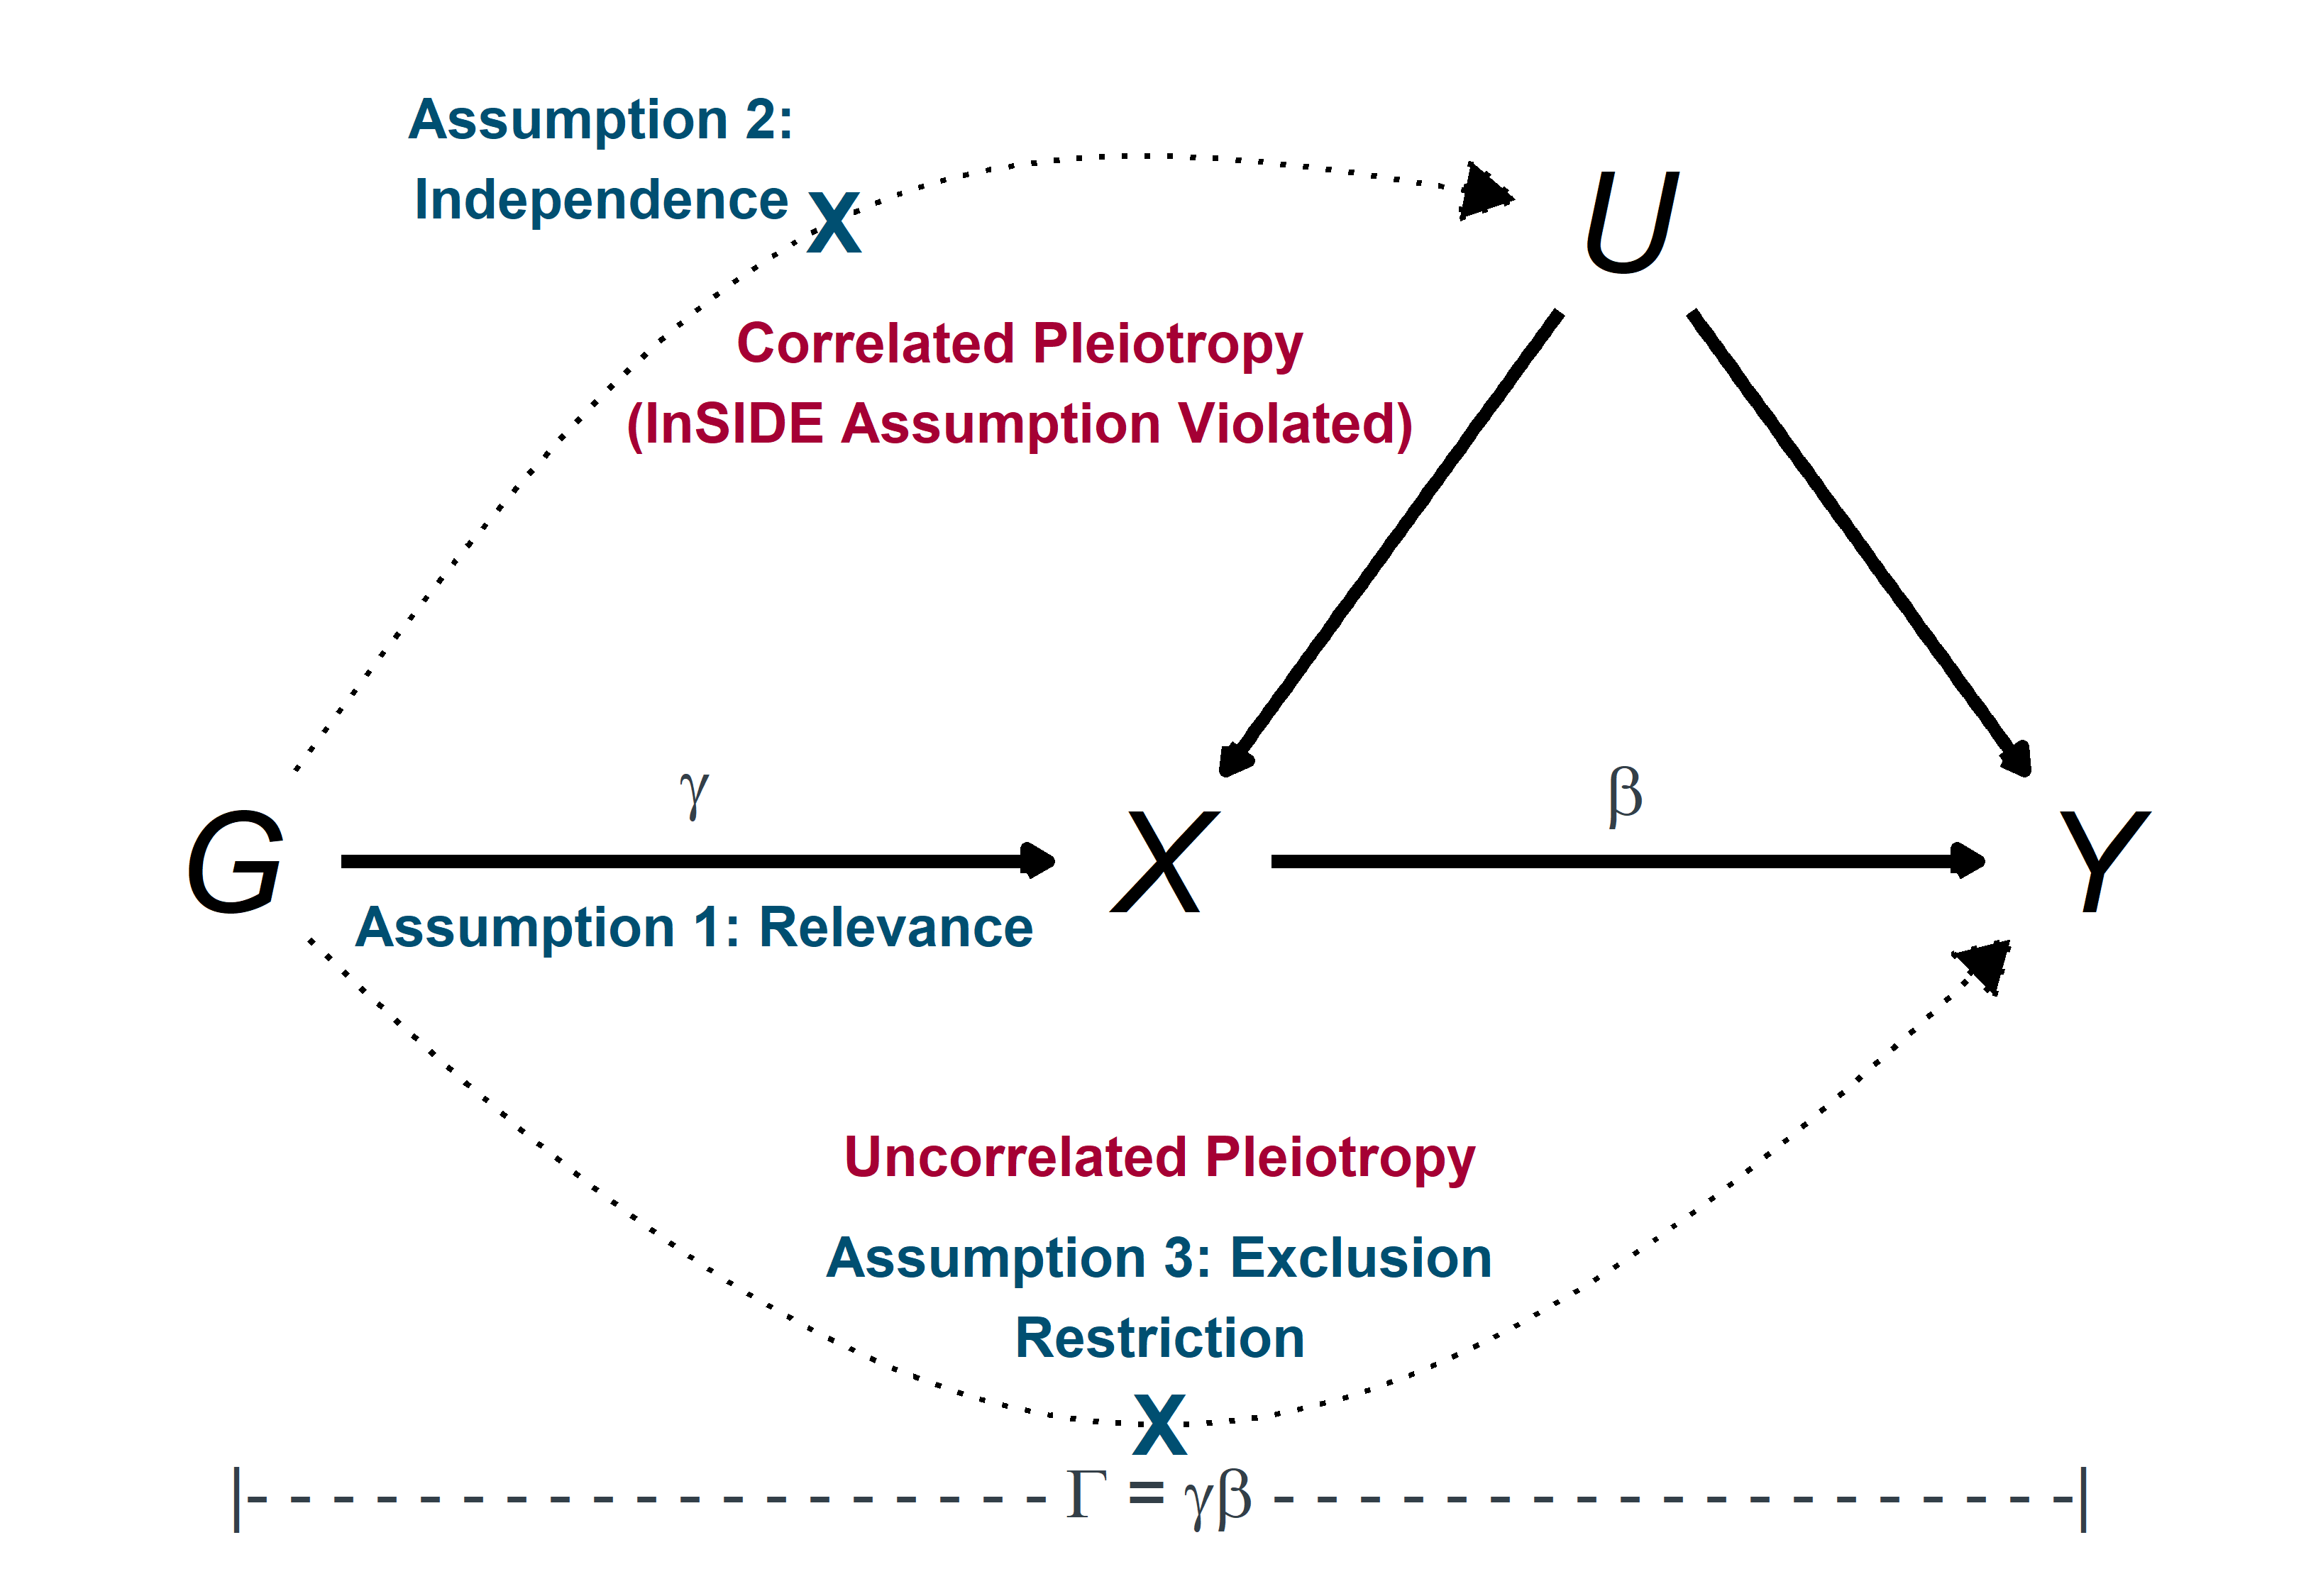
\includegraphics[keepaspectratio]{MSc_Thesis_Bookdown_files/figure-latex/DAG-assumptions-plot-1.png}}
\caption{\label{fig:DAG-assumptions-plot}Causal diagram illustrating the relationships between genetic instrument \emph{G}, exposure \emph{X}, outcome \emph{Y} and confounders of the exposure-outcome relationship \emph{U} in Mendelian randomisation studies. Blue text \& crosses represent key assumptions to ensure valid inference of causal effect of \emph{X} on \emph{Y} using \emph{G} as an instrumental variable. Red text represents violations of these assumptions that may lead to invalid inference through opening of alternate causal pathways. Greek characters represent the key parameters/association coefficients to be estimated. Adapted from Burgess et al 2016\textsuperscript{\citeproc{ref-burgess_sensitivity_2016}{7}}}
\end{figure}

Typically, \hyperref[acronyms_MR]{MR} studies estimate causal effect using a set of several genetic instruments; the causal effect estimate derived from the \(jth\) instrument is denoted \(\hat{\beta}_j\). Each estimate \(\hat{\beta}_j\) acknowledges there will be specific effects on the observed values of exposure and outcome given the presence of that specific genetic variant \(G_j\) under study, i.e.~\(\hat{\beta}_j\) is based on the instrument-conditioned exposure \({X|G_j}\) and the instrument-conditioned outcome \({Y|G_j}\). These observed values of exposure and outcome can be described by their own linear models:

\begin{equation} 
X|G_j = \gamma_0 + \gamma_j G_j + \epsilon_{X_j}
\end{equation}

\begin{equation} 
Y|G_j = \Gamma_0 + \Gamma_j G_j + \epsilon_{Y_j}
\end{equation}

where, for exposure and outcome respectively:

\begin{itemize}
\tightlist
\item
  \(\gamma_0\) and \(\Gamma_0\) reflect base values without any influence from the effect allele of the genetic variant
\item
  \(\gamma_j\) and \(\Gamma_j\) are coefficients of association with the genetic variant, representing the extent to which an effect allele of \(G_j\) will perturb the value of \(X\) or \(Y\) versus the non-effect allele
\item
  \(\epsilon_{X_j}\) and \(\epsilon_{Y_j}\) are error terms, containing contributions from confounders of the exposure-outcome relationship (\(U\) in the causal diagram), and all genetic variants except \(G_j\).
\end{itemize}

It can be shown that a simple causal effect estimate for the exposure on the outcome can be obtained from a single genetic instrument by the Wald method, dividing the coefficient of gene-outcome association by the coefficient of gene-exposure association, i.e.:

\begin{equation} 
\hat{\beta}_j = \frac {\hat{\Gamma}_j} {\hat{\gamma}_j}
\end{equation}

These coefficients of gene-exposure and gene-outcome association (\(\hat{\gamma}\) and \(\hat{\Gamma}\)) can be obtained from a \hyperref[acronyms_GWAS]{genome-wide association study (GWAS)}, which quantifies associations between small genetic variations - known as \hyperref[acronyms_SNP]{single nucleotide polymorphism (SNP)}s - and various phenotypes. Each genetic instrument selected from a \hyperref[acronyms_GWAS]{GWAS} may be valid or invalid, depending on it meeting the above assumptions. The overall causal effect estimate \(\hat{\beta}\) from any given \hyperref[acronyms_MR]{MR} method will typically seek to pool effect estimates from several instruments so as to minimise effects of any invalid instruments included, e.g.~by removing/down-weighting contributions of genetic instruments which violate one or more assumptions. This is equivalent to plotting all estimated coefficients of gene-outcome association (\(\bar{\Gamma}\)) versus all estimated coefficients of gene-exposure association (\(\bar{\gamma}\)) for the set of instruments, then using the gradient of a regression line through the points as the causal effect estimate \(\hat{\beta}\); picking an \hyperref[acronyms_MR]{MR} methodology is analogous to choosing the method to draw the line of best fit (Figure \ref{fig:Gamma-gamma-plot}). For binary outcomes, the causal effect estimate can be converted to an odds ratio (OR) through exponentiation, i.e.:

\begin{equation} 
OR = e^{\hat{\beta}}
\end{equation}

\begin{figure}
\centering
\pandocbounded{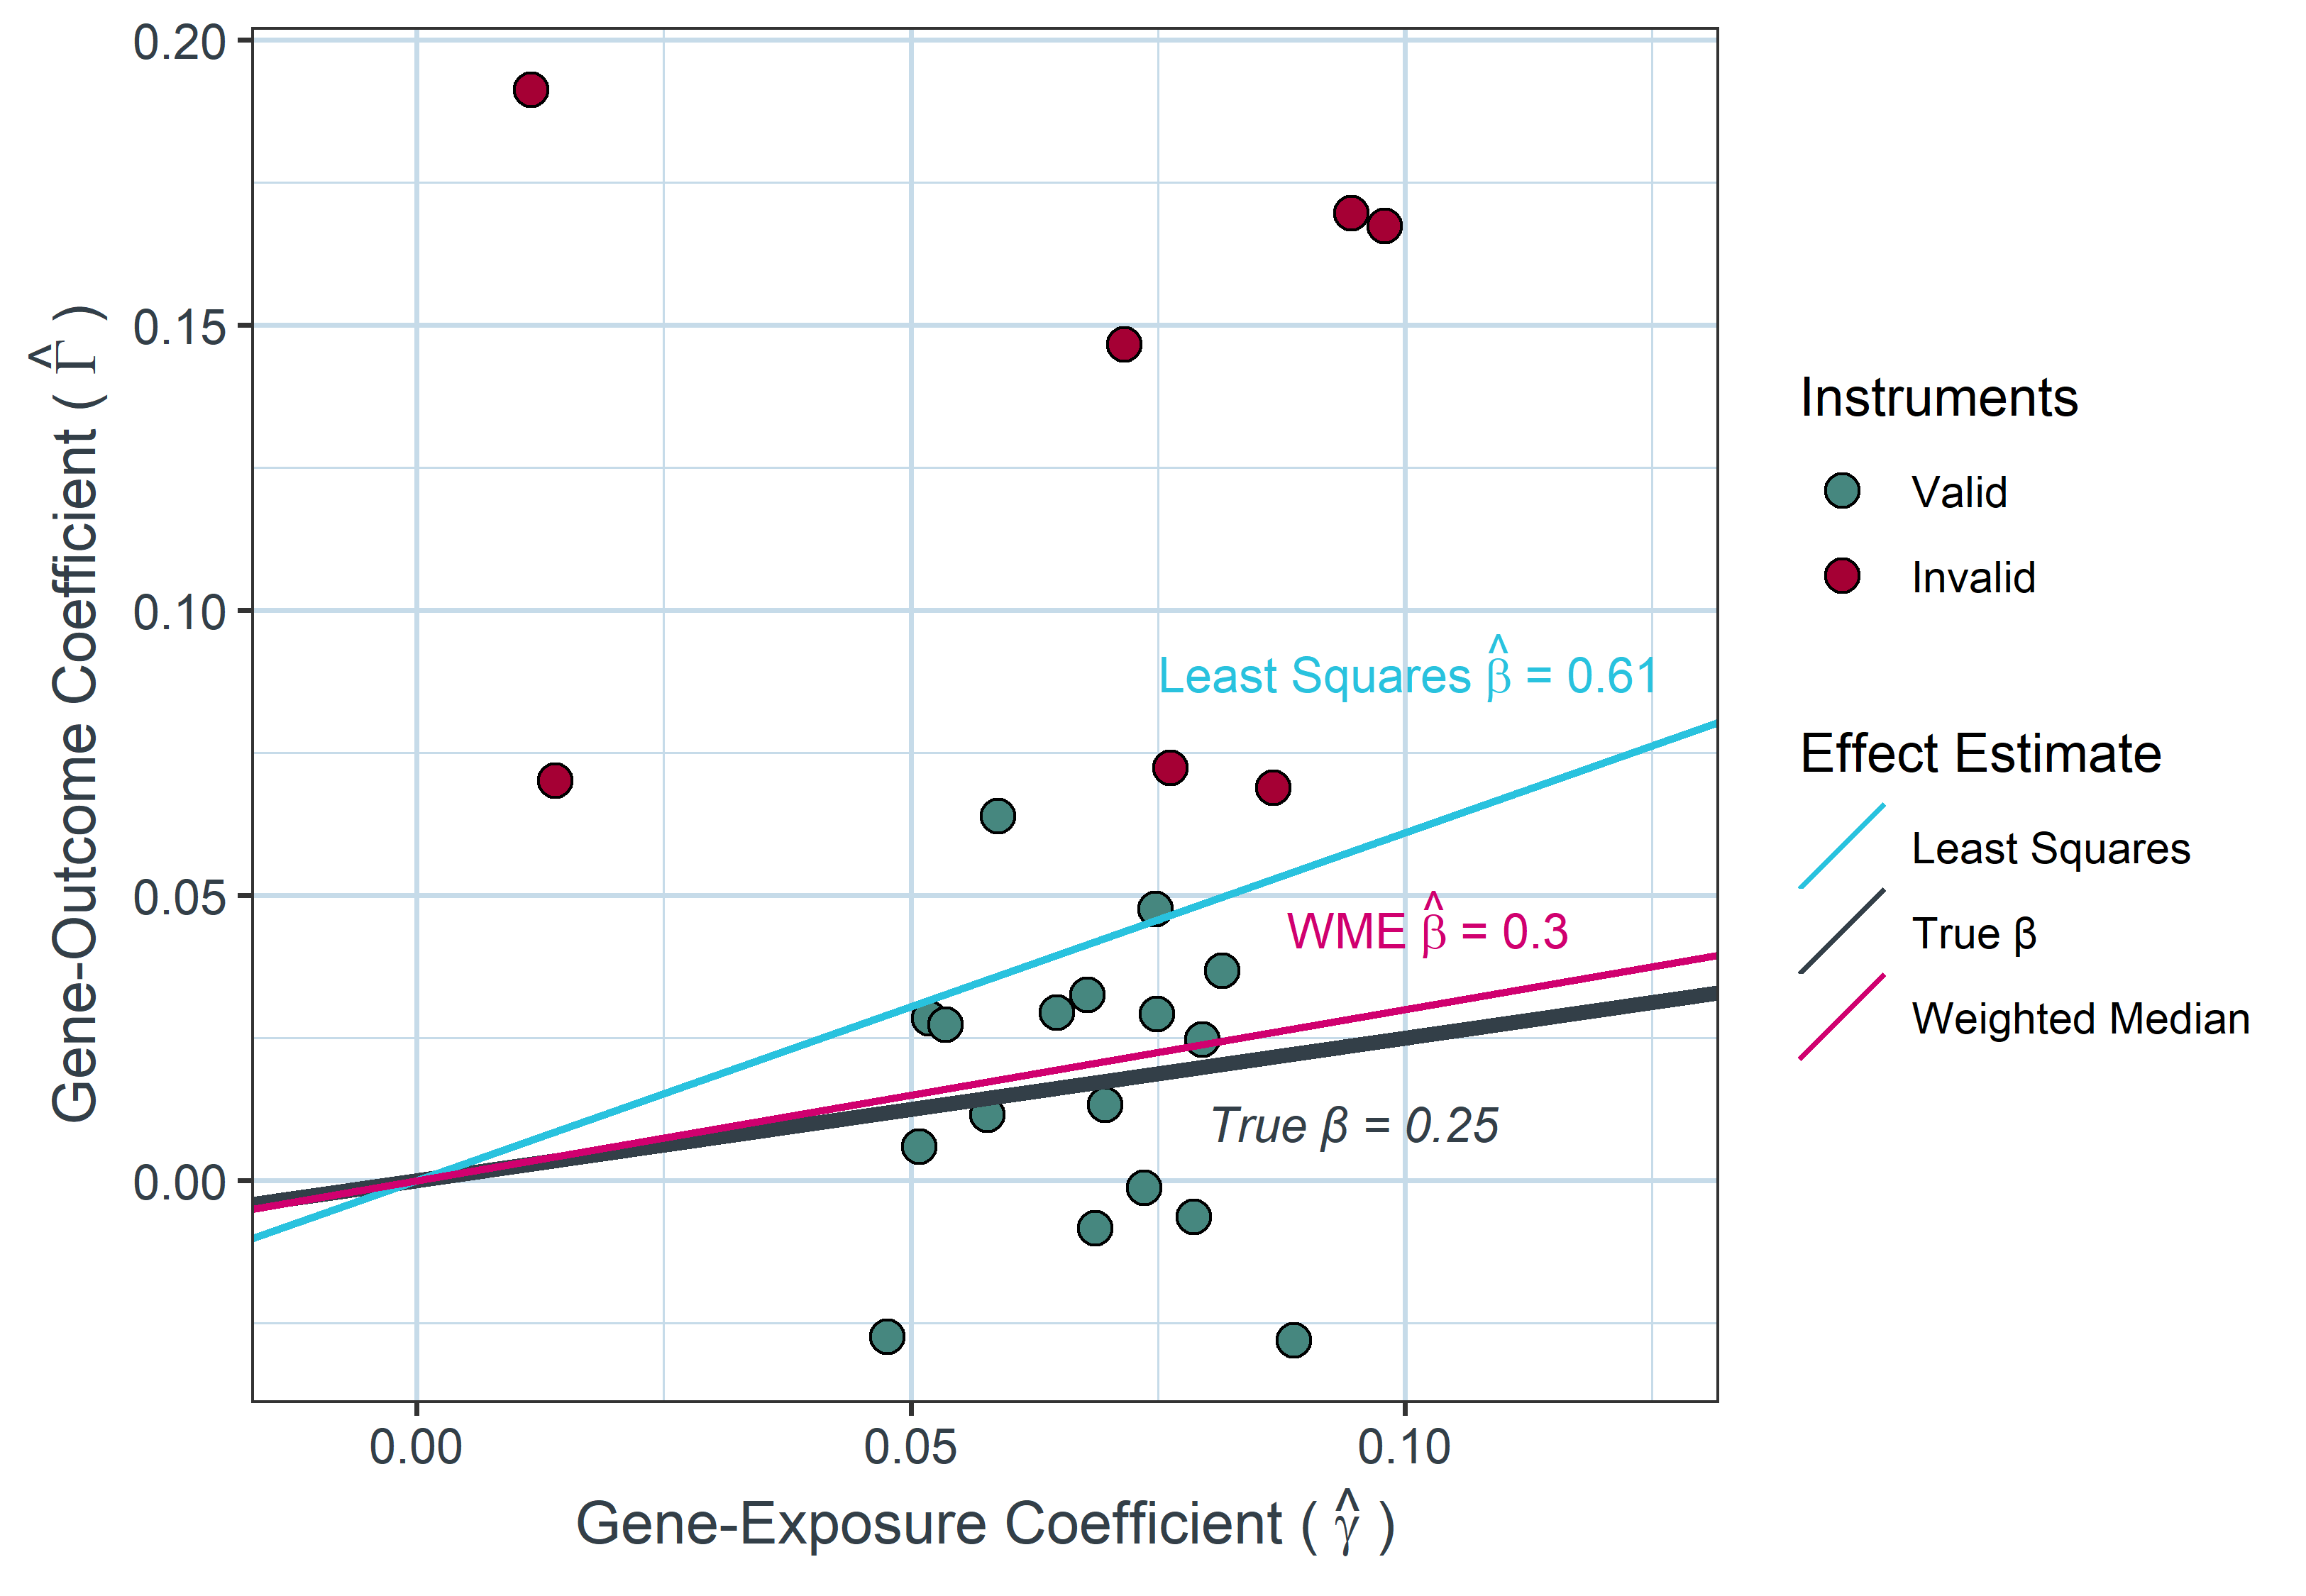
\includegraphics[keepaspectratio]{MSc_Thesis_Bookdown_files/figure-latex/Gamma-gamma-plot-1.png}}
\caption{\label{fig:Gamma-gamma-plot}Simulated MR Study on 10,000 individuals using 25 genetic instruments, of which 30\% are invalid (red points) and introduce directional pleiotropic effects. The true value of the exposure-outcome causal effect is 0.25 (grey line, causal effect represented by gradient). Regression using an unajusted least-squares linear model (light blue line) results in a biased estimate in the positive direction due to the influence of the invalid instruments. Using the Weighted Median Estimator method (pink line) attenuates the effects of the invalid instruments, resulting in an estimate closer to the true value. Adapted from Bowden et al 2016\textsuperscript{\citeproc{ref-bowden_consistent_2016}{8}}}
\end{figure}

\subsection{Violations to Assumptions}\label{violations-to-assumptions}

In practice, only the relevance assumption can be directly tested and proven. Typically, genetic variants for \hyperref[acronyms_MR]{MR} studies are selected as instruments based on their observed strength of association with exposures of interest in one or more \hyperref[acronyms_GWAS]{GWAS}. Sufficient gene-exposure association can be partly assured by selection using an appropriate genome-wide significance level (e.g.~\(p < 10 ^{-8}\)) during this instrument selection. Statistical testing can also further quantify the gene-exposure relationship; commonly used measures include the \(r^2\) statistic, representing the proportion of variance in the exposure explained by the genotype, and the related \(F\)-statistic, which additionally accounts for the the sample size under investigation\textsuperscript{\citeproc{ref-richmond_mendelian_2022}{9}}. An \(F\)-statistic of \(\ge\) 10 is generally considered to represent a strong enough gene-exposure association to consider a genetic instrument for use\textsuperscript{\citeproc{ref-martens_instrumental_2006}{2}}.

The assumptions of independence and exclusion restriction depend on all possible confounders of the exposure-outcome association, both measured and unmeasured; as such, these can never be proven absolutely. Various methods have been proposed to quantify and account for violations of these two additional assumptions, including the weighted median estimator, described below\textsuperscript{\citeproc{ref-bowden_consistent_2016}{8}}.

The main methods to avoid violations of the independence assumption relate to appropriate selection of populations studied to avoid confounding due to ancestry or population stratification. For example, in two-sample MR studies, where gene-exposure and gene-outcome coefficients are estimated from two separate \hyperref[acronyms_GWAS]{GWAS} studies, it is recommended to select \hyperref[acronyms_GWAS]{GWAS} studies performed in similar population groups (e.g.~both in Western Europeans). This practice helps avoid spurious exposure-outcome associations being generated by confounding due to underlying differences in e.g.~allele frequency, baseline disease risks etc between ancestrally different populations\textsuperscript{\citeproc{ref-richmond_mendelian_2022}{9}}.

Exclusion restriction is a particularly universal issue in MR, due to so-called (horizontal) genetic pleiotropy, where a single genetic variant may have multiple ``pleiotropic'' effects -- i.e.~it may influence several traits simultaneously. Such pleiotropic effects may be unknown and open unmeasured causal pathways between a genetic instrument and the outcome (Figure \ref{fig:DAG-assumptions-plot}), thus potentially biasing \hyperref[acronyms_MR]{MR} estimates of the association between exposure and outcome. As pleiotropy influences outcome separate to the path involving the exposure of interest, the term ``direct effects'' is also used\textsuperscript{\citeproc{ref-hemani_evaluating_2018}{10}}. Where pleiotropic effects are in both positive and negative directions with a mean of zero - ``balanced pleiotropy'' - then they only add noise to causal effect estimation\textsuperscript{\citeproc{ref-morrison_mendelian_2020}{11}}. By contrast, ``directional pleiotropy'', where the mean of pleiotropic effects is non-zero, may introduce bias\textsuperscript{\citeproc{ref-bowden_consistent_2016}{8}} (Figure \ref{fig:Gamma-gamma-plot}).

If such an additional causal pathway acts between gene \(G\) and outcome \(Y\) via a confounding factor \(U\), then the magnitude of direct/overall effects of \(G\) on \(Y\) will correlate with the effects of \(G\) on \(X\) (i.e.~\(\Gamma \propto \gamma\)), and ``correlated pleiotropy'' is present. If an additional causal pathway acts directly between gene \(G\) and outcome \(Y\) independent of both exposure \(X\) and confounders \(U\), this results in ``uncorrelated pleiotropy'' (Figure \ref{fig:DAG-assumptions-plot}). Both correlated and uncorrelated pleiotropy can introduce bias which distorts the estimate of the true causal effect. In general, correlated pleiotropy is more challenging to account for; several MR methods explicitly require an additional assumption of \hyperref[acronyms_InSIDE]{Instrument Strength Independent of Direct Effect (InSIDE)}, i.e no correlated pleiotropy to be present\textsuperscript{\citeproc{ref-grant_bayesian_2024}{12}}.

\subsection{Weighted Median Estimator (WME)}\label{weighted-median-estimator-wme}

A common approach to produce exposure-outcome causal effect estimates robust to violations of the exclusion restriction assumption is the \hyperref[acronyms_WME]{weighted median estimator (WME)} method, proposed by Bowden et al\textsuperscript{\citeproc{ref-bowden_consistent_2016}{8}}.

In \hyperref[acronyms_WME]{WME} analysis, several genetic instruments are used to estimate the exposure-outcome causal effect \(\hat{\beta}\). Each instrument is known to be associated with the exposure of interest, but an unknown proportion of these instruments may be invalid due to pleiotropic genetic effects. Any instrument linked to an outcome via multiple pleiotropic causal pathways will exhibit a less consistent gene-outcome association than a relationship mediated by a single pathway; this results in larger variance in causal estimates derived from invalid/pleiotropic genetic instruments versus estimates from valid instruments.

\hyperref[acronyms_WME]{WME} therefore assigns a weight to each genetic instrument's estimate of the causal effect according to the inverse of the variance of the estimate; these weighted effect estimates are used to construct a cumulative distribution function for probability of true causal effect size across the range of estimated values. The 50th percentile of this distribution can then be taken as a ``weighted median estimate'' of the true causal effect, theoretically producing consistent causal estimates even if up to 50\% of the included information comes from invalid instruments\textsuperscript{\citeproc{ref-bowden_consistent_2016}{8}}. An example of \hyperref[acronyms_WME]{WME} attenuating the effects of invalid instruments is shown in Figure \ref{fig:Gamma-gamma-plot}.

\subsection{Issues With WME CIs}\label{issues-with-wme-cis}

\hyperref[acronyms_WME]{WME} calculation methods are available via several prolific \hyperref[acronyms_MR]{MR} tools: the R packages ``MendelianRandomization''\textsuperscript{\citeproc{ref-yavorska_mendelianrandomization_2017}{13}} and ``TwoSampleMR'', and the MR-Base web platform\textsuperscript{\citeproc{ref-hemani_mr-base_2018}{14}}. However, these implement the original authors' suggested process of generating 95\% confidence intervals for \hyperref[acronyms_WME]{WME}, which deviates from accepted re-sampling methodology:

\begin{quote}
``We found the bootstrap confidence interval\ldots too conservative. However, the bootstrap standard error\ldots{} gave more reasonable coverage using a normal approximation (estimate ±1.96 x standard error) to form a 95\% confidence interval''\textsuperscript{\citeproc{ref-bowden_consistent_2016}{8}}
\end{quote}

This modification, explicitly aiming to boost estimate precision artificially, would be expected to lead to a high Type 1 error rate, which has been a growing concern in the field of late\textsuperscript{\citeproc{ref-stender_reclaiming_2024}{15}}. The theoretical issues with this approach, and the fundamentals of bootstrapping in general, are covered in Appendix \ref{appendix-boot}.

\subsection{MR-Hevo}\label{mr-hevo}

MR-Hevo is an R package which uses more typical Bayesian methodology to estimate MR causal effects and corresponding 95\% confidence intervals. It uses the probabilistic programming language, Stan, to directly sample the posterior probability distribution of pleiotropic effects on the outcome, rather than making untested assumptions about the shape of this distribution as current \hyperref[acronyms_WME]{WME} implementations do\textsuperscript{\citeproc{ref-mckeigue_inference_2024}{16}} (Appendix \ref{appendix-boot}).

MR-Hevo incorporates several additional features which its creators claim further aid valid causal inference. Most MR analyses only account for one genetic variant per genetic locus (i.e.~per location in the genome). If multiple variants exist at a given locus, generally only one will be selected as an instrument for further \hyperref[acronyms_MR]{MR} analysis. MR-Hevo can handle multiple instruments per genetic locus via scalar construction, essentially assigning a ``score'' to each locus based on the variant(s) present, thus incorporating more information than if closely grouped variants had been discarded\textsuperscript{\citeproc{ref-mckeigue_inference_2024}{16}}. As MR-Hevo is based on a Bayesian approach, it generates estimates which incorporate relevant existing information generated by prior studies, increasing the amount of data informing each estimate. In this case, MR-Hevo bases estimates on a prior probability distribution which reflects existing knowledge that most individual genetic instruments will have only small effects on complex traits\textsuperscript{\citeproc{ref-park_estimation_2010}{17},\citeproc{ref-piironen_sparsity_2017}{18}}, further aiding biologically plausible inference regarding distribution of pleiotropic effects.

\subsection{Aims and Objectives}\label{aims-and-objectives}

The main aim of this study will be compare the performance and conclusions of MR-Hevo versus \hyperref[acronyms_WME]{WME} causal effect estimation methods in \hyperref[acronyms_MR]{MR} studies. In particular, this study aims to demonstrate if the \hyperref[acronyms_WME]{WME} approach gives over-confident causal estimates in the presence of pleiotropy, and whether this issue is more correctly handled by the MR-Hevo approach as its creators suggest. This will be achieved through addressing the research questions and objectives as outlined below:

\subsubsection*{Research Questions:}\label{research-questions}
\addcontentsline{toc}{subsubsection}{Research Questions:}

\begin{enumerate}
\def\labelenumi{\arabic{enumi}.}
\tightlist
\item
  How does MR-Hevo perform versus the weighted median estimator when estimating causal effects in MR studies?
\item
  Do conclusions of existing MR studies using weighted median causal effect estimation change if MR-Hevo methods are used?
\end{enumerate}

\subsubsection*{Objectives:}\label{objectives}
\addcontentsline{toc}{subsubsection}{Objectives:}

\begin{enumerate}
\def\labelenumi{\arabic{enumi}.}
\tightlist
\item
  Quantify the accuracy and precision of MR-Hevo causal estimates for simulated data under differing sets of common assumptions, with reference to the weighted median estimator
\item
  Evaluate the consistency of MR-Hevo causal estimates for simulated data under differing sets of common assumptions, with reference to the weighted median estimator
\item
  Compare the conclusions drawn from MR-Hevo causal effect estimation versus the weighted median estimator on real-world data
\end{enumerate}

\newpage

\section{Methods}\label{Methods}

\subsection{Simulation Study}\label{simulation-study}

To establish the performance of MR-Hevo causal estimation relative to WME, the accuracy, precision and consistency of both methods were evaluated using simulated datasets with known parameter values.

\subsubsection{Data Simulation}\label{data-simulation}

To aid comparability with existing methods and literature, the simulation methodology of the original WME exposition was reproduced based on published models and parameters in Appendix 3 of its supplementary materials\textsuperscript{\citeproc{ref-bowden_consistent_2016}{8}}. Full details of simulation reproduction, including code and validation of outputs, is presented in Appendix \ref{appendix-sim}.

In brief, simulations were created based on three different scenarios, each representing a common set of assumptions about underlying data used for MR, and each increasingly challenging to the performance of any given MR causal estimation methodology:

\begin{enumerate}
\def\labelenumi{\arabic{enumi}.}
\item
  Balanced pleiotropy, InSIDE assumption satisfied - A proportion of invalid genetic instruments are present and introduce pleiotropic effects uncorrelated with the instrument strength; these pleiotropic effects are equally likely to be positive as negative with a mean value = 0, thus introducing noise into the estimation of causal effect.
\item
  Directional pleiotropy, InSIDE assumption satisfied - A proportion of invalid genetic instruments are present and introduce pleiotropic effects uncorrelated with the instrument strength; these pleiotropic effects are positive only, with a mean value \textgreater{} 0, thus biasing the causal effect estimate in a positive direction.
\item
  Directional pleiotropy, InSIDE assumption not satisfied - A proportion of invalid genetic instruments are present and introduce pleiotropic effects correlated with the instrument strength through action via a confounder; these pleiotropic effects are positive only, with a mean value \textgreater{} 0, thus potentially biasing the causal effect estimate in a positive direction to an even greater extent than Scenario 2.
\end{enumerate}

1,000 simulated datasets of participant-level data were generated for every combination of each scenario and each the following simulation parameters:

\begin{itemize}
\tightlist
\item
  Proportion of invalid instruments: 0\%, 10\%, 20\% or 30\%
\item
  Number of participants: \(n = 10,000\) or \(n = 20,000\)
\item
  Causal effect: null (\(\beta = 0\)) or positive (\(\beta = 0.1\))
\end{itemize}

The same set of 25 simulated genetic instruments were used across all datasets, with the status of each as valid/invalid determined by random draw per instrument at the start of each simulation run of 1,000 datasets.

Genotypes were simulated as for a two-sample setting: where number of particpants was \(n = 10,000\), then 20,000 genotypes were simulated - 10,000 for the cohort used to estimate gene-exposure association (\(\hat{\gamma}\)), and a separate cohort of 10,000 used to estimate gene-outcome association (\(\hat{\Gamma}\)). Parameter values for effect allele frequency were not specified by Bowden et al, though initial testing showed values around 0.5 produced WME causal effect estimates closest to published values when other parameters were matched\textsuperscript{\citeproc{ref-bowden_consistent_2016}{8}}. As such, effect allele frequencies were assigned per instrument from a uniform distribution between 0.4 to 0.6. Each effect allele freqency thus generated per instrument was then used as a probability to assign each simulated participant effect alleles for each instrument via two draws from a binomial distribution.

\subsubsection{Analysis of Simulated Data}\label{analysis-of-simulated-data}

Each dataset generated was analysed using both WME and MR-Hevo methods, via functions from the \texttt{TwoSampleMR} and \texttt{mrhevo} packages, respectively\textsuperscript{\citeproc{ref-hemani_mr-base_2018}{14},\citeproc{ref-mckeigue_inference_2024}{16}}. Results were aggregated per group of 1,000 simulated datasets corresponding to a particular combination of scenario and parameter values. This resulted in one meta-analysis reported per combination of scenario/parameter values, each including 1,000 simulated MR studies using the same 25 genetic instruments in the same population. Aggregated measures for both WME and MR-Hevo per meta-analysis were mean causal effect estimate; mean standard errors/\hyperref[acronyms_CI]{confidence interval (CI)}s of the causal effect estimate; and causality report rate, i.e.~percentage of simulated studies reported as a non-null causal effect with a 95\% \hyperref[acronyms_CI]{CI} for the causal effect estimate not including 0.

Results of the above aggregations were tabulated as per Tables 2 \href{https://pmc.ncbi.nlm.nih.gov/articles/PMC4849733/table/gepi21965-tbl-0002/}{(link)} and 3\href{https://pmc.ncbi.nlm.nih.gov/articles/PMC4849733/table/gepi21965-tbl-0003/}{(link)} of Bowden et al\textsuperscript{\citeproc{ref-bowden_consistent_2016}{8}} to allow direct comparisons of both methods versus each other and versus the published characteristics of existing MR causal estimation methods.

\subsection{Re-Analysis of Published Data}\label{re-analysis-of-published-data}

To investigate the potential implications of any differences in performance between WME and MR-Hevo methods, a selection of published studies reporting causal effect estimates using the WME method was re-analysed. A sample size of 10 published studies was decided as a pragmatic compromise between the scope of this project and the need to check consistency of any observed differences. In the original Bowden et al simulation studies, the WME causal estimation method was shown to generate a false-positive report rate of \(\ge\) 30\% with relatively minor violations of relevant assumptions\textsuperscript{\citeproc{ref-bowden_consistent_2016}{8}}; therefore, even this relatively small sample of 10 studies might be expected to demonstrate differences between methods if the MR-Hevo approach is as appropriately conservative as its creators propose.

To estimate the upper bound of the potential impact of MR-Hevo versus existing WME methodology, studies were chosen for re-analysis based on their number of citations in the wider MR literature. Compared to studies with few or no citations, highly-cited studies would be expected to have a larger impact on their respective fields if their conclusions were to change. In addition, highly-cited works will typically have been submitted to more scrutiny than less-cited works - both during peer review whilst under consideration by journals likely to produce highly-cited works, and from the wider scientific community following the widespread dissemination evidenced by a high citation count. As such, it would be expected that highly-cited works are likely to be free of significant methodological flaws which may impede interpretation of any re-analysis.

\subsubsection{Citation Search}\label{citation-search}

The Scopus search platform\textsuperscript{\citeproc{ref-noauthor_scopus_nodate}{19}} was used on 15/04/2025 to retrieve all articles citing the original weighted median estimator exposition paper\textsuperscript{\citeproc{ref-bowden_consistent_2016}{8}}. The articles returned were sorted by the number of times each article itself had been cited, and the resulting list was saved to RIS format in blocks of ten articles for upload into the Covidence evidence synthesis platform\textsuperscript{\citeproc{ref-noauthor_covidence_2025}{20}}. Abstracts were screened by a single reviewer (B233241), starting with the most cited article and proceeding in descending order of citation count, against the following inclusion and exclusion criteria:

Inclusion criteria:

\begin{itemize}
\item
  Original two-sample MR study
\item
  Able to determine samples' ancestry sufficient to establish presence/potential degree of participant overlap between groups
\item
  Reporting \(\ge\) 20 human genetic instruments relating to exposure
\item
  Reports details of effect/non-effect alleles
\item
  Regression coefficients and standard errors and/or confidence intervals available for each genetic instrument used
\item
  Uses Weighted Median Estimator
\end{itemize}

Exclusion criteria:

\begin{itemize}
\item
  Methodology paper, review article, editorial or letter
\item
  English full-text not accessible
\end{itemize}

Where eligibility could not be determined from abstract screening alone, full texts were retrieved and screened against the same criteria. Screening of abstracts and full texts was undertaken in blocks of ten articles, until the target of ten included studies for reanalysis had been reached.

Where an article reported multiple exposure-outcome associations, data were only extracted for the association with the highest number of genetic instruments available, or else for the first reported association where several were based on the same number of instruments. Data were extracted from full texts of included studies using a standardised data collection template, which included publication details, citation count, primary study question, degree of potential participant overlap between groups, number/details of genetic instruments used, effect estimates/standard errors calculated, and conclusion regarding causality as determined by the weighted median estimator method.

\subsection{Data Manipulation and Analysis}\label{data-manipulation-and-analysis}

All simulations, data manipulations and data analyses were performed in R version 4.4.1 (2024-06-14 ucrt)\textsuperscript{\citeproc{ref-base}{21}}.

For the simulation study, full details of computation are available in Appendix \ref{appendix-sim}.

For citation search data, a standardised data collection form was Microsoft Excel\textsuperscript{\citeproc{ref-microsoft_corporation_microsoft_2018}{22}} to create .csv files for subsequent analysis in R; Excel's ``Get Data'' function was also used to extract tables of genetic instruments where these were presented in non-csv format (e.g.~pdf).

Data cleaning for citation search data was primarily undertaken using the Tidyverse suite of R packages\textsuperscript{\citeproc{ref-tidyverse}{23}}. A full list of packages used can be found in Appendix \ref{appendix-pkg}.

Data were manually screened at summary level and relevant features were extracted. Data were checked for completeness, consistency, duplicate values and plausibility. Data were transformed to an appropriate data type, and encoding of genetic variables was standardised into a single format. Missing values for association coefficients and \hyperref[acronyms_SE]{standard error (SE)}s were imputed as the mean value calculated per dataset. It was noted during early testing that causal effect estimation functions did not operate correctly in the presence of zero-value coefficients of genetic association and/or their standard errors; such zero values were therefore re-coded as an arbitrarily low value of \(10^{-100}\).

\subsection{Ethical Approval}\label{ethical-approval}

The protocol for this work has been reviewed and approved by the \hyperref[acronyms_UMREG]{Usher Masters Research Ethics Group (UMREG)} at the University of Edinburgh, Ethics ID: UM241126. Due to the nature of the project, using simulated and publically available data only, no significant ethical issues were foreseen, and sponsorship was deemed unnecessary by the \hyperref[acronyms_UMREG]{UMREG} reviewing panel.

\section{Results}\label{results-1}

\subsection{Simulation Study}\label{simulation-study-1}

\subsubsection{Data Simulation}\label{data-simulation-1}

Data were successfully simulated as intended. A selection of representative visualisations are presented in Figure \ref{fig:data-sim-validation}. Full details of testing used to validate model outputs from parameter inputs are given in Appendix \ref{appendix-sim-test}. The \(F\)-statistic calculated from simulated instruments was \textgreater10, indicating that they were sufficiently strongly associated with exposure to meet the relevance assumption of \hyperref[acronyms_IV]{IV} analysis (Tables \ref{tab:no-causal-sim-summ-display} and \ref{tab:causal-sim-summ-display}).

\begin{figure}
\centering
\pandocbounded{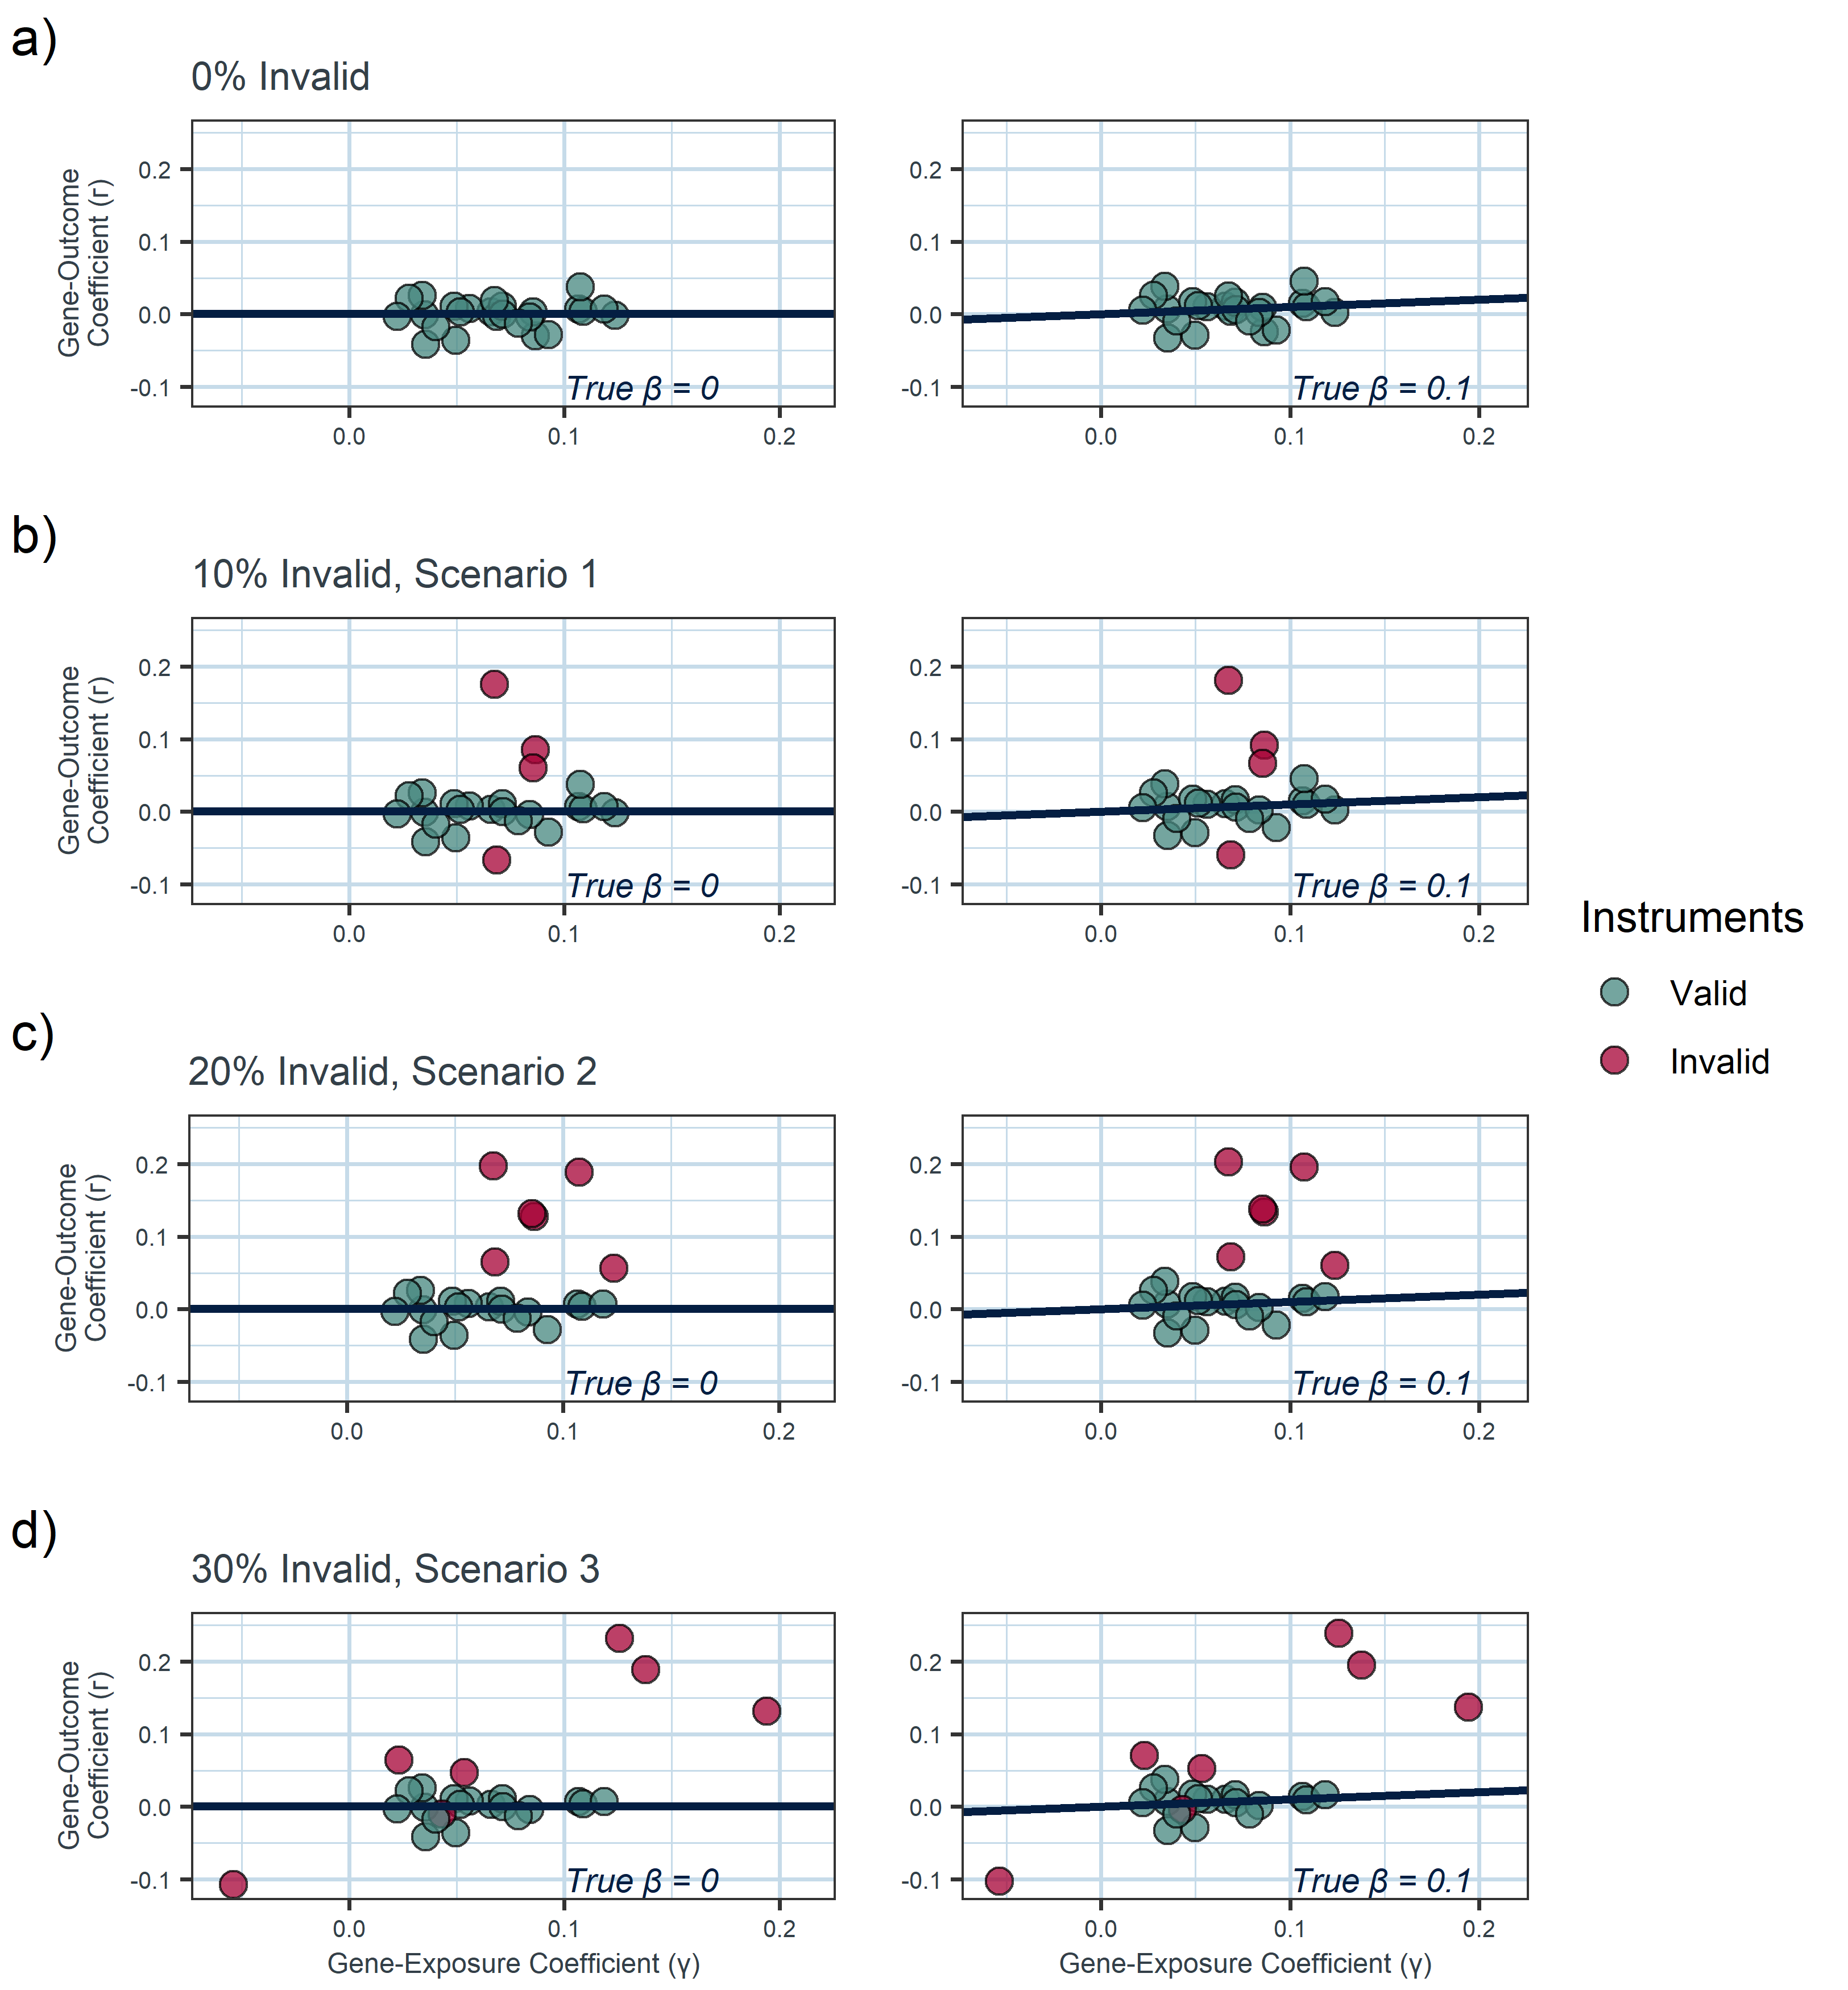
\includegraphics[keepaspectratio]{MSc_Thesis_Bookdown_files/figure-latex/data-sim-validation-1.png}}
\caption{\label{fig:data-sim-validation}Plots of a representative group of simulated datasets; all simulate genetic instruments from the same index from the same random seed. Left and right columns demonstrate null and positive true causal effects, respectively; the true causal effect is represented by the gradient of the line shown. The scenario and the proportion of invalid (i.e.~pleiotropic) genetic instruments changes with each row. a) 0\% of instruments invalid, rendering scenario assumptions regarding invalid assumptions irrelevant. b) 10\% of instruments invalid, Scenario 1: balanced pleiotropy introduces noise around the causal effect. c) 20\% of instruments invalid, Scenario 2: directional pleiotropy biases in the direction of the invalid instruments. d) 30\% of instruments invalid, Scenario 3: directional pleiotropy and InSIDE assumption violation strongly biases towards a positive effect estimate.}
\end{figure}

\subsubsection{Analysis of Simulated Data}\label{analysis-of-simulated-data-1}

\paragraph{No Causal Effect}\label{results-sim-no-causal}

\leavevmode\newline Across all cases where no causal effect was present (Table \ref{tab:no-causal-sim-summ-display}), the mean rate of reporting a causal effect (i.e.~false-positive rate) for MR-Hevo was 0.41\% versus 5.1\% for \hyperref[acronyms_WME]{WME}. Of the 24 combinations of scenarios and parameters, MR-Hevo exhibited a favourable false-positive rate versus \hyperref[acronyms_WME]{WME} in 24 (100\%).

For both MR-Hevo and \hyperref[acronyms_WME]{WME} methods, false-positive report rates generally increased with an increasing proportion of invalid instruments up to around 20\% invalid \hyperref[acronyms_IV]{IV}s. As assumption violations progressively presented greater data variability and bias across scenarios 1 to 3, both MR-Hevo and \hyperref[acronyms_WME]{WME} methods tended to exhibit higher false-positive report rates, though this progression was noticably attenuated for MR-Hevo versus \hyperref[acronyms_WME]{WME}, particularly under the assumptions of Scenario 3. Both trends across invalid instrument proportions and scenarios were somewhat attenuated by increasing sample size from 10,000 to 20,000 participants for both methods.

The mean causal effect estimate (mean reported 95\% \hyperref[acronyms_CI]{CI}s) across all cases was 0.04 (-0.11 to 0.2) for MR-Hevo and 0.039 (-0.11 to 0.19) for \hyperref[acronyms_WME]{WME}. For \hyperref[acronyms_SE]{SE}, the mean (range) \hyperref[acronyms_SE]{SE} of causal effect estimates across all cases was 0.0012 (0 to 0.002) for MR-Hevo and 0.076 (0.056 to 0.099) for \hyperref[acronyms_WME]{WME}.

Causal effect estimates, width of \hyperref[acronyms_CI]{CI}s and \hyperref[acronyms_SE]{SE} all tended to increase slightly for each method, both with an increasing proportion of invalid instruments up to 20\% invalid \hyperref[acronyms_IV]{IV}s, and as assumption violations progressively presented greater data variability and bias across scenarios 1 to 3. For both these trends, MR-Hevo estimates tended to be more affected than those from \hyperref[acronyms_WME]{WME}, in contrast to the false-positive report rates, though MR-Hevo causal effect estimates were once more relatively less affected by Scenario 3 assumptions. Again, both trends across differing scenarios and invalid instrument proportions were somewhat attenuated by increasing sample size from 10,000 to 20,000 participants for both methods.

\paragraph{Positive Causal Effect}\label{results-sim-causal}

\leavevmode\newline Across all cases where no causal effect was present (Table \ref{tab:causal-sim-summ-display}), the mean rate of reporting a causal effect (i.e.~sensitivity) for MR-Hevo was 31\% versus 28\% for \hyperref[acronyms_WME]{WME}. Of the 24 combinations of scenarios and parameters, MR-Hevo exhibited a favourable sensitivity versus \hyperref[acronyms_WME]{WME} in 10 (42\%).

For both MR-Hevo and \hyperref[acronyms_WME]{WME} methods, causal report rates increased with an increasing proportion of invalid instruments up to around 20\% invalid \hyperref[acronyms_IV]{IV}s, though this was more consistent for \hyperref[acronyms_WME]{WME} versus MR-Hevo. As assumption violations progressively presented greater data variability and bias across scenarios 1 to 3, both MR-Hevo and \hyperref[acronyms_WME]{WME} methods tended to exhibit higher causal report rates. Both trends across differing scenarios and invalid instrument proportions were somewhat attenuated by increasing sample size from 10,000 to 20,000 participants for both methods, which also generally increased sensitivity for each method.

The mean causal effect estimate (mean reported 95\% \hyperref[acronyms_CI]{CI}s) across all cases was 0.13 (-0.025 to 0.3) for MR-Hevo and 0.11 (-0.039 to 0.26) for \hyperref[acronyms_WME]{WME}. For \hyperref[acronyms_SE]{SE}, the mean (range) \hyperref[acronyms_SE]{SE} of causal effect estimates across all cases was 0.0013 (0.001 to 0.002) for MR-Hevo and 0.077 (0.056 to 0.1) for \hyperref[acronyms_WME]{WME}.

Causal effect estimates, width of \hyperref[acronyms_CI]{CI}s and \hyperref[acronyms_SE]{SE} all tended to increase slightly for each method with an increasing proportion of invalid instruments up to 20-30\% invalid \hyperref[acronyms_IV]{IV}s; MR-Hevo estimates tended to be more affected by proportion of invalid instruments compared to \hyperref[acronyms_WME]{WME} estimates. As assumption violations progressively presented greater data variability and bias across scenarios 1 to 3, \hyperref[acronyms_WME]{WME} causal estimates tended to increase across all three; MR-Hevo estimates increased when switching from Scenario 1 to Scenario 2, but were relatively unaffected in Scenario 3 versus Scenario 2. Again, trends across invalid instrument proportions were somewhat attenuated by increasing sample from 10,000 to 20,000 participants for both methods, though the effects of sample size on trends across scenarios was less obvious.

\newpage

\global\setlength{\Oldarrayrulewidth}{\arrayrulewidth}

\global\setlength{\Oldtabcolsep}{\tabcolsep}

\setlength{\tabcolsep}{2pt}

\renewcommand*{\arraystretch}{1.3}



\providecommand{\ascline}[3]{\noalign{\global\arrayrulewidth #1}\arrayrulecolor[HTML]{#2}\cline{#3}}

\begin{longtable}[c]{|p{0.44in}|p{0.57in}|p{0.35in}|p{0.38in}|p{0.51in}|p{0.45in}|p{0.65in}|p{0.44in}|p{0.19in}|p{0.51in}|p{0.45in}|p{0.65in}|p{0.44in}}

\caption{Summary\ of\ 1,000\ simulated\ Mendelian\ randomisation\ studies\ per\ combination\ of\ scenario\ and\ parameters,\ all\ with\ null\ causal\ effect}\label{tab:no-causal-sim-summ-display}\\

\ascline{1.5pt}{666666}{1-13}

\multicolumn{1}{>{\centering}m{\dimexpr 0.44in+0\tabcolsep}}{} & \multicolumn{1}{>{\centering}m{\dimexpr 0.57in+0\tabcolsep}}{} & \multicolumn{1}{>{\centering}m{\dimexpr 0.35in+0\tabcolsep}}{} & \multicolumn{1}{>{\centering}m{\dimexpr 0.38in+0\tabcolsep}}{} & \multicolumn{4}{>{\centering}m{\dimexpr 2.06in+6\tabcolsep}}{\textcolor[HTML]{000000}{\fontsize{9}{9}\selectfont{\global\setmainfont{Arial}{Weighted}}}} & \multicolumn{1}{>{\centering}m{\dimexpr 0.19in+0\tabcolsep}}{\textcolor[HTML]{000000}{\fontsize{9}{9}\selectfont{\global\setmainfont{Arial}{}}}} & \multicolumn{4}{>{\centering}m{\dimexpr 2.06in+6\tabcolsep}}{\textcolor[HTML]{000000}{\fontsize{9}{9}\selectfont{\global\setmainfont{Arial}{MR}}}} \\





\multicolumn{1}{>{\centering}m{\dimexpr 0.44in+0\tabcolsep}}{} & \multicolumn{1}{>{\centering}m{\dimexpr 0.57in+0\tabcolsep}}{} & \multicolumn{1}{>{\centering}m{\dimexpr 0.35in+0\tabcolsep}}{} & \multicolumn{1}{>{\centering}m{\dimexpr 0.38in+0\tabcolsep}}{} & \multicolumn{4}{>{\centering}m{\dimexpr 2.06in+6\tabcolsep}}{\textcolor[HTML]{000000}{\fontsize{9}{9}\selectfont{\global\setmainfont{Arial}{Median}}}} & \multicolumn{1}{>{\centering}m{\dimexpr 0.19in+0\tabcolsep}}{\textcolor[HTML]{000000}{\fontsize{9}{9}\selectfont{\global\setmainfont{Arial}{}}}} & \multicolumn{4}{>{\centering}m{\dimexpr 2.06in+6\tabcolsep}}{\textcolor[HTML]{000000}{\fontsize{9}{9}\selectfont{\global\setmainfont{Arial}{Hevo}}}} \\

\ascline{1pt}{000000}{5-8}\ascline{1pt}{000000}{10-13}



\multicolumn{1}{>{\centering}m{\dimexpr 0.44in+0\tabcolsep}}{} & \multicolumn{1}{>{\centering}m{\dimexpr 0.57in+0\tabcolsep}}{} & \multicolumn{1}{>{\centering}m{\dimexpr 0.35in+0\tabcolsep}}{} & \multicolumn{1}{>{\centering}m{\dimexpr 0.38in+0\tabcolsep}}{} & \multicolumn{2}{>{\centering}m{\dimexpr 0.96in+2\tabcolsep}}{\textcolor[HTML]{000000}{\fontsize{9}{9}\selectfont{\global\setmainfont{Arial}{Mean\ Estimate}}}} & \multicolumn{1}{>{\centering}m{\dimexpr 0.65in+0\tabcolsep}}{\textcolor[HTML]{000000}{\fontsize{9}{9}\selectfont{\global\setmainfont{Arial}{Mean}}}} & \multicolumn{1}{>{\centering}m{\dimexpr 0.44in+0\tabcolsep}}{\textcolor[HTML]{000000}{\fontsize{9}{9}\selectfont{\global\setmainfont{Arial}{Causal}}}} & \multicolumn{1}{>{\centering}m{\dimexpr 0.19in+0\tabcolsep}}{\textcolor[HTML]{000000}{\fontsize{9}{9}\selectfont{\global\setmainfont{Arial}{}}}} & \multicolumn{2}{>{\centering}m{\dimexpr 0.96in+2\tabcolsep}}{\textcolor[HTML]{000000}{\fontsize{9}{9}\selectfont{\global\setmainfont{Arial}{Mean\ Estimate}}}} & \multicolumn{1}{>{\centering}m{\dimexpr 0.65in+0\tabcolsep}}{\textcolor[HTML]{000000}{\fontsize{9}{9}\selectfont{\global\setmainfont{Arial}{Mean}}}} & \multicolumn{1}{>{\centering}m{\dimexpr 0.44in+0\tabcolsep}}{\textcolor[HTML]{000000}{\fontsize{9}{9}\selectfont{\global\setmainfont{Arial}{Causal}}}} \\





\multicolumn{1}{>{\centering}m{\dimexpr 0.44in+0\tabcolsep}}{} & \multicolumn{1}{>{\centering}m{\dimexpr 0.57in+0\tabcolsep}}{} & \multicolumn{1}{>{\centering}m{\dimexpr 0.35in+0\tabcolsep}}{} & \multicolumn{1}{>{\centering}m{\dimexpr 0.38in+0\tabcolsep}}{} & \multicolumn{1}{>{\centering}m{\dimexpr 0.51in+0\tabcolsep}}{} & \multicolumn{1}{>{\centering}m{\dimexpr 0.45in+0\tabcolsep}}{} & \multicolumn{1}{>{\centering}m{\dimexpr 0.65in+0\tabcolsep}}{} & \multicolumn{1}{>{\centering}m{\dimexpr 0.44in+0\tabcolsep}}{\textcolor[HTML]{000000}{\fontsize{9}{9}\selectfont{\global\setmainfont{Arial}{Report}}}} & \multicolumn{1}{>{\centering}m{\dimexpr 0.19in+0\tabcolsep}}{\textcolor[HTML]{000000}{\fontsize{9}{9}\selectfont{\global\setmainfont{Arial}{}}}} & \multicolumn{1}{>{\centering}m{\dimexpr 0.51in+0\tabcolsep}}{} & \multicolumn{1}{>{\centering}m{\dimexpr 0.45in+0\tabcolsep}}{} & \multicolumn{1}{>{\centering}m{\dimexpr 0.65in+0\tabcolsep}}{} & \multicolumn{1}{>{\centering}m{\dimexpr 0.44in+0\tabcolsep}}{\textcolor[HTML]{000000}{\fontsize{9}{9}\selectfont{\global\setmainfont{Arial}{Report}}}} \\





\multicolumn{1}{>{\centering}m{\dimexpr 0.44in+0\tabcolsep}}{\multirow[c]{-5}{*}{\parbox{0.44in}{\centering \textcolor[HTML]{000000}{\fontsize{9}{9}\selectfont{\global\setmainfont{Arial}{\textit{N}}}}}}} & \multicolumn{1}{>{\centering}m{\dimexpr 0.57in+0\tabcolsep}}{\multirow[c]{-5}{*}{\parbox{0.57in}{\centering \textcolor[HTML]{000000}{\fontsize{9}{9}\selectfont{\global\setmainfont{Arial}{Invalid\ IVs}}}}}} & \multicolumn{1}{>{\centering}m{\dimexpr 0.35in+0\tabcolsep}}{\multirow[c]{-5}{*}{\parbox{0.35in}{\centering \textcolor[HTML]{000000}{\fontsize{9}{9}\selectfont{\global\setmainfont{Arial}{\textit{F}}}}}}} & \multicolumn{1}{>{\centering}m{\dimexpr 0.38in+0\tabcolsep}}{\multirow[c]{-5}{*}{\parbox{0.38in}{\centering \textcolor[HTML]{000000}{\fontsize{9}{9}\selectfont{\global\setmainfont{Arial}{\textit{R}}}}\textcolor[HTML]{000000}{\fontsize{9}{9}\selectfont{\global\setmainfont{Arial}{\textit{\textsuperscript{2}}}}}}}} & \multicolumn{2}{>{\centering}m{\dimexpr 0.96in+2\tabcolsep}}{\multirow[c]{-2}{*}{\parbox{0.51in}{\centering \textcolor[HTML]{000000}{\fontsize{9}{9}\selectfont{\global\setmainfont{Arial}{(Mean\ SE)}}}}}} & \multicolumn{1}{>{\centering}m{\dimexpr 0.65in+0\tabcolsep}}{\multirow[c]{-2}{*}{\parbox{0.65in}{\centering \textcolor[HTML]{000000}{\fontsize{9}{9}\selectfont{\global\setmainfont{Arial}{95\%\ CI}}}}}} & \multicolumn{1}{>{\centering}m{\dimexpr 0.44in+0\tabcolsep}}{\textcolor[HTML]{000000}{\fontsize{9}{9}\selectfont{\global\setmainfont{Arial}{Rate}}}} & \multicolumn{1}{>{\centering}m{\dimexpr 0.19in+0\tabcolsep}}{\textcolor[HTML]{000000}{\fontsize{9}{9}\selectfont{\global\setmainfont{Arial}{}}}} & \multicolumn{2}{>{\centering}m{\dimexpr 0.96in+2\tabcolsep}}{\multirow[c]{-2}{*}{\parbox{0.51in}{\centering \textcolor[HTML]{000000}{\fontsize{9}{9}\selectfont{\global\setmainfont{Arial}{(Mean\ SE)}}}}}} & \multicolumn{1}{>{\centering}m{\dimexpr 0.65in+0\tabcolsep}}{\multirow[c]{-2}{*}{\parbox{0.65in}{\centering \textcolor[HTML]{000000}{\fontsize{9}{9}\selectfont{\global\setmainfont{Arial}{95\%\ CI}}}}}} & \multicolumn{1}{>{\centering}m{\dimexpr 0.44in+0\tabcolsep}}{\textcolor[HTML]{000000}{\fontsize{9}{9}\selectfont{\global\setmainfont{Arial}{Rate}}}} \\

\ascline{1.5pt}{666666}{1-13}\endfirsthead \caption[]{Summary\ of\ 1,000\ simulated\ Mendelian\ randomisation\ studies\ per\ combination\ of\ scenario\ and\ parameters,\ all\ with\ null\ causal\ effect}\label{tab:no-causal-sim-summ-display}\\

\ascline{1.5pt}{666666}{1-13}

\multicolumn{1}{>{\centering}m{\dimexpr 0.44in+0\tabcolsep}}{} & \multicolumn{1}{>{\centering}m{\dimexpr 0.57in+0\tabcolsep}}{} & \multicolumn{1}{>{\centering}m{\dimexpr 0.35in+0\tabcolsep}}{} & \multicolumn{1}{>{\centering}m{\dimexpr 0.38in+0\tabcolsep}}{} & \multicolumn{4}{>{\centering}m{\dimexpr 2.06in+6\tabcolsep}}{\textcolor[HTML]{000000}{\fontsize{9}{9}\selectfont{\global\setmainfont{Arial}{Weighted}}}} & \multicolumn{1}{>{\centering}m{\dimexpr 0.19in+0\tabcolsep}}{\textcolor[HTML]{000000}{\fontsize{9}{9}\selectfont{\global\setmainfont{Arial}{}}}} & \multicolumn{4}{>{\centering}m{\dimexpr 2.06in+6\tabcolsep}}{\textcolor[HTML]{000000}{\fontsize{9}{9}\selectfont{\global\setmainfont{Arial}{MR}}}} \\





\multicolumn{1}{>{\centering}m{\dimexpr 0.44in+0\tabcolsep}}{} & \multicolumn{1}{>{\centering}m{\dimexpr 0.57in+0\tabcolsep}}{} & \multicolumn{1}{>{\centering}m{\dimexpr 0.35in+0\tabcolsep}}{} & \multicolumn{1}{>{\centering}m{\dimexpr 0.38in+0\tabcolsep}}{} & \multicolumn{4}{>{\centering}m{\dimexpr 2.06in+6\tabcolsep}}{\textcolor[HTML]{000000}{\fontsize{9}{9}\selectfont{\global\setmainfont{Arial}{Median}}}} & \multicolumn{1}{>{\centering}m{\dimexpr 0.19in+0\tabcolsep}}{\textcolor[HTML]{000000}{\fontsize{9}{9}\selectfont{\global\setmainfont{Arial}{}}}} & \multicolumn{4}{>{\centering}m{\dimexpr 2.06in+6\tabcolsep}}{\textcolor[HTML]{000000}{\fontsize{9}{9}\selectfont{\global\setmainfont{Arial}{Hevo}}}} \\

\ascline{1pt}{000000}{5-8}\ascline{1pt}{000000}{10-13}



\multicolumn{1}{>{\centering}m{\dimexpr 0.44in+0\tabcolsep}}{} & \multicolumn{1}{>{\centering}m{\dimexpr 0.57in+0\tabcolsep}}{} & \multicolumn{1}{>{\centering}m{\dimexpr 0.35in+0\tabcolsep}}{} & \multicolumn{1}{>{\centering}m{\dimexpr 0.38in+0\tabcolsep}}{} & \multicolumn{2}{>{\centering}m{\dimexpr 0.96in+2\tabcolsep}}{\textcolor[HTML]{000000}{\fontsize{9}{9}\selectfont{\global\setmainfont{Arial}{Mean\ Estimate}}}} & \multicolumn{1}{>{\centering}m{\dimexpr 0.65in+0\tabcolsep}}{\textcolor[HTML]{000000}{\fontsize{9}{9}\selectfont{\global\setmainfont{Arial}{Mean}}}} & \multicolumn{1}{>{\centering}m{\dimexpr 0.44in+0\tabcolsep}}{\textcolor[HTML]{000000}{\fontsize{9}{9}\selectfont{\global\setmainfont{Arial}{Causal}}}} & \multicolumn{1}{>{\centering}m{\dimexpr 0.19in+0\tabcolsep}}{\textcolor[HTML]{000000}{\fontsize{9}{9}\selectfont{\global\setmainfont{Arial}{}}}} & \multicolumn{2}{>{\centering}m{\dimexpr 0.96in+2\tabcolsep}}{\textcolor[HTML]{000000}{\fontsize{9}{9}\selectfont{\global\setmainfont{Arial}{Mean\ Estimate}}}} & \multicolumn{1}{>{\centering}m{\dimexpr 0.65in+0\tabcolsep}}{\textcolor[HTML]{000000}{\fontsize{9}{9}\selectfont{\global\setmainfont{Arial}{Mean}}}} & \multicolumn{1}{>{\centering}m{\dimexpr 0.44in+0\tabcolsep}}{\textcolor[HTML]{000000}{\fontsize{9}{9}\selectfont{\global\setmainfont{Arial}{Causal}}}} \\





\multicolumn{1}{>{\centering}m{\dimexpr 0.44in+0\tabcolsep}}{} & \multicolumn{1}{>{\centering}m{\dimexpr 0.57in+0\tabcolsep}}{} & \multicolumn{1}{>{\centering}m{\dimexpr 0.35in+0\tabcolsep}}{} & \multicolumn{1}{>{\centering}m{\dimexpr 0.38in+0\tabcolsep}}{} & \multicolumn{1}{>{\centering}m{\dimexpr 0.51in+0\tabcolsep}}{} & \multicolumn{1}{>{\centering}m{\dimexpr 0.45in+0\tabcolsep}}{} & \multicolumn{1}{>{\centering}m{\dimexpr 0.65in+0\tabcolsep}}{} & \multicolumn{1}{>{\centering}m{\dimexpr 0.44in+0\tabcolsep}}{\textcolor[HTML]{000000}{\fontsize{9}{9}\selectfont{\global\setmainfont{Arial}{Report}}}} & \multicolumn{1}{>{\centering}m{\dimexpr 0.19in+0\tabcolsep}}{\textcolor[HTML]{000000}{\fontsize{9}{9}\selectfont{\global\setmainfont{Arial}{}}}} & \multicolumn{1}{>{\centering}m{\dimexpr 0.51in+0\tabcolsep}}{} & \multicolumn{1}{>{\centering}m{\dimexpr 0.45in+0\tabcolsep}}{} & \multicolumn{1}{>{\centering}m{\dimexpr 0.65in+0\tabcolsep}}{} & \multicolumn{1}{>{\centering}m{\dimexpr 0.44in+0\tabcolsep}}{\textcolor[HTML]{000000}{\fontsize{9}{9}\selectfont{\global\setmainfont{Arial}{Report}}}} \\





\multicolumn{1}{>{\centering}m{\dimexpr 0.44in+0\tabcolsep}}{\multirow[c]{-5}{*}{\parbox{0.44in}{\centering \textcolor[HTML]{000000}{\fontsize{9}{9}\selectfont{\global\setmainfont{Arial}{\textit{N}}}}}}} & \multicolumn{1}{>{\centering}m{\dimexpr 0.57in+0\tabcolsep}}{\multirow[c]{-5}{*}{\parbox{0.57in}{\centering \textcolor[HTML]{000000}{\fontsize{9}{9}\selectfont{\global\setmainfont{Arial}{Invalid\ IVs}}}}}} & \multicolumn{1}{>{\centering}m{\dimexpr 0.35in+0\tabcolsep}}{\multirow[c]{-5}{*}{\parbox{0.35in}{\centering \textcolor[HTML]{000000}{\fontsize{9}{9}\selectfont{\global\setmainfont{Arial}{\textit{F}}}}}}} & \multicolumn{1}{>{\centering}m{\dimexpr 0.38in+0\tabcolsep}}{\multirow[c]{-5}{*}{\parbox{0.38in}{\centering \textcolor[HTML]{000000}{\fontsize{9}{9}\selectfont{\global\setmainfont{Arial}{\textit{R}}}}\textcolor[HTML]{000000}{\fontsize{9}{9}\selectfont{\global\setmainfont{Arial}{\textit{\textsuperscript{2}}}}}}}} & \multicolumn{2}{>{\centering}m{\dimexpr 0.96in+2\tabcolsep}}{\multirow[c]{-2}{*}{\parbox{0.51in}{\centering \textcolor[HTML]{000000}{\fontsize{9}{9}\selectfont{\global\setmainfont{Arial}{(Mean\ SE)}}}}}} & \multicolumn{1}{>{\centering}m{\dimexpr 0.65in+0\tabcolsep}}{\multirow[c]{-2}{*}{\parbox{0.65in}{\centering \textcolor[HTML]{000000}{\fontsize{9}{9}\selectfont{\global\setmainfont{Arial}{95\%\ CI}}}}}} & \multicolumn{1}{>{\centering}m{\dimexpr 0.44in+0\tabcolsep}}{\textcolor[HTML]{000000}{\fontsize{9}{9}\selectfont{\global\setmainfont{Arial}{Rate}}}} & \multicolumn{1}{>{\centering}m{\dimexpr 0.19in+0\tabcolsep}}{\textcolor[HTML]{000000}{\fontsize{9}{9}\selectfont{\global\setmainfont{Arial}{}}}} & \multicolumn{2}{>{\centering}m{\dimexpr 0.96in+2\tabcolsep}}{\multirow[c]{-2}{*}{\parbox{0.51in}{\centering \textcolor[HTML]{000000}{\fontsize{9}{9}\selectfont{\global\setmainfont{Arial}{(Mean\ SE)}}}}}} & \multicolumn{1}{>{\centering}m{\dimexpr 0.65in+0\tabcolsep}}{\multirow[c]{-2}{*}{\parbox{0.65in}{\centering \textcolor[HTML]{000000}{\fontsize{9}{9}\selectfont{\global\setmainfont{Arial}{95\%\ CI}}}}}} & \multicolumn{1}{>{\centering}m{\dimexpr 0.44in+0\tabcolsep}}{\textcolor[HTML]{000000}{\fontsize{9}{9}\selectfont{\global\setmainfont{Arial}{Rate}}}} \\

\ascline{1.5pt}{666666}{1-13}\endhead



\multicolumn{13}{>{\raggedright}m{\dimexpr 6.03in+24\tabcolsep}}{\textcolor[HTML]{000000}{\fontsize{8}{8}\selectfont{\global\setmainfont{Arial}{CI:\ Confidence\ Interval,\ InSIDE:\ Instrument\ Strength\ Independent\ of\ Direct\ Effect,\ IV:\ Instumental\ Variable,\ SE:\ Standard\ Error.\ }}}\textcolor[HTML]{000000}{\fontsize{8}{8}\selectfont{\global\setmainfont{Arial}{\linebreak }}}\textcolor[HTML]{000000}{\fontsize{8}{8}\selectfont{\global\setmainfont{Arial}{Null\ Causal\ Effect\ (β\ =\ 0)}}}} \\

\endlastfoot



\multicolumn{13}{>{\centering}m{\dimexpr 6.03in+24\tabcolsep}}{\textcolor[HTML]{000000}{\fontsize{8}{8}\selectfont{\global\setmainfont{Arial}{Scenario\ 1:\ Balanced\ pleiotropy,\ InSIDE\ assumption\ satisfied}}}} \\





\multicolumn{1}{>{\centering}m{\dimexpr 0.44in+0\tabcolsep}}{\textcolor[HTML]{000000}{\fontsize{8}{8}\selectfont{\global\setmainfont{Arial}{10,000}}}} & \multicolumn{1}{>{\centering}m{\dimexpr 0.57in+0\tabcolsep}}{\textcolor[HTML]{000000}{\fontsize{8}{8}\selectfont{\global\setmainfont{Arial}{0\%}}}} & \multicolumn{1}{>{\centering}m{\dimexpr 0.35in+0\tabcolsep}}{\textcolor[HTML]{000000}{\fontsize{8}{8}\selectfont{\global\setmainfont{Arial}{11.7}}}} & \multicolumn{1}{>{\centering}m{\dimexpr 0.38in+0\tabcolsep}}{\textcolor[HTML]{000000}{\fontsize{8}{8}\selectfont{\global\setmainfont{Arial}{2.8\%}}}} & \multicolumn{1}{>{\raggedleft}m{\dimexpr 0.51in+0\tabcolsep}}{\textcolor[HTML]{000000}{\fontsize{8}{8}\selectfont{\global\setmainfont{Arial}{0.001}}}} & \multicolumn{1}{>{\raggedright}m{\dimexpr 0.45in+0\tabcolsep}}{\textcolor[HTML]{000000}{\fontsize{8}{8}\selectfont{\global\setmainfont{Arial}{(0.078)}}}} & \multicolumn{1}{>{\centering}m{\dimexpr 0.65in+0\tabcolsep}}{\textcolor[HTML]{000000}{\fontsize{8}{8}\selectfont{\global\setmainfont{Arial}{-0.15\ to\ 0.15}}}} & \multicolumn{1}{>{\centering}m{\dimexpr 0.44in+0\tabcolsep}}{\textcolor[HTML]{000000}{\fontsize{8}{8}\selectfont{\global\setmainfont{Arial}{0.2\%}}}} & \multicolumn{1}{>{\centering}m{\dimexpr 0.19in+0\tabcolsep}}{\textcolor[HTML]{000000}{\fontsize{11}{11}\selectfont{\global\setmainfont{Arial}{}}}} & \multicolumn{1}{>{\raggedleft}m{\dimexpr 0.51in+0\tabcolsep}}{\textcolor[HTML]{000000}{\fontsize{8}{8}\selectfont{\global\setmainfont{Arial}{0.000}}}} & \multicolumn{1}{>{\raggedright}m{\dimexpr 0.45in+0\tabcolsep}}{\textcolor[HTML]{000000}{\fontsize{8}{8}\selectfont{\global\setmainfont{Arial}{(0.001)}}}} & \multicolumn{1}{>{\centering}m{\dimexpr 0.65in+0\tabcolsep}}{\textcolor[HTML]{000000}{\fontsize{8}{8}\selectfont{\global\setmainfont{Arial}{-0.12\ to\ 0.12}}}} & \multicolumn{1}{>{\centering}m{\dimexpr 0.44in+0\tabcolsep}}{\textcolor[HTML]{000000}{\fontsize{8}{8}\selectfont{\global\setmainfont{Arial}{0\%}}}} \\





\multicolumn{1}{>{\centering}m{\dimexpr 0.44in+0\tabcolsep}}{\textcolor[HTML]{000000}{\fontsize{8}{8}\selectfont{\global\setmainfont{Arial}{10,000}}}} & \multicolumn{1}{>{\centering}m{\dimexpr 0.57in+0\tabcolsep}}{\textcolor[HTML]{000000}{\fontsize{8}{8}\selectfont{\global\setmainfont{Arial}{10\%}}}} & \multicolumn{1}{>{\centering}m{\dimexpr 0.35in+0\tabcolsep}}{\textcolor[HTML]{000000}{\fontsize{8}{8}\selectfont{\global\setmainfont{Arial}{11.7}}}} & \multicolumn{1}{>{\centering}m{\dimexpr 0.38in+0\tabcolsep}}{\textcolor[HTML]{000000}{\fontsize{8}{8}\selectfont{\global\setmainfont{Arial}{2.8\%}}}} & \multicolumn{1}{>{\raggedleft}m{\dimexpr 0.51in+0\tabcolsep}}{\textcolor[HTML]{000000}{\fontsize{8}{8}\selectfont{\global\setmainfont{Arial}{0.026}}}} & \multicolumn{1}{>{\raggedright}m{\dimexpr 0.45in+0\tabcolsep}}{\textcolor[HTML]{000000}{\fontsize{8}{8}\selectfont{\global\setmainfont{Arial}{(0.086)}}}} & \multicolumn{1}{>{\centering}m{\dimexpr 0.65in+0\tabcolsep}}{\textcolor[HTML]{000000}{\fontsize{8}{8}\selectfont{\global\setmainfont{Arial}{-0.14\ to\ 0.19}}}} & \multicolumn{1}{>{\centering}m{\dimexpr 0.44in+0\tabcolsep}}{\textcolor[HTML]{000000}{\fontsize{8}{8}\selectfont{\global\setmainfont{Arial}{1.5\%}}}} & \multicolumn{1}{>{\centering}m{\dimexpr 0.19in+0\tabcolsep}}{\textcolor[HTML]{000000}{\fontsize{11}{11}\selectfont{\global\setmainfont{Arial}{}}}} & \multicolumn{1}{>{\raggedleft}m{\dimexpr 0.51in+0\tabcolsep}}{\textcolor[HTML]{000000}{\fontsize{8}{8}\selectfont{\global\setmainfont{Arial}{0.032}}}} & \multicolumn{1}{>{\raggedright}m{\dimexpr 0.45in+0\tabcolsep}}{\textcolor[HTML]{000000}{\fontsize{8}{8}\selectfont{\global\setmainfont{Arial}{(0.001)}}}} & \multicolumn{1}{>{\centering}m{\dimexpr 0.65in+0\tabcolsep}}{\textcolor[HTML]{000000}{\fontsize{8}{8}\selectfont{\global\setmainfont{Arial}{-0.13\ to\ 0.2}}}} & \multicolumn{1}{>{\centering}m{\dimexpr 0.44in+0\tabcolsep}}{\textcolor[HTML]{000000}{\fontsize{8}{8}\selectfont{\global\setmainfont{Arial}{0\%}}}} \\





\multicolumn{1}{>{\centering}m{\dimexpr 0.44in+0\tabcolsep}}{\textcolor[HTML]{000000}{\fontsize{8}{8}\selectfont{\global\setmainfont{Arial}{10,000}}}} & \multicolumn{1}{>{\centering}m{\dimexpr 0.57in+0\tabcolsep}}{\textcolor[HTML]{000000}{\fontsize{8}{8}\selectfont{\global\setmainfont{Arial}{20\%}}}} & \multicolumn{1}{>{\centering}m{\dimexpr 0.35in+0\tabcolsep}}{\textcolor[HTML]{000000}{\fontsize{8}{8}\selectfont{\global\setmainfont{Arial}{11.7}}}} & \multicolumn{1}{>{\centering}m{\dimexpr 0.38in+0\tabcolsep}}{\textcolor[HTML]{000000}{\fontsize{8}{8}\selectfont{\global\setmainfont{Arial}{2.8\%}}}} & \multicolumn{1}{>{\raggedleft}m{\dimexpr 0.51in+0\tabcolsep}}{\textcolor[HTML]{000000}{\fontsize{8}{8}\selectfont{\global\setmainfont{Arial}{0.022}}}} & \multicolumn{1}{>{\raggedright}m{\dimexpr 0.45in+0\tabcolsep}}{\textcolor[HTML]{000000}{\fontsize{8}{8}\selectfont{\global\setmainfont{Arial}{(0.092)}}}} & \multicolumn{1}{>{\centering}m{\dimexpr 0.65in+0\tabcolsep}}{\textcolor[HTML]{000000}{\fontsize{8}{8}\selectfont{\global\setmainfont{Arial}{-0.16\ to\ 0.2}}}} & \multicolumn{1}{>{\centering}m{\dimexpr 0.44in+0\tabcolsep}}{\textcolor[HTML]{000000}{\fontsize{8}{8}\selectfont{\global\setmainfont{Arial}{2\%}}}} & \multicolumn{1}{>{\centering}m{\dimexpr 0.19in+0\tabcolsep}}{\textcolor[HTML]{000000}{\fontsize{11}{11}\selectfont{\global\setmainfont{Arial}{}}}} & \multicolumn{1}{>{\raggedleft}m{\dimexpr 0.51in+0\tabcolsep}}{\textcolor[HTML]{000000}{\fontsize{8}{8}\selectfont{\global\setmainfont{Arial}{0.037}}}} & \multicolumn{1}{>{\raggedright}m{\dimexpr 0.45in+0\tabcolsep}}{\textcolor[HTML]{000000}{\fontsize{8}{8}\selectfont{\global\setmainfont{Arial}{(0.002)}}}} & \multicolumn{1}{>{\centering}m{\dimexpr 0.65in+0\tabcolsep}}{\textcolor[HTML]{000000}{\fontsize{8}{8}\selectfont{\global\setmainfont{Arial}{-0.17\ to\ 0.25}}}} & \multicolumn{1}{>{\centering}m{\dimexpr 0.44in+0\tabcolsep}}{\textcolor[HTML]{000000}{\fontsize{8}{8}\selectfont{\global\setmainfont{Arial}{0\%}}}} \\





\multicolumn{1}{>{\centering}m{\dimexpr 0.44in+0\tabcolsep}}{\textcolor[HTML]{000000}{\fontsize{8}{8}\selectfont{\global\setmainfont{Arial}{10,000}}}} & \multicolumn{1}{>{\centering}m{\dimexpr 0.57in+0\tabcolsep}}{\textcolor[HTML]{000000}{\fontsize{8}{8}\selectfont{\global\setmainfont{Arial}{30\%}}}} & \multicolumn{1}{>{\centering}m{\dimexpr 0.35in+0\tabcolsep}}{\textcolor[HTML]{000000}{\fontsize{8}{8}\selectfont{\global\setmainfont{Arial}{11.7}}}} & \multicolumn{1}{>{\centering}m{\dimexpr 0.38in+0\tabcolsep}}{\textcolor[HTML]{000000}{\fontsize{8}{8}\selectfont{\global\setmainfont{Arial}{2.8\%}}}} & \multicolumn{1}{>{\raggedleft}m{\dimexpr 0.51in+0\tabcolsep}}{\textcolor[HTML]{000000}{\fontsize{8}{8}\selectfont{\global\setmainfont{Arial}{0.014}}}} & \multicolumn{1}{>{\raggedright}m{\dimexpr 0.45in+0\tabcolsep}}{\textcolor[HTML]{000000}{\fontsize{8}{8}\selectfont{\global\setmainfont{Arial}{(0.093)}}}} & \multicolumn{1}{>{\centering}m{\dimexpr 0.65in+0\tabcolsep}}{\textcolor[HTML]{000000}{\fontsize{8}{8}\selectfont{\global\setmainfont{Arial}{-0.17\ to\ 0.2}}}} & \multicolumn{1}{>{\centering}m{\dimexpr 0.44in+0\tabcolsep}}{\textcolor[HTML]{000000}{\fontsize{8}{8}\selectfont{\global\setmainfont{Arial}{1.6\%}}}} & \multicolumn{1}{>{\centering}m{\dimexpr 0.19in+0\tabcolsep}}{\textcolor[HTML]{000000}{\fontsize{11}{11}\selectfont{\global\setmainfont{Arial}{}}}} & \multicolumn{1}{>{\raggedleft}m{\dimexpr 0.51in+0\tabcolsep}}{\textcolor[HTML]{000000}{\fontsize{8}{8}\selectfont{\global\setmainfont{Arial}{0.022}}}} & \multicolumn{1}{>{\raggedright}m{\dimexpr 0.45in+0\tabcolsep}}{\textcolor[HTML]{000000}{\fontsize{8}{8}\selectfont{\global\setmainfont{Arial}{(0.002)}}}} & \multicolumn{1}{>{\centering}m{\dimexpr 0.65in+0\tabcolsep}}{\textcolor[HTML]{000000}{\fontsize{8}{8}\selectfont{\global\setmainfont{Arial}{-0.2\ to\ 0.25}}}} & \multicolumn{1}{>{\centering}m{\dimexpr 0.44in+0\tabcolsep}}{\textcolor[HTML]{000000}{\fontsize{8}{8}\selectfont{\global\setmainfont{Arial}{0\%}}}} \\





\multicolumn{1}{>{\centering}m{\dimexpr 0.44in+0\tabcolsep}}{\textcolor[HTML]{000000}{\fontsize{8}{8}\selectfont{\global\setmainfont{Arial}{20,000}}}} & \multicolumn{1}{>{\centering}m{\dimexpr 0.57in+0\tabcolsep}}{\textcolor[HTML]{000000}{\fontsize{8}{8}\selectfont{\global\setmainfont{Arial}{0\%}}}} & \multicolumn{1}{>{\centering}m{\dimexpr 0.35in+0\tabcolsep}}{\textcolor[HTML]{000000}{\fontsize{8}{8}\selectfont{\global\setmainfont{Arial}{26.2}}}} & \multicolumn{1}{>{\centering}m{\dimexpr 0.38in+0\tabcolsep}}{\textcolor[HTML]{000000}{\fontsize{8}{8}\selectfont{\global\setmainfont{Arial}{3.2\%}}}} & \multicolumn{1}{>{\raggedleft}m{\dimexpr 0.51in+0\tabcolsep}}{\textcolor[HTML]{000000}{\fontsize{8}{8}\selectfont{\global\setmainfont{Arial}{0.003}}}} & \multicolumn{1}{>{\raggedright}m{\dimexpr 0.45in+0\tabcolsep}}{\textcolor[HTML]{000000}{\fontsize{8}{8}\selectfont{\global\setmainfont{Arial}{(0.056)}}}} & \multicolumn{1}{>{\centering}m{\dimexpr 0.65in+0\tabcolsep}}{\textcolor[HTML]{000000}{\fontsize{8}{8}\selectfont{\global\setmainfont{Arial}{-0.11\ to\ 0.11}}}} & \multicolumn{1}{>{\centering}m{\dimexpr 0.44in+0\tabcolsep}}{\textcolor[HTML]{000000}{\fontsize{8}{8}\selectfont{\global\setmainfont{Arial}{0.3\%}}}} & \multicolumn{1}{>{\centering}m{\dimexpr 0.19in+0\tabcolsep}}{\textcolor[HTML]{000000}{\fontsize{11}{11}\selectfont{\global\setmainfont{Arial}{}}}} & \multicolumn{1}{>{\raggedleft}m{\dimexpr 0.51in+0\tabcolsep}}{\textcolor[HTML]{000000}{\fontsize{8}{8}\selectfont{\global\setmainfont{Arial}{0.001}}}} & \multicolumn{1}{>{\raggedright}m{\dimexpr 0.45in+0\tabcolsep}}{\textcolor[HTML]{000000}{\fontsize{8}{8}\selectfont{\global\setmainfont{Arial}{(0)}}}} & \multicolumn{1}{>{\centering}m{\dimexpr 0.65in+0\tabcolsep}}{\textcolor[HTML]{000000}{\fontsize{8}{8}\selectfont{\global\setmainfont{Arial}{-0.09\ to\ 0.09}}}} & \multicolumn{1}{>{\centering}m{\dimexpr 0.44in+0\tabcolsep}}{\textcolor[HTML]{000000}{\fontsize{8}{8}\selectfont{\global\setmainfont{Arial}{0\%}}}} \\





\multicolumn{1}{>{\centering}m{\dimexpr 0.44in+0\tabcolsep}}{\textcolor[HTML]{000000}{\fontsize{8}{8}\selectfont{\global\setmainfont{Arial}{20,000}}}} & \multicolumn{1}{>{\centering}m{\dimexpr 0.57in+0\tabcolsep}}{\textcolor[HTML]{000000}{\fontsize{8}{8}\selectfont{\global\setmainfont{Arial}{10\%}}}} & \multicolumn{1}{>{\centering}m{\dimexpr 0.35in+0\tabcolsep}}{\textcolor[HTML]{000000}{\fontsize{8}{8}\selectfont{\global\setmainfont{Arial}{24.5}}}} & \multicolumn{1}{>{\centering}m{\dimexpr 0.38in+0\tabcolsep}}{\textcolor[HTML]{000000}{\fontsize{8}{8}\selectfont{\global\setmainfont{Arial}{3\%}}}} & \multicolumn{1}{>{\raggedleft}m{\dimexpr 0.51in+0\tabcolsep}}{\textcolor[HTML]{000000}{\fontsize{8}{8}\selectfont{\global\setmainfont{Arial}{0.022}}}} & \multicolumn{1}{>{\raggedright}m{\dimexpr 0.45in+0\tabcolsep}}{\textcolor[HTML]{000000}{\fontsize{8}{8}\selectfont{\global\setmainfont{Arial}{(0.062)}}}} & \multicolumn{1}{>{\centering}m{\dimexpr 0.65in+0\tabcolsep}}{\textcolor[HTML]{000000}{\fontsize{8}{8}\selectfont{\global\setmainfont{Arial}{-0.1\ to\ 0.14}}}} & \multicolumn{1}{>{\centering}m{\dimexpr 0.44in+0\tabcolsep}}{\textcolor[HTML]{000000}{\fontsize{8}{8}\selectfont{\global\setmainfont{Arial}{0.5\%}}}} & \multicolumn{1}{>{\centering}m{\dimexpr 0.19in+0\tabcolsep}}{\textcolor[HTML]{000000}{\fontsize{11}{11}\selectfont{\global\setmainfont{Arial}{}}}} & \multicolumn{1}{>{\raggedleft}m{\dimexpr 0.51in+0\tabcolsep}}{\textcolor[HTML]{000000}{\fontsize{8}{8}\selectfont{\global\setmainfont{Arial}{0.019}}}} & \multicolumn{1}{>{\raggedright}m{\dimexpr 0.45in+0\tabcolsep}}{\textcolor[HTML]{000000}{\fontsize{8}{8}\selectfont{\global\setmainfont{Arial}{(0.001)}}}} & \multicolumn{1}{>{\centering}m{\dimexpr 0.65in+0\tabcolsep}}{\textcolor[HTML]{000000}{\fontsize{8}{8}\selectfont{\global\setmainfont{Arial}{-0.1\ to\ 0.14}}}} & \multicolumn{1}{>{\centering}m{\dimexpr 0.44in+0\tabcolsep}}{\textcolor[HTML]{000000}{\fontsize{8}{8}\selectfont{\global\setmainfont{Arial}{0.1\%}}}} \\





\multicolumn{1}{>{\centering}m{\dimexpr 0.44in+0\tabcolsep}}{\textcolor[HTML]{000000}{\fontsize{8}{8}\selectfont{\global\setmainfont{Arial}{20,000}}}} & \multicolumn{1}{>{\centering}m{\dimexpr 0.57in+0\tabcolsep}}{\textcolor[HTML]{000000}{\fontsize{8}{8}\selectfont{\global\setmainfont{Arial}{20\%}}}} & \multicolumn{1}{>{\centering}m{\dimexpr 0.35in+0\tabcolsep}}{\textcolor[HTML]{000000}{\fontsize{8}{8}\selectfont{\global\setmainfont{Arial}{24.5}}}} & \multicolumn{1}{>{\centering}m{\dimexpr 0.38in+0\tabcolsep}}{\textcolor[HTML]{000000}{\fontsize{8}{8}\selectfont{\global\setmainfont{Arial}{3\%}}}} & \multicolumn{1}{>{\raggedleft}m{\dimexpr 0.51in+0\tabcolsep}}{\textcolor[HTML]{000000}{\fontsize{8}{8}\selectfont{\global\setmainfont{Arial}{0.020}}}} & \multicolumn{1}{>{\raggedright}m{\dimexpr 0.45in+0\tabcolsep}}{\textcolor[HTML]{000000}{\fontsize{8}{8}\selectfont{\global\setmainfont{Arial}{(0.067)}}}} & \multicolumn{1}{>{\centering}m{\dimexpr 0.65in+0\tabcolsep}}{\textcolor[HTML]{000000}{\fontsize{8}{8}\selectfont{\global\setmainfont{Arial}{-0.11\ to\ 0.15}}}} & \multicolumn{1}{>{\centering}m{\dimexpr 0.44in+0\tabcolsep}}{\textcolor[HTML]{000000}{\fontsize{8}{8}\selectfont{\global\setmainfont{Arial}{1.3\%}}}} & \multicolumn{1}{>{\centering}m{\dimexpr 0.19in+0\tabcolsep}}{\textcolor[HTML]{000000}{\fontsize{11}{11}\selectfont{\global\setmainfont{Arial}{}}}} & \multicolumn{1}{>{\raggedleft}m{\dimexpr 0.51in+0\tabcolsep}}{\textcolor[HTML]{000000}{\fontsize{8}{8}\selectfont{\global\setmainfont{Arial}{0.022}}}} & \multicolumn{1}{>{\raggedright}m{\dimexpr 0.45in+0\tabcolsep}}{\textcolor[HTML]{000000}{\fontsize{8}{8}\selectfont{\global\setmainfont{Arial}{(0.001)}}}} & \multicolumn{1}{>{\centering}m{\dimexpr 0.65in+0\tabcolsep}}{\textcolor[HTML]{000000}{\fontsize{8}{8}\selectfont{\global\setmainfont{Arial}{-0.13\ to\ 0.18}}}} & \multicolumn{1}{>{\centering}m{\dimexpr 0.44in+0\tabcolsep}}{\textcolor[HTML]{000000}{\fontsize{8}{8}\selectfont{\global\setmainfont{Arial}{0\%}}}} \\





\multicolumn{1}{>{\centering}m{\dimexpr 0.44in+0\tabcolsep}}{\textcolor[HTML]{000000}{\fontsize{8}{8}\selectfont{\global\setmainfont{Arial}{20,000}}}} & \multicolumn{1}{>{\centering}m{\dimexpr 0.57in+0\tabcolsep}}{\textcolor[HTML]{000000}{\fontsize{8}{8}\selectfont{\global\setmainfont{Arial}{30\%}}}} & \multicolumn{1}{>{\centering}m{\dimexpr 0.35in+0\tabcolsep}}{\textcolor[HTML]{000000}{\fontsize{8}{8}\selectfont{\global\setmainfont{Arial}{24.5}}}} & \multicolumn{1}{>{\centering}m{\dimexpr 0.38in+0\tabcolsep}}{\textcolor[HTML]{000000}{\fontsize{8}{8}\selectfont{\global\setmainfont{Arial}{3\%}}}} & \multicolumn{1}{>{\raggedleft}m{\dimexpr 0.51in+0\tabcolsep}}{\textcolor[HTML]{000000}{\fontsize{8}{8}\selectfont{\global\setmainfont{Arial}{0.012}}}} & \multicolumn{1}{>{\raggedright}m{\dimexpr 0.45in+0\tabcolsep}}{\textcolor[HTML]{000000}{\fontsize{8}{8}\selectfont{\global\setmainfont{Arial}{(0.067)}}}} & \multicolumn{1}{>{\centering}m{\dimexpr 0.65in+0\tabcolsep}}{\textcolor[HTML]{000000}{\fontsize{8}{8}\selectfont{\global\setmainfont{Arial}{-0.12\ to\ 0.14}}}} & \multicolumn{1}{>{\centering}m{\dimexpr 0.44in+0\tabcolsep}}{\textcolor[HTML]{000000}{\fontsize{8}{8}\selectfont{\global\setmainfont{Arial}{0.8\%}}}} & \multicolumn{1}{>{\centering}m{\dimexpr 0.19in+0\tabcolsep}}{\textcolor[HTML]{000000}{\fontsize{11}{11}\selectfont{\global\setmainfont{Arial}{}}}} & \multicolumn{1}{>{\raggedleft}m{\dimexpr 0.51in+0\tabcolsep}}{\textcolor[HTML]{000000}{\fontsize{8}{8}\selectfont{\global\setmainfont{Arial}{0.014}}}} & \multicolumn{1}{>{\raggedright}m{\dimexpr 0.45in+0\tabcolsep}}{\textcolor[HTML]{000000}{\fontsize{8}{8}\selectfont{\global\setmainfont{Arial}{(0.001)}}}} & \multicolumn{1}{>{\centering}m{\dimexpr 0.65in+0\tabcolsep}}{\textcolor[HTML]{000000}{\fontsize{8}{8}\selectfont{\global\setmainfont{Arial}{-0.15\ to\ 0.18}}}} & \multicolumn{1}{>{\centering}m{\dimexpr 0.44in+0\tabcolsep}}{\textcolor[HTML]{000000}{\fontsize{8}{8}\selectfont{\global\setmainfont{Arial}{0\%}}}} \\





\multicolumn{13}{>{\centering}m{\dimexpr 6.03in+24\tabcolsep}}{\textcolor[HTML]{000000}{\fontsize{8}{8}\selectfont{\global\setmainfont{Arial}{Scenario\ 2:\ Directional\ pleiotropy,\ InSIDE\ assumption\ satisfied}}}} \\





\multicolumn{1}{>{\centering}m{\dimexpr 0.44in+0\tabcolsep}}{\textcolor[HTML]{000000}{\fontsize{8}{8}\selectfont{\global\setmainfont{Arial}{10,000}}}} & \multicolumn{1}{>{\centering}m{\dimexpr 0.57in+0\tabcolsep}}{\textcolor[HTML]{000000}{\fontsize{8}{8}\selectfont{\global\setmainfont{Arial}{0\%}}}} & \multicolumn{1}{>{\centering}m{\dimexpr 0.35in+0\tabcolsep}}{\textcolor[HTML]{000000}{\fontsize{8}{8}\selectfont{\global\setmainfont{Arial}{11.7}}}} & \multicolumn{1}{>{\centering}m{\dimexpr 0.38in+0\tabcolsep}}{\textcolor[HTML]{000000}{\fontsize{8}{8}\selectfont{\global\setmainfont{Arial}{2.8\%}}}} & \multicolumn{1}{>{\raggedleft}m{\dimexpr 0.51in+0\tabcolsep}}{\textcolor[HTML]{000000}{\fontsize{8}{8}\selectfont{\global\setmainfont{Arial}{0.001}}}} & \multicolumn{1}{>{\raggedright}m{\dimexpr 0.45in+0\tabcolsep}}{\textcolor[HTML]{000000}{\fontsize{8}{8}\selectfont{\global\setmainfont{Arial}{(0.078)}}}} & \multicolumn{1}{>{\centering}m{\dimexpr 0.65in+0\tabcolsep}}{\textcolor[HTML]{000000}{\fontsize{8}{8}\selectfont{\global\setmainfont{Arial}{-0.15\ to\ 0.15}}}} & \multicolumn{1}{>{\centering}m{\dimexpr 0.44in+0\tabcolsep}}{\textcolor[HTML]{000000}{\fontsize{8}{8}\selectfont{\global\setmainfont{Arial}{0.3\%}}}} & \multicolumn{1}{>{\centering}m{\dimexpr 0.19in+0\tabcolsep}}{\textcolor[HTML]{000000}{\fontsize{11}{11}\selectfont{\global\setmainfont{Arial}{}}}} & \multicolumn{1}{>{\raggedleft}m{\dimexpr 0.51in+0\tabcolsep}}{\textcolor[HTML]{000000}{\fontsize{8}{8}\selectfont{\global\setmainfont{Arial}{0.000}}}} & \multicolumn{1}{>{\raggedright}m{\dimexpr 0.45in+0\tabcolsep}}{\textcolor[HTML]{000000}{\fontsize{8}{8}\selectfont{\global\setmainfont{Arial}{(0.001)}}}} & \multicolumn{1}{>{\centering}m{\dimexpr 0.65in+0\tabcolsep}}{\textcolor[HTML]{000000}{\fontsize{8}{8}\selectfont{\global\setmainfont{Arial}{-0.12\ to\ 0.12}}}} & \multicolumn{1}{>{\centering}m{\dimexpr 0.44in+0\tabcolsep}}{\textcolor[HTML]{000000}{\fontsize{8}{8}\selectfont{\global\setmainfont{Arial}{0\%}}}} \\





\multicolumn{1}{>{\centering}m{\dimexpr 0.44in+0\tabcolsep}}{\textcolor[HTML]{000000}{\fontsize{8}{8}\selectfont{\global\setmainfont{Arial}{10,000}}}} & \multicolumn{1}{>{\centering}m{\dimexpr 0.57in+0\tabcolsep}}{\textcolor[HTML]{000000}{\fontsize{8}{8}\selectfont{\global\setmainfont{Arial}{10\%}}}} & \multicolumn{1}{>{\centering}m{\dimexpr 0.35in+0\tabcolsep}}{\textcolor[HTML]{000000}{\fontsize{8}{8}\selectfont{\global\setmainfont{Arial}{11.7}}}} & \multicolumn{1}{>{\centering}m{\dimexpr 0.38in+0\tabcolsep}}{\textcolor[HTML]{000000}{\fontsize{8}{8}\selectfont{\global\setmainfont{Arial}{2.8\%}}}} & \multicolumn{1}{>{\raggedleft}m{\dimexpr 0.51in+0\tabcolsep}}{\textcolor[HTML]{000000}{\fontsize{8}{8}\selectfont{\global\setmainfont{Arial}{0.020}}}} & \multicolumn{1}{>{\raggedright}m{\dimexpr 0.45in+0\tabcolsep}}{\textcolor[HTML]{000000}{\fontsize{8}{8}\selectfont{\global\setmainfont{Arial}{(0.087)}}}} & \multicolumn{1}{>{\centering}m{\dimexpr 0.65in+0\tabcolsep}}{\textcolor[HTML]{000000}{\fontsize{8}{8}\selectfont{\global\setmainfont{Arial}{-0.15\ to\ 0.19}}}} & \multicolumn{1}{>{\centering}m{\dimexpr 0.44in+0\tabcolsep}}{\textcolor[HTML]{000000}{\fontsize{8}{8}\selectfont{\global\setmainfont{Arial}{0.8\%}}}} & \multicolumn{1}{>{\centering}m{\dimexpr 0.19in+0\tabcolsep}}{\textcolor[HTML]{000000}{\fontsize{11}{11}\selectfont{\global\setmainfont{Arial}{}}}} & \multicolumn{1}{>{\raggedleft}m{\dimexpr 0.51in+0\tabcolsep}}{\textcolor[HTML]{000000}{\fontsize{8}{8}\selectfont{\global\setmainfont{Arial}{0.039}}}} & \multicolumn{1}{>{\raggedright}m{\dimexpr 0.45in+0\tabcolsep}}{\textcolor[HTML]{000000}{\fontsize{8}{8}\selectfont{\global\setmainfont{Arial}{(0.001)}}}} & \multicolumn{1}{>{\centering}m{\dimexpr 0.65in+0\tabcolsep}}{\textcolor[HTML]{000000}{\fontsize{8}{8}\selectfont{\global\setmainfont{Arial}{-0.13\ to\ 0.22}}}} & \multicolumn{1}{>{\centering}m{\dimexpr 0.44in+0\tabcolsep}}{\textcolor[HTML]{000000}{\fontsize{8}{8}\selectfont{\global\setmainfont{Arial}{0\%}}}} \\





\multicolumn{1}{>{\centering}m{\dimexpr 0.44in+0\tabcolsep}}{\textcolor[HTML]{000000}{\fontsize{8}{8}\selectfont{\global\setmainfont{Arial}{10,000}}}} & \multicolumn{1}{>{\centering}m{\dimexpr 0.57in+0\tabcolsep}}{\textcolor[HTML]{000000}{\fontsize{8}{8}\selectfont{\global\setmainfont{Arial}{20\%}}}} & \multicolumn{1}{>{\centering}m{\dimexpr 0.35in+0\tabcolsep}}{\textcolor[HTML]{000000}{\fontsize{8}{8}\selectfont{\global\setmainfont{Arial}{11.7}}}} & \multicolumn{1}{>{\centering}m{\dimexpr 0.38in+0\tabcolsep}}{\textcolor[HTML]{000000}{\fontsize{8}{8}\selectfont{\global\setmainfont{Arial}{2.8\%}}}} & \multicolumn{1}{>{\raggedleft}m{\dimexpr 0.51in+0\tabcolsep}}{\textcolor[HTML]{000000}{\fontsize{8}{8}\selectfont{\global\setmainfont{Arial}{0.050}}}} & \multicolumn{1}{>{\raggedright}m{\dimexpr 0.45in+0\tabcolsep}}{\textcolor[HTML]{000000}{\fontsize{8}{8}\selectfont{\global\setmainfont{Arial}{(0.093)}}}} & \multicolumn{1}{>{\centering}m{\dimexpr 0.65in+0\tabcolsep}}{\textcolor[HTML]{000000}{\fontsize{8}{8}\selectfont{\global\setmainfont{Arial}{-0.13\ to\ 0.23}}}} & \multicolumn{1}{>{\centering}m{\dimexpr 0.44in+0\tabcolsep}}{\textcolor[HTML]{000000}{\fontsize{8}{8}\selectfont{\global\setmainfont{Arial}{4.1\%}}}} & \multicolumn{1}{>{\centering}m{\dimexpr 0.19in+0\tabcolsep}}{\textcolor[HTML]{000000}{\fontsize{11}{11}\selectfont{\global\setmainfont{Arial}{}}}} & \multicolumn{1}{>{\raggedleft}m{\dimexpr 0.51in+0\tabcolsep}}{\textcolor[HTML]{000000}{\fontsize{8}{8}\selectfont{\global\setmainfont{Arial}{0.098}}}} & \multicolumn{1}{>{\raggedright}m{\dimexpr 0.45in+0\tabcolsep}}{\textcolor[HTML]{000000}{\fontsize{8}{8}\selectfont{\global\setmainfont{Arial}{(0.002)}}}} & \multicolumn{1}{>{\centering}m{\dimexpr 0.65in+0\tabcolsep}}{\textcolor[HTML]{000000}{\fontsize{8}{8}\selectfont{\global\setmainfont{Arial}{-0.11\ to\ 0.33}}}} & \multicolumn{1}{>{\centering}m{\dimexpr 0.44in+0\tabcolsep}}{\textcolor[HTML]{000000}{\fontsize{8}{8}\selectfont{\global\setmainfont{Arial}{1.5\%}}}} \\





\multicolumn{1}{>{\centering}m{\dimexpr 0.44in+0\tabcolsep}}{\textcolor[HTML]{000000}{\fontsize{8}{8}\selectfont{\global\setmainfont{Arial}{10,000}}}} & \multicolumn{1}{>{\centering}m{\dimexpr 0.57in+0\tabcolsep}}{\textcolor[HTML]{000000}{\fontsize{8}{8}\selectfont{\global\setmainfont{Arial}{30\%}}}} & \multicolumn{1}{>{\centering}m{\dimexpr 0.35in+0\tabcolsep}}{\textcolor[HTML]{000000}{\fontsize{8}{8}\selectfont{\global\setmainfont{Arial}{11.7}}}} & \multicolumn{1}{>{\centering}m{\dimexpr 0.38in+0\tabcolsep}}{\textcolor[HTML]{000000}{\fontsize{8}{8}\selectfont{\global\setmainfont{Arial}{2.8\%}}}} & \multicolumn{1}{>{\raggedleft}m{\dimexpr 0.51in+0\tabcolsep}}{\textcolor[HTML]{000000}{\fontsize{8}{8}\selectfont{\global\setmainfont{Arial}{0.066}}}} & \multicolumn{1}{>{\raggedright}m{\dimexpr 0.45in+0\tabcolsep}}{\textcolor[HTML]{000000}{\fontsize{8}{8}\selectfont{\global\setmainfont{Arial}{(0.094)}}}} & \multicolumn{1}{>{\centering}m{\dimexpr 0.65in+0\tabcolsep}}{\textcolor[HTML]{000000}{\fontsize{8}{8}\selectfont{\global\setmainfont{Arial}{-0.12\ to\ 0.25}}}} & \multicolumn{1}{>{\centering}m{\dimexpr 0.44in+0\tabcolsep}}{\textcolor[HTML]{000000}{\fontsize{8}{8}\selectfont{\global\setmainfont{Arial}{5.8\%}}}} & \multicolumn{1}{>{\centering}m{\dimexpr 0.19in+0\tabcolsep}}{\textcolor[HTML]{000000}{\fontsize{11}{11}\selectfont{\global\setmainfont{Arial}{}}}} & \multicolumn{1}{>{\raggedleft}m{\dimexpr 0.51in+0\tabcolsep}}{\textcolor[HTML]{000000}{\fontsize{8}{8}\selectfont{\global\setmainfont{Arial}{0.126}}}} & \multicolumn{1}{>{\raggedright}m{\dimexpr 0.45in+0\tabcolsep}}{\textcolor[HTML]{000000}{\fontsize{8}{8}\selectfont{\global\setmainfont{Arial}{(0.002)}}}} & \multicolumn{1}{>{\centering}m{\dimexpr 0.65in+0\tabcolsep}}{\textcolor[HTML]{000000}{\fontsize{8}{8}\selectfont{\global\setmainfont{Arial}{-0.09\ to\ 0.38}}}} & \multicolumn{1}{>{\centering}m{\dimexpr 0.44in+0\tabcolsep}}{\textcolor[HTML]{000000}{\fontsize{8}{8}\selectfont{\global\setmainfont{Arial}{3.6\%}}}} \\





\multicolumn{1}{>{\centering}m{\dimexpr 0.44in+0\tabcolsep}}{\textcolor[HTML]{000000}{\fontsize{8}{8}\selectfont{\global\setmainfont{Arial}{20,000}}}} & \multicolumn{1}{>{\centering}m{\dimexpr 0.57in+0\tabcolsep}}{\textcolor[HTML]{000000}{\fontsize{8}{8}\selectfont{\global\setmainfont{Arial}{0\%}}}} & \multicolumn{1}{>{\centering}m{\dimexpr 0.35in+0\tabcolsep}}{\textcolor[HTML]{000000}{\fontsize{8}{8}\selectfont{\global\setmainfont{Arial}{24.5}}}} & \multicolumn{1}{>{\centering}m{\dimexpr 0.38in+0\tabcolsep}}{\textcolor[HTML]{000000}{\fontsize{8}{8}\selectfont{\global\setmainfont{Arial}{3\%}}}} & \multicolumn{1}{>{\raggedleft}m{\dimexpr 0.51in+0\tabcolsep}}{\textcolor[HTML]{000000}{\fontsize{8}{8}\selectfont{\global\setmainfont{Arial}{0.004}}}} & \multicolumn{1}{>{\raggedright}m{\dimexpr 0.45in+0\tabcolsep}}{\textcolor[HTML]{000000}{\fontsize{8}{8}\selectfont{\global\setmainfont{Arial}{(0.056)}}}} & \multicolumn{1}{>{\centering}m{\dimexpr 0.65in+0\tabcolsep}}{\textcolor[HTML]{000000}{\fontsize{8}{8}\selectfont{\global\setmainfont{Arial}{-0.11\ to\ 0.11}}}} & \multicolumn{1}{>{\centering}m{\dimexpr 0.44in+0\tabcolsep}}{\textcolor[HTML]{000000}{\fontsize{8}{8}\selectfont{\global\setmainfont{Arial}{0.2\%}}}} & \multicolumn{1}{>{\centering}m{\dimexpr 0.19in+0\tabcolsep}}{\textcolor[HTML]{000000}{\fontsize{11}{11}\selectfont{\global\setmainfont{Arial}{}}}} & \multicolumn{1}{>{\raggedleft}m{\dimexpr 0.51in+0\tabcolsep}}{\textcolor[HTML]{000000}{\fontsize{8}{8}\selectfont{\global\setmainfont{Arial}{0.001}}}} & \multicolumn{1}{>{\raggedright}m{\dimexpr 0.45in+0\tabcolsep}}{\textcolor[HTML]{000000}{\fontsize{8}{8}\selectfont{\global\setmainfont{Arial}{(0)}}}} & \multicolumn{1}{>{\centering}m{\dimexpr 0.65in+0\tabcolsep}}{\textcolor[HTML]{000000}{\fontsize{8}{8}\selectfont{\global\setmainfont{Arial}{-0.08\ to\ 0.09}}}} & \multicolumn{1}{>{\centering}m{\dimexpr 0.44in+0\tabcolsep}}{\textcolor[HTML]{000000}{\fontsize{8}{8}\selectfont{\global\setmainfont{Arial}{0\%}}}} \\





\multicolumn{1}{>{\centering}m{\dimexpr 0.44in+0\tabcolsep}}{\textcolor[HTML]{000000}{\fontsize{8}{8}\selectfont{\global\setmainfont{Arial}{20,000}}}} & \multicolumn{1}{>{\centering}m{\dimexpr 0.57in+0\tabcolsep}}{\textcolor[HTML]{000000}{\fontsize{8}{8}\selectfont{\global\setmainfont{Arial}{10\%}}}} & \multicolumn{1}{>{\centering}m{\dimexpr 0.35in+0\tabcolsep}}{\textcolor[HTML]{000000}{\fontsize{8}{8}\selectfont{\global\setmainfont{Arial}{24.5}}}} & \multicolumn{1}{>{\centering}m{\dimexpr 0.38in+0\tabcolsep}}{\textcolor[HTML]{000000}{\fontsize{8}{8}\selectfont{\global\setmainfont{Arial}{3\%}}}} & \multicolumn{1}{>{\raggedleft}m{\dimexpr 0.51in+0\tabcolsep}}{\textcolor[HTML]{000000}{\fontsize{8}{8}\selectfont{\global\setmainfont{Arial}{0.016}}}} & \multicolumn{1}{>{\raggedright}m{\dimexpr 0.45in+0\tabcolsep}}{\textcolor[HTML]{000000}{\fontsize{8}{8}\selectfont{\global\setmainfont{Arial}{(0.062)}}}} & \multicolumn{1}{>{\centering}m{\dimexpr 0.65in+0\tabcolsep}}{\textcolor[HTML]{000000}{\fontsize{8}{8}\selectfont{\global\setmainfont{Arial}{-0.11\ to\ 0.14}}}} & \multicolumn{1}{>{\centering}m{\dimexpr 0.44in+0\tabcolsep}}{\textcolor[HTML]{000000}{\fontsize{8}{8}\selectfont{\global\setmainfont{Arial}{0.7\%}}}} & \multicolumn{1}{>{\centering}m{\dimexpr 0.19in+0\tabcolsep}}{\textcolor[HTML]{000000}{\fontsize{11}{11}\selectfont{\global\setmainfont{Arial}{}}}} & \multicolumn{1}{>{\raggedleft}m{\dimexpr 0.51in+0\tabcolsep}}{\textcolor[HTML]{000000}{\fontsize{8}{8}\selectfont{\global\setmainfont{Arial}{0.021}}}} & \multicolumn{1}{>{\raggedright}m{\dimexpr 0.45in+0\tabcolsep}}{\textcolor[HTML]{000000}{\fontsize{8}{8}\selectfont{\global\setmainfont{Arial}{(0.001)}}}} & \multicolumn{1}{>{\centering}m{\dimexpr 0.65in+0\tabcolsep}}{\textcolor[HTML]{000000}{\fontsize{8}{8}\selectfont{\global\setmainfont{Arial}{-0.1\ to\ 0.15}}}} & \multicolumn{1}{>{\centering}m{\dimexpr 0.44in+0\tabcolsep}}{\textcolor[HTML]{000000}{\fontsize{8}{8}\selectfont{\global\setmainfont{Arial}{0.1\%}}}} \\





\multicolumn{1}{>{\centering}m{\dimexpr 0.44in+0\tabcolsep}}{\textcolor[HTML]{000000}{\fontsize{8}{8}\selectfont{\global\setmainfont{Arial}{20,000}}}} & \multicolumn{1}{>{\centering}m{\dimexpr 0.57in+0\tabcolsep}}{\textcolor[HTML]{000000}{\fontsize{8}{8}\selectfont{\global\setmainfont{Arial}{20\%}}}} & \multicolumn{1}{>{\centering}m{\dimexpr 0.35in+0\tabcolsep}}{\textcolor[HTML]{000000}{\fontsize{8}{8}\selectfont{\global\setmainfont{Arial}{24.5}}}} & \multicolumn{1}{>{\centering}m{\dimexpr 0.38in+0\tabcolsep}}{\textcolor[HTML]{000000}{\fontsize{8}{8}\selectfont{\global\setmainfont{Arial}{3\%}}}} & \multicolumn{1}{>{\raggedleft}m{\dimexpr 0.51in+0\tabcolsep}}{\textcolor[HTML]{000000}{\fontsize{8}{8}\selectfont{\global\setmainfont{Arial}{0.038}}}} & \multicolumn{1}{>{\raggedright}m{\dimexpr 0.45in+0\tabcolsep}}{\textcolor[HTML]{000000}{\fontsize{8}{8}\selectfont{\global\setmainfont{Arial}{(0.067)}}}} & \multicolumn{1}{>{\centering}m{\dimexpr 0.65in+0\tabcolsep}}{\textcolor[HTML]{000000}{\fontsize{8}{8}\selectfont{\global\setmainfont{Arial}{-0.09\ to\ 0.17}}}} & \multicolumn{1}{>{\centering}m{\dimexpr 0.44in+0\tabcolsep}}{\textcolor[HTML]{000000}{\fontsize{8}{8}\selectfont{\global\setmainfont{Arial}{2.2\%}}}} & \multicolumn{1}{>{\centering}m{\dimexpr 0.19in+0\tabcolsep}}{\textcolor[HTML]{000000}{\fontsize{11}{11}\selectfont{\global\setmainfont{Arial}{}}}} & \multicolumn{1}{>{\raggedleft}m{\dimexpr 0.51in+0\tabcolsep}}{\textcolor[HTML]{000000}{\fontsize{8}{8}\selectfont{\global\setmainfont{Arial}{0.054}}}} & \multicolumn{1}{>{\raggedright}m{\dimexpr 0.45in+0\tabcolsep}}{\textcolor[HTML]{000000}{\fontsize{8}{8}\selectfont{\global\setmainfont{Arial}{(0.001)}}}} & \multicolumn{1}{>{\centering}m{\dimexpr 0.65in+0\tabcolsep}}{\textcolor[HTML]{000000}{\fontsize{8}{8}\selectfont{\global\setmainfont{Arial}{-0.1\ to\ 0.22}}}} & \multicolumn{1}{>{\centering}m{\dimexpr 0.44in+0\tabcolsep}}{\textcolor[HTML]{000000}{\fontsize{8}{8}\selectfont{\global\setmainfont{Arial}{0.5\%}}}} \\





\multicolumn{1}{>{\centering}m{\dimexpr 0.44in+0\tabcolsep}}{\textcolor[HTML]{000000}{\fontsize{8}{8}\selectfont{\global\setmainfont{Arial}{20,000}}}} & \multicolumn{1}{>{\centering}m{\dimexpr 0.57in+0\tabcolsep}}{\textcolor[HTML]{000000}{\fontsize{8}{8}\selectfont{\global\setmainfont{Arial}{30\%}}}} & \multicolumn{1}{>{\centering}m{\dimexpr 0.35in+0\tabcolsep}}{\textcolor[HTML]{000000}{\fontsize{8}{8}\selectfont{\global\setmainfont{Arial}{24.5}}}} & \multicolumn{1}{>{\centering}m{\dimexpr 0.38in+0\tabcolsep}}{\textcolor[HTML]{000000}{\fontsize{8}{8}\selectfont{\global\setmainfont{Arial}{3\%}}}} & \multicolumn{1}{>{\raggedleft}m{\dimexpr 0.51in+0\tabcolsep}}{\textcolor[HTML]{000000}{\fontsize{8}{8}\selectfont{\global\setmainfont{Arial}{0.050}}}} & \multicolumn{1}{>{\raggedright}m{\dimexpr 0.45in+0\tabcolsep}}{\textcolor[HTML]{000000}{\fontsize{8}{8}\selectfont{\global\setmainfont{Arial}{(0.068)}}}} & \multicolumn{1}{>{\centering}m{\dimexpr 0.65in+0\tabcolsep}}{\textcolor[HTML]{000000}{\fontsize{8}{8}\selectfont{\global\setmainfont{Arial}{-0.08\ to\ 0.18}}}} & \multicolumn{1}{>{\centering}m{\dimexpr 0.44in+0\tabcolsep}}{\textcolor[HTML]{000000}{\fontsize{8}{8}\selectfont{\global\setmainfont{Arial}{4.9\%}}}} & \multicolumn{1}{>{\centering}m{\dimexpr 0.19in+0\tabcolsep}}{\textcolor[HTML]{000000}{\fontsize{11}{11}\selectfont{\global\setmainfont{Arial}{}}}} & \multicolumn{1}{>{\raggedleft}m{\dimexpr 0.51in+0\tabcolsep}}{\textcolor[HTML]{000000}{\fontsize{8}{8}\selectfont{\global\setmainfont{Arial}{0.076}}}} & \multicolumn{1}{>{\raggedright}m{\dimexpr 0.45in+0\tabcolsep}}{\textcolor[HTML]{000000}{\fontsize{8}{8}\selectfont{\global\setmainfont{Arial}{(0.002)}}}} & \multicolumn{1}{>{\centering}m{\dimexpr 0.65in+0\tabcolsep}}{\textcolor[HTML]{000000}{\fontsize{8}{8}\selectfont{\global\setmainfont{Arial}{-0.08\ to\ 0.25}}}} & \multicolumn{1}{>{\centering}m{\dimexpr 0.44in+0\tabcolsep}}{\textcolor[HTML]{000000}{\fontsize{8}{8}\selectfont{\global\setmainfont{Arial}{1.2\%}}}} \\





\multicolumn{13}{>{\centering}m{\dimexpr 6.03in+24\tabcolsep}}{\textcolor[HTML]{000000}{\fontsize{8}{8}\selectfont{\global\setmainfont{Arial}{Scenario\ 3:\ Directional\ pleiotropy,\ InSIDE\ assumption\ not\ satisfied}}}} \\





\multicolumn{1}{>{\centering}m{\dimexpr 0.44in+0\tabcolsep}}{\textcolor[HTML]{000000}{\fontsize{8}{8}\selectfont{\global\setmainfont{Arial}{10,000}}}} & \multicolumn{1}{>{\centering}m{\dimexpr 0.57in+0\tabcolsep}}{\textcolor[HTML]{000000}{\fontsize{8}{8}\selectfont{\global\setmainfont{Arial}{0\%}}}} & \multicolumn{1}{>{\centering}m{\dimexpr 0.35in+0\tabcolsep}}{\textcolor[HTML]{000000}{\fontsize{8}{8}\selectfont{\global\setmainfont{Arial}{11.7}}}} & \multicolumn{1}{>{\centering}m{\dimexpr 0.38in+0\tabcolsep}}{\textcolor[HTML]{000000}{\fontsize{8}{8}\selectfont{\global\setmainfont{Arial}{2.8\%}}}} & \multicolumn{1}{>{\raggedleft}m{\dimexpr 0.51in+0\tabcolsep}}{\textcolor[HTML]{000000}{\fontsize{8}{8}\selectfont{\global\setmainfont{Arial}{0.001}}}} & \multicolumn{1}{>{\raggedright}m{\dimexpr 0.45in+0\tabcolsep}}{\textcolor[HTML]{000000}{\fontsize{8}{8}\selectfont{\global\setmainfont{Arial}{(0.078)}}}} & \multicolumn{1}{>{\centering}m{\dimexpr 0.65in+0\tabcolsep}}{\textcolor[HTML]{000000}{\fontsize{8}{8}\selectfont{\global\setmainfont{Arial}{-0.15\ to\ 0.15}}}} & \multicolumn{1}{>{\centering}m{\dimexpr 0.44in+0\tabcolsep}}{\textcolor[HTML]{000000}{\fontsize{8}{8}\selectfont{\global\setmainfont{Arial}{0.2\%}}}} & \multicolumn{1}{>{\centering}m{\dimexpr 0.19in+0\tabcolsep}}{\textcolor[HTML]{000000}{\fontsize{11}{11}\selectfont{\global\setmainfont{Arial}{}}}} & \multicolumn{1}{>{\raggedleft}m{\dimexpr 0.51in+0\tabcolsep}}{\textcolor[HTML]{000000}{\fontsize{8}{8}\selectfont{\global\setmainfont{Arial}{0.000}}}} & \multicolumn{1}{>{\raggedright}m{\dimexpr 0.45in+0\tabcolsep}}{\textcolor[HTML]{000000}{\fontsize{8}{8}\selectfont{\global\setmainfont{Arial}{(0.001)}}}} & \multicolumn{1}{>{\centering}m{\dimexpr 0.65in+0\tabcolsep}}{\textcolor[HTML]{000000}{\fontsize{8}{8}\selectfont{\global\setmainfont{Arial}{-0.12\ to\ 0.12}}}} & \multicolumn{1}{>{\centering}m{\dimexpr 0.44in+0\tabcolsep}}{\textcolor[HTML]{000000}{\fontsize{8}{8}\selectfont{\global\setmainfont{Arial}{0\%}}}} \\





\multicolumn{1}{>{\centering}m{\dimexpr 0.44in+0\tabcolsep}}{\textcolor[HTML]{000000}{\fontsize{8}{8}\selectfont{\global\setmainfont{Arial}{10,000}}}} & \multicolumn{1}{>{\centering}m{\dimexpr 0.57in+0\tabcolsep}}{\textcolor[HTML]{000000}{\fontsize{8}{8}\selectfont{\global\setmainfont{Arial}{10\%}}}} & \multicolumn{1}{>{\centering}m{\dimexpr 0.35in+0\tabcolsep}}{\textcolor[HTML]{000000}{\fontsize{8}{8}\selectfont{\global\setmainfont{Arial}{13.7}}}} & \multicolumn{1}{>{\centering}m{\dimexpr 0.38in+0\tabcolsep}}{\textcolor[HTML]{000000}{\fontsize{8}{8}\selectfont{\global\setmainfont{Arial}{3.3\%}}}} & \multicolumn{1}{>{\raggedleft}m{\dimexpr 0.51in+0\tabcolsep}}{\textcolor[HTML]{000000}{\fontsize{8}{8}\selectfont{\global\setmainfont{Arial}{0.077}}}} & \multicolumn{1}{>{\raggedright}m{\dimexpr 0.45in+0\tabcolsep}}{\textcolor[HTML]{000000}{\fontsize{8}{8}\selectfont{\global\setmainfont{Arial}{(0.087)}}}} & \multicolumn{1}{>{\centering}m{\dimexpr 0.65in+0\tabcolsep}}{\textcolor[HTML]{000000}{\fontsize{8}{8}\selectfont{\global\setmainfont{Arial}{-0.09\ to\ 0.25}}}} & \multicolumn{1}{>{\centering}m{\dimexpr 0.44in+0\tabcolsep}}{\textcolor[HTML]{000000}{\fontsize{8}{8}\selectfont{\global\setmainfont{Arial}{8\%}}}} & \multicolumn{1}{>{\centering}m{\dimexpr 0.19in+0\tabcolsep}}{\textcolor[HTML]{000000}{\fontsize{11}{11}\selectfont{\global\setmainfont{Arial}{}}}} & \multicolumn{1}{>{\raggedleft}m{\dimexpr 0.51in+0\tabcolsep}}{\textcolor[HTML]{000000}{\fontsize{8}{8}\selectfont{\global\setmainfont{Arial}{0.044}}}} & \multicolumn{1}{>{\raggedright}m{\dimexpr 0.45in+0\tabcolsep}}{\textcolor[HTML]{000000}{\fontsize{8}{8}\selectfont{\global\setmainfont{Arial}{(0.001)}}}} & \multicolumn{1}{>{\centering}m{\dimexpr 0.65in+0\tabcolsep}}{\textcolor[HTML]{000000}{\fontsize{8}{8}\selectfont{\global\setmainfont{Arial}{-0.12\ to\ 0.21}}}} & \multicolumn{1}{>{\centering}m{\dimexpr 0.44in+0\tabcolsep}}{\textcolor[HTML]{000000}{\fontsize{8}{8}\selectfont{\global\setmainfont{Arial}{0.1\%}}}} \\





\multicolumn{1}{>{\centering}m{\dimexpr 0.44in+0\tabcolsep}}{\textcolor[HTML]{000000}{\fontsize{8}{8}\selectfont{\global\setmainfont{Arial}{10,000}}}} & \multicolumn{1}{>{\centering}m{\dimexpr 0.57in+0\tabcolsep}}{\textcolor[HTML]{000000}{\fontsize{8}{8}\selectfont{\global\setmainfont{Arial}{20\%}}}} & \multicolumn{1}{>{\centering}m{\dimexpr 0.35in+0\tabcolsep}}{\textcolor[HTML]{000000}{\fontsize{8}{8}\selectfont{\global\setmainfont{Arial}{14.9}}}} & \multicolumn{1}{>{\centering}m{\dimexpr 0.38in+0\tabcolsep}}{\textcolor[HTML]{000000}{\fontsize{8}{8}\selectfont{\global\setmainfont{Arial}{3.6\%}}}} & \multicolumn{1}{>{\raggedleft}m{\dimexpr 0.51in+0\tabcolsep}}{\textcolor[HTML]{000000}{\fontsize{8}{8}\selectfont{\global\setmainfont{Arial}{0.144}}}} & \multicolumn{1}{>{\raggedright}m{\dimexpr 0.45in+0\tabcolsep}}{\textcolor[HTML]{000000}{\fontsize{8}{8}\selectfont{\global\setmainfont{Arial}{(0.099)}}}} & \multicolumn{1}{>{\centering}m{\dimexpr 0.65in+0\tabcolsep}}{\textcolor[HTML]{000000}{\fontsize{8}{8}\selectfont{\global\setmainfont{Arial}{-0.05\ to\ 0.34}}}} & \multicolumn{1}{>{\centering}m{\dimexpr 0.44in+0\tabcolsep}}{\textcolor[HTML]{000000}{\fontsize{8}{8}\selectfont{\global\setmainfont{Arial}{24.7\%}}}} & \multicolumn{1}{>{\centering}m{\dimexpr 0.19in+0\tabcolsep}}{\textcolor[HTML]{000000}{\fontsize{11}{11}\selectfont{\global\setmainfont{Arial}{}}}} & \multicolumn{1}{>{\raggedleft}m{\dimexpr 0.51in+0\tabcolsep}}{\textcolor[HTML]{000000}{\fontsize{8}{8}\selectfont{\global\setmainfont{Arial}{0.107}}}} & \multicolumn{1}{>{\raggedright}m{\dimexpr 0.45in+0\tabcolsep}}{\textcolor[HTML]{000000}{\fontsize{8}{8}\selectfont{\global\setmainfont{Arial}{(0.002)}}}} & \multicolumn{1}{>{\centering}m{\dimexpr 0.65in+0\tabcolsep}}{\textcolor[HTML]{000000}{\fontsize{8}{8}\selectfont{\global\setmainfont{Arial}{-0.1\ to\ 0.35}}}} & \multicolumn{1}{>{\centering}m{\dimexpr 0.44in+0\tabcolsep}}{\textcolor[HTML]{000000}{\fontsize{8}{8}\selectfont{\global\setmainfont{Arial}{1.3\%}}}} \\





\multicolumn{1}{>{\centering}m{\dimexpr 0.44in+0\tabcolsep}}{\textcolor[HTML]{000000}{\fontsize{8}{8}\selectfont{\global\setmainfont{Arial}{10,000}}}} & \multicolumn{1}{>{\centering}m{\dimexpr 0.57in+0\tabcolsep}}{\textcolor[HTML]{000000}{\fontsize{8}{8}\selectfont{\global\setmainfont{Arial}{30\%}}}} & \multicolumn{1}{>{\centering}m{\dimexpr 0.35in+0\tabcolsep}}{\textcolor[HTML]{000000}{\fontsize{8}{8}\selectfont{\global\setmainfont{Arial}{12.8}}}} & \multicolumn{1}{>{\centering}m{\dimexpr 0.38in+0\tabcolsep}}{\textcolor[HTML]{000000}{\fontsize{8}{8}\selectfont{\global\setmainfont{Arial}{3.1\%}}}} & \multicolumn{1}{>{\raggedleft}m{\dimexpr 0.51in+0\tabcolsep}}{\textcolor[HTML]{000000}{\fontsize{8}{8}\selectfont{\global\setmainfont{Arial}{0.103}}}} & \multicolumn{1}{>{\raggedright}m{\dimexpr 0.45in+0\tabcolsep}}{\textcolor[HTML]{000000}{\fontsize{8}{8}\selectfont{\global\setmainfont{Arial}{(0.097)}}}} & \multicolumn{1}{>{\centering}m{\dimexpr 0.65in+0\tabcolsep}}{\textcolor[HTML]{000000}{\fontsize{8}{8}\selectfont{\global\setmainfont{Arial}{-0.09\ to\ 0.29}}}} & \multicolumn{1}{>{\centering}m{\dimexpr 0.44in+0\tabcolsep}}{\textcolor[HTML]{000000}{\fontsize{8}{8}\selectfont{\global\setmainfont{Arial}{11.9\%}}}} & \multicolumn{1}{>{\centering}m{\dimexpr 0.19in+0\tabcolsep}}{\textcolor[HTML]{000000}{\fontsize{11}{11}\selectfont{\global\setmainfont{Arial}{}}}} & \multicolumn{1}{>{\raggedleft}m{\dimexpr 0.51in+0\tabcolsep}}{\textcolor[HTML]{000000}{\fontsize{8}{8}\selectfont{\global\setmainfont{Arial}{0.102}}}} & \multicolumn{1}{>{\raggedright}m{\dimexpr 0.45in+0\tabcolsep}}{\textcolor[HTML]{000000}{\fontsize{8}{8}\selectfont{\global\setmainfont{Arial}{(0.002)}}}} & \multicolumn{1}{>{\centering}m{\dimexpr 0.65in+0\tabcolsep}}{\textcolor[HTML]{000000}{\fontsize{8}{8}\selectfont{\global\setmainfont{Arial}{-0.11\ to\ 0.36}}}} & \multicolumn{1}{>{\centering}m{\dimexpr 0.44in+0\tabcolsep}}{\textcolor[HTML]{000000}{\fontsize{8}{8}\selectfont{\global\setmainfont{Arial}{0.6\%}}}} \\





\multicolumn{1}{>{\centering}m{\dimexpr 0.44in+0\tabcolsep}}{\textcolor[HTML]{000000}{\fontsize{8}{8}\selectfont{\global\setmainfont{Arial}{20,000}}}} & \multicolumn{1}{>{\centering}m{\dimexpr 0.57in+0\tabcolsep}}{\textcolor[HTML]{000000}{\fontsize{8}{8}\selectfont{\global\setmainfont{Arial}{0\%}}}} & \multicolumn{1}{>{\centering}m{\dimexpr 0.35in+0\tabcolsep}}{\textcolor[HTML]{000000}{\fontsize{8}{8}\selectfont{\global\setmainfont{Arial}{24.5}}}} & \multicolumn{1}{>{\centering}m{\dimexpr 0.38in+0\tabcolsep}}{\textcolor[HTML]{000000}{\fontsize{8}{8}\selectfont{\global\setmainfont{Arial}{3\%}}}} & \multicolumn{1}{>{\raggedleft}m{\dimexpr 0.51in+0\tabcolsep}}{\textcolor[HTML]{000000}{\fontsize{8}{8}\selectfont{\global\setmainfont{Arial}{0.004}}}} & \multicolumn{1}{>{\raggedright}m{\dimexpr 0.45in+0\tabcolsep}}{\textcolor[HTML]{000000}{\fontsize{8}{8}\selectfont{\global\setmainfont{Arial}{(0.056)}}}} & \multicolumn{1}{>{\centering}m{\dimexpr 0.65in+0\tabcolsep}}{\textcolor[HTML]{000000}{\fontsize{8}{8}\selectfont{\global\setmainfont{Arial}{-0.11\ to\ 0.11}}}} & \multicolumn{1}{>{\centering}m{\dimexpr 0.44in+0\tabcolsep}}{\textcolor[HTML]{000000}{\fontsize{8}{8}\selectfont{\global\setmainfont{Arial}{0.2\%}}}} & \multicolumn{1}{>{\centering}m{\dimexpr 0.19in+0\tabcolsep}}{\textcolor[HTML]{000000}{\fontsize{11}{11}\selectfont{\global\setmainfont{Arial}{}}}} & \multicolumn{1}{>{\raggedleft}m{\dimexpr 0.51in+0\tabcolsep}}{\textcolor[HTML]{000000}{\fontsize{8}{8}\selectfont{\global\setmainfont{Arial}{0.001}}}} & \multicolumn{1}{>{\raggedright}m{\dimexpr 0.45in+0\tabcolsep}}{\textcolor[HTML]{000000}{\fontsize{8}{8}\selectfont{\global\setmainfont{Arial}{(0)}}}} & \multicolumn{1}{>{\centering}m{\dimexpr 0.65in+0\tabcolsep}}{\textcolor[HTML]{000000}{\fontsize{8}{8}\selectfont{\global\setmainfont{Arial}{-0.08\ to\ 0.09}}}} & \multicolumn{1}{>{\centering}m{\dimexpr 0.44in+0\tabcolsep}}{\textcolor[HTML]{000000}{\fontsize{8}{8}\selectfont{\global\setmainfont{Arial}{0\%}}}} \\





\multicolumn{1}{>{\centering}m{\dimexpr 0.44in+0\tabcolsep}}{\textcolor[HTML]{000000}{\fontsize{8}{8}\selectfont{\global\setmainfont{Arial}{20,000}}}} & \multicolumn{1}{>{\centering}m{\dimexpr 0.57in+0\tabcolsep}}{\textcolor[HTML]{000000}{\fontsize{8}{8}\selectfont{\global\setmainfont{Arial}{10\%}}}} & \multicolumn{1}{>{\centering}m{\dimexpr 0.35in+0\tabcolsep}}{\textcolor[HTML]{000000}{\fontsize{8}{8}\selectfont{\global\setmainfont{Arial}{30.4}}}} & \multicolumn{1}{>{\centering}m{\dimexpr 0.38in+0\tabcolsep}}{\textcolor[HTML]{000000}{\fontsize{8}{8}\selectfont{\global\setmainfont{Arial}{3.7\%}}}} & \multicolumn{1}{>{\raggedleft}m{\dimexpr 0.51in+0\tabcolsep}}{\textcolor[HTML]{000000}{\fontsize{8}{8}\selectfont{\global\setmainfont{Arial}{0.061}}}} & \multicolumn{1}{>{\raggedright}m{\dimexpr 0.45in+0\tabcolsep}}{\textcolor[HTML]{000000}{\fontsize{8}{8}\selectfont{\global\setmainfont{Arial}{(0.063)}}}} & \multicolumn{1}{>{\centering}m{\dimexpr 0.65in+0\tabcolsep}}{\textcolor[HTML]{000000}{\fontsize{8}{8}\selectfont{\global\setmainfont{Arial}{-0.06\ to\ 0.18}}}} & \multicolumn{1}{>{\centering}m{\dimexpr 0.44in+0\tabcolsep}}{\textcolor[HTML]{000000}{\fontsize{8}{8}\selectfont{\global\setmainfont{Arial}{8.5\%}}}} & \multicolumn{1}{>{\centering}m{\dimexpr 0.19in+0\tabcolsep}}{\textcolor[HTML]{000000}{\fontsize{11}{11}\selectfont{\global\setmainfont{Arial}{}}}} & \multicolumn{1}{>{\raggedleft}m{\dimexpr 0.51in+0\tabcolsep}}{\textcolor[HTML]{000000}{\fontsize{8}{8}\selectfont{\global\setmainfont{Arial}{0.030}}}} & \multicolumn{1}{>{\raggedright}m{\dimexpr 0.45in+0\tabcolsep}}{\textcolor[HTML]{000000}{\fontsize{8}{8}\selectfont{\global\setmainfont{Arial}{(0.001)}}}} & \multicolumn{1}{>{\centering}m{\dimexpr 0.65in+0\tabcolsep}}{\textcolor[HTML]{000000}{\fontsize{8}{8}\selectfont{\global\setmainfont{Arial}{-0.09\ to\ 0.15}}}} & \multicolumn{1}{>{\centering}m{\dimexpr 0.44in+0\tabcolsep}}{\textcolor[HTML]{000000}{\fontsize{8}{8}\selectfont{\global\setmainfont{Arial}{0.1\%}}}} \\





\multicolumn{1}{>{\centering}m{\dimexpr 0.44in+0\tabcolsep}}{\textcolor[HTML]{000000}{\fontsize{8}{8}\selectfont{\global\setmainfont{Arial}{20,000}}}} & \multicolumn{1}{>{\centering}m{\dimexpr 0.57in+0\tabcolsep}}{\textcolor[HTML]{000000}{\fontsize{8}{8}\selectfont{\global\setmainfont{Arial}{20\%}}}} & \multicolumn{1}{>{\centering}m{\dimexpr 0.35in+0\tabcolsep}}{\textcolor[HTML]{000000}{\fontsize{8}{8}\selectfont{\global\setmainfont{Arial}{32.4}}}} & \multicolumn{1}{>{\centering}m{\dimexpr 0.38in+0\tabcolsep}}{\textcolor[HTML]{000000}{\fontsize{8}{8}\selectfont{\global\setmainfont{Arial}{3.9\%}}}} & \multicolumn{1}{>{\raggedleft}m{\dimexpr 0.51in+0\tabcolsep}}{\textcolor[HTML]{000000}{\fontsize{8}{8}\selectfont{\global\setmainfont{Arial}{0.111}}}} & \multicolumn{1}{>{\raggedright}m{\dimexpr 0.45in+0\tabcolsep}}{\textcolor[HTML]{000000}{\fontsize{8}{8}\selectfont{\global\setmainfont{Arial}{(0.071)}}}} & \multicolumn{1}{>{\centering}m{\dimexpr 0.65in+0\tabcolsep}}{\textcolor[HTML]{000000}{\fontsize{8}{8}\selectfont{\global\setmainfont{Arial}{-0.03\ to\ 0.25}}}} & \multicolumn{1}{>{\centering}m{\dimexpr 0.44in+0\tabcolsep}}{\textcolor[HTML]{000000}{\fontsize{8}{8}\selectfont{\global\setmainfont{Arial}{28.3\%}}}} & \multicolumn{1}{>{\centering}m{\dimexpr 0.19in+0\tabcolsep}}{\textcolor[HTML]{000000}{\fontsize{11}{11}\selectfont{\global\setmainfont{Arial}{}}}} & \multicolumn{1}{>{\raggedleft}m{\dimexpr 0.51in+0\tabcolsep}}{\textcolor[HTML]{000000}{\fontsize{8}{8}\selectfont{\global\setmainfont{Arial}{0.060}}}} & \multicolumn{1}{>{\raggedright}m{\dimexpr 0.45in+0\tabcolsep}}{\textcolor[HTML]{000000}{\fontsize{8}{8}\selectfont{\global\setmainfont{Arial}{(0.001)}}}} & \multicolumn{1}{>{\centering}m{\dimexpr 0.65in+0\tabcolsep}}{\textcolor[HTML]{000000}{\fontsize{8}{8}\selectfont{\global\setmainfont{Arial}{-0.08\ to\ 0.22}}}} & \multicolumn{1}{>{\centering}m{\dimexpr 0.44in+0\tabcolsep}}{\textcolor[HTML]{000000}{\fontsize{8}{8}\selectfont{\global\setmainfont{Arial}{0.5\%}}}} \\





\multicolumn{1}{>{\centering}m{\dimexpr 0.44in+0\tabcolsep}}{\textcolor[HTML]{000000}{\fontsize{8}{8}\selectfont{\global\setmainfont{Arial}{20,000}}}} & \multicolumn{1}{>{\centering}m{\dimexpr 0.57in+0\tabcolsep}}{\textcolor[HTML]{000000}{\fontsize{8}{8}\selectfont{\global\setmainfont{Arial}{30\%}}}} & \multicolumn{1}{>{\centering}m{\dimexpr 0.35in+0\tabcolsep}}{\textcolor[HTML]{000000}{\fontsize{8}{8}\selectfont{\global\setmainfont{Arial}{31.1}}}} & \multicolumn{1}{>{\centering}m{\dimexpr 0.38in+0\tabcolsep}}{\textcolor[HTML]{000000}{\fontsize{8}{8}\selectfont{\global\setmainfont{Arial}{3.8\%}}}} & \multicolumn{1}{>{\raggedleft}m{\dimexpr 0.51in+0\tabcolsep}}{\textcolor[HTML]{000000}{\fontsize{8}{8}\selectfont{\global\setmainfont{Arial}{0.079}}}} & \multicolumn{1}{>{\raggedright}m{\dimexpr 0.45in+0\tabcolsep}}{\textcolor[HTML]{000000}{\fontsize{8}{8}\selectfont{\global\setmainfont{Arial}{(0.07)}}}} & \multicolumn{1}{>{\centering}m{\dimexpr 0.65in+0\tabcolsep}}{\textcolor[HTML]{000000}{\fontsize{8}{8}\selectfont{\global\setmainfont{Arial}{-0.06\ to\ 0.22}}}} & \multicolumn{1}{>{\centering}m{\dimexpr 0.44in+0\tabcolsep}}{\textcolor[HTML]{000000}{\fontsize{8}{8}\selectfont{\global\setmainfont{Arial}{13.6\%}}}} & \multicolumn{1}{>{\centering}m{\dimexpr 0.19in+0\tabcolsep}}{\textcolor[HTML]{000000}{\fontsize{11}{11}\selectfont{\global\setmainfont{Arial}{}}}} & \multicolumn{1}{>{\raggedleft}m{\dimexpr 0.51in+0\tabcolsep}}{\textcolor[HTML]{000000}{\fontsize{8}{8}\selectfont{\global\setmainfont{Arial}{0.058}}}} & \multicolumn{1}{>{\raggedright}m{\dimexpr 0.45in+0\tabcolsep}}{\textcolor[HTML]{000000}{\fontsize{8}{8}\selectfont{\global\setmainfont{Arial}{(0.001)}}}} & \multicolumn{1}{>{\centering}m{\dimexpr 0.65in+0\tabcolsep}}{\textcolor[HTML]{000000}{\fontsize{8}{8}\selectfont{\global\setmainfont{Arial}{-0.09\ to\ 0.22}}}} & \multicolumn{1}{>{\centering}m{\dimexpr 0.44in+0\tabcolsep}}{\textcolor[HTML]{000000}{\fontsize{8}{8}\selectfont{\global\setmainfont{Arial}{0.2\%}}}} \\

\ascline{1.5pt}{666666}{1-13}



\end{longtable}



\arrayrulecolor[HTML]{000000}

\global\setlength{\arrayrulewidth}{\Oldarrayrulewidth}

\global\setlength{\tabcolsep}{\Oldtabcolsep}

\renewcommand*{\arraystretch}{1}

\newpage

\global\setlength{\Oldarrayrulewidth}{\arrayrulewidth}

\global\setlength{\Oldtabcolsep}{\tabcolsep}

\setlength{\tabcolsep}{2pt}

\renewcommand*{\arraystretch}{1.3}



\providecommand{\ascline}[3]{\noalign{\global\arrayrulewidth #1}\arrayrulecolor[HTML]{#2}\cline{#3}}

\begin{longtable}[c]{|p{0.44in}|p{0.57in}|p{0.35in}|p{0.38in}|p{0.51in}|p{0.45in}|p{0.65in}|p{0.44in}|p{0.19in}|p{0.51in}|p{0.45in}|p{0.65in}|p{0.44in}}

\caption{Summary\ of\ 1,000\ simulated\ Mendelian\ randomisation\ studies\ per\ combination\ of\ scenario\ and\ parameters,\ all\ with\ positive\ causal\ effect}\label{tab:causal-sim-summ-display}\\

\ascline{1.5pt}{666666}{1-13}

\multicolumn{1}{>{\centering}m{\dimexpr 0.44in+0\tabcolsep}}{} & \multicolumn{1}{>{\centering}m{\dimexpr 0.57in+0\tabcolsep}}{} & \multicolumn{1}{>{\centering}m{\dimexpr 0.35in+0\tabcolsep}}{} & \multicolumn{1}{>{\centering}m{\dimexpr 0.38in+0\tabcolsep}}{} & \multicolumn{4}{>{\centering}m{\dimexpr 2.06in+6\tabcolsep}}{\textcolor[HTML]{000000}{\fontsize{9}{9}\selectfont{\global\setmainfont{Arial}{Weighted}}}} & \multicolumn{1}{>{\centering}m{\dimexpr 0.19in+0\tabcolsep}}{\textcolor[HTML]{000000}{\fontsize{9}{9}\selectfont{\global\setmainfont{Arial}{}}}} & \multicolumn{4}{>{\centering}m{\dimexpr 2.06in+6\tabcolsep}}{\textcolor[HTML]{000000}{\fontsize{9}{9}\selectfont{\global\setmainfont{Arial}{MR}}}} \\





\multicolumn{1}{>{\centering}m{\dimexpr 0.44in+0\tabcolsep}}{} & \multicolumn{1}{>{\centering}m{\dimexpr 0.57in+0\tabcolsep}}{} & \multicolumn{1}{>{\centering}m{\dimexpr 0.35in+0\tabcolsep}}{} & \multicolumn{1}{>{\centering}m{\dimexpr 0.38in+0\tabcolsep}}{} & \multicolumn{4}{>{\centering}m{\dimexpr 2.06in+6\tabcolsep}}{\textcolor[HTML]{000000}{\fontsize{9}{9}\selectfont{\global\setmainfont{Arial}{Median}}}} & \multicolumn{1}{>{\centering}m{\dimexpr 0.19in+0\tabcolsep}}{\textcolor[HTML]{000000}{\fontsize{9}{9}\selectfont{\global\setmainfont{Arial}{}}}} & \multicolumn{4}{>{\centering}m{\dimexpr 2.06in+6\tabcolsep}}{\textcolor[HTML]{000000}{\fontsize{9}{9}\selectfont{\global\setmainfont{Arial}{Hevo}}}} \\

\ascline{1pt}{000000}{5-8}\ascline{1pt}{000000}{10-13}



\multicolumn{1}{>{\centering}m{\dimexpr 0.44in+0\tabcolsep}}{} & \multicolumn{1}{>{\centering}m{\dimexpr 0.57in+0\tabcolsep}}{} & \multicolumn{1}{>{\centering}m{\dimexpr 0.35in+0\tabcolsep}}{} & \multicolumn{1}{>{\centering}m{\dimexpr 0.38in+0\tabcolsep}}{} & \multicolumn{2}{>{\centering}m{\dimexpr 0.96in+2\tabcolsep}}{\textcolor[HTML]{000000}{\fontsize{9}{9}\selectfont{\global\setmainfont{Arial}{Mean\ Estimate}}}} & \multicolumn{1}{>{\centering}m{\dimexpr 0.65in+0\tabcolsep}}{\textcolor[HTML]{000000}{\fontsize{9}{9}\selectfont{\global\setmainfont{Arial}{Mean}}}} & \multicolumn{1}{>{\centering}m{\dimexpr 0.44in+0\tabcolsep}}{\textcolor[HTML]{000000}{\fontsize{9}{9}\selectfont{\global\setmainfont{Arial}{Causal}}}} & \multicolumn{1}{>{\centering}m{\dimexpr 0.19in+0\tabcolsep}}{\textcolor[HTML]{000000}{\fontsize{9}{9}\selectfont{\global\setmainfont{Arial}{}}}} & \multicolumn{2}{>{\centering}m{\dimexpr 0.96in+2\tabcolsep}}{\textcolor[HTML]{000000}{\fontsize{9}{9}\selectfont{\global\setmainfont{Arial}{Mean\ Estimate}}}} & \multicolumn{1}{>{\centering}m{\dimexpr 0.65in+0\tabcolsep}}{\textcolor[HTML]{000000}{\fontsize{9}{9}\selectfont{\global\setmainfont{Arial}{Mean}}}} & \multicolumn{1}{>{\centering}m{\dimexpr 0.44in+0\tabcolsep}}{\textcolor[HTML]{000000}{\fontsize{9}{9}\selectfont{\global\setmainfont{Arial}{Causal}}}} \\





\multicolumn{1}{>{\centering}m{\dimexpr 0.44in+0\tabcolsep}}{} & \multicolumn{1}{>{\centering}m{\dimexpr 0.57in+0\tabcolsep}}{} & \multicolumn{1}{>{\centering}m{\dimexpr 0.35in+0\tabcolsep}}{} & \multicolumn{1}{>{\centering}m{\dimexpr 0.38in+0\tabcolsep}}{} & \multicolumn{1}{>{\centering}m{\dimexpr 0.51in+0\tabcolsep}}{} & \multicolumn{1}{>{\centering}m{\dimexpr 0.45in+0\tabcolsep}}{} & \multicolumn{1}{>{\centering}m{\dimexpr 0.65in+0\tabcolsep}}{} & \multicolumn{1}{>{\centering}m{\dimexpr 0.44in+0\tabcolsep}}{\textcolor[HTML]{000000}{\fontsize{9}{9}\selectfont{\global\setmainfont{Arial}{Report}}}} & \multicolumn{1}{>{\centering}m{\dimexpr 0.19in+0\tabcolsep}}{\textcolor[HTML]{000000}{\fontsize{9}{9}\selectfont{\global\setmainfont{Arial}{}}}} & \multicolumn{1}{>{\centering}m{\dimexpr 0.51in+0\tabcolsep}}{} & \multicolumn{1}{>{\centering}m{\dimexpr 0.45in+0\tabcolsep}}{} & \multicolumn{1}{>{\centering}m{\dimexpr 0.65in+0\tabcolsep}}{} & \multicolumn{1}{>{\centering}m{\dimexpr 0.44in+0\tabcolsep}}{\textcolor[HTML]{000000}{\fontsize{9}{9}\selectfont{\global\setmainfont{Arial}{Report}}}} \\





\multicolumn{1}{>{\centering}m{\dimexpr 0.44in+0\tabcolsep}}{\multirow[c]{-5}{*}{\parbox{0.44in}{\centering \textcolor[HTML]{000000}{\fontsize{9}{9}\selectfont{\global\setmainfont{Arial}{\textit{N}}}}}}} & \multicolumn{1}{>{\centering}m{\dimexpr 0.57in+0\tabcolsep}}{\multirow[c]{-5}{*}{\parbox{0.57in}{\centering \textcolor[HTML]{000000}{\fontsize{9}{9}\selectfont{\global\setmainfont{Arial}{Invalid\ IVs}}}}}} & \multicolumn{1}{>{\centering}m{\dimexpr 0.35in+0\tabcolsep}}{\multirow[c]{-5}{*}{\parbox{0.35in}{\centering \textcolor[HTML]{000000}{\fontsize{9}{9}\selectfont{\global\setmainfont{Arial}{\textit{F}}}}}}} & \multicolumn{1}{>{\centering}m{\dimexpr 0.38in+0\tabcolsep}}{\multirow[c]{-5}{*}{\parbox{0.38in}{\centering \textcolor[HTML]{000000}{\fontsize{9}{9}\selectfont{\global\setmainfont{Arial}{\textit{R}}}}\textcolor[HTML]{000000}{\fontsize{9}{9}\selectfont{\global\setmainfont{Arial}{\textit{\textsuperscript{2}}}}}}}} & \multicolumn{2}{>{\centering}m{\dimexpr 0.96in+2\tabcolsep}}{\multirow[c]{-2}{*}{\parbox{0.51in}{\centering \textcolor[HTML]{000000}{\fontsize{9}{9}\selectfont{\global\setmainfont{Arial}{(Mean\ SE)}}}}}} & \multicolumn{1}{>{\centering}m{\dimexpr 0.65in+0\tabcolsep}}{\multirow[c]{-2}{*}{\parbox{0.65in}{\centering \textcolor[HTML]{000000}{\fontsize{9}{9}\selectfont{\global\setmainfont{Arial}{95\%\ CI}}}}}} & \multicolumn{1}{>{\centering}m{\dimexpr 0.44in+0\tabcolsep}}{\textcolor[HTML]{000000}{\fontsize{9}{9}\selectfont{\global\setmainfont{Arial}{Rate}}}} & \multicolumn{1}{>{\centering}m{\dimexpr 0.19in+0\tabcolsep}}{\textcolor[HTML]{000000}{\fontsize{9}{9}\selectfont{\global\setmainfont{Arial}{}}}} & \multicolumn{2}{>{\centering}m{\dimexpr 0.96in+2\tabcolsep}}{\multirow[c]{-2}{*}{\parbox{0.51in}{\centering \textcolor[HTML]{000000}{\fontsize{9}{9}\selectfont{\global\setmainfont{Arial}{(Mean\ SE)}}}}}} & \multicolumn{1}{>{\centering}m{\dimexpr 0.65in+0\tabcolsep}}{\multirow[c]{-2}{*}{\parbox{0.65in}{\centering \textcolor[HTML]{000000}{\fontsize{9}{9}\selectfont{\global\setmainfont{Arial}{95\%\ CI}}}}}} & \multicolumn{1}{>{\centering}m{\dimexpr 0.44in+0\tabcolsep}}{\textcolor[HTML]{000000}{\fontsize{9}{9}\selectfont{\global\setmainfont{Arial}{Rate}}}} \\

\ascline{1.5pt}{666666}{1-13}\endfirsthead \caption[]{Summary\ of\ 1,000\ simulated\ Mendelian\ randomisation\ studies\ per\ combination\ of\ scenario\ and\ parameters,\ all\ with\ positive\ causal\ effect}\label{tab:causal-sim-summ-display}\\

\ascline{1.5pt}{666666}{1-13}

\multicolumn{1}{>{\centering}m{\dimexpr 0.44in+0\tabcolsep}}{} & \multicolumn{1}{>{\centering}m{\dimexpr 0.57in+0\tabcolsep}}{} & \multicolumn{1}{>{\centering}m{\dimexpr 0.35in+0\tabcolsep}}{} & \multicolumn{1}{>{\centering}m{\dimexpr 0.38in+0\tabcolsep}}{} & \multicolumn{4}{>{\centering}m{\dimexpr 2.06in+6\tabcolsep}}{\textcolor[HTML]{000000}{\fontsize{9}{9}\selectfont{\global\setmainfont{Arial}{Weighted}}}} & \multicolumn{1}{>{\centering}m{\dimexpr 0.19in+0\tabcolsep}}{\textcolor[HTML]{000000}{\fontsize{9}{9}\selectfont{\global\setmainfont{Arial}{}}}} & \multicolumn{4}{>{\centering}m{\dimexpr 2.06in+6\tabcolsep}}{\textcolor[HTML]{000000}{\fontsize{9}{9}\selectfont{\global\setmainfont{Arial}{MR}}}} \\





\multicolumn{1}{>{\centering}m{\dimexpr 0.44in+0\tabcolsep}}{} & \multicolumn{1}{>{\centering}m{\dimexpr 0.57in+0\tabcolsep}}{} & \multicolumn{1}{>{\centering}m{\dimexpr 0.35in+0\tabcolsep}}{} & \multicolumn{1}{>{\centering}m{\dimexpr 0.38in+0\tabcolsep}}{} & \multicolumn{4}{>{\centering}m{\dimexpr 2.06in+6\tabcolsep}}{\textcolor[HTML]{000000}{\fontsize{9}{9}\selectfont{\global\setmainfont{Arial}{Median}}}} & \multicolumn{1}{>{\centering}m{\dimexpr 0.19in+0\tabcolsep}}{\textcolor[HTML]{000000}{\fontsize{9}{9}\selectfont{\global\setmainfont{Arial}{}}}} & \multicolumn{4}{>{\centering}m{\dimexpr 2.06in+6\tabcolsep}}{\textcolor[HTML]{000000}{\fontsize{9}{9}\selectfont{\global\setmainfont{Arial}{Hevo}}}} \\

\ascline{1pt}{000000}{5-8}\ascline{1pt}{000000}{10-13}



\multicolumn{1}{>{\centering}m{\dimexpr 0.44in+0\tabcolsep}}{} & \multicolumn{1}{>{\centering}m{\dimexpr 0.57in+0\tabcolsep}}{} & \multicolumn{1}{>{\centering}m{\dimexpr 0.35in+0\tabcolsep}}{} & \multicolumn{1}{>{\centering}m{\dimexpr 0.38in+0\tabcolsep}}{} & \multicolumn{2}{>{\centering}m{\dimexpr 0.96in+2\tabcolsep}}{\textcolor[HTML]{000000}{\fontsize{9}{9}\selectfont{\global\setmainfont{Arial}{Mean\ Estimate}}}} & \multicolumn{1}{>{\centering}m{\dimexpr 0.65in+0\tabcolsep}}{\textcolor[HTML]{000000}{\fontsize{9}{9}\selectfont{\global\setmainfont{Arial}{Mean}}}} & \multicolumn{1}{>{\centering}m{\dimexpr 0.44in+0\tabcolsep}}{\textcolor[HTML]{000000}{\fontsize{9}{9}\selectfont{\global\setmainfont{Arial}{Causal}}}} & \multicolumn{1}{>{\centering}m{\dimexpr 0.19in+0\tabcolsep}}{\textcolor[HTML]{000000}{\fontsize{9}{9}\selectfont{\global\setmainfont{Arial}{}}}} & \multicolumn{2}{>{\centering}m{\dimexpr 0.96in+2\tabcolsep}}{\textcolor[HTML]{000000}{\fontsize{9}{9}\selectfont{\global\setmainfont{Arial}{Mean\ Estimate}}}} & \multicolumn{1}{>{\centering}m{\dimexpr 0.65in+0\tabcolsep}}{\textcolor[HTML]{000000}{\fontsize{9}{9}\selectfont{\global\setmainfont{Arial}{Mean}}}} & \multicolumn{1}{>{\centering}m{\dimexpr 0.44in+0\tabcolsep}}{\textcolor[HTML]{000000}{\fontsize{9}{9}\selectfont{\global\setmainfont{Arial}{Causal}}}} \\





\multicolumn{1}{>{\centering}m{\dimexpr 0.44in+0\tabcolsep}}{} & \multicolumn{1}{>{\centering}m{\dimexpr 0.57in+0\tabcolsep}}{} & \multicolumn{1}{>{\centering}m{\dimexpr 0.35in+0\tabcolsep}}{} & \multicolumn{1}{>{\centering}m{\dimexpr 0.38in+0\tabcolsep}}{} & \multicolumn{1}{>{\centering}m{\dimexpr 0.51in+0\tabcolsep}}{} & \multicolumn{1}{>{\centering}m{\dimexpr 0.45in+0\tabcolsep}}{} & \multicolumn{1}{>{\centering}m{\dimexpr 0.65in+0\tabcolsep}}{} & \multicolumn{1}{>{\centering}m{\dimexpr 0.44in+0\tabcolsep}}{\textcolor[HTML]{000000}{\fontsize{9}{9}\selectfont{\global\setmainfont{Arial}{Report}}}} & \multicolumn{1}{>{\centering}m{\dimexpr 0.19in+0\tabcolsep}}{\textcolor[HTML]{000000}{\fontsize{9}{9}\selectfont{\global\setmainfont{Arial}{}}}} & \multicolumn{1}{>{\centering}m{\dimexpr 0.51in+0\tabcolsep}}{} & \multicolumn{1}{>{\centering}m{\dimexpr 0.45in+0\tabcolsep}}{} & \multicolumn{1}{>{\centering}m{\dimexpr 0.65in+0\tabcolsep}}{} & \multicolumn{1}{>{\centering}m{\dimexpr 0.44in+0\tabcolsep}}{\textcolor[HTML]{000000}{\fontsize{9}{9}\selectfont{\global\setmainfont{Arial}{Report}}}} \\





\multicolumn{1}{>{\centering}m{\dimexpr 0.44in+0\tabcolsep}}{\multirow[c]{-5}{*}{\parbox{0.44in}{\centering \textcolor[HTML]{000000}{\fontsize{9}{9}\selectfont{\global\setmainfont{Arial}{\textit{N}}}}}}} & \multicolumn{1}{>{\centering}m{\dimexpr 0.57in+0\tabcolsep}}{\multirow[c]{-5}{*}{\parbox{0.57in}{\centering \textcolor[HTML]{000000}{\fontsize{9}{9}\selectfont{\global\setmainfont{Arial}{Invalid\ IVs}}}}}} & \multicolumn{1}{>{\centering}m{\dimexpr 0.35in+0\tabcolsep}}{\multirow[c]{-5}{*}{\parbox{0.35in}{\centering \textcolor[HTML]{000000}{\fontsize{9}{9}\selectfont{\global\setmainfont{Arial}{\textit{F}}}}}}} & \multicolumn{1}{>{\centering}m{\dimexpr 0.38in+0\tabcolsep}}{\multirow[c]{-5}{*}{\parbox{0.38in}{\centering \textcolor[HTML]{000000}{\fontsize{9}{9}\selectfont{\global\setmainfont{Arial}{\textit{R}}}}\textcolor[HTML]{000000}{\fontsize{9}{9}\selectfont{\global\setmainfont{Arial}{\textit{\textsuperscript{2}}}}}}}} & \multicolumn{2}{>{\centering}m{\dimexpr 0.96in+2\tabcolsep}}{\multirow[c]{-2}{*}{\parbox{0.51in}{\centering \textcolor[HTML]{000000}{\fontsize{9}{9}\selectfont{\global\setmainfont{Arial}{(Mean\ SE)}}}}}} & \multicolumn{1}{>{\centering}m{\dimexpr 0.65in+0\tabcolsep}}{\multirow[c]{-2}{*}{\parbox{0.65in}{\centering \textcolor[HTML]{000000}{\fontsize{9}{9}\selectfont{\global\setmainfont{Arial}{95\%\ CI}}}}}} & \multicolumn{1}{>{\centering}m{\dimexpr 0.44in+0\tabcolsep}}{\textcolor[HTML]{000000}{\fontsize{9}{9}\selectfont{\global\setmainfont{Arial}{Rate}}}} & \multicolumn{1}{>{\centering}m{\dimexpr 0.19in+0\tabcolsep}}{\textcolor[HTML]{000000}{\fontsize{9}{9}\selectfont{\global\setmainfont{Arial}{}}}} & \multicolumn{2}{>{\centering}m{\dimexpr 0.96in+2\tabcolsep}}{\multirow[c]{-2}{*}{\parbox{0.51in}{\centering \textcolor[HTML]{000000}{\fontsize{9}{9}\selectfont{\global\setmainfont{Arial}{(Mean\ SE)}}}}}} & \multicolumn{1}{>{\centering}m{\dimexpr 0.65in+0\tabcolsep}}{\multirow[c]{-2}{*}{\parbox{0.65in}{\centering \textcolor[HTML]{000000}{\fontsize{9}{9}\selectfont{\global\setmainfont{Arial}{95\%\ CI}}}}}} & \multicolumn{1}{>{\centering}m{\dimexpr 0.44in+0\tabcolsep}}{\textcolor[HTML]{000000}{\fontsize{9}{9}\selectfont{\global\setmainfont{Arial}{Rate}}}} \\

\ascline{1.5pt}{666666}{1-13}\endhead



\multicolumn{13}{>{\raggedright}m{\dimexpr 6.03in+24\tabcolsep}}{\textcolor[HTML]{000000}{\fontsize{8}{8}\selectfont{\global\setmainfont{Arial}{CI:\ Confidence\ Interval,\ InSIDE:\ Instrument\ Strength\ Independent\ of\ Direct\ Effect,\ IV:\ Instumental\ Variable,\ SE:\ Standard\ Error.\ }}}\textcolor[HTML]{000000}{\fontsize{8}{8}\selectfont{\global\setmainfont{Arial}{\linebreak }}}\textcolor[HTML]{000000}{\fontsize{8}{8}\selectfont{\global\setmainfont{Arial}{Positive\ Causal\ Effect\ (β\ =\ 0.1)}}}} \\

\endlastfoot



\multicolumn{13}{>{\centering}m{\dimexpr 6.03in+24\tabcolsep}}{\textcolor[HTML]{000000}{\fontsize{8}{8}\selectfont{\global\setmainfont{Arial}{Scenario\ 1:\ Balanced\ pleiotropy,\ InSIDE\ assumption\ satisfied}}}} \\





\multicolumn{1}{>{\centering}m{\dimexpr 0.44in+0\tabcolsep}}{\textcolor[HTML]{000000}{\fontsize{8}{8}\selectfont{\global\setmainfont{Arial}{10,000}}}} & \multicolumn{1}{>{\centering}m{\dimexpr 0.57in+0\tabcolsep}}{\textcolor[HTML]{000000}{\fontsize{8}{8}\selectfont{\global\setmainfont{Arial}{0\%}}}} & \multicolumn{1}{>{\centering}m{\dimexpr 0.35in+0\tabcolsep}}{\textcolor[HTML]{000000}{\fontsize{8}{8}\selectfont{\global\setmainfont{Arial}{11.7}}}} & \multicolumn{1}{>{\centering}m{\dimexpr 0.38in+0\tabcolsep}}{\textcolor[HTML]{000000}{\fontsize{8}{8}\selectfont{\global\setmainfont{Arial}{2.8\%}}}} & \multicolumn{1}{>{\raggedleft}m{\dimexpr 0.51in+0\tabcolsep}}{\textcolor[HTML]{000000}{\fontsize{8}{8}\selectfont{\global\setmainfont{Arial}{0.070}}}} & \multicolumn{1}{>{\raggedright}m{\dimexpr 0.45in+0\tabcolsep}}{\textcolor[HTML]{000000}{\fontsize{8}{8}\selectfont{\global\setmainfont{Arial}{(0.079)}}}} & \multicolumn{1}{>{\centering}m{\dimexpr 0.65in+0\tabcolsep}}{\textcolor[HTML]{000000}{\fontsize{8}{8}\selectfont{\global\setmainfont{Arial}{-0.08\ to\ 0.22}}}} & \multicolumn{1}{>{\centering}m{\dimexpr 0.44in+0\tabcolsep}}{\textcolor[HTML]{000000}{\fontsize{8}{8}\selectfont{\global\setmainfont{Arial}{4.9\%}}}} & \multicolumn{1}{>{\centering}m{\dimexpr 0.19in+0\tabcolsep}}{\textcolor[HTML]{000000}{\fontsize{11}{11}\selectfont{\global\setmainfont{Arial}{}}}} & \multicolumn{1}{>{\raggedleft}m{\dimexpr 0.51in+0\tabcolsep}}{\textcolor[HTML]{000000}{\fontsize{8}{8}\selectfont{\global\setmainfont{Arial}{0.085}}}} & \multicolumn{1}{>{\raggedright}m{\dimexpr 0.45in+0\tabcolsep}}{\textcolor[HTML]{000000}{\fontsize{8}{8}\selectfont{\global\setmainfont{Arial}{(0.001)}}}} & \multicolumn{1}{>{\centering}m{\dimexpr 0.65in+0\tabcolsep}}{\textcolor[HTML]{000000}{\fontsize{8}{8}\selectfont{\global\setmainfont{Arial}{-0.04\ to\ 0.21}}}} & \multicolumn{1}{>{\centering}m{\dimexpr 0.44in+0\tabcolsep}}{\textcolor[HTML]{000000}{\fontsize{8}{8}\selectfont{\global\setmainfont{Arial}{6.2\%}}}} \\





\multicolumn{1}{>{\centering}m{\dimexpr 0.44in+0\tabcolsep}}{\textcolor[HTML]{000000}{\fontsize{8}{8}\selectfont{\global\setmainfont{Arial}{10,000}}}} & \multicolumn{1}{>{\centering}m{\dimexpr 0.57in+0\tabcolsep}}{\textcolor[HTML]{000000}{\fontsize{8}{8}\selectfont{\global\setmainfont{Arial}{10\%}}}} & \multicolumn{1}{>{\centering}m{\dimexpr 0.35in+0\tabcolsep}}{\textcolor[HTML]{000000}{\fontsize{8}{8}\selectfont{\global\setmainfont{Arial}{11.7}}}} & \multicolumn{1}{>{\centering}m{\dimexpr 0.38in+0\tabcolsep}}{\textcolor[HTML]{000000}{\fontsize{8}{8}\selectfont{\global\setmainfont{Arial}{2.8\%}}}} & \multicolumn{1}{>{\raggedleft}m{\dimexpr 0.51in+0\tabcolsep}}{\textcolor[HTML]{000000}{\fontsize{8}{8}\selectfont{\global\setmainfont{Arial}{0.094}}}} & \multicolumn{1}{>{\raggedright}m{\dimexpr 0.45in+0\tabcolsep}}{\textcolor[HTML]{000000}{\fontsize{8}{8}\selectfont{\global\setmainfont{Arial}{(0.087)}}}} & \multicolumn{1}{>{\centering}m{\dimexpr 0.65in+0\tabcolsep}}{\textcolor[HTML]{000000}{\fontsize{8}{8}\selectfont{\global\setmainfont{Arial}{-0.08\ to\ 0.26}}}} & \multicolumn{1}{>{\centering}m{\dimexpr 0.44in+0\tabcolsep}}{\textcolor[HTML]{000000}{\fontsize{8}{8}\selectfont{\global\setmainfont{Arial}{11\%}}}} & \multicolumn{1}{>{\centering}m{\dimexpr 0.19in+0\tabcolsep}}{\textcolor[HTML]{000000}{\fontsize{11}{11}\selectfont{\global\setmainfont{Arial}{}}}} & \multicolumn{1}{>{\raggedleft}m{\dimexpr 0.51in+0\tabcolsep}}{\textcolor[HTML]{000000}{\fontsize{8}{8}\selectfont{\global\setmainfont{Arial}{0.118}}}} & \multicolumn{1}{>{\raggedright}m{\dimexpr 0.45in+0\tabcolsep}}{\textcolor[HTML]{000000}{\fontsize{8}{8}\selectfont{\global\setmainfont{Arial}{(0.001)}}}} & \multicolumn{1}{>{\centering}m{\dimexpr 0.65in+0\tabcolsep}}{\textcolor[HTML]{000000}{\fontsize{8}{8}\selectfont{\global\setmainfont{Arial}{-0.05\ to\ 0.29}}}} & \multicolumn{1}{>{\centering}m{\dimexpr 0.44in+0\tabcolsep}}{\textcolor[HTML]{000000}{\fontsize{8}{8}\selectfont{\global\setmainfont{Arial}{12.6\%}}}} \\





\multicolumn{1}{>{\centering}m{\dimexpr 0.44in+0\tabcolsep}}{\textcolor[HTML]{000000}{\fontsize{8}{8}\selectfont{\global\setmainfont{Arial}{10,000}}}} & \multicolumn{1}{>{\centering}m{\dimexpr 0.57in+0\tabcolsep}}{\textcolor[HTML]{000000}{\fontsize{8}{8}\selectfont{\global\setmainfont{Arial}{20\%}}}} & \multicolumn{1}{>{\centering}m{\dimexpr 0.35in+0\tabcolsep}}{\textcolor[HTML]{000000}{\fontsize{8}{8}\selectfont{\global\setmainfont{Arial}{11.7}}}} & \multicolumn{1}{>{\centering}m{\dimexpr 0.38in+0\tabcolsep}}{\textcolor[HTML]{000000}{\fontsize{8}{8}\selectfont{\global\setmainfont{Arial}{2.8\%}}}} & \multicolumn{1}{>{\raggedleft}m{\dimexpr 0.51in+0\tabcolsep}}{\textcolor[HTML]{000000}{\fontsize{8}{8}\selectfont{\global\setmainfont{Arial}{0.089}}}} & \multicolumn{1}{>{\raggedright}m{\dimexpr 0.45in+0\tabcolsep}}{\textcolor[HTML]{000000}{\fontsize{8}{8}\selectfont{\global\setmainfont{Arial}{(0.093)}}}} & \multicolumn{1}{>{\centering}m{\dimexpr 0.65in+0\tabcolsep}}{\textcolor[HTML]{000000}{\fontsize{8}{8}\selectfont{\global\setmainfont{Arial}{-0.09\ to\ 0.27}}}} & \multicolumn{1}{>{\centering}m{\dimexpr 0.44in+0\tabcolsep}}{\textcolor[HTML]{000000}{\fontsize{8}{8}\selectfont{\global\setmainfont{Arial}{10.3\%}}}} & \multicolumn{1}{>{\centering}m{\dimexpr 0.19in+0\tabcolsep}}{\textcolor[HTML]{000000}{\fontsize{11}{11}\selectfont{\global\setmainfont{Arial}{}}}} & \multicolumn{1}{>{\raggedleft}m{\dimexpr 0.51in+0\tabcolsep}}{\textcolor[HTML]{000000}{\fontsize{8}{8}\selectfont{\global\setmainfont{Arial}{0.124}}}} & \multicolumn{1}{>{\raggedright}m{\dimexpr 0.45in+0\tabcolsep}}{\textcolor[HTML]{000000}{\fontsize{8}{8}\selectfont{\global\setmainfont{Arial}{(0.002)}}}} & \multicolumn{1}{>{\centering}m{\dimexpr 0.65in+0\tabcolsep}}{\textcolor[HTML]{000000}{\fontsize{8}{8}\selectfont{\global\setmainfont{Arial}{-0.08\ to\ 0.34}}}} & \multicolumn{1}{>{\centering}m{\dimexpr 0.44in+0\tabcolsep}}{\textcolor[HTML]{000000}{\fontsize{8}{8}\selectfont{\global\setmainfont{Arial}{5.6\%}}}} \\





\multicolumn{1}{>{\centering}m{\dimexpr 0.44in+0\tabcolsep}}{\textcolor[HTML]{000000}{\fontsize{8}{8}\selectfont{\global\setmainfont{Arial}{10,000}}}} & \multicolumn{1}{>{\centering}m{\dimexpr 0.57in+0\tabcolsep}}{\textcolor[HTML]{000000}{\fontsize{8}{8}\selectfont{\global\setmainfont{Arial}{30\%}}}} & \multicolumn{1}{>{\centering}m{\dimexpr 0.35in+0\tabcolsep}}{\textcolor[HTML]{000000}{\fontsize{8}{8}\selectfont{\global\setmainfont{Arial}{11.7}}}} & \multicolumn{1}{>{\centering}m{\dimexpr 0.38in+0\tabcolsep}}{\textcolor[HTML]{000000}{\fontsize{8}{8}\selectfont{\global\setmainfont{Arial}{2.8\%}}}} & \multicolumn{1}{>{\raggedleft}m{\dimexpr 0.51in+0\tabcolsep}}{\textcolor[HTML]{000000}{\fontsize{8}{8}\selectfont{\global\setmainfont{Arial}{0.081}}}} & \multicolumn{1}{>{\raggedright}m{\dimexpr 0.45in+0\tabcolsep}}{\textcolor[HTML]{000000}{\fontsize{8}{8}\selectfont{\global\setmainfont{Arial}{(0.094)}}}} & \multicolumn{1}{>{\centering}m{\dimexpr 0.65in+0\tabcolsep}}{\textcolor[HTML]{000000}{\fontsize{8}{8}\selectfont{\global\setmainfont{Arial}{-0.1\ to\ 0.27}}}} & \multicolumn{1}{>{\centering}m{\dimexpr 0.44in+0\tabcolsep}}{\textcolor[HTML]{000000}{\fontsize{8}{8}\selectfont{\global\setmainfont{Arial}{8.7\%}}}} & \multicolumn{1}{>{\centering}m{\dimexpr 0.19in+0\tabcolsep}}{\textcolor[HTML]{000000}{\fontsize{11}{11}\selectfont{\global\setmainfont{Arial}{}}}} & \multicolumn{1}{>{\raggedleft}m{\dimexpr 0.51in+0\tabcolsep}}{\textcolor[HTML]{000000}{\fontsize{8}{8}\selectfont{\global\setmainfont{Arial}{0.108}}}} & \multicolumn{1}{>{\raggedright}m{\dimexpr 0.45in+0\tabcolsep}}{\textcolor[HTML]{000000}{\fontsize{8}{8}\selectfont{\global\setmainfont{Arial}{(0.002)}}}} & \multicolumn{1}{>{\centering}m{\dimexpr 0.65in+0\tabcolsep}}{\textcolor[HTML]{000000}{\fontsize{8}{8}\selectfont{\global\setmainfont{Arial}{-0.12\ to\ 0.34}}}} & \multicolumn{1}{>{\centering}m{\dimexpr 0.44in+0\tabcolsep}}{\textcolor[HTML]{000000}{\fontsize{8}{8}\selectfont{\global\setmainfont{Arial}{1.6\%}}}} \\





\multicolumn{1}{>{\centering}m{\dimexpr 0.44in+0\tabcolsep}}{\textcolor[HTML]{000000}{\fontsize{8}{8}\selectfont{\global\setmainfont{Arial}{20,000}}}} & \multicolumn{1}{>{\centering}m{\dimexpr 0.57in+0\tabcolsep}}{\textcolor[HTML]{000000}{\fontsize{8}{8}\selectfont{\global\setmainfont{Arial}{0\%}}}} & \multicolumn{1}{>{\centering}m{\dimexpr 0.35in+0\tabcolsep}}{\textcolor[HTML]{000000}{\fontsize{8}{8}\selectfont{\global\setmainfont{Arial}{24.5}}}} & \multicolumn{1}{>{\centering}m{\dimexpr 0.38in+0\tabcolsep}}{\textcolor[HTML]{000000}{\fontsize{8}{8}\selectfont{\global\setmainfont{Arial}{3\%}}}} & \multicolumn{1}{>{\raggedleft}m{\dimexpr 0.51in+0\tabcolsep}}{\textcolor[HTML]{000000}{\fontsize{8}{8}\selectfont{\global\setmainfont{Arial}{0.080}}}} & \multicolumn{1}{>{\raggedright}m{\dimexpr 0.45in+0\tabcolsep}}{\textcolor[HTML]{000000}{\fontsize{8}{8}\selectfont{\global\setmainfont{Arial}{(0.056)}}}} & \multicolumn{1}{>{\centering}m{\dimexpr 0.65in+0\tabcolsep}}{\textcolor[HTML]{000000}{\fontsize{8}{8}\selectfont{\global\setmainfont{Arial}{-0.03\ to\ 0.19}}}} & \multicolumn{1}{>{\centering}m{\dimexpr 0.44in+0\tabcolsep}}{\textcolor[HTML]{000000}{\fontsize{8}{8}\selectfont{\global\setmainfont{Arial}{21.3\%}}}} & \multicolumn{1}{>{\centering}m{\dimexpr 0.19in+0\tabcolsep}}{\textcolor[HTML]{000000}{\fontsize{11}{11}\selectfont{\global\setmainfont{Arial}{}}}} & \multicolumn{1}{>{\raggedleft}m{\dimexpr 0.51in+0\tabcolsep}}{\textcolor[HTML]{000000}{\fontsize{8}{8}\selectfont{\global\setmainfont{Arial}{0.089}}}} & \multicolumn{1}{>{\raggedright}m{\dimexpr 0.45in+0\tabcolsep}}{\textcolor[HTML]{000000}{\fontsize{8}{8}\selectfont{\global\setmainfont{Arial}{(0.001)}}}} & \multicolumn{1}{>{\centering}m{\dimexpr 0.65in+0\tabcolsep}}{\textcolor[HTML]{000000}{\fontsize{8}{8}\selectfont{\global\setmainfont{Arial}{0\ to\ 0.18}}}} & \multicolumn{1}{>{\centering}m{\dimexpr 0.44in+0\tabcolsep}}{\textcolor[HTML]{000000}{\fontsize{8}{8}\selectfont{\global\setmainfont{Arial}{62.2\%}}}} \\





\multicolumn{1}{>{\centering}m{\dimexpr 0.44in+0\tabcolsep}}{\textcolor[HTML]{000000}{\fontsize{8}{8}\selectfont{\global\setmainfont{Arial}{20,000}}}} & \multicolumn{1}{>{\centering}m{\dimexpr 0.57in+0\tabcolsep}}{\textcolor[HTML]{000000}{\fontsize{8}{8}\selectfont{\global\setmainfont{Arial}{10\%}}}} & \multicolumn{1}{>{\centering}m{\dimexpr 0.35in+0\tabcolsep}}{\textcolor[HTML]{000000}{\fontsize{8}{8}\selectfont{\global\setmainfont{Arial}{24.5}}}} & \multicolumn{1}{>{\centering}m{\dimexpr 0.38in+0\tabcolsep}}{\textcolor[HTML]{000000}{\fontsize{8}{8}\selectfont{\global\setmainfont{Arial}{3\%}}}} & \multicolumn{1}{>{\raggedleft}m{\dimexpr 0.51in+0\tabcolsep}}{\textcolor[HTML]{000000}{\fontsize{8}{8}\selectfont{\global\setmainfont{Arial}{0.098}}}} & \multicolumn{1}{>{\raggedright}m{\dimexpr 0.45in+0\tabcolsep}}{\textcolor[HTML]{000000}{\fontsize{8}{8}\selectfont{\global\setmainfont{Arial}{(0.063)}}}} & \multicolumn{1}{>{\centering}m{\dimexpr 0.65in+0\tabcolsep}}{\textcolor[HTML]{000000}{\fontsize{8}{8}\selectfont{\global\setmainfont{Arial}{-0.03\ to\ 0.22}}}} & \multicolumn{1}{>{\centering}m{\dimexpr 0.44in+0\tabcolsep}}{\textcolor[HTML]{000000}{\fontsize{8}{8}\selectfont{\global\setmainfont{Arial}{27.8\%}}}} & \multicolumn{1}{>{\centering}m{\dimexpr 0.19in+0\tabcolsep}}{\textcolor[HTML]{000000}{\fontsize{11}{11}\selectfont{\global\setmainfont{Arial}{}}}} & \multicolumn{1}{>{\raggedleft}m{\dimexpr 0.51in+0\tabcolsep}}{\textcolor[HTML]{000000}{\fontsize{8}{8}\selectfont{\global\setmainfont{Arial}{0.108}}}} & \multicolumn{1}{>{\raggedright}m{\dimexpr 0.45in+0\tabcolsep}}{\textcolor[HTML]{000000}{\fontsize{8}{8}\selectfont{\global\setmainfont{Arial}{(0.001)}}}} & \multicolumn{1}{>{\centering}m{\dimexpr 0.65in+0\tabcolsep}}{\textcolor[HTML]{000000}{\fontsize{8}{8}\selectfont{\global\setmainfont{Arial}{-0.01\ to\ 0.23}}}} & \multicolumn{1}{>{\centering}m{\dimexpr 0.44in+0\tabcolsep}}{\textcolor[HTML]{000000}{\fontsize{8}{8}\selectfont{\global\setmainfont{Arial}{29.9\%}}}} \\





\multicolumn{1}{>{\centering}m{\dimexpr 0.44in+0\tabcolsep}}{\textcolor[HTML]{000000}{\fontsize{8}{8}\selectfont{\global\setmainfont{Arial}{20,000}}}} & \multicolumn{1}{>{\centering}m{\dimexpr 0.57in+0\tabcolsep}}{\textcolor[HTML]{000000}{\fontsize{8}{8}\selectfont{\global\setmainfont{Arial}{20\%}}}} & \multicolumn{1}{>{\centering}m{\dimexpr 0.35in+0\tabcolsep}}{\textcolor[HTML]{000000}{\fontsize{8}{8}\selectfont{\global\setmainfont{Arial}{24.5}}}} & \multicolumn{1}{>{\centering}m{\dimexpr 0.38in+0\tabcolsep}}{\textcolor[HTML]{000000}{\fontsize{8}{8}\selectfont{\global\setmainfont{Arial}{3\%}}}} & \multicolumn{1}{>{\raggedleft}m{\dimexpr 0.51in+0\tabcolsep}}{\textcolor[HTML]{000000}{\fontsize{8}{8}\selectfont{\global\setmainfont{Arial}{0.095}}}} & \multicolumn{1}{>{\raggedright}m{\dimexpr 0.45in+0\tabcolsep}}{\textcolor[HTML]{000000}{\fontsize{8}{8}\selectfont{\global\setmainfont{Arial}{(0.067)}}}} & \multicolumn{1}{>{\centering}m{\dimexpr 0.65in+0\tabcolsep}}{\textcolor[HTML]{000000}{\fontsize{8}{8}\selectfont{\global\setmainfont{Arial}{-0.04\ to\ 0.23}}}} & \multicolumn{1}{>{\centering}m{\dimexpr 0.44in+0\tabcolsep}}{\textcolor[HTML]{000000}{\fontsize{8}{8}\selectfont{\global\setmainfont{Arial}{22.6\%}}}} & \multicolumn{1}{>{\centering}m{\dimexpr 0.19in+0\tabcolsep}}{\textcolor[HTML]{000000}{\fontsize{11}{11}\selectfont{\global\setmainfont{Arial}{}}}} & \multicolumn{1}{>{\raggedleft}m{\dimexpr 0.51in+0\tabcolsep}}{\textcolor[HTML]{000000}{\fontsize{8}{8}\selectfont{\global\setmainfont{Arial}{0.113}}}} & \multicolumn{1}{>{\raggedright}m{\dimexpr 0.45in+0\tabcolsep}}{\textcolor[HTML]{000000}{\fontsize{8}{8}\selectfont{\global\setmainfont{Arial}{(0.001)}}}} & \multicolumn{1}{>{\centering}m{\dimexpr 0.65in+0\tabcolsep}}{\textcolor[HTML]{000000}{\fontsize{8}{8}\selectfont{\global\setmainfont{Arial}{-0.04\ to\ 0.27}}}} & \multicolumn{1}{>{\centering}m{\dimexpr 0.44in+0\tabcolsep}}{\textcolor[HTML]{000000}{\fontsize{8}{8}\selectfont{\global\setmainfont{Arial}{15\%}}}} \\





\multicolumn{1}{>{\centering}m{\dimexpr 0.44in+0\tabcolsep}}{\textcolor[HTML]{000000}{\fontsize{8}{8}\selectfont{\global\setmainfont{Arial}{20,000}}}} & \multicolumn{1}{>{\centering}m{\dimexpr 0.57in+0\tabcolsep}}{\textcolor[HTML]{000000}{\fontsize{8}{8}\selectfont{\global\setmainfont{Arial}{30\%}}}} & \multicolumn{1}{>{\centering}m{\dimexpr 0.35in+0\tabcolsep}}{\textcolor[HTML]{000000}{\fontsize{8}{8}\selectfont{\global\setmainfont{Arial}{24.5}}}} & \multicolumn{1}{>{\centering}m{\dimexpr 0.38in+0\tabcolsep}}{\textcolor[HTML]{000000}{\fontsize{8}{8}\selectfont{\global\setmainfont{Arial}{3\%}}}} & \multicolumn{1}{>{\raggedleft}m{\dimexpr 0.51in+0\tabcolsep}}{\textcolor[HTML]{000000}{\fontsize{8}{8}\selectfont{\global\setmainfont{Arial}{0.088}}}} & \multicolumn{1}{>{\raggedright}m{\dimexpr 0.45in+0\tabcolsep}}{\textcolor[HTML]{000000}{\fontsize{8}{8}\selectfont{\global\setmainfont{Arial}{(0.068)}}}} & \multicolumn{1}{>{\centering}m{\dimexpr 0.65in+0\tabcolsep}}{\textcolor[HTML]{000000}{\fontsize{8}{8}\selectfont{\global\setmainfont{Arial}{-0.05\ to\ 0.22}}}} & \multicolumn{1}{>{\centering}m{\dimexpr 0.44in+0\tabcolsep}}{\textcolor[HTML]{000000}{\fontsize{8}{8}\selectfont{\global\setmainfont{Arial}{17.7\%}}}} & \multicolumn{1}{>{\centering}m{\dimexpr 0.19in+0\tabcolsep}}{\textcolor[HTML]{000000}{\fontsize{11}{11}\selectfont{\global\setmainfont{Arial}{}}}} & \multicolumn{1}{>{\raggedleft}m{\dimexpr 0.51in+0\tabcolsep}}{\textcolor[HTML]{000000}{\fontsize{8}{8}\selectfont{\global\setmainfont{Arial}{0.104}}}} & \multicolumn{1}{>{\raggedright}m{\dimexpr 0.45in+0\tabcolsep}}{\textcolor[HTML]{000000}{\fontsize{8}{8}\selectfont{\global\setmainfont{Arial}{(0.001)}}}} & \multicolumn{1}{>{\centering}m{\dimexpr 0.65in+0\tabcolsep}}{\textcolor[HTML]{000000}{\fontsize{8}{8}\selectfont{\global\setmainfont{Arial}{-0.06\ to\ 0.27}}}} & \multicolumn{1}{>{\centering}m{\dimexpr 0.44in+0\tabcolsep}}{\textcolor[HTML]{000000}{\fontsize{8}{8}\selectfont{\global\setmainfont{Arial}{5.4\%}}}} \\





\multicolumn{13}{>{\centering}m{\dimexpr 6.03in+24\tabcolsep}}{\textcolor[HTML]{000000}{\fontsize{8}{8}\selectfont{\global\setmainfont{Arial}{Scenario\ 2:\ Directional\ pleiotropy,\ InSIDE\ assumption\ satisfied}}}} \\





\multicolumn{1}{>{\centering}m{\dimexpr 0.44in+0\tabcolsep}}{\textcolor[HTML]{000000}{\fontsize{8}{8}\selectfont{\global\setmainfont{Arial}{10,000}}}} & \multicolumn{1}{>{\centering}m{\dimexpr 0.57in+0\tabcolsep}}{\textcolor[HTML]{000000}{\fontsize{8}{8}\selectfont{\global\setmainfont{Arial}{0\%}}}} & \multicolumn{1}{>{\centering}m{\dimexpr 0.35in+0\tabcolsep}}{\textcolor[HTML]{000000}{\fontsize{8}{8}\selectfont{\global\setmainfont{Arial}{11.7}}}} & \multicolumn{1}{>{\centering}m{\dimexpr 0.38in+0\tabcolsep}}{\textcolor[HTML]{000000}{\fontsize{8}{8}\selectfont{\global\setmainfont{Arial}{2.8\%}}}} & \multicolumn{1}{>{\raggedleft}m{\dimexpr 0.51in+0\tabcolsep}}{\textcolor[HTML]{000000}{\fontsize{8}{8}\selectfont{\global\setmainfont{Arial}{0.070}}}} & \multicolumn{1}{>{\raggedright}m{\dimexpr 0.45in+0\tabcolsep}}{\textcolor[HTML]{000000}{\fontsize{8}{8}\selectfont{\global\setmainfont{Arial}{(0.079)}}}} & \multicolumn{1}{>{\centering}m{\dimexpr 0.65in+0\tabcolsep}}{\textcolor[HTML]{000000}{\fontsize{8}{8}\selectfont{\global\setmainfont{Arial}{-0.08\ to\ 0.22}}}} & \multicolumn{1}{>{\centering}m{\dimexpr 0.44in+0\tabcolsep}}{\textcolor[HTML]{000000}{\fontsize{8}{8}\selectfont{\global\setmainfont{Arial}{5.3\%}}}} & \multicolumn{1}{>{\centering}m{\dimexpr 0.19in+0\tabcolsep}}{\textcolor[HTML]{000000}{\fontsize{11}{11}\selectfont{\global\setmainfont{Arial}{}}}} & \multicolumn{1}{>{\raggedleft}m{\dimexpr 0.51in+0\tabcolsep}}{\textcolor[HTML]{000000}{\fontsize{8}{8}\selectfont{\global\setmainfont{Arial}{0.085}}}} & \multicolumn{1}{>{\raggedright}m{\dimexpr 0.45in+0\tabcolsep}}{\textcolor[HTML]{000000}{\fontsize{8}{8}\selectfont{\global\setmainfont{Arial}{(0.001)}}}} & \multicolumn{1}{>{\centering}m{\dimexpr 0.65in+0\tabcolsep}}{\textcolor[HTML]{000000}{\fontsize{8}{8}\selectfont{\global\setmainfont{Arial}{-0.04\ to\ 0.21}}}} & \multicolumn{1}{>{\centering}m{\dimexpr 0.44in+0\tabcolsep}}{\textcolor[HTML]{000000}{\fontsize{8}{8}\selectfont{\global\setmainfont{Arial}{5.9\%}}}} \\





\multicolumn{1}{>{\centering}m{\dimexpr 0.44in+0\tabcolsep}}{\textcolor[HTML]{000000}{\fontsize{8}{8}\selectfont{\global\setmainfont{Arial}{10,000}}}} & \multicolumn{1}{>{\centering}m{\dimexpr 0.57in+0\tabcolsep}}{\textcolor[HTML]{000000}{\fontsize{8}{8}\selectfont{\global\setmainfont{Arial}{10\%}}}} & \multicolumn{1}{>{\centering}m{\dimexpr 0.35in+0\tabcolsep}}{\textcolor[HTML]{000000}{\fontsize{8}{8}\selectfont{\global\setmainfont{Arial}{11.7}}}} & \multicolumn{1}{>{\centering}m{\dimexpr 0.38in+0\tabcolsep}}{\textcolor[HTML]{000000}{\fontsize{8}{8}\selectfont{\global\setmainfont{Arial}{2.8\%}}}} & \multicolumn{1}{>{\raggedleft}m{\dimexpr 0.51in+0\tabcolsep}}{\textcolor[HTML]{000000}{\fontsize{8}{8}\selectfont{\global\setmainfont{Arial}{0.089}}}} & \multicolumn{1}{>{\raggedright}m{\dimexpr 0.45in+0\tabcolsep}}{\textcolor[HTML]{000000}{\fontsize{8}{8}\selectfont{\global\setmainfont{Arial}{(0.088)}}}} & \multicolumn{1}{>{\centering}m{\dimexpr 0.65in+0\tabcolsep}}{\textcolor[HTML]{000000}{\fontsize{8}{8}\selectfont{\global\setmainfont{Arial}{-0.08\ to\ 0.26}}}} & \multicolumn{1}{>{\centering}m{\dimexpr 0.44in+0\tabcolsep}}{\textcolor[HTML]{000000}{\fontsize{8}{8}\selectfont{\global\setmainfont{Arial}{9\%}}}} & \multicolumn{1}{>{\centering}m{\dimexpr 0.19in+0\tabcolsep}}{\textcolor[HTML]{000000}{\fontsize{11}{11}\selectfont{\global\setmainfont{Arial}{}}}} & \multicolumn{1}{>{\raggedleft}m{\dimexpr 0.51in+0\tabcolsep}}{\textcolor[HTML]{000000}{\fontsize{8}{8}\selectfont{\global\setmainfont{Arial}{0.124}}}} & \multicolumn{1}{>{\raggedright}m{\dimexpr 0.45in+0\tabcolsep}}{\textcolor[HTML]{000000}{\fontsize{8}{8}\selectfont{\global\setmainfont{Arial}{(0.001)}}}} & \multicolumn{1}{>{\centering}m{\dimexpr 0.65in+0\tabcolsep}}{\textcolor[HTML]{000000}{\fontsize{8}{8}\selectfont{\global\setmainfont{Arial}{-0.05\ to\ 0.31}}}} & \multicolumn{1}{>{\centering}m{\dimexpr 0.44in+0\tabcolsep}}{\textcolor[HTML]{000000}{\fontsize{8}{8}\selectfont{\global\setmainfont{Arial}{11.9\%}}}} \\





\multicolumn{1}{>{\centering}m{\dimexpr 0.44in+0\tabcolsep}}{\textcolor[HTML]{000000}{\fontsize{8}{8}\selectfont{\global\setmainfont{Arial}{10,000}}}} & \multicolumn{1}{>{\centering}m{\dimexpr 0.57in+0\tabcolsep}}{\textcolor[HTML]{000000}{\fontsize{8}{8}\selectfont{\global\setmainfont{Arial}{20\%}}}} & \multicolumn{1}{>{\centering}m{\dimexpr 0.35in+0\tabcolsep}}{\textcolor[HTML]{000000}{\fontsize{8}{8}\selectfont{\global\setmainfont{Arial}{11.7}}}} & \multicolumn{1}{>{\centering}m{\dimexpr 0.38in+0\tabcolsep}}{\textcolor[HTML]{000000}{\fontsize{8}{8}\selectfont{\global\setmainfont{Arial}{2.8\%}}}} & \multicolumn{1}{>{\raggedleft}m{\dimexpr 0.51in+0\tabcolsep}}{\textcolor[HTML]{000000}{\fontsize{8}{8}\selectfont{\global\setmainfont{Arial}{0.119}}}} & \multicolumn{1}{>{\raggedright}m{\dimexpr 0.45in+0\tabcolsep}}{\textcolor[HTML]{000000}{\fontsize{8}{8}\selectfont{\global\setmainfont{Arial}{(0.094)}}}} & \multicolumn{1}{>{\centering}m{\dimexpr 0.65in+0\tabcolsep}}{\textcolor[HTML]{000000}{\fontsize{8}{8}\selectfont{\global\setmainfont{Arial}{-0.07\ to\ 0.3}}}} & \multicolumn{1}{>{\centering}m{\dimexpr 0.44in+0\tabcolsep}}{\textcolor[HTML]{000000}{\fontsize{8}{8}\selectfont{\global\setmainfont{Arial}{17.7\%}}}} & \multicolumn{1}{>{\centering}m{\dimexpr 0.19in+0\tabcolsep}}{\textcolor[HTML]{000000}{\fontsize{11}{11}\selectfont{\global\setmainfont{Arial}{}}}} & \multicolumn{1}{>{\raggedleft}m{\dimexpr 0.51in+0\tabcolsep}}{\textcolor[HTML]{000000}{\fontsize{8}{8}\selectfont{\global\setmainfont{Arial}{0.187}}}} & \multicolumn{1}{>{\raggedright}m{\dimexpr 0.45in+0\tabcolsep}}{\textcolor[HTML]{000000}{\fontsize{8}{8}\selectfont{\global\setmainfont{Arial}{(0.002)}}}} & \multicolumn{1}{>{\centering}m{\dimexpr 0.65in+0\tabcolsep}}{\textcolor[HTML]{000000}{\fontsize{8}{8}\selectfont{\global\setmainfont{Arial}{-0.02\ to\ 0.43}}}} & \multicolumn{1}{>{\centering}m{\dimexpr 0.44in+0\tabcolsep}}{\textcolor[HTML]{000000}{\fontsize{8}{8}\selectfont{\global\setmainfont{Arial}{32.3\%}}}} \\





\multicolumn{1}{>{\centering}m{\dimexpr 0.44in+0\tabcolsep}}{\textcolor[HTML]{000000}{\fontsize{8}{8}\selectfont{\global\setmainfont{Arial}{10,000}}}} & \multicolumn{1}{>{\centering}m{\dimexpr 0.57in+0\tabcolsep}}{\textcolor[HTML]{000000}{\fontsize{8}{8}\selectfont{\global\setmainfont{Arial}{30\%}}}} & \multicolumn{1}{>{\centering}m{\dimexpr 0.35in+0\tabcolsep}}{\textcolor[HTML]{000000}{\fontsize{8}{8}\selectfont{\global\setmainfont{Arial}{11.7}}}} & \multicolumn{1}{>{\centering}m{\dimexpr 0.38in+0\tabcolsep}}{\textcolor[HTML]{000000}{\fontsize{8}{8}\selectfont{\global\setmainfont{Arial}{2.8\%}}}} & \multicolumn{1}{>{\raggedleft}m{\dimexpr 0.51in+0\tabcolsep}}{\textcolor[HTML]{000000}{\fontsize{8}{8}\selectfont{\global\setmainfont{Arial}{0.133}}}} & \multicolumn{1}{>{\raggedright}m{\dimexpr 0.45in+0\tabcolsep}}{\textcolor[HTML]{000000}{\fontsize{8}{8}\selectfont{\global\setmainfont{Arial}{(0.095)}}}} & \multicolumn{1}{>{\centering}m{\dimexpr 0.65in+0\tabcolsep}}{\textcolor[HTML]{000000}{\fontsize{8}{8}\selectfont{\global\setmainfont{Arial}{-0.05\ to\ 0.32}}}} & \multicolumn{1}{>{\centering}m{\dimexpr 0.44in+0\tabcolsep}}{\textcolor[HTML]{000000}{\fontsize{8}{8}\selectfont{\global\setmainfont{Arial}{23.3\%}}}} & \multicolumn{1}{>{\centering}m{\dimexpr 0.19in+0\tabcolsep}}{\textcolor[HTML]{000000}{\fontsize{11}{11}\selectfont{\global\setmainfont{Arial}{}}}} & \multicolumn{1}{>{\raggedleft}m{\dimexpr 0.51in+0\tabcolsep}}{\textcolor[HTML]{000000}{\fontsize{8}{8}\selectfont{\global\setmainfont{Arial}{0.216}}}} & \multicolumn{1}{>{\raggedright}m{\dimexpr 0.45in+0\tabcolsep}}{\textcolor[HTML]{000000}{\fontsize{8}{8}\selectfont{\global\setmainfont{Arial}{(0.002)}}}} & \multicolumn{1}{>{\centering}m{\dimexpr 0.65in+0\tabcolsep}}{\textcolor[HTML]{000000}{\fontsize{8}{8}\selectfont{\global\setmainfont{Arial}{0\ to\ 0.47}}}} & \multicolumn{1}{>{\centering}m{\dimexpr 0.44in+0\tabcolsep}}{\textcolor[HTML]{000000}{\fontsize{8}{8}\selectfont{\global\setmainfont{Arial}{46.1\%}}}} \\





\multicolumn{1}{>{\centering}m{\dimexpr 0.44in+0\tabcolsep}}{\textcolor[HTML]{000000}{\fontsize{8}{8}\selectfont{\global\setmainfont{Arial}{20,000}}}} & \multicolumn{1}{>{\centering}m{\dimexpr 0.57in+0\tabcolsep}}{\textcolor[HTML]{000000}{\fontsize{8}{8}\selectfont{\global\setmainfont{Arial}{0\%}}}} & \multicolumn{1}{>{\centering}m{\dimexpr 0.35in+0\tabcolsep}}{\textcolor[HTML]{000000}{\fontsize{8}{8}\selectfont{\global\setmainfont{Arial}{24.5}}}} & \multicolumn{1}{>{\centering}m{\dimexpr 0.38in+0\tabcolsep}}{\textcolor[HTML]{000000}{\fontsize{8}{8}\selectfont{\global\setmainfont{Arial}{3\%}}}} & \multicolumn{1}{>{\raggedleft}m{\dimexpr 0.51in+0\tabcolsep}}{\textcolor[HTML]{000000}{\fontsize{8}{8}\selectfont{\global\setmainfont{Arial}{0.080}}}} & \multicolumn{1}{>{\raggedright}m{\dimexpr 0.45in+0\tabcolsep}}{\textcolor[HTML]{000000}{\fontsize{8}{8}\selectfont{\global\setmainfont{Arial}{(0.057)}}}} & \multicolumn{1}{>{\centering}m{\dimexpr 0.65in+0\tabcolsep}}{\textcolor[HTML]{000000}{\fontsize{8}{8}\selectfont{\global\setmainfont{Arial}{-0.03\ to\ 0.19}}}} & \multicolumn{1}{>{\centering}m{\dimexpr 0.44in+0\tabcolsep}}{\textcolor[HTML]{000000}{\fontsize{8}{8}\selectfont{\global\setmainfont{Arial}{21.1\%}}}} & \multicolumn{1}{>{\centering}m{\dimexpr 0.19in+0\tabcolsep}}{\textcolor[HTML]{000000}{\fontsize{11}{11}\selectfont{\global\setmainfont{Arial}{}}}} & \multicolumn{1}{>{\raggedleft}m{\dimexpr 0.51in+0\tabcolsep}}{\textcolor[HTML]{000000}{\fontsize{8}{8}\selectfont{\global\setmainfont{Arial}{0.089}}}} & \multicolumn{1}{>{\raggedright}m{\dimexpr 0.45in+0\tabcolsep}}{\textcolor[HTML]{000000}{\fontsize{8}{8}\selectfont{\global\setmainfont{Arial}{(0.001)}}}} & \multicolumn{1}{>{\centering}m{\dimexpr 0.65in+0\tabcolsep}}{\textcolor[HTML]{000000}{\fontsize{8}{8}\selectfont{\global\setmainfont{Arial}{0\ to\ 0.18}}}} & \multicolumn{1}{>{\centering}m{\dimexpr 0.44in+0\tabcolsep}}{\textcolor[HTML]{000000}{\fontsize{8}{8}\selectfont{\global\setmainfont{Arial}{62.7\%}}}} \\





\multicolumn{1}{>{\centering}m{\dimexpr 0.44in+0\tabcolsep}}{\textcolor[HTML]{000000}{\fontsize{8}{8}\selectfont{\global\setmainfont{Arial}{20,000}}}} & \multicolumn{1}{>{\centering}m{\dimexpr 0.57in+0\tabcolsep}}{\textcolor[HTML]{000000}{\fontsize{8}{8}\selectfont{\global\setmainfont{Arial}{10\%}}}} & \multicolumn{1}{>{\centering}m{\dimexpr 0.35in+0\tabcolsep}}{\textcolor[HTML]{000000}{\fontsize{8}{8}\selectfont{\global\setmainfont{Arial}{24.5}}}} & \multicolumn{1}{>{\centering}m{\dimexpr 0.38in+0\tabcolsep}}{\textcolor[HTML]{000000}{\fontsize{8}{8}\selectfont{\global\setmainfont{Arial}{3\%}}}} & \multicolumn{1}{>{\raggedleft}m{\dimexpr 0.51in+0\tabcolsep}}{\textcolor[HTML]{000000}{\fontsize{8}{8}\selectfont{\global\setmainfont{Arial}{0.093}}}} & \multicolumn{1}{>{\raggedright}m{\dimexpr 0.45in+0\tabcolsep}}{\textcolor[HTML]{000000}{\fontsize{8}{8}\selectfont{\global\setmainfont{Arial}{(0.063)}}}} & \multicolumn{1}{>{\centering}m{\dimexpr 0.65in+0\tabcolsep}}{\textcolor[HTML]{000000}{\fontsize{8}{8}\selectfont{\global\setmainfont{Arial}{-0.03\ to\ 0.22}}}} & \multicolumn{1}{>{\centering}m{\dimexpr 0.44in+0\tabcolsep}}{\textcolor[HTML]{000000}{\fontsize{8}{8}\selectfont{\global\setmainfont{Arial}{24\%}}}} & \multicolumn{1}{>{\centering}m{\dimexpr 0.19in+0\tabcolsep}}{\textcolor[HTML]{000000}{\fontsize{11}{11}\selectfont{\global\setmainfont{Arial}{}}}} & \multicolumn{1}{>{\raggedleft}m{\dimexpr 0.51in+0\tabcolsep}}{\textcolor[HTML]{000000}{\fontsize{8}{8}\selectfont{\global\setmainfont{Arial}{0.109}}}} & \multicolumn{1}{>{\raggedright}m{\dimexpr 0.45in+0\tabcolsep}}{\textcolor[HTML]{000000}{\fontsize{8}{8}\selectfont{\global\setmainfont{Arial}{(0.001)}}}} & \multicolumn{1}{>{\centering}m{\dimexpr 0.65in+0\tabcolsep}}{\textcolor[HTML]{000000}{\fontsize{8}{8}\selectfont{\global\setmainfont{Arial}{-0.01\ to\ 0.24}}}} & \multicolumn{1}{>{\centering}m{\dimexpr 0.44in+0\tabcolsep}}{\textcolor[HTML]{000000}{\fontsize{8}{8}\selectfont{\global\setmainfont{Arial}{29.1\%}}}} \\





\multicolumn{1}{>{\centering}m{\dimexpr 0.44in+0\tabcolsep}}{\textcolor[HTML]{000000}{\fontsize{8}{8}\selectfont{\global\setmainfont{Arial}{20,000}}}} & \multicolumn{1}{>{\centering}m{\dimexpr 0.57in+0\tabcolsep}}{\textcolor[HTML]{000000}{\fontsize{8}{8}\selectfont{\global\setmainfont{Arial}{20\%}}}} & \multicolumn{1}{>{\centering}m{\dimexpr 0.35in+0\tabcolsep}}{\textcolor[HTML]{000000}{\fontsize{8}{8}\selectfont{\global\setmainfont{Arial}{24.5}}}} & \multicolumn{1}{>{\centering}m{\dimexpr 0.38in+0\tabcolsep}}{\textcolor[HTML]{000000}{\fontsize{8}{8}\selectfont{\global\setmainfont{Arial}{3\%}}}} & \multicolumn{1}{>{\raggedleft}m{\dimexpr 0.51in+0\tabcolsep}}{\textcolor[HTML]{000000}{\fontsize{8}{8}\selectfont{\global\setmainfont{Arial}{0.116}}}} & \multicolumn{1}{>{\raggedright}m{\dimexpr 0.45in+0\tabcolsep}}{\textcolor[HTML]{000000}{\fontsize{8}{8}\selectfont{\global\setmainfont{Arial}{(0.068)}}}} & \multicolumn{1}{>{\centering}m{\dimexpr 0.65in+0\tabcolsep}}{\textcolor[HTML]{000000}{\fontsize{8}{8}\selectfont{\global\setmainfont{Arial}{-0.02\ to\ 0.25}}}} & \multicolumn{1}{>{\centering}m{\dimexpr 0.44in+0\tabcolsep}}{\textcolor[HTML]{000000}{\fontsize{8}{8}\selectfont{\global\setmainfont{Arial}{35.3\%}}}} & \multicolumn{1}{>{\centering}m{\dimexpr 0.19in+0\tabcolsep}}{\textcolor[HTML]{000000}{\fontsize{11}{11}\selectfont{\global\setmainfont{Arial}{}}}} & \multicolumn{1}{>{\raggedleft}m{\dimexpr 0.51in+0\tabcolsep}}{\textcolor[HTML]{000000}{\fontsize{8}{8}\selectfont{\global\setmainfont{Arial}{0.146}}}} & \multicolumn{1}{>{\raggedright}m{\dimexpr 0.45in+0\tabcolsep}}{\textcolor[HTML]{000000}{\fontsize{8}{8}\selectfont{\global\setmainfont{Arial}{(0.001)}}}} & \multicolumn{1}{>{\centering}m{\dimexpr 0.65in+0\tabcolsep}}{\textcolor[HTML]{000000}{\fontsize{8}{8}\selectfont{\global\setmainfont{Arial}{-0.01\ to\ 0.31}}}} & \multicolumn{1}{>{\centering}m{\dimexpr 0.44in+0\tabcolsep}}{\textcolor[HTML]{000000}{\fontsize{8}{8}\selectfont{\global\setmainfont{Arial}{41.2\%}}}} \\





\multicolumn{1}{>{\centering}m{\dimexpr 0.44in+0\tabcolsep}}{\textcolor[HTML]{000000}{\fontsize{8}{8}\selectfont{\global\setmainfont{Arial}{20,000}}}} & \multicolumn{1}{>{\centering}m{\dimexpr 0.57in+0\tabcolsep}}{\textcolor[HTML]{000000}{\fontsize{8}{8}\selectfont{\global\setmainfont{Arial}{30\%}}}} & \multicolumn{1}{>{\centering}m{\dimexpr 0.35in+0\tabcolsep}}{\textcolor[HTML]{000000}{\fontsize{8}{8}\selectfont{\global\setmainfont{Arial}{24.5}}}} & \multicolumn{1}{>{\centering}m{\dimexpr 0.38in+0\tabcolsep}}{\textcolor[HTML]{000000}{\fontsize{8}{8}\selectfont{\global\setmainfont{Arial}{3\%}}}} & \multicolumn{1}{>{\raggedleft}m{\dimexpr 0.51in+0\tabcolsep}}{\textcolor[HTML]{000000}{\fontsize{8}{8}\selectfont{\global\setmainfont{Arial}{0.127}}}} & \multicolumn{1}{>{\raggedright}m{\dimexpr 0.45in+0\tabcolsep}}{\textcolor[HTML]{000000}{\fontsize{8}{8}\selectfont{\global\setmainfont{Arial}{(0.069)}}}} & \multicolumn{1}{>{\centering}m{\dimexpr 0.65in+0\tabcolsep}}{\textcolor[HTML]{000000}{\fontsize{8}{8}\selectfont{\global\setmainfont{Arial}{-0.01\ to\ 0.26}}}} & \multicolumn{1}{>{\centering}m{\dimexpr 0.44in+0\tabcolsep}}{\textcolor[HTML]{000000}{\fontsize{8}{8}\selectfont{\global\setmainfont{Arial}{40.7\%}}}} & \multicolumn{1}{>{\centering}m{\dimexpr 0.19in+0\tabcolsep}}{\textcolor[HTML]{000000}{\fontsize{11}{11}\selectfont{\global\setmainfont{Arial}{}}}} & \multicolumn{1}{>{\raggedleft}m{\dimexpr 0.51in+0\tabcolsep}}{\textcolor[HTML]{000000}{\fontsize{8}{8}\selectfont{\global\setmainfont{Arial}{0.168}}}} & \multicolumn{1}{>{\raggedright}m{\dimexpr 0.45in+0\tabcolsep}}{\textcolor[HTML]{000000}{\fontsize{8}{8}\selectfont{\global\setmainfont{Arial}{(0.002)}}}} & \multicolumn{1}{>{\centering}m{\dimexpr 0.65in+0\tabcolsep}}{\textcolor[HTML]{000000}{\fontsize{8}{8}\selectfont{\global\setmainfont{Arial}{0.01\ to\ 0.35}}}} & \multicolumn{1}{>{\centering}m{\dimexpr 0.44in+0\tabcolsep}}{\textcolor[HTML]{000000}{\fontsize{8}{8}\selectfont{\global\setmainfont{Arial}{56.2\%}}}} \\





\multicolumn{13}{>{\centering}m{\dimexpr 6.03in+24\tabcolsep}}{\textcolor[HTML]{000000}{\fontsize{8}{8}\selectfont{\global\setmainfont{Arial}{Scenario\ 3:\ Directional\ pleiotropy,\ InSIDE\ assumption\ not\ satisfied}}}} \\





\multicolumn{1}{>{\centering}m{\dimexpr 0.44in+0\tabcolsep}}{\textcolor[HTML]{000000}{\fontsize{8}{8}\selectfont{\global\setmainfont{Arial}{10,000}}}} & \multicolumn{1}{>{\centering}m{\dimexpr 0.57in+0\tabcolsep}}{\textcolor[HTML]{000000}{\fontsize{8}{8}\selectfont{\global\setmainfont{Arial}{0\%}}}} & \multicolumn{1}{>{\centering}m{\dimexpr 0.35in+0\tabcolsep}}{\textcolor[HTML]{000000}{\fontsize{8}{8}\selectfont{\global\setmainfont{Arial}{11.7}}}} & \multicolumn{1}{>{\centering}m{\dimexpr 0.38in+0\tabcolsep}}{\textcolor[HTML]{000000}{\fontsize{8}{8}\selectfont{\global\setmainfont{Arial}{2.8\%}}}} & \multicolumn{1}{>{\raggedleft}m{\dimexpr 0.51in+0\tabcolsep}}{\textcolor[HTML]{000000}{\fontsize{8}{8}\selectfont{\global\setmainfont{Arial}{0.070}}}} & \multicolumn{1}{>{\raggedright}m{\dimexpr 0.45in+0\tabcolsep}}{\textcolor[HTML]{000000}{\fontsize{8}{8}\selectfont{\global\setmainfont{Arial}{(0.079)}}}} & \multicolumn{1}{>{\centering}m{\dimexpr 0.65in+0\tabcolsep}}{\textcolor[HTML]{000000}{\fontsize{8}{8}\selectfont{\global\setmainfont{Arial}{-0.08\ to\ 0.22}}}} & \multicolumn{1}{>{\centering}m{\dimexpr 0.44in+0\tabcolsep}}{\textcolor[HTML]{000000}{\fontsize{8}{8}\selectfont{\global\setmainfont{Arial}{5.2\%}}}} & \multicolumn{1}{>{\centering}m{\dimexpr 0.19in+0\tabcolsep}}{\textcolor[HTML]{000000}{\fontsize{11}{11}\selectfont{\global\setmainfont{Arial}{}}}} & \multicolumn{1}{>{\raggedleft}m{\dimexpr 0.51in+0\tabcolsep}}{\textcolor[HTML]{000000}{\fontsize{8}{8}\selectfont{\global\setmainfont{Arial}{0.085}}}} & \multicolumn{1}{>{\raggedright}m{\dimexpr 0.45in+0\tabcolsep}}{\textcolor[HTML]{000000}{\fontsize{8}{8}\selectfont{\global\setmainfont{Arial}{(0.001)}}}} & \multicolumn{1}{>{\centering}m{\dimexpr 0.65in+0\tabcolsep}}{\textcolor[HTML]{000000}{\fontsize{8}{8}\selectfont{\global\setmainfont{Arial}{-0.04\ to\ 0.21}}}} & \multicolumn{1}{>{\centering}m{\dimexpr 0.44in+0\tabcolsep}}{\textcolor[HTML]{000000}{\fontsize{8}{8}\selectfont{\global\setmainfont{Arial}{5.7\%}}}} \\





\multicolumn{1}{>{\centering}m{\dimexpr 0.44in+0\tabcolsep}}{\textcolor[HTML]{000000}{\fontsize{8}{8}\selectfont{\global\setmainfont{Arial}{10,000}}}} & \multicolumn{1}{>{\centering}m{\dimexpr 0.57in+0\tabcolsep}}{\textcolor[HTML]{000000}{\fontsize{8}{8}\selectfont{\global\setmainfont{Arial}{10\%}}}} & \multicolumn{1}{>{\centering}m{\dimexpr 0.35in+0\tabcolsep}}{\textcolor[HTML]{000000}{\fontsize{8}{8}\selectfont{\global\setmainfont{Arial}{13.7}}}} & \multicolumn{1}{>{\centering}m{\dimexpr 0.38in+0\tabcolsep}}{\textcolor[HTML]{000000}{\fontsize{8}{8}\selectfont{\global\setmainfont{Arial}{3.3\%}}}} & \multicolumn{1}{>{\raggedleft}m{\dimexpr 0.51in+0\tabcolsep}}{\textcolor[HTML]{000000}{\fontsize{8}{8}\selectfont{\global\setmainfont{Arial}{0.150}}}} & \multicolumn{1}{>{\raggedright}m{\dimexpr 0.45in+0\tabcolsep}}{\textcolor[HTML]{000000}{\fontsize{8}{8}\selectfont{\global\setmainfont{Arial}{(0.089)}}}} & \multicolumn{1}{>{\centering}m{\dimexpr 0.65in+0\tabcolsep}}{\textcolor[HTML]{000000}{\fontsize{8}{8}\selectfont{\global\setmainfont{Arial}{-0.02\ to\ 0.32}}}} & \multicolumn{1}{>{\centering}m{\dimexpr 0.44in+0\tabcolsep}}{\textcolor[HTML]{000000}{\fontsize{8}{8}\selectfont{\global\setmainfont{Arial}{35\%}}}} & \multicolumn{1}{>{\centering}m{\dimexpr 0.19in+0\tabcolsep}}{\textcolor[HTML]{000000}{\fontsize{11}{11}\selectfont{\global\setmainfont{Arial}{}}}} & \multicolumn{1}{>{\raggedleft}m{\dimexpr 0.51in+0\tabcolsep}}{\textcolor[HTML]{000000}{\fontsize{8}{8}\selectfont{\global\setmainfont{Arial}{0.137}}}} & \multicolumn{1}{>{\raggedright}m{\dimexpr 0.45in+0\tabcolsep}}{\textcolor[HTML]{000000}{\fontsize{8}{8}\selectfont{\global\setmainfont{Arial}{(0.001)}}}} & \multicolumn{1}{>{\centering}m{\dimexpr 0.65in+0\tabcolsep}}{\textcolor[HTML]{000000}{\fontsize{8}{8}\selectfont{\global\setmainfont{Arial}{-0.03\ to\ 0.31}}}} & \multicolumn{1}{>{\centering}m{\dimexpr 0.44in+0\tabcolsep}}{\textcolor[HTML]{000000}{\fontsize{8}{8}\selectfont{\global\setmainfont{Arial}{25.1\%}}}} \\





\multicolumn{1}{>{\centering}m{\dimexpr 0.44in+0\tabcolsep}}{\textcolor[HTML]{000000}{\fontsize{8}{8}\selectfont{\global\setmainfont{Arial}{10,000}}}} & \multicolumn{1}{>{\centering}m{\dimexpr 0.57in+0\tabcolsep}}{\textcolor[HTML]{000000}{\fontsize{8}{8}\selectfont{\global\setmainfont{Arial}{20\%}}}} & \multicolumn{1}{>{\centering}m{\dimexpr 0.35in+0\tabcolsep}}{\textcolor[HTML]{000000}{\fontsize{8}{8}\selectfont{\global\setmainfont{Arial}{14.9}}}} & \multicolumn{1}{>{\centering}m{\dimexpr 0.38in+0\tabcolsep}}{\textcolor[HTML]{000000}{\fontsize{8}{8}\selectfont{\global\setmainfont{Arial}{3.6\%}}}} & \multicolumn{1}{>{\raggedleft}m{\dimexpr 0.51in+0\tabcolsep}}{\textcolor[HTML]{000000}{\fontsize{8}{8}\selectfont{\global\setmainfont{Arial}{0.213}}}} & \multicolumn{1}{>{\raggedright}m{\dimexpr 0.45in+0\tabcolsep}}{\textcolor[HTML]{000000}{\fontsize{8}{8}\selectfont{\global\setmainfont{Arial}{(0.1)}}}} & \multicolumn{1}{>{\centering}m{\dimexpr 0.65in+0\tabcolsep}}{\textcolor[HTML]{000000}{\fontsize{8}{8}\selectfont{\global\setmainfont{Arial}{0.02\ to\ 0.41}}}} & \multicolumn{1}{>{\centering}m{\dimexpr 0.44in+0\tabcolsep}}{\textcolor[HTML]{000000}{\fontsize{8}{8}\selectfont{\global\setmainfont{Arial}{55.8\%}}}} & \multicolumn{1}{>{\centering}m{\dimexpr 0.19in+0\tabcolsep}}{\textcolor[HTML]{000000}{\fontsize{11}{11}\selectfont{\global\setmainfont{Arial}{}}}} & \multicolumn{1}{>{\raggedleft}m{\dimexpr 0.51in+0\tabcolsep}}{\textcolor[HTML]{000000}{\fontsize{8}{8}\selectfont{\global\setmainfont{Arial}{0.202}}}} & \multicolumn{1}{>{\raggedright}m{\dimexpr 0.45in+0\tabcolsep}}{\textcolor[HTML]{000000}{\fontsize{8}{8}\selectfont{\global\setmainfont{Arial}{(0.002)}}}} & \multicolumn{1}{>{\centering}m{\dimexpr 0.65in+0\tabcolsep}}{\textcolor[HTML]{000000}{\fontsize{8}{8}\selectfont{\global\setmainfont{Arial}{-0.01\ to\ 0.46}}}} & \multicolumn{1}{>{\centering}m{\dimexpr 0.44in+0\tabcolsep}}{\textcolor[HTML]{000000}{\fontsize{8}{8}\selectfont{\global\setmainfont{Arial}{45.2\%}}}} \\





\multicolumn{1}{>{\centering}m{\dimexpr 0.44in+0\tabcolsep}}{\textcolor[HTML]{000000}{\fontsize{8}{8}\selectfont{\global\setmainfont{Arial}{10,000}}}} & \multicolumn{1}{>{\centering}m{\dimexpr 0.57in+0\tabcolsep}}{\textcolor[HTML]{000000}{\fontsize{8}{8}\selectfont{\global\setmainfont{Arial}{30\%}}}} & \multicolumn{1}{>{\centering}m{\dimexpr 0.35in+0\tabcolsep}}{\textcolor[HTML]{000000}{\fontsize{8}{8}\selectfont{\global\setmainfont{Arial}{12.8}}}} & \multicolumn{1}{>{\centering}m{\dimexpr 0.38in+0\tabcolsep}}{\textcolor[HTML]{000000}{\fontsize{8}{8}\selectfont{\global\setmainfont{Arial}{3.1\%}}}} & \multicolumn{1}{>{\raggedleft}m{\dimexpr 0.51in+0\tabcolsep}}{\textcolor[HTML]{000000}{\fontsize{8}{8}\selectfont{\global\setmainfont{Arial}{0.169}}}} & \multicolumn{1}{>{\raggedright}m{\dimexpr 0.45in+0\tabcolsep}}{\textcolor[HTML]{000000}{\fontsize{8}{8}\selectfont{\global\setmainfont{Arial}{(0.099)}}}} & \multicolumn{1}{>{\centering}m{\dimexpr 0.65in+0\tabcolsep}}{\textcolor[HTML]{000000}{\fontsize{8}{8}\selectfont{\global\setmainfont{Arial}{-0.03\ to\ 0.36}}}} & \multicolumn{1}{>{\centering}m{\dimexpr 0.44in+0\tabcolsep}}{\textcolor[HTML]{000000}{\fontsize{8}{8}\selectfont{\global\setmainfont{Arial}{37.1\%}}}} & \multicolumn{1}{>{\centering}m{\dimexpr 0.19in+0\tabcolsep}}{\textcolor[HTML]{000000}{\fontsize{11}{11}\selectfont{\global\setmainfont{Arial}{}}}} & \multicolumn{1}{>{\raggedleft}m{\dimexpr 0.51in+0\tabcolsep}}{\textcolor[HTML]{000000}{\fontsize{8}{8}\selectfont{\global\setmainfont{Arial}{0.191}}}} & \multicolumn{1}{>{\raggedright}m{\dimexpr 0.45in+0\tabcolsep}}{\textcolor[HTML]{000000}{\fontsize{8}{8}\selectfont{\global\setmainfont{Arial}{(0.002)}}}} & \multicolumn{1}{>{\centering}m{\dimexpr 0.65in+0\tabcolsep}}{\textcolor[HTML]{000000}{\fontsize{8}{8}\selectfont{\global\setmainfont{Arial}{-0.03\ to\ 0.46}}}} & \multicolumn{1}{>{\centering}m{\dimexpr 0.44in+0\tabcolsep}}{\textcolor[HTML]{000000}{\fontsize{8}{8}\selectfont{\global\setmainfont{Arial}{29.1\%}}}} \\





\multicolumn{1}{>{\centering}m{\dimexpr 0.44in+0\tabcolsep}}{\textcolor[HTML]{000000}{\fontsize{8}{8}\selectfont{\global\setmainfont{Arial}{20,000}}}} & \multicolumn{1}{>{\centering}m{\dimexpr 0.57in+0\tabcolsep}}{\textcolor[HTML]{000000}{\fontsize{8}{8}\selectfont{\global\setmainfont{Arial}{0\%}}}} & \multicolumn{1}{>{\centering}m{\dimexpr 0.35in+0\tabcolsep}}{\textcolor[HTML]{000000}{\fontsize{8}{8}\selectfont{\global\setmainfont{Arial}{24.5}}}} & \multicolumn{1}{>{\centering}m{\dimexpr 0.38in+0\tabcolsep}}{\textcolor[HTML]{000000}{\fontsize{8}{8}\selectfont{\global\setmainfont{Arial}{3\%}}}} & \multicolumn{1}{>{\raggedleft}m{\dimexpr 0.51in+0\tabcolsep}}{\textcolor[HTML]{000000}{\fontsize{8}{8}\selectfont{\global\setmainfont{Arial}{0.080}}}} & \multicolumn{1}{>{\raggedright}m{\dimexpr 0.45in+0\tabcolsep}}{\textcolor[HTML]{000000}{\fontsize{8}{8}\selectfont{\global\setmainfont{Arial}{(0.057)}}}} & \multicolumn{1}{>{\centering}m{\dimexpr 0.65in+0\tabcolsep}}{\textcolor[HTML]{000000}{\fontsize{8}{8}\selectfont{\global\setmainfont{Arial}{-0.03\ to\ 0.19}}}} & \multicolumn{1}{>{\centering}m{\dimexpr 0.44in+0\tabcolsep}}{\textcolor[HTML]{000000}{\fontsize{8}{8}\selectfont{\global\setmainfont{Arial}{21.5\%}}}} & \multicolumn{1}{>{\centering}m{\dimexpr 0.19in+0\tabcolsep}}{\textcolor[HTML]{000000}{\fontsize{11}{11}\selectfont{\global\setmainfont{Arial}{}}}} & \multicolumn{1}{>{\raggedleft}m{\dimexpr 0.51in+0\tabcolsep}}{\textcolor[HTML]{000000}{\fontsize{8}{8}\selectfont{\global\setmainfont{Arial}{0.089}}}} & \multicolumn{1}{>{\raggedright}m{\dimexpr 0.45in+0\tabcolsep}}{\textcolor[HTML]{000000}{\fontsize{8}{8}\selectfont{\global\setmainfont{Arial}{(0.001)}}}} & \multicolumn{1}{>{\centering}m{\dimexpr 0.65in+0\tabcolsep}}{\textcolor[HTML]{000000}{\fontsize{8}{8}\selectfont{\global\setmainfont{Arial}{0\ to\ 0.18}}}} & \multicolumn{1}{>{\centering}m{\dimexpr 0.44in+0\tabcolsep}}{\textcolor[HTML]{000000}{\fontsize{8}{8}\selectfont{\global\setmainfont{Arial}{62.8\%}}}} \\





\multicolumn{1}{>{\centering}m{\dimexpr 0.44in+0\tabcolsep}}{\textcolor[HTML]{000000}{\fontsize{8}{8}\selectfont{\global\setmainfont{Arial}{20,000}}}} & \multicolumn{1}{>{\centering}m{\dimexpr 0.57in+0\tabcolsep}}{\textcolor[HTML]{000000}{\fontsize{8}{8}\selectfont{\global\setmainfont{Arial}{10\%}}}} & \multicolumn{1}{>{\centering}m{\dimexpr 0.35in+0\tabcolsep}}{\textcolor[HTML]{000000}{\fontsize{8}{8}\selectfont{\global\setmainfont{Arial}{30.4}}}} & \multicolumn{1}{>{\centering}m{\dimexpr 0.38in+0\tabcolsep}}{\textcolor[HTML]{000000}{\fontsize{8}{8}\selectfont{\global\setmainfont{Arial}{3.7\%}}}} & \multicolumn{1}{>{\raggedleft}m{\dimexpr 0.51in+0\tabcolsep}}{\textcolor[HTML]{000000}{\fontsize{8}{8}\selectfont{\global\setmainfont{Arial}{0.144}}}} & \multicolumn{1}{>{\raggedright}m{\dimexpr 0.45in+0\tabcolsep}}{\textcolor[HTML]{000000}{\fontsize{8}{8}\selectfont{\global\setmainfont{Arial}{(0.064)}}}} & \multicolumn{1}{>{\centering}m{\dimexpr 0.65in+0\tabcolsep}}{\textcolor[HTML]{000000}{\fontsize{8}{8}\selectfont{\global\setmainfont{Arial}{0.02\ to\ 0.27}}}} & \multicolumn{1}{>{\centering}m{\dimexpr 0.44in+0\tabcolsep}}{\textcolor[HTML]{000000}{\fontsize{8}{8}\selectfont{\global\setmainfont{Arial}{66\%}}}} & \multicolumn{1}{>{\centering}m{\dimexpr 0.19in+0\tabcolsep}}{\textcolor[HTML]{000000}{\fontsize{11}{11}\selectfont{\global\setmainfont{Arial}{}}}} & \multicolumn{1}{>{\raggedleft}m{\dimexpr 0.51in+0\tabcolsep}}{\textcolor[HTML]{000000}{\fontsize{8}{8}\selectfont{\global\setmainfont{Arial}{0.125}}}} & \multicolumn{1}{>{\raggedright}m{\dimexpr 0.45in+0\tabcolsep}}{\textcolor[HTML]{000000}{\fontsize{8}{8}\selectfont{\global\setmainfont{Arial}{(0.001)}}}} & \multicolumn{1}{>{\centering}m{\dimexpr 0.65in+0\tabcolsep}}{\textcolor[HTML]{000000}{\fontsize{8}{8}\selectfont{\global\setmainfont{Arial}{0.01\ to\ 0.25}}}} & \multicolumn{1}{>{\centering}m{\dimexpr 0.44in+0\tabcolsep}}{\textcolor[HTML]{000000}{\fontsize{8}{8}\selectfont{\global\setmainfont{Arial}{63\%}}}} \\





\multicolumn{1}{>{\centering}m{\dimexpr 0.44in+0\tabcolsep}}{\textcolor[HTML]{000000}{\fontsize{8}{8}\selectfont{\global\setmainfont{Arial}{20,000}}}} & \multicolumn{1}{>{\centering}m{\dimexpr 0.57in+0\tabcolsep}}{\textcolor[HTML]{000000}{\fontsize{8}{8}\selectfont{\global\setmainfont{Arial}{20\%}}}} & \multicolumn{1}{>{\centering}m{\dimexpr 0.35in+0\tabcolsep}}{\textcolor[HTML]{000000}{\fontsize{8}{8}\selectfont{\global\setmainfont{Arial}{32.4}}}} & \multicolumn{1}{>{\centering}m{\dimexpr 0.38in+0\tabcolsep}}{\textcolor[HTML]{000000}{\fontsize{8}{8}\selectfont{\global\setmainfont{Arial}{3.9\%}}}} & \multicolumn{1}{>{\raggedleft}m{\dimexpr 0.51in+0\tabcolsep}}{\textcolor[HTML]{000000}{\fontsize{8}{8}\selectfont{\global\setmainfont{Arial}{0.189}}}} & \multicolumn{1}{>{\raggedright}m{\dimexpr 0.45in+0\tabcolsep}}{\textcolor[HTML]{000000}{\fontsize{8}{8}\selectfont{\global\setmainfont{Arial}{(0.073)}}}} & \multicolumn{1}{>{\centering}m{\dimexpr 0.65in+0\tabcolsep}}{\textcolor[HTML]{000000}{\fontsize{8}{8}\selectfont{\global\setmainfont{Arial}{0.05\ to\ 0.33}}}} & \multicolumn{1}{>{\centering}m{\dimexpr 0.44in+0\tabcolsep}}{\textcolor[HTML]{000000}{\fontsize{8}{8}\selectfont{\global\setmainfont{Arial}{81.5\%}}}} & \multicolumn{1}{>{\centering}m{\dimexpr 0.19in+0\tabcolsep}}{\textcolor[HTML]{000000}{\fontsize{11}{11}\selectfont{\global\setmainfont{Arial}{}}}} & \multicolumn{1}{>{\raggedleft}m{\dimexpr 0.51in+0\tabcolsep}}{\textcolor[HTML]{000000}{\fontsize{8}{8}\selectfont{\global\setmainfont{Arial}{0.154}}}} & \multicolumn{1}{>{\raggedright}m{\dimexpr 0.45in+0\tabcolsep}}{\textcolor[HTML]{000000}{\fontsize{8}{8}\selectfont{\global\setmainfont{Arial}{(0.001)}}}} & \multicolumn{1}{>{\centering}m{\dimexpr 0.65in+0\tabcolsep}}{\textcolor[HTML]{000000}{\fontsize{8}{8}\selectfont{\global\setmainfont{Arial}{0.01\ to\ 0.32}}}} & \multicolumn{1}{>{\centering}m{\dimexpr 0.44in+0\tabcolsep}}{\textcolor[HTML]{000000}{\fontsize{8}{8}\selectfont{\global\setmainfont{Arial}{58.6\%}}}} \\





\multicolumn{1}{>{\centering}m{\dimexpr 0.44in+0\tabcolsep}}{\textcolor[HTML]{000000}{\fontsize{8}{8}\selectfont{\global\setmainfont{Arial}{20,000}}}} & \multicolumn{1}{>{\centering}m{\dimexpr 0.57in+0\tabcolsep}}{\textcolor[HTML]{000000}{\fontsize{8}{8}\selectfont{\global\setmainfont{Arial}{30\%}}}} & \multicolumn{1}{>{\centering}m{\dimexpr 0.35in+0\tabcolsep}}{\textcolor[HTML]{000000}{\fontsize{8}{8}\selectfont{\global\setmainfont{Arial}{31.1}}}} & \multicolumn{1}{>{\centering}m{\dimexpr 0.38in+0\tabcolsep}}{\textcolor[HTML]{000000}{\fontsize{8}{8}\selectfont{\global\setmainfont{Arial}{3.8\%}}}} & \multicolumn{1}{>{\raggedleft}m{\dimexpr 0.51in+0\tabcolsep}}{\textcolor[HTML]{000000}{\fontsize{8}{8}\selectfont{\global\setmainfont{Arial}{0.153}}}} & \multicolumn{1}{>{\raggedright}m{\dimexpr 0.45in+0\tabcolsep}}{\textcolor[HTML]{000000}{\fontsize{8}{8}\selectfont{\global\setmainfont{Arial}{(0.071)}}}} & \multicolumn{1}{>{\centering}m{\dimexpr 0.65in+0\tabcolsep}}{\textcolor[HTML]{000000}{\fontsize{8}{8}\selectfont{\global\setmainfont{Arial}{0.01\ to\ 0.29}}}} & \multicolumn{1}{>{\centering}m{\dimexpr 0.44in+0\tabcolsep}}{\textcolor[HTML]{000000}{\fontsize{8}{8}\selectfont{\global\setmainfont{Arial}{60.3\%}}}} & \multicolumn{1}{>{\centering}m{\dimexpr 0.19in+0\tabcolsep}}{\textcolor[HTML]{000000}{\fontsize{11}{11}\selectfont{\global\setmainfont{Arial}{}}}} & \multicolumn{1}{>{\raggedleft}m{\dimexpr 0.51in+0\tabcolsep}}{\textcolor[HTML]{000000}{\fontsize{8}{8}\selectfont{\global\setmainfont{Arial}{0.146}}}} & \multicolumn{1}{>{\raggedright}m{\dimexpr 0.45in+0\tabcolsep}}{\textcolor[HTML]{000000}{\fontsize{8}{8}\selectfont{\global\setmainfont{Arial}{(0.001)}}}} & \multicolumn{1}{>{\centering}m{\dimexpr 0.65in+0\tabcolsep}}{\textcolor[HTML]{000000}{\fontsize{8}{8}\selectfont{\global\setmainfont{Arial}{-0.01\ to\ 0.32}}}} & \multicolumn{1}{>{\centering}m{\dimexpr 0.44in+0\tabcolsep}}{\textcolor[HTML]{000000}{\fontsize{8}{8}\selectfont{\global\setmainfont{Arial}{41\%}}}} \\

\ascline{1.5pt}{666666}{1-13}



\end{longtable}



\arrayrulecolor[HTML]{000000}

\global\setlength{\arrayrulewidth}{\Oldarrayrulewidth}

\global\setlength{\tabcolsep}{\Oldtabcolsep}

\renewcommand*{\arraystretch}{1}

\newpage

\subsection{Re-Analysis of Published Data}\label{re-analysis-of-published-data-1}

\subsubsection{Citation Search Results}\label{citation-search-results}

A total of 110 abstracts and 54 full texts were screened to identify the 10 studies included\textsuperscript{\citeproc{ref-choi_assessment_2019}{24}--\citeproc{ref-clift_smoking_2022}{33}}; these studies are summarised in Table \ref{tab:citation-search-sample-display}. The flow diagram of study screening and selection is presented in Figure \ref{fig:screening-flow}.

\begin{figure}
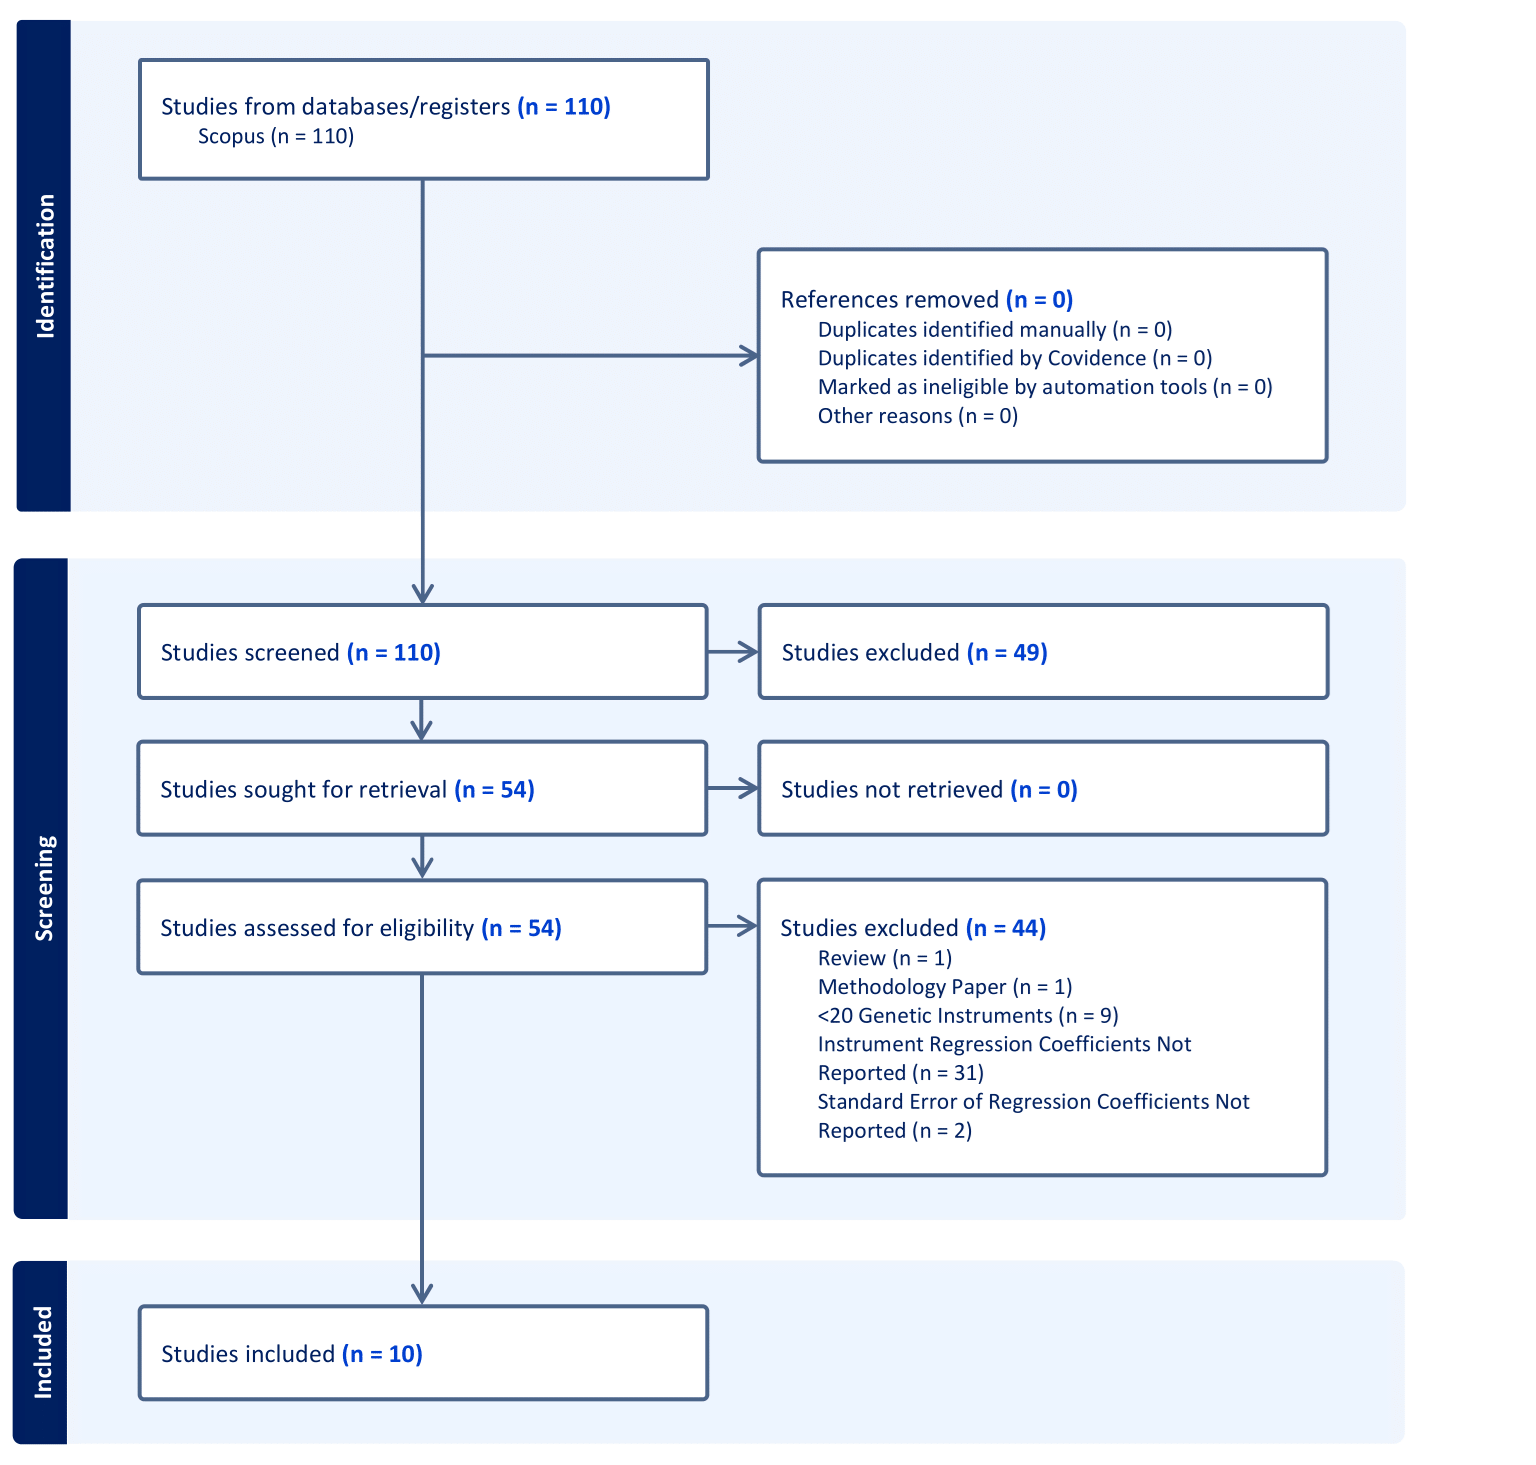
\includegraphics[width=1\linewidth]{Data/Citations_Search/WME_citation_search_flow_diagram_crop} \caption{Flow diagram illustrating selection of sample of ten highly-cited two-sample Mendelian randomisation articles reporting a weighted median estimate of casual effect}\label{fig:screening-flow}
\end{figure}

\begin{landscape}

\global\setlength{\Oldarrayrulewidth}{\arrayrulewidth}

\global\setlength{\Oldtabcolsep}{\tabcolsep}

\setlength{\tabcolsep}{2pt}

\renewcommand*{\arraystretch}{1.3}



\providecommand{\ascline}[3]{\noalign{\global\arrayrulewidth #1}\arrayrulecolor[HTML]{#2}\cline{#3}}

\begin{longtable}[c]{|p{0.75in}|p{0.75in}|p{0.98in}|p{0.75in}|p{0.75in}|p{0.75in}|p{0.75in}|p{0.75in}|p{0.75in}|p{0.75in}|p{0.75in}}

\caption{Summary\ of\ ten\ highly-cited\ two-sample\ Mendelian\ randomisation\ articles\ reporting\ a\ weighted\ median\ estimate\ of\ casual\ effect}\label{tab:citation-search-sample-display}\\

\ascline{1.5pt}{666666}{1-11}

\multicolumn{1}{>{\centering}m{\dimexpr 0.75in+0\tabcolsep}}{} & \multicolumn{1}{>{\centering}m{\dimexpr 0.75in+0\tabcolsep}}{} & \multicolumn{1}{>{\centering}m{\dimexpr 0.98in+0\tabcolsep}}{} & \multicolumn{1}{>{\centering}m{\dimexpr 0.75in+0\tabcolsep}}{} & \multicolumn{3}{>{\centering}m{\dimexpr 2.25in+4\tabcolsep}}{\textcolor[HTML]{000000}{\fontsize{9}{9}\selectfont{\global\setmainfont{Arial}{Participants}}}} & \multicolumn{2}{>{\centering}m{\dimexpr 1.5in+2\tabcolsep}}{\textcolor[HTML]{000000}{\fontsize{9}{9}\selectfont{\global\setmainfont{Arial}{Causal}}}} & \multicolumn{1}{>{\centering}m{\dimexpr 0.75in+0\tabcolsep}}{} & \multicolumn{1}{>{\centering}m{\dimexpr 0.75in+0\tabcolsep}}{} \\

\ascline{1pt}{000000}{5-7}



\multicolumn{1}{>{\centering}m{\dimexpr 0.75in+0\tabcolsep}}{} & \multicolumn{1}{>{\centering}m{\dimexpr 0.75in+0\tabcolsep}}{} & \multicolumn{1}{>{\centering}m{\dimexpr 0.98in+0\tabcolsep}}{} & \multicolumn{1}{>{\centering}m{\dimexpr 0.75in+0\tabcolsep}}{} & \multicolumn{2}{>{\centering}m{\dimexpr 1.5in+2\tabcolsep}}{\textcolor[HTML]{000000}{\fontsize{9}{9}\selectfont{\global\setmainfont{Arial}{\textit{N}}}}} & \multicolumn{1}{>{\centering}m{\dimexpr 0.75in+0\tabcolsep}}{\textcolor[HTML]{000000}{\fontsize{9}{9}\selectfont{\global\setmainfont{Arial}{Maximum}}}} & \multicolumn{2}{>{\centering}m{\dimexpr 1.5in+2\tabcolsep}}{\textcolor[HTML]{000000}{\fontsize{9}{9}\selectfont{\global\setmainfont{Arial}{Effect}}}} & \multicolumn{1}{>{\centering}m{\dimexpr 0.75in+0\tabcolsep}}{} & \multicolumn{1}{>{\centering}m{\dimexpr 0.75in+0\tabcolsep}}{} \\

\ascline{1pt}{000000}{8-9}



\multicolumn{1}{>{\centering}m{\dimexpr 0.75in+0\tabcolsep}}{} & \multicolumn{1}{>{\centering}m{\dimexpr 0.75in+0\tabcolsep}}{} & \multicolumn{1}{>{\centering}m{\dimexpr 0.98in+0\tabcolsep}}{} & \multicolumn{1}{>{\centering}m{\dimexpr 0.75in+0\tabcolsep}}{} & \multicolumn{1}{>{\centering}m{\dimexpr 0.75in+0\tabcolsep}}{} & \multicolumn{1}{>{\centering}m{\dimexpr 0.75in+0\tabcolsep}}{} & \multicolumn{1}{>{\centering}m{\dimexpr 0.75in+0\tabcolsep}}{\textcolor[HTML]{000000}{\fontsize{9}{9}\selectfont{\global\setmainfont{Arial}{Estimated}}}} & \multicolumn{1}{>{\centering}m{\dimexpr 0.75in+0\tabcolsep}}{} & \multicolumn{1}{>{\centering}m{\dimexpr 0.75in+0\tabcolsep}}{} & \multicolumn{1}{>{\centering}m{\dimexpr 0.75in+0\tabcolsep}}{} & \multicolumn{1}{>{\centering}m{\dimexpr 0.75in+0\tabcolsep}}{} \\





\multicolumn{1}{>{\centering}m{\dimexpr 0.75in+0\tabcolsep}}{\multirow[c]{-4}{*}{\parbox{0.75in}{\centering \textcolor[HTML]{000000}{\fontsize{9}{9}\selectfont{\global\setmainfont{Arial}{Author}}}}}} & \multicolumn{1}{>{\centering}m{\dimexpr 0.75in+0\tabcolsep}}{\multirow[c]{-4}{*}{\parbox{0.75in}{\centering \textcolor[HTML]{000000}{\fontsize{9}{9}\selectfont{\global\setmainfont{Arial}{Citations}}}}}} & \multicolumn{1}{>{\centering}m{\dimexpr 0.98in+0\tabcolsep}}{\multirow[c]{-4}{*}{\parbox{0.98in}{\centering \textcolor[HTML]{000000}{\fontsize{9}{9}\selectfont{\global\setmainfont{Arial}{Association}}}}}} & \multicolumn{1}{>{\centering}m{\dimexpr 0.75in+0\tabcolsep}}{\multirow[c]{-4}{*}{\parbox{0.75in}{\centering \textcolor[HTML]{000000}{\fontsize{9}{9}\selectfont{\global\setmainfont{Arial}{\textit{N}}}}\textcolor[HTML]{000000}{\fontsize{9}{9}\selectfont{\global\setmainfont{Arial}{\ }}}\textcolor[HTML]{000000}{\fontsize{9}{9}\selectfont{\global\setmainfont{Arial}{\linebreak }}}\textcolor[HTML]{000000}{\fontsize{9}{9}\selectfont{\global\setmainfont{Arial}{Instruments}}}}}} & \multicolumn{1}{>{\centering}m{\dimexpr 0.75in+0\tabcolsep}}{\multirow[c]{-2}{*}{\parbox{0.75in}{\centering \textcolor[HTML]{000000}{\fontsize{9}{9}\selectfont{\global\setmainfont{Arial}{Exposure}}}}}} & \multicolumn{1}{>{\centering}m{\dimexpr 0.75in+0\tabcolsep}}{\multirow[c]{-2}{*}{\parbox{0.75in}{\centering \textcolor[HTML]{000000}{\fontsize{9}{9}\selectfont{\global\setmainfont{Arial}{Outcome}}}}}} & \multicolumn{1}{>{\centering}m{\dimexpr 0.75in+0\tabcolsep}}{\textcolor[HTML]{000000}{\fontsize{9}{9}\selectfont{\global\setmainfont{Arial}{Overlap}}}} & \multicolumn{1}{>{\centering}m{\dimexpr 0.75in+0\tabcolsep}}{\multirow[c]{-2}{*}{\parbox{0.75in}{\centering \textcolor[HTML]{000000}{\fontsize{9}{9}\selectfont{\global\setmainfont{Arial}{Measure}}}}}} & \multicolumn{1}{>{\centering}m{\dimexpr 0.75in+0\tabcolsep}}{\multirow[c]{-2}{*}{\parbox{0.75in}{\centering \textcolor[HTML]{000000}{\fontsize{9}{9}\selectfont{\global\setmainfont{Arial}{Estimate}}}}}} & \multicolumn{1}{>{\centering}m{\dimexpr 0.75in+0\tabcolsep}}{\multirow[c]{-4}{*}{\parbox{0.75in}{\centering \textcolor[HTML]{000000}{\fontsize{9}{9}\selectfont{\global\setmainfont{Arial}{Causality\ Reported}}}}}} & \multicolumn{1}{>{\centering}m{\dimexpr 0.75in+0\tabcolsep}}{\multirow[c]{-4}{*}{\parbox{0.75in}{\centering \textcolor[HTML]{000000}{\fontsize{9}{9}\selectfont{\global\setmainfont{Arial}{\textit{p}}}}\textcolor[HTML]{000000}{\fontsize{9}{9}\selectfont{\global\setmainfont{Arial}{-value}}}}}} \\

\ascline{1.5pt}{666666}{1-11}\endfirsthead \caption[]{Summary\ of\ ten\ highly-cited\ two-sample\ Mendelian\ randomisation\ articles\ reporting\ a\ weighted\ median\ estimate\ of\ casual\ effect}\label{tab:citation-search-sample-display}\\

\ascline{1.5pt}{666666}{1-11}

\multicolumn{1}{>{\centering}m{\dimexpr 0.75in+0\tabcolsep}}{} & \multicolumn{1}{>{\centering}m{\dimexpr 0.75in+0\tabcolsep}}{} & \multicolumn{1}{>{\centering}m{\dimexpr 0.98in+0\tabcolsep}}{} & \multicolumn{1}{>{\centering}m{\dimexpr 0.75in+0\tabcolsep}}{} & \multicolumn{3}{>{\centering}m{\dimexpr 2.25in+4\tabcolsep}}{\textcolor[HTML]{000000}{\fontsize{9}{9}\selectfont{\global\setmainfont{Arial}{Participants}}}} & \multicolumn{2}{>{\centering}m{\dimexpr 1.5in+2\tabcolsep}}{\textcolor[HTML]{000000}{\fontsize{9}{9}\selectfont{\global\setmainfont{Arial}{Causal}}}} & \multicolumn{1}{>{\centering}m{\dimexpr 0.75in+0\tabcolsep}}{} & \multicolumn{1}{>{\centering}m{\dimexpr 0.75in+0\tabcolsep}}{} \\

\ascline{1pt}{000000}{5-7}



\multicolumn{1}{>{\centering}m{\dimexpr 0.75in+0\tabcolsep}}{} & \multicolumn{1}{>{\centering}m{\dimexpr 0.75in+0\tabcolsep}}{} & \multicolumn{1}{>{\centering}m{\dimexpr 0.98in+0\tabcolsep}}{} & \multicolumn{1}{>{\centering}m{\dimexpr 0.75in+0\tabcolsep}}{} & \multicolumn{2}{>{\centering}m{\dimexpr 1.5in+2\tabcolsep}}{\textcolor[HTML]{000000}{\fontsize{9}{9}\selectfont{\global\setmainfont{Arial}{\textit{N}}}}} & \multicolumn{1}{>{\centering}m{\dimexpr 0.75in+0\tabcolsep}}{\textcolor[HTML]{000000}{\fontsize{9}{9}\selectfont{\global\setmainfont{Arial}{Maximum}}}} & \multicolumn{2}{>{\centering}m{\dimexpr 1.5in+2\tabcolsep}}{\textcolor[HTML]{000000}{\fontsize{9}{9}\selectfont{\global\setmainfont{Arial}{Effect}}}} & \multicolumn{1}{>{\centering}m{\dimexpr 0.75in+0\tabcolsep}}{} & \multicolumn{1}{>{\centering}m{\dimexpr 0.75in+0\tabcolsep}}{} \\

\ascline{1pt}{000000}{8-9}



\multicolumn{1}{>{\centering}m{\dimexpr 0.75in+0\tabcolsep}}{} & \multicolumn{1}{>{\centering}m{\dimexpr 0.75in+0\tabcolsep}}{} & \multicolumn{1}{>{\centering}m{\dimexpr 0.98in+0\tabcolsep}}{} & \multicolumn{1}{>{\centering}m{\dimexpr 0.75in+0\tabcolsep}}{} & \multicolumn{1}{>{\centering}m{\dimexpr 0.75in+0\tabcolsep}}{} & \multicolumn{1}{>{\centering}m{\dimexpr 0.75in+0\tabcolsep}}{} & \multicolumn{1}{>{\centering}m{\dimexpr 0.75in+0\tabcolsep}}{\textcolor[HTML]{000000}{\fontsize{9}{9}\selectfont{\global\setmainfont{Arial}{Estimated}}}} & \multicolumn{1}{>{\centering}m{\dimexpr 0.75in+0\tabcolsep}}{} & \multicolumn{1}{>{\centering}m{\dimexpr 0.75in+0\tabcolsep}}{} & \multicolumn{1}{>{\centering}m{\dimexpr 0.75in+0\tabcolsep}}{} & \multicolumn{1}{>{\centering}m{\dimexpr 0.75in+0\tabcolsep}}{} \\





\multicolumn{1}{>{\centering}m{\dimexpr 0.75in+0\tabcolsep}}{\multirow[c]{-4}{*}{\parbox{0.75in}{\centering \textcolor[HTML]{000000}{\fontsize{9}{9}\selectfont{\global\setmainfont{Arial}{Author}}}}}} & \multicolumn{1}{>{\centering}m{\dimexpr 0.75in+0\tabcolsep}}{\multirow[c]{-4}{*}{\parbox{0.75in}{\centering \textcolor[HTML]{000000}{\fontsize{9}{9}\selectfont{\global\setmainfont{Arial}{Citations}}}}}} & \multicolumn{1}{>{\centering}m{\dimexpr 0.98in+0\tabcolsep}}{\multirow[c]{-4}{*}{\parbox{0.98in}{\centering \textcolor[HTML]{000000}{\fontsize{9}{9}\selectfont{\global\setmainfont{Arial}{Association}}}}}} & \multicolumn{1}{>{\centering}m{\dimexpr 0.75in+0\tabcolsep}}{\multirow[c]{-4}{*}{\parbox{0.75in}{\centering \textcolor[HTML]{000000}{\fontsize{9}{9}\selectfont{\global\setmainfont{Arial}{\textit{N}}}}\textcolor[HTML]{000000}{\fontsize{9}{9}\selectfont{\global\setmainfont{Arial}{\ }}}\textcolor[HTML]{000000}{\fontsize{9}{9}\selectfont{\global\setmainfont{Arial}{\linebreak }}}\textcolor[HTML]{000000}{\fontsize{9}{9}\selectfont{\global\setmainfont{Arial}{Instruments}}}}}} & \multicolumn{1}{>{\centering}m{\dimexpr 0.75in+0\tabcolsep}}{\multirow[c]{-2}{*}{\parbox{0.75in}{\centering \textcolor[HTML]{000000}{\fontsize{9}{9}\selectfont{\global\setmainfont{Arial}{Exposure}}}}}} & \multicolumn{1}{>{\centering}m{\dimexpr 0.75in+0\tabcolsep}}{\multirow[c]{-2}{*}{\parbox{0.75in}{\centering \textcolor[HTML]{000000}{\fontsize{9}{9}\selectfont{\global\setmainfont{Arial}{Outcome}}}}}} & \multicolumn{1}{>{\centering}m{\dimexpr 0.75in+0\tabcolsep}}{\textcolor[HTML]{000000}{\fontsize{9}{9}\selectfont{\global\setmainfont{Arial}{Overlap}}}} & \multicolumn{1}{>{\centering}m{\dimexpr 0.75in+0\tabcolsep}}{\multirow[c]{-2}{*}{\parbox{0.75in}{\centering \textcolor[HTML]{000000}{\fontsize{9}{9}\selectfont{\global\setmainfont{Arial}{Measure}}}}}} & \multicolumn{1}{>{\centering}m{\dimexpr 0.75in+0\tabcolsep}}{\multirow[c]{-2}{*}{\parbox{0.75in}{\centering \textcolor[HTML]{000000}{\fontsize{9}{9}\selectfont{\global\setmainfont{Arial}{Estimate}}}}}} & \multicolumn{1}{>{\centering}m{\dimexpr 0.75in+0\tabcolsep}}{\multirow[c]{-4}{*}{\parbox{0.75in}{\centering \textcolor[HTML]{000000}{\fontsize{9}{9}\selectfont{\global\setmainfont{Arial}{Causality\ Reported}}}}}} & \multicolumn{1}{>{\centering}m{\dimexpr 0.75in+0\tabcolsep}}{\multirow[c]{-4}{*}{\parbox{0.75in}{\centering \textcolor[HTML]{000000}{\fontsize{9}{9}\selectfont{\global\setmainfont{Arial}{\textit{p}}}}\textcolor[HTML]{000000}{\fontsize{9}{9}\selectfont{\global\setmainfont{Arial}{-value}}}}}} \\

\ascline{1.5pt}{666666}{1-11}\endhead



\multicolumn{11}{>{\raggedright}m{\dimexpr 8.48in+20\tabcolsep}}{\textcolor[HTML]{000000}{\fontsize{8}{8}\selectfont{\global\setmainfont{Arial}{β\ and\ OR\ presented\ as:\ estimate\ (95\%\ CI).}}}\textcolor[HTML]{000000}{\fontsize{8}{8}\selectfont{\global\setmainfont{Arial}{\linebreak }}}\textcolor[HTML]{000000}{\fontsize{8}{8}\selectfont{\global\setmainfont{Arial}{β:\ causal\ effect\ estimate,\ CI:\ Confidence\ Interval,\ OR:\ Odds\ Ratio,\ SE:\ Standard\ Error.}}}\textcolor[HTML]{000000}{\fontsize{8}{8}\selectfont{\global\setmainfont{Arial}{\linebreak }}}\textcolor[HTML]{000000}{\fontsize{8}{8}\selectfont{\global\setmainfont{Arial}{BMI:\ body\ mass\ index,\ CRP:\ C-reactive\ protein,\ NAFLD:\ non-alcoholic\ fatty\ liver\ disease,\ T2DM:\ type\ 2\ diabetes\ mellitus}}}} \\

\endlastfoot



\multicolumn{1}{>{\centering}m{\dimexpr 0.75in+0\tabcolsep}}{\textcolor[HTML]{000000}{\fontsize{8}{8}\selectfont{\global\setmainfont{Arial}{Budu-Aggrey\ et\ al,\ 2019}}}} & \multicolumn{1}{>{\centering}m{\dimexpr 0.75in+0\tabcolsep}}{\textcolor[HTML]{000000}{\fontsize{8}{8}\selectfont{\global\setmainfont{Arial}{182}}}} & \multicolumn{1}{>{\centering}m{\dimexpr 0.98in+0\tabcolsep}}{\textcolor[HTML]{000000}{\fontsize{8}{8}\selectfont{\global\setmainfont{Arial}{BMI\ vs\ Psoriasis}}}} & \multicolumn{1}{>{\centering}m{\dimexpr 0.75in+0\tabcolsep}}{\textcolor[HTML]{000000}{\fontsize{8}{8}\selectfont{\global\setmainfont{Arial}{97}}}} & \multicolumn{1}{>{\centering}m{\dimexpr 0.75in+0\tabcolsep}}{\textcolor[HTML]{000000}{\fontsize{8}{8}\selectfont{\global\setmainfont{Arial}{339,224}}}} & \multicolumn{1}{>{\centering}m{\dimexpr 0.75in+0\tabcolsep}}{\textcolor[HTML]{000000}{\fontsize{8}{8}\selectfont{\global\setmainfont{Arial}{12,559}}}} & \multicolumn{1}{>{\centering}m{\dimexpr 0.75in+0\tabcolsep}}{\textcolor[HTML]{000000}{\fontsize{8}{8}\selectfont{\global\setmainfont{Arial}{0\%}}}} & \multicolumn{1}{>{\centering}m{\dimexpr 0.75in+0\tabcolsep}}{\textcolor[HTML]{000000}{\fontsize{8}{8}\selectfont{\global\setmainfont{Arial}{OR}}}} & \multicolumn{1}{>{\centering}m{\dimexpr 0.75in+0\tabcolsep}}{\textcolor[HTML]{000000}{\fontsize{8}{8}\selectfont{\global\setmainfont{Arial}{1.06\ (1\ to\ 1.12)}}}} & \multicolumn{1}{>{\centering}m{\dimexpr 0.75in+0\tabcolsep}}{\textcolor[HTML]{000000}{\fontsize{8}{8}\selectfont{\global\setmainfont{Arial}{No}}}} & \multicolumn{1}{>{\centering}m{\dimexpr 0.75in+0\tabcolsep}}{\textcolor[HTML]{000000}{\fontsize{8}{8}\selectfont{\global\setmainfont{Arial}{-}}}} \\

\ascline{0.2pt}{000000}{1-11}



\multicolumn{1}{>{\centering}m{\dimexpr 0.75in+0\tabcolsep}}{\textcolor[HTML]{000000}{\fontsize{8}{8}\selectfont{\global\setmainfont{Arial}{Carreras-Torres\ et\ al,\ 2017}}}} & \multicolumn{1}{>{\centering}m{\dimexpr 0.75in+0\tabcolsep}}{\textcolor[HTML]{000000}{\fontsize{8}{8}\selectfont{\global\setmainfont{Arial}{200}}}} & \multicolumn{1}{>{\centering}m{\dimexpr 0.98in+0\tabcolsep}}{\textcolor[HTML]{000000}{\fontsize{8}{8}\selectfont{\global\setmainfont{Arial}{Height\ vs\ Pancreatic\ Cancer}}}} & \multicolumn{1}{>{\centering}m{\dimexpr 0.75in+0\tabcolsep}}{\textcolor[HTML]{000000}{\fontsize{8}{8}\selectfont{\global\setmainfont{Arial}{558}}}} & \multicolumn{1}{>{\centering}m{\dimexpr 0.75in+0\tabcolsep}}{\textcolor[HTML]{000000}{\fontsize{8}{8}\selectfont{\global\setmainfont{Arial}{253,288}}}} & \multicolumn{1}{>{\centering}m{\dimexpr 0.75in+0\tabcolsep}}{\textcolor[HTML]{000000}{\fontsize{8}{8}\selectfont{\global\setmainfont{Arial}{15,002}}}} & \multicolumn{1}{>{\centering}m{\dimexpr 0.75in+0\tabcolsep}}{\textcolor[HTML]{000000}{\fontsize{8}{8}\selectfont{\global\setmainfont{Arial}{19\%}}}} & \multicolumn{1}{>{\centering}m{\dimexpr 0.75in+0\tabcolsep}}{\textcolor[HTML]{000000}{\fontsize{8}{8}\selectfont{\global\setmainfont{Arial}{OR}}}} & \multicolumn{1}{>{\centering}m{\dimexpr 0.75in+0\tabcolsep}}{\textcolor[HTML]{000000}{\fontsize{8}{8}\selectfont{\global\setmainfont{Arial}{1.14\ (1\ to\ 1.29)}}}} & \multicolumn{1}{>{\centering}m{\dimexpr 0.75in+0\tabcolsep}}{\textcolor[HTML]{000000}{\fontsize{8}{8}\selectfont{\global\setmainfont{Arial}{No}}}} & \multicolumn{1}{>{\centering}m{\dimexpr 0.75in+0\tabcolsep}}{\textcolor[HTML]{000000}{\fontsize{8}{8}\selectfont{\global\setmainfont{Arial}{0.05}}}} \\

\ascline{0.2pt}{000000}{1-11}



\multicolumn{1}{>{\centering}m{\dimexpr 0.75in+0\tabcolsep}}{\textcolor[HTML]{000000}{\fontsize{8}{8}\selectfont{\global\setmainfont{Arial}{Carter\ et\ al,\ 2019}}}} & \multicolumn{1}{>{\centering}m{\dimexpr 0.75in+0\tabcolsep}}{\textcolor[HTML]{000000}{\fontsize{8}{8}\selectfont{\global\setmainfont{Arial}{199}}}} & \multicolumn{1}{>{\centering}m{\dimexpr 0.98in+0\tabcolsep}}{\textcolor[HTML]{000000}{\fontsize{8}{8}\selectfont{\global\setmainfont{Arial}{Education\ vs\ Coronary\ Disease}}}} & \multicolumn{1}{>{\centering}m{\dimexpr 0.75in+0\tabcolsep}}{\textcolor[HTML]{000000}{\fontsize{8}{8}\selectfont{\global\setmainfont{Arial}{1,267}}}} & \multicolumn{1}{>{\centering}m{\dimexpr 0.75in+0\tabcolsep}}{\textcolor[HTML]{000000}{\fontsize{8}{8}\selectfont{\global\setmainfont{Arial}{766,345}}}} & \multicolumn{1}{>{\centering}m{\dimexpr 0.75in+0\tabcolsep}}{\textcolor[HTML]{000000}{\fontsize{8}{8}\selectfont{\global\setmainfont{Arial}{184,305}}}} & \multicolumn{1}{>{\centering}m{\dimexpr 0.75in+0\tabcolsep}}{\textcolor[HTML]{000000}{\fontsize{8}{8}\selectfont{\global\setmainfont{Arial}{0\%}}}} & \multicolumn{1}{>{\centering}m{\dimexpr 0.75in+0\tabcolsep}}{\textcolor[HTML]{000000}{\fontsize{8}{8}\selectfont{\global\setmainfont{Arial}{OR}}}} & \multicolumn{1}{>{\centering}m{\dimexpr 0.75in+0\tabcolsep}}{\textcolor[HTML]{000000}{\fontsize{8}{8}\selectfont{\global\setmainfont{Arial}{0.62\ (0.57\ to\ 0.67)}}}} & \multicolumn{1}{>{\centering}m{\dimexpr 0.75in+0\tabcolsep}}{\textcolor[HTML]{000000}{\fontsize{8}{8}\selectfont{\global\setmainfont{Arial}{Yes}}}} & \multicolumn{1}{>{\centering}m{\dimexpr 0.75in+0\tabcolsep}}{\textcolor[HTML]{000000}{\fontsize{8}{8}\selectfont{\global\setmainfont{Arial}{<0.001}}}} \\

\ascline{0.2pt}{000000}{1-11}



\multicolumn{1}{>{\centering}m{\dimexpr 0.75in+0\tabcolsep}}{\textcolor[HTML]{000000}{\fontsize{8}{8}\selectfont{\global\setmainfont{Arial}{Choi\ et\ al,\ 2019}}}} & \multicolumn{1}{>{\centering}m{\dimexpr 0.75in+0\tabcolsep}}{\textcolor[HTML]{000000}{\fontsize{8}{8}\selectfont{\global\setmainfont{Arial}{492}}}} & \multicolumn{1}{>{\centering}m{\dimexpr 0.98in+0\tabcolsep}}{\textcolor[HTML]{000000}{\fontsize{8}{8}\selectfont{\global\setmainfont{Arial}{Activity\ vs\ Depression}}}} & \multicolumn{1}{>{\centering}m{\dimexpr 0.75in+0\tabcolsep}}{\textcolor[HTML]{000000}{\fontsize{8}{8}\selectfont{\global\setmainfont{Arial}{24}}}} & \multicolumn{1}{>{\centering}m{\dimexpr 0.75in+0\tabcolsep}}{\textcolor[HTML]{000000}{\fontsize{8}{8}\selectfont{\global\setmainfont{Arial}{377,234}}}} & \multicolumn{1}{>{\centering}m{\dimexpr 0.75in+0\tabcolsep}}{\textcolor[HTML]{000000}{\fontsize{8}{8}\selectfont{\global\setmainfont{Arial}{143,265}}}} & \multicolumn{1}{>{\centering}m{\dimexpr 0.75in+0\tabcolsep}}{\textcolor[HTML]{000000}{\fontsize{8}{8}\selectfont{\global\setmainfont{Arial}{0\%}}}} & \multicolumn{1}{>{\centering}m{\dimexpr 0.75in+0\tabcolsep}}{\textcolor[HTML]{000000}{\fontsize{8}{8}\selectfont{\global\setmainfont{Arial}{OR}}}} & \multicolumn{1}{>{\centering}m{\dimexpr 0.75in+0\tabcolsep}}{\textcolor[HTML]{000000}{\fontsize{8}{8}\selectfont{\global\setmainfont{Arial}{1.49\ (0.94\ to\ 2.36)}}}} & \multicolumn{1}{>{\centering}m{\dimexpr 0.75in+0\tabcolsep}}{\textcolor[HTML]{000000}{\fontsize{8}{8}\selectfont{\global\setmainfont{Arial}{No}}}} & \multicolumn{1}{>{\centering}m{\dimexpr 0.75in+0\tabcolsep}}{\textcolor[HTML]{000000}{\fontsize{8}{8}\selectfont{\global\setmainfont{Arial}{0.08}}}} \\

\ascline{0.2pt}{000000}{1-11}



\multicolumn{1}{>{\centering}m{\dimexpr 0.75in+0\tabcolsep}}{\textcolor[HTML]{000000}{\fontsize{8}{8}\selectfont{\global\setmainfont{Arial}{Clift\ et\ al,\ 2022}}}} & \multicolumn{1}{>{\centering}m{\dimexpr 0.75in+0\tabcolsep}}{\textcolor[HTML]{000000}{\fontsize{8}{8}\selectfont{\global\setmainfont{Arial}{129}}}} & \multicolumn{1}{>{\centering}m{\dimexpr 0.98in+0\tabcolsep}}{\textcolor[HTML]{000000}{\fontsize{8}{8}\selectfont{\global\setmainfont{Arial}{Smoking\ Initiation\ vs\ COVID-19\ Infection}}}} & \multicolumn{1}{>{\centering}m{\dimexpr 0.75in+0\tabcolsep}}{\textcolor[HTML]{000000}{\fontsize{8}{8}\selectfont{\global\setmainfont{Arial}{378}}}} & \multicolumn{1}{>{\centering}m{\dimexpr 0.75in+0\tabcolsep}}{\textcolor[HTML]{000000}{\fontsize{8}{8}\selectfont{\global\setmainfont{Arial}{1,232,091}}}} & \multicolumn{1}{>{\centering}m{\dimexpr 0.75in+0\tabcolsep}}{\textcolor[HTML]{000000}{\fontsize{8}{8}\selectfont{\global\setmainfont{Arial}{281,105}}}} & \multicolumn{1}{>{\centering}m{\dimexpr 0.75in+0\tabcolsep}}{\textcolor[HTML]{000000}{\fontsize{8}{8}\selectfont{\global\setmainfont{Arial}{36\%}}}} & \multicolumn{1}{>{\centering}m{\dimexpr 0.75in+0\tabcolsep}}{\textcolor[HTML]{000000}{\fontsize{8}{8}\selectfont{\global\setmainfont{Arial}{OR}}}} & \multicolumn{1}{>{\centering}m{\dimexpr 0.75in+0\tabcolsep}}{\textcolor[HTML]{000000}{\fontsize{8}{8}\selectfont{\global\setmainfont{Arial}{1.53\ (1.02\ to\ 2.28)}}}} & \multicolumn{1}{>{\centering}m{\dimexpr 0.75in+0\tabcolsep}}{\textcolor[HTML]{000000}{\fontsize{8}{8}\selectfont{\global\setmainfont{Arial}{Yes}}}} & \multicolumn{1}{>{\centering}m{\dimexpr 0.75in+0\tabcolsep}}{\textcolor[HTML]{000000}{\fontsize{8}{8}\selectfont{\global\setmainfont{Arial}{0.04}}}} \\

\ascline{0.2pt}{000000}{1-11}



\multicolumn{1}{>{\centering}m{\dimexpr 0.75in+0\tabcolsep}}{\textcolor[HTML]{000000}{\fontsize{8}{8}\selectfont{\global\setmainfont{Arial}{Ligthart\ et\ al,\ 2018}}}} & \multicolumn{1}{>{\centering}m{\dimexpr 0.75in+0\tabcolsep}}{\textcolor[HTML]{000000}{\fontsize{8}{8}\selectfont{\global\setmainfont{Arial}{298}}}} & \multicolumn{1}{>{\centering}m{\dimexpr 0.98in+0\tabcolsep}}{\textcolor[HTML]{000000}{\fontsize{8}{8}\selectfont{\global\setmainfont{Arial}{CRP\ vs\ Schizophrenia}}}} & \multicolumn{1}{>{\centering}m{\dimexpr 0.75in+0\tabcolsep}}{\textcolor[HTML]{000000}{\fontsize{8}{8}\selectfont{\global\setmainfont{Arial}{52}}}} & \multicolumn{1}{>{\centering}m{\dimexpr 0.75in+0\tabcolsep}}{\textcolor[HTML]{000000}{\fontsize{8}{8}\selectfont{\global\setmainfont{Arial}{204,402}}}} & \multicolumn{1}{>{\centering}m{\dimexpr 0.75in+0\tabcolsep}}{\textcolor[HTML]{000000}{\fontsize{8}{8}\selectfont{\global\setmainfont{Arial}{82,315}}}} & \multicolumn{1}{>{\centering}m{\dimexpr 0.75in+0\tabcolsep}}{\textcolor[HTML]{000000}{\fontsize{8}{8}\selectfont{\global\setmainfont{Arial}{0\%}}}} & \multicolumn{1}{>{\centering}m{\dimexpr 0.75in+0\tabcolsep}}{\textcolor[HTML]{000000}{\fontsize{8}{8}\selectfont{\global\setmainfont{Arial}{OR}}}} & \multicolumn{1}{>{\centering}m{\dimexpr 0.75in+0\tabcolsep}}{\textcolor[HTML]{000000}{\fontsize{8}{8}\selectfont{\global\setmainfont{Arial}{0.89\ (0.81\ to\ 0.96)}}}} & \multicolumn{1}{>{\centering}m{\dimexpr 0.75in+0\tabcolsep}}{\textcolor[HTML]{000000}{\fontsize{8}{8}\selectfont{\global\setmainfont{Arial}{Yes}}}} & \multicolumn{1}{>{\centering}m{\dimexpr 0.75in+0\tabcolsep}}{\textcolor[HTML]{000000}{\fontsize{8}{8}\selectfont{\global\setmainfont{Arial}{0.004}}}} \\

\ascline{0.2pt}{000000}{1-11}



\multicolumn{1}{>{\centering}m{\dimexpr 0.75in+0\tabcolsep}}{\textcolor[HTML]{000000}{\fontsize{8}{8}\selectfont{\global\setmainfont{Arial}{Mokry\ et\ al,\ 2016}}}} & \multicolumn{1}{>{\centering}m{\dimexpr 0.75in+0\tabcolsep}}{\textcolor[HTML]{000000}{\fontsize{8}{8}\selectfont{\global\setmainfont{Arial}{199}}}} & \multicolumn{1}{>{\centering}m{\dimexpr 0.98in+0\tabcolsep}}{\textcolor[HTML]{000000}{\fontsize{8}{8}\selectfont{\global\setmainfont{Arial}{BMI\ vs\ Multiple\ Sclerosis}}}} & \multicolumn{1}{>{\centering}m{\dimexpr 0.75in+0\tabcolsep}}{\textcolor[HTML]{000000}{\fontsize{8}{8}\selectfont{\global\setmainfont{Arial}{70}}}} & \multicolumn{1}{>{\centering}m{\dimexpr 0.75in+0\tabcolsep}}{\textcolor[HTML]{000000}{\fontsize{8}{8}\selectfont{\global\setmainfont{Arial}{322,105}}}} & \multicolumn{1}{>{\centering}m{\dimexpr 0.75in+0\tabcolsep}}{\textcolor[HTML]{000000}{\fontsize{8}{8}\selectfont{\global\setmainfont{Arial}{38,589}}}} & \multicolumn{1}{>{\centering}m{\dimexpr 0.75in+0\tabcolsep}}{\textcolor[HTML]{000000}{\fontsize{8}{8}\selectfont{\global\setmainfont{Arial}{2.5\%}}}} & \multicolumn{1}{>{\centering}m{\dimexpr 0.75in+0\tabcolsep}}{\textcolor[HTML]{000000}{\fontsize{8}{8}\selectfont{\global\setmainfont{Arial}{OR}}}} & \multicolumn{1}{>{\centering}m{\dimexpr 0.75in+0\tabcolsep}}{\textcolor[HTML]{000000}{\fontsize{8}{8}\selectfont{\global\setmainfont{Arial}{1.26\ (0.98\ to\ 1.62)}}}} & \multicolumn{1}{>{\centering}m{\dimexpr 0.75in+0\tabcolsep}}{\textcolor[HTML]{000000}{\fontsize{8}{8}\selectfont{\global\setmainfont{Arial}{No}}}} & \multicolumn{1}{>{\centering}m{\dimexpr 0.75in+0\tabcolsep}}{\textcolor[HTML]{000000}{\fontsize{8}{8}\selectfont{\global\setmainfont{Arial}{0.08}}}} \\

\ascline{0.2pt}{000000}{1-11}



\multicolumn{1}{>{\centering}m{\dimexpr 0.75in+0\tabcolsep}}{\textcolor[HTML]{000000}{\fontsize{8}{8}\selectfont{\global\setmainfont{Arial}{Pasman\ et\ al,\ 2018}}}} & \multicolumn{1}{>{\centering}m{\dimexpr 0.75in+0\tabcolsep}}{\textcolor[HTML]{000000}{\fontsize{8}{8}\selectfont{\global\setmainfont{Arial}{328}}}} & \multicolumn{1}{>{\centering}m{\dimexpr 0.98in+0\tabcolsep}}{\textcolor[HTML]{000000}{\fontsize{8}{8}\selectfont{\global\setmainfont{Arial}{Schizophrenia\ vs\ Cannabis\ Use}}}} & \multicolumn{1}{>{\centering}m{\dimexpr 0.75in+0\tabcolsep}}{\textcolor[HTML]{000000}{\fontsize{8}{8}\selectfont{\global\setmainfont{Arial}{102}}}} & \multicolumn{1}{>{\centering}m{\dimexpr 0.75in+0\tabcolsep}}{\textcolor[HTML]{000000}{\fontsize{8}{8}\selectfont{\global\setmainfont{Arial}{150,064}}}} & \multicolumn{1}{>{\centering}m{\dimexpr 0.75in+0\tabcolsep}}{\textcolor[HTML]{000000}{\fontsize{8}{8}\selectfont{\global\setmainfont{Arial}{184,765}}}} & \multicolumn{1}{>{\centering}m{\dimexpr 0.75in+0\tabcolsep}}{\textcolor[HTML]{000000}{\fontsize{8}{8}\selectfont{\global\setmainfont{Arial}{0\%}}}} & \multicolumn{1}{>{\centering}m{\dimexpr 0.75in+0\tabcolsep}}{\textcolor[HTML]{000000}{\fontsize{8}{8}\selectfont{\global\setmainfont{Arial}{\textit{β}}}}} & \multicolumn{1}{>{\centering}m{\dimexpr 0.75in+0\tabcolsep}}{\textcolor[HTML]{000000}{\fontsize{8}{8}\selectfont{\global\setmainfont{Arial}{0.163\ (0.067\ to\ 0.259)}}}} & \multicolumn{1}{>{\centering}m{\dimexpr 0.75in+0\tabcolsep}}{\textcolor[HTML]{000000}{\fontsize{8}{8}\selectfont{\global\setmainfont{Arial}{Yes}}}} & \multicolumn{1}{>{\centering}m{\dimexpr 0.75in+0\tabcolsep}}{\textcolor[HTML]{000000}{\fontsize{8}{8}\selectfont{\global\setmainfont{Arial}{0.001}}}} \\

\ascline{0.2pt}{000000}{1-11}



\multicolumn{1}{>{\centering}m{\dimexpr 0.75in+0\tabcolsep}}{\textcolor[HTML]{000000}{\fontsize{8}{8}\selectfont{\global\setmainfont{Arial}{Xie\ et\ al,\ 2023}}}} & \multicolumn{1}{>{\centering}m{\dimexpr 0.75in+0\tabcolsep}}{\textcolor[HTML]{000000}{\fontsize{8}{8}\selectfont{\global\setmainfont{Arial}{138}}}} & \multicolumn{1}{>{\centering}m{\dimexpr 0.98in+0\tabcolsep}}{\textcolor[HTML]{000000}{\fontsize{8}{8}\selectfont{\global\setmainfont{Arial}{T2DM\ vs\ NAFLD}}}} & \multicolumn{1}{>{\centering}m{\dimexpr 0.75in+0\tabcolsep}}{\textcolor[HTML]{000000}{\fontsize{8}{8}\selectfont{\global\setmainfont{Arial}{449}}}} & \multicolumn{1}{>{\centering}m{\dimexpr 0.75in+0\tabcolsep}}{\textcolor[HTML]{000000}{\fontsize{8}{8}\selectfont{\global\setmainfont{Arial}{441,016}}}} & \multicolumn{1}{>{\centering}m{\dimexpr 0.75in+0\tabcolsep}}{\textcolor[HTML]{000000}{\fontsize{8}{8}\selectfont{\global\setmainfont{Arial}{218,792}}}} & \multicolumn{1}{>{\centering}m{\dimexpr 0.75in+0\tabcolsep}}{\textcolor[HTML]{000000}{\fontsize{8}{8}\selectfont{\global\setmainfont{Arial}{0\%}}}} & \multicolumn{1}{>{\centering}m{\dimexpr 0.75in+0\tabcolsep}}{\textcolor[HTML]{000000}{\fontsize{8}{8}\selectfont{\global\setmainfont{Arial}{OR}}}} & \multicolumn{1}{>{\centering}m{\dimexpr 0.75in+0\tabcolsep}}{\textcolor[HTML]{000000}{\fontsize{8}{8}\selectfont{\global\setmainfont{Arial}{1.61\ (1.09\ to\ 2.38)}}}} & \multicolumn{1}{>{\centering}m{\dimexpr 0.75in+0\tabcolsep}}{\textcolor[HTML]{000000}{\fontsize{8}{8}\selectfont{\global\setmainfont{Arial}{Yes}}}} & \multicolumn{1}{>{\centering}m{\dimexpr 0.75in+0\tabcolsep}}{\textcolor[HTML]{000000}{\fontsize{8}{8}\selectfont{\global\setmainfont{Arial}{<0.001}}}} \\

\ascline{0.2pt}{000000}{1-11}



\multicolumn{1}{>{\centering}m{\dimexpr 0.75in+0\tabcolsep}}{\textcolor[HTML]{000000}{\fontsize{8}{8}\selectfont{\global\setmainfont{Arial}{Xu\ et\ al,\ 2022}}}} & \multicolumn{1}{>{\centering}m{\dimexpr 0.75in+0\tabcolsep}}{\textcolor[HTML]{000000}{\fontsize{8}{8}\selectfont{\global\setmainfont{Arial}{183}}}} & \multicolumn{1}{>{\centering}m{\dimexpr 0.98in+0\tabcolsep}}{\textcolor[HTML]{000000}{\fontsize{8}{8}\selectfont{\global\setmainfont{Arial}{Coeliac\ vs\ Gut\ Bifidobacterium}}}} & \multicolumn{1}{>{\centering}m{\dimexpr 0.75in+0\tabcolsep}}{\textcolor[HTML]{000000}{\fontsize{8}{8}\selectfont{\global\setmainfont{Arial}{105}}}} & \multicolumn{1}{>{\centering}m{\dimexpr 0.75in+0\tabcolsep}}{\textcolor[HTML]{000000}{\fontsize{8}{8}\selectfont{\global\setmainfont{Arial}{15,283}}}} & \multicolumn{1}{>{\centering}m{\dimexpr 0.75in+0\tabcolsep}}{\textcolor[HTML]{000000}{\fontsize{8}{8}\selectfont{\global\setmainfont{Arial}{24,269}}}} & \multicolumn{1}{>{\centering}m{\dimexpr 0.75in+0\tabcolsep}}{\textcolor[HTML]{000000}{\fontsize{8}{8}\selectfont{\global\setmainfont{Arial}{63\%}}}} & \multicolumn{1}{>{\centering}m{\dimexpr 0.75in+0\tabcolsep}}{\textcolor[HTML]{000000}{\fontsize{8}{8}\selectfont{\global\setmainfont{Arial}{OR}}}} & \multicolumn{1}{>{\centering}m{\dimexpr 0.75in+0\tabcolsep}}{\textcolor[HTML]{000000}{\fontsize{8}{8}\selectfont{\global\setmainfont{Arial}{0.998\ (0.99\ to\ 1.005)}}}} & \multicolumn{1}{>{\centering}m{\dimexpr 0.75in+0\tabcolsep}}{\textcolor[HTML]{000000}{\fontsize{8}{8}\selectfont{\global\setmainfont{Arial}{No}}}} & \multicolumn{1}{>{\centering}m{\dimexpr 0.75in+0\tabcolsep}}{\textcolor[HTML]{000000}{\fontsize{8}{8}\selectfont{\global\setmainfont{Arial}{0.56}}}} \\

\ascline{0.2pt}{000000}{1-11}



\end{longtable}



\arrayrulecolor[HTML]{000000}

\global\setlength{\arrayrulewidth}{\Oldarrayrulewidth}

\global\setlength{\tabcolsep}{\Oldtabcolsep}

\renewcommand*{\arraystretch}{1}

\end{landscape}

\subsubsection{Re-Analysis Results}\label{re-analysis-results}

\paragraph{Data Validation and Re-Analysis}\label{data-validation-and-re-analysis}

\leavevmode\newline There were missing gene-outcome coefficients for three instruments from Xie et al\textsuperscript{\citeproc{ref-xie_associations_2023}{32}}, and one instrument in Clift et al\textsuperscript{\citeproc{ref-clift_smoking_2022}{33}} was reported as having an implausibly large gene-outcome coefficient and standard error (-1243.03 and 19161.64, respectively); these were imputed as the respective mean value per study. Data were otherwise complete as expected per the descriptions in each study manuscript. A summary of the re-analysis results is presented in Table \ref{tab:citations-reanalysis-summ-display}; estimates are presented both as \(\beta\) regression coefficients and \hyperref[acronyms_OR]{odds ratio (OR)}s to aid comparison across studies.

\paragraph{Re-Analysed vs Reported WME Causal Estimates}\label{re-analysed-vs-reported-wme-causal-estimates}

\leavevmode\newline 3 of the \hyperref[acronyms_WME]{WME} estimates generated through re-analysis matched the originally reported estimates poorly (Ligthart et al\textsuperscript{\citeproc{ref-ligthart_genome_2018}{26}}, Carreras-Torres et al\textsuperscript{\citeproc{ref-carreras-torres_role_2017}{29}}, Mokry et al\textsuperscript{\citeproc{ref-mokry_obesity_2016}{28}}), with a \textgreater0.1 difference in re-analysis estimates of \hyperref[acronyms_OR]{OR} versus the values originally reported. Re-analysed \hyperref[acronyms_OR]{OR} upper or lower \hyperref[acronyms_CI]{CI}s were \textgreater0.1 different to reported values for 4 studies (Ligthart et al\textsuperscript{\citeproc{ref-ligthart_genome_2018}{26}}, Carreras-Torres et al\textsuperscript{\citeproc{ref-carreras-torres_role_2017}{29}}, Mokry et al\textsuperscript{\citeproc{ref-mokry_obesity_2016}{28}}, Budu-Aggrey et al\textsuperscript{\citeproc{ref-budu-aggrey_evidence_2019}{31}}). Details of instruments used in re-analysis were re-checked against the relevant manuscripts to confirm accuracy of data used, with no discrepancies found.

Overall, estimates and \hyperref[acronyms_CI]{CI}s from re-analysis of the other 6 studies (Choi et al\textsuperscript{\citeproc{ref-choi_assessment_2019}{24}}, Xie et al\textsuperscript{\citeproc{ref-xie_associations_2023}{32}}, Pasman et al\textsuperscript{\citeproc{ref-pasman_gwas_2018}{25}}, Carter et al\textsuperscript{\citeproc{ref-carter_understanding_2019}{27}}, Clift et al\textsuperscript{\citeproc{ref-clift_smoking_2022}{33}}, Xu et al\textsuperscript{\citeproc{ref-xu_causal_2022}{30}}) appeared comparable to reported values, after accounting for rounding errors from published summary data, and random variation inherent in bootstrap generation of \hyperref[acronyms_CI]{CI}s.

Compared with reported values of \hyperref[acronyms_OR]{OR}s across the 9 studies using them, the mean difference for effect estimates (\hyperref[acronyms_SE]{SE} of estimate) from the re-analysis estimate was 0.03 (0.17). For 95\% \hyperref[acronyms_CI]{CI}s, the mean differences between reported and re-analysed values were 0.07 for the lower bounds and -0.04 for upper bounds, i.e.~reported \hyperref[acronyms_CI]{CI}s were narrower on average than re-analysed \hyperref[acronyms_WME]{WME} \hyperref[acronyms_CI]{CI}s.

Conclusions regarding presence of a causal effect were mostly consistent: reported \hyperref[acronyms_WME]{WME} and re-analysed \hyperref[acronyms_WME]{WME} estimates were discordant in detecting a causal exposure-outcome effect for 2 studies: 1 where a previously reported causal effect was not found (Ligthart et al\textsuperscript{\citeproc{ref-ligthart_genome_2018}{26}}), and 1 where a causal effect was found that had not been reported previously (Mokry et al\textsuperscript{\citeproc{ref-mokry_obesity_2016}{28}}).

\paragraph{Re-Analysed WME vs MR-Hevo Causal Estimates}\label{re-analysed-wme-vs-mr-hevo-causal-estimates}

\leavevmode\newline Causal effect estimates generated by MR-Hevo were \textgreater0.1 different from re-analysed \hyperref[acronyms_WME]{WME} estimates for 2 studies (Choi et al\textsuperscript{\citeproc{ref-choi_assessment_2019}{24}}, Carreras-Torres et al\textsuperscript{\citeproc{ref-carreras-torres_role_2017}{29}}). Compared with \hyperref[acronyms_WME]{WME} values of \hyperref[acronyms_OR]{OR}s across the 9 studies using them, the mean difference for effect estimates (\hyperref[acronyms_SE]{SE} of estimate) from the re-analysis estimate was -0.046 (-0.084). For 95\% \hyperref[acronyms_CI]{CI}s, the mean differences between MR-Hevo and \hyperref[acronyms_WME]{WME} values were -0.044 for the lower bounds and -0.002 for upper bounds, i.e.~MR-Hevo \hyperref[acronyms_CI]{CI}s were wider and slightly shifted in the negative direction on average than \hyperref[acronyms_WME]{WME} values. MR-Hevo \hyperref[acronyms_OR]{OR} upper or lower \hyperref[acronyms_CI]{CI}s were \textgreater0.1 different to \hyperref[acronyms_WME]{WME} values for 6 studies (Choi et al\textsuperscript{\citeproc{ref-choi_assessment_2019}{24}}, Xie et al\textsuperscript{\citeproc{ref-xie_associations_2023}{32}}, Ligthart et al\textsuperscript{\citeproc{ref-ligthart_genome_2018}{26}}, Carreras-Torres et al\textsuperscript{\citeproc{ref-carreras-torres_role_2017}{29}}, Clift et al\textsuperscript{\citeproc{ref-clift_smoking_2022}{33}}, Mokry et al\textsuperscript{\citeproc{ref-mokry_obesity_2016}{28}}).

Overall, estimates and \hyperref[acronyms_CI]{CI}s from MR-Hevo analysis of the other 4 studies (Pasman et al\textsuperscript{\citeproc{ref-pasman_gwas_2018}{25}}, Carter et al\textsuperscript{\citeproc{ref-carter_understanding_2019}{27}}, Budu-Aggrey et al\textsuperscript{\citeproc{ref-budu-aggrey_evidence_2019}{31}}, Xu et al\textsuperscript{\citeproc{ref-xu_causal_2022}{30}}) appeared comparable to re-analysed \hyperref[acronyms_WME]{WME} values.

Conclusions regarding presence of a causal effect were consistent: re-analysed \hyperref[acronyms_WME]{WME} estimates were discordant in detecting a causal exposure-outcome effect in 0 studies versus MR-Hevo, with both reporting a causal effect in the same 5 studies (Xie et al\textsuperscript{\citeproc{ref-xie_associations_2023}{32}}, Pasman et al\textsuperscript{\citeproc{ref-pasman_gwas_2018}{25}}, Carter et al\textsuperscript{\citeproc{ref-carter_understanding_2019}{27}}, Clift et al\textsuperscript{\citeproc{ref-clift_smoking_2022}{33}}, Mokry et al\textsuperscript{\citeproc{ref-mokry_obesity_2016}{28}}).

\begin{landscape}

\global\setlength{\Oldarrayrulewidth}{\arrayrulewidth}

\global\setlength{\Oldtabcolsep}{\tabcolsep}

\setlength{\tabcolsep}{2pt}

\renewcommand*{\arraystretch}{1.5}



\providecommand{\ascline}[3]{\noalign{\global\arrayrulewidth #1}\arrayrulecolor[HTML]{#2}\cline{#3}}

\begin{longtable}[c]{|p{0.83in}|p{1.47in}|p{1.01in}|p{0.36in}|p{0.19in}|p{0.75in}|p{0.36in}|p{0.68in}|p{0.47in}|p{0.19in}|p{0.75in}|p{0.36in}|p{0.68in}|p{0.47in}}

\caption{Re-analysis\ of\ ten\ highly-cited\ two-sample\ Mendelian\ randomisation\ articles\ reporting\ a\ weighted\ median\ estimate\ of\ casual\ effect,\ comparing\ results\ of\ both\ WME\ and\ MR-Hevo\ causal\ effect\ estimation\ methods}\label{tab:citations-reanalysis-summ-display}\\

\ascline{1.5pt}{666666}{1-14}

\multicolumn{4}{>{\centering}m{\dimexpr 3.67in+6\tabcolsep}}{\textcolor[HTML]{000000}{\fontsize{8}{8}\selectfont{\global\setmainfont{Arial}{}}}} & \multicolumn{1}{>{\centering}m{\dimexpr 0.19in+0\tabcolsep}}{} & \multicolumn{4}{>{\centering}m{\dimexpr 2.26in+6\tabcolsep}}{} & \multicolumn{1}{>{\centering}m{\dimexpr 0.19in+0\tabcolsep}}{\textcolor[HTML]{000000}{\fontsize{8}{8}\selectfont{\global\setmainfont{Arial}{}}}} & \multicolumn{4}{>{\centering}m{\dimexpr 2.26in+6\tabcolsep}}{} \\





\multicolumn{1}{>{\centering}m{\dimexpr 0.83in+0\tabcolsep}}{} & \multicolumn{1}{>{\centering}m{\dimexpr 1.47in+0\tabcolsep}}{} & \multicolumn{1}{>{\centering}m{\dimexpr 1.01in+0\tabcolsep}}{} & \multicolumn{1}{>{\centering}m{\dimexpr 0.36in+0\tabcolsep}}{} & \multicolumn{1}{>{\centering}m{\dimexpr 0.19in+0\tabcolsep}}{} & \multicolumn{4}{>{\centering}m{\dimexpr 2.26in+6\tabcolsep}}{\multirow[c]{-2}{*}{\parbox{0.75in}{\centering \textcolor[HTML]{000000}{\fontsize{8}{8}\selectfont{\global\setmainfont{Arial}{Weighted\ Median}}}}}} & \multicolumn{1}{>{\centering}m{\dimexpr 0.19in+0\tabcolsep}}{} & \multicolumn{4}{>{\centering}m{\dimexpr 2.26in+6\tabcolsep}}{\multirow[c]{-2}{*}{\parbox{0.75in}{\centering \textcolor[HTML]{000000}{\fontsize{8}{8}\selectfont{\global\setmainfont{Arial}{MR-Hevo}}}}}} \\

\ascline{1pt}{000000}{6-9}\ascline{1pt}{000000}{11-14}



\multicolumn{1}{>{\centering}m{\dimexpr 0.83in+0\tabcolsep}}{\multirow[c]{-2}{*}{\parbox{0.83in}{\centering \textcolor[HTML]{000000}{\fontsize{8}{8}\selectfont{\global\setmainfont{Arial}{Author}}}}}} & \multicolumn{1}{>{\centering}m{\dimexpr 1.47in+0\tabcolsep}}{\multirow[c]{-2}{*}{\parbox{1.47in}{\centering \textcolor[HTML]{000000}{\fontsize{8}{8}\selectfont{\global\setmainfont{Arial}{Exposure}}}}}} & \multicolumn{1}{>{\centering}m{\dimexpr 1.01in+0\tabcolsep}}{\multirow[c]{-2}{*}{\parbox{1.01in}{\centering \textcolor[HTML]{000000}{\fontsize{8}{8}\selectfont{\global\setmainfont{Arial}{Outcome}}}}}} & \multicolumn{1}{>{\centering}m{\dimexpr 0.36in+0\tabcolsep}}{\multirow[c]{-2}{*}{\parbox{0.36in}{\centering \textcolor[HTML]{000000}{\fontsize{8}{8}\selectfont{\global\setmainfont{Arial}{SNPs}}}}}} & \multicolumn{1}{>{\centering}m{\dimexpr 0.19in+0\tabcolsep}}{\multirow[c]{-3}{*}{\parbox{0.19in}{\centering \textcolor[HTML]{000000}{\fontsize{8}{8}\selectfont{\global\setmainfont{Arial}{}}}}}} & \multicolumn{1}{>{\centering}m{\dimexpr 0.75in+0\tabcolsep}}{\textcolor[HTML]{000000}{\fontsize{8}{8}\selectfont{\global\setmainfont{Arial}{β}}}} & \multicolumn{1}{>{\centering}m{\dimexpr 0.36in+0\tabcolsep}}{\textcolor[HTML]{000000}{\fontsize{8}{8}\selectfont{\global\setmainfont{Arial}{SE}}}} & \multicolumn{1}{>{\centering}m{\dimexpr 0.68in+0\tabcolsep}}{\textcolor[HTML]{000000}{\fontsize{8}{8}\selectfont{\global\setmainfont{Arial}{OR}}}} & \multicolumn{1}{>{\centering}m{\dimexpr 0.47in+0\tabcolsep}}{\textcolor[HTML]{000000}{\fontsize{8}{8}\selectfont{\global\setmainfont{Arial}{Causality}}}\textcolor[HTML]{000000}{\fontsize{8}{8}\selectfont{\global\setmainfont{Arial}{\linebreak }}}\textcolor[HTML]{000000}{\fontsize{8}{8}\selectfont{\global\setmainfont{Arial}{Reported}}}} & \multicolumn{1}{>{\centering}m{\dimexpr 0.19in+0\tabcolsep}}{\multirow[c]{-2}{*}{\parbox{0.19in}{\centering \textcolor[HTML]{000000}{\fontsize{8}{8}\selectfont{\global\setmainfont{Arial}{}}}}}} & \multicolumn{1}{>{\centering}m{\dimexpr 0.75in+0\tabcolsep}}{\textcolor[HTML]{000000}{\fontsize{8}{8}\selectfont{\global\setmainfont{Arial}{β}}}} & \multicolumn{1}{>{\centering}m{\dimexpr 0.36in+0\tabcolsep}}{\textcolor[HTML]{000000}{\fontsize{8}{8}\selectfont{\global\setmainfont{Arial}{SE}}}} & \multicolumn{1}{>{\centering}m{\dimexpr 0.68in+0\tabcolsep}}{\textcolor[HTML]{000000}{\fontsize{8}{8}\selectfont{\global\setmainfont{Arial}{OR}}}} & \multicolumn{1}{>{\centering}m{\dimexpr 0.47in+0\tabcolsep}}{\textcolor[HTML]{000000}{\fontsize{8}{8}\selectfont{\global\setmainfont{Arial}{Causality}}}\textcolor[HTML]{000000}{\fontsize{8}{8}\selectfont{\global\setmainfont{Arial}{\linebreak }}}\textcolor[HTML]{000000}{\fontsize{8}{8}\selectfont{\global\setmainfont{Arial}{Reported}}}} \\

\ascline{1.5pt}{666666}{1-14}\endfirsthead \caption[]{Re-analysis\ of\ ten\ highly-cited\ two-sample\ Mendelian\ randomisation\ articles\ reporting\ a\ weighted\ median\ estimate\ of\ casual\ effect,\ comparing\ results\ of\ both\ WME\ and\ MR-Hevo\ causal\ effect\ estimation\ methods}\label{tab:citations-reanalysis-summ-display}\\

\ascline{1.5pt}{666666}{1-14}

\multicolumn{4}{>{\centering}m{\dimexpr 3.67in+6\tabcolsep}}{\textcolor[HTML]{000000}{\fontsize{8}{8}\selectfont{\global\setmainfont{Arial}{}}}} & \multicolumn{1}{>{\centering}m{\dimexpr 0.19in+0\tabcolsep}}{} & \multicolumn{4}{>{\centering}m{\dimexpr 2.26in+6\tabcolsep}}{} & \multicolumn{1}{>{\centering}m{\dimexpr 0.19in+0\tabcolsep}}{\textcolor[HTML]{000000}{\fontsize{8}{8}\selectfont{\global\setmainfont{Arial}{}}}} & \multicolumn{4}{>{\centering}m{\dimexpr 2.26in+6\tabcolsep}}{} \\





\multicolumn{1}{>{\centering}m{\dimexpr 0.83in+0\tabcolsep}}{} & \multicolumn{1}{>{\centering}m{\dimexpr 1.47in+0\tabcolsep}}{} & \multicolumn{1}{>{\centering}m{\dimexpr 1.01in+0\tabcolsep}}{} & \multicolumn{1}{>{\centering}m{\dimexpr 0.36in+0\tabcolsep}}{} & \multicolumn{1}{>{\centering}m{\dimexpr 0.19in+0\tabcolsep}}{} & \multicolumn{4}{>{\centering}m{\dimexpr 2.26in+6\tabcolsep}}{\multirow[c]{-2}{*}{\parbox{0.75in}{\centering \textcolor[HTML]{000000}{\fontsize{8}{8}\selectfont{\global\setmainfont{Arial}{Weighted\ Median}}}}}} & \multicolumn{1}{>{\centering}m{\dimexpr 0.19in+0\tabcolsep}}{} & \multicolumn{4}{>{\centering}m{\dimexpr 2.26in+6\tabcolsep}}{\multirow[c]{-2}{*}{\parbox{0.75in}{\centering \textcolor[HTML]{000000}{\fontsize{8}{8}\selectfont{\global\setmainfont{Arial}{MR-Hevo}}}}}} \\

\ascline{1pt}{000000}{6-9}\ascline{1pt}{000000}{11-14}



\multicolumn{1}{>{\centering}m{\dimexpr 0.83in+0\tabcolsep}}{\multirow[c]{-2}{*}{\parbox{0.83in}{\centering \textcolor[HTML]{000000}{\fontsize{8}{8}\selectfont{\global\setmainfont{Arial}{Author}}}}}} & \multicolumn{1}{>{\centering}m{\dimexpr 1.47in+0\tabcolsep}}{\multirow[c]{-2}{*}{\parbox{1.47in}{\centering \textcolor[HTML]{000000}{\fontsize{8}{8}\selectfont{\global\setmainfont{Arial}{Exposure}}}}}} & \multicolumn{1}{>{\centering}m{\dimexpr 1.01in+0\tabcolsep}}{\multirow[c]{-2}{*}{\parbox{1.01in}{\centering \textcolor[HTML]{000000}{\fontsize{8}{8}\selectfont{\global\setmainfont{Arial}{Outcome}}}}}} & \multicolumn{1}{>{\centering}m{\dimexpr 0.36in+0\tabcolsep}}{\multirow[c]{-2}{*}{\parbox{0.36in}{\centering \textcolor[HTML]{000000}{\fontsize{8}{8}\selectfont{\global\setmainfont{Arial}{SNPs}}}}}} & \multicolumn{1}{>{\centering}m{\dimexpr 0.19in+0\tabcolsep}}{\multirow[c]{-3}{*}{\parbox{0.19in}{\centering \textcolor[HTML]{000000}{\fontsize{8}{8}\selectfont{\global\setmainfont{Arial}{}}}}}} & \multicolumn{1}{>{\centering}m{\dimexpr 0.75in+0\tabcolsep}}{\textcolor[HTML]{000000}{\fontsize{8}{8}\selectfont{\global\setmainfont{Arial}{β}}}} & \multicolumn{1}{>{\centering}m{\dimexpr 0.36in+0\tabcolsep}}{\textcolor[HTML]{000000}{\fontsize{8}{8}\selectfont{\global\setmainfont{Arial}{SE}}}} & \multicolumn{1}{>{\centering}m{\dimexpr 0.68in+0\tabcolsep}}{\textcolor[HTML]{000000}{\fontsize{8}{8}\selectfont{\global\setmainfont{Arial}{OR}}}} & \multicolumn{1}{>{\centering}m{\dimexpr 0.47in+0\tabcolsep}}{\textcolor[HTML]{000000}{\fontsize{8}{8}\selectfont{\global\setmainfont{Arial}{Causality}}}\textcolor[HTML]{000000}{\fontsize{8}{8}\selectfont{\global\setmainfont{Arial}{\linebreak }}}\textcolor[HTML]{000000}{\fontsize{8}{8}\selectfont{\global\setmainfont{Arial}{Reported}}}} & \multicolumn{1}{>{\centering}m{\dimexpr 0.19in+0\tabcolsep}}{\multirow[c]{-2}{*}{\parbox{0.19in}{\centering \textcolor[HTML]{000000}{\fontsize{8}{8}\selectfont{\global\setmainfont{Arial}{}}}}}} & \multicolumn{1}{>{\centering}m{\dimexpr 0.75in+0\tabcolsep}}{\textcolor[HTML]{000000}{\fontsize{8}{8}\selectfont{\global\setmainfont{Arial}{β}}}} & \multicolumn{1}{>{\centering}m{\dimexpr 0.36in+0\tabcolsep}}{\textcolor[HTML]{000000}{\fontsize{8}{8}\selectfont{\global\setmainfont{Arial}{SE}}}} & \multicolumn{1}{>{\centering}m{\dimexpr 0.68in+0\tabcolsep}}{\textcolor[HTML]{000000}{\fontsize{8}{8}\selectfont{\global\setmainfont{Arial}{OR}}}} & \multicolumn{1}{>{\centering}m{\dimexpr 0.47in+0\tabcolsep}}{\textcolor[HTML]{000000}{\fontsize{8}{8}\selectfont{\global\setmainfont{Arial}{Causality}}}\textcolor[HTML]{000000}{\fontsize{8}{8}\selectfont{\global\setmainfont{Arial}{\linebreak }}}\textcolor[HTML]{000000}{\fontsize{8}{8}\selectfont{\global\setmainfont{Arial}{Reported}}}} \\

\ascline{1.5pt}{666666}{1-14}\endhead



\multicolumn{14}{>{\raggedright}m{\dimexpr 8.56in+26\tabcolsep}}{\textcolor[HTML]{000000}{\fontsize{8}{8}\selectfont{\global\setmainfont{Arial}{β\ and\ OR\ presented\ as:\ estimate\ (95\%\ CI).}}}\textcolor[HTML]{000000}{\fontsize{8}{8}\selectfont{\global\setmainfont{Arial}{\linebreak }}}\textcolor[HTML]{000000}{\fontsize{8}{8}\selectfont{\global\setmainfont{Arial}{β:\ causal\ effect\ estimate,\ CI:\ Confidence\ Interval,\ OR:\ Odds\ Ratio,\ SE:\ Standard\ Error.}}}\textcolor[HTML]{000000}{\fontsize{8}{8}\selectfont{\global\setmainfont{Arial}{\linebreak }}}\textcolor[HTML]{000000}{\fontsize{8}{8}\selectfont{\global\setmainfont{Arial}{BMI:\ body\ mass\ index,\ CRP:\ C-reactive\ protein,\ NAFLD:\ non-alcoholic\ fatty\ liver\ disease,\ T2DM:\ type\ 2\ diabetes\ mellitus}}}} \\

\endlastfoot



\multicolumn{1}{>{\centering}m{\dimexpr 0.83in+0\tabcolsep}}{\textcolor[HTML]{000000}{\fontsize{8}{8}\selectfont{\global\setmainfont{Arial}{Budu-Aggrey\ et\ al}}}} & \multicolumn{1}{>{\centering}m{\dimexpr 1.47in+0\tabcolsep}}{\textcolor[HTML]{000000}{\fontsize{8}{8}\selectfont{\global\setmainfont{Arial}{BMI}}}} & \multicolumn{1}{>{\centering}m{\dimexpr 1.01in+0\tabcolsep}}{\textcolor[HTML]{000000}{\fontsize{8}{8}\selectfont{\global\setmainfont{Arial}{Psoriasis}}}} & \multicolumn{1}{>{\centering}m{\dimexpr 0.36in+0\tabcolsep}}{\textcolor[HTML]{000000}{\fontsize{8}{8}\selectfont{\global\setmainfont{Arial}{97}}}} & \multicolumn{1}{>{\centering}m{\dimexpr 0.19in+0\tabcolsep}}{\textcolor[HTML]{000000}{\fontsize{8}{8}\selectfont{\global\setmainfont{Arial}{}}}} & \multicolumn{1}{>{\centering}m{\dimexpr 0.75in+0\tabcolsep}}{\textcolor[HTML]{000000}{\fontsize{8}{8}\selectfont{\global\setmainfont{Arial}{0\ (-0.29-0.29)}}}} & \multicolumn{1}{>{\centering}m{\dimexpr 0.36in+0\tabcolsep}}{\textcolor[HTML]{000000}{\fontsize{8}{8}\selectfont{\global\setmainfont{Arial}{0.148}}}} & \multicolumn{1}{>{\centering}m{\dimexpr 0.68in+0\tabcolsep}}{\textcolor[HTML]{000000}{\fontsize{8}{8}\selectfont{\global\setmainfont{Arial}{1\ (0.75-1.34)}}}} & \multicolumn{1}{>{\centering}m{\dimexpr 0.47in+0\tabcolsep}}{\textcolor[HTML]{000000}{\fontsize{8}{8}\selectfont{\global\setmainfont{Arial}{No}}}} & \multicolumn{1}{>{\centering}m{\dimexpr 0.19in+0\tabcolsep}}{\textcolor[HTML]{000000}{\fontsize{8}{8}\selectfont{\global\setmainfont{Arial}{}}}} & \multicolumn{1}{>{\centering}m{\dimexpr 0.75in+0\tabcolsep}}{\textcolor[HTML]{000000}{\fontsize{8}{8}\selectfont{\global\setmainfont{Arial}{0.08\ (-0.17-0.33)}}}} & \multicolumn{1}{>{\centering}m{\dimexpr 0.36in+0\tabcolsep}}{\textcolor[HTML]{000000}{\fontsize{8}{8}\selectfont{\global\setmainfont{Arial}{0.002}}}} & \multicolumn{1}{>{\centering}m{\dimexpr 0.68in+0\tabcolsep}}{\textcolor[HTML]{000000}{\fontsize{8}{8}\selectfont{\global\setmainfont{Arial}{1.08\ (0.84-1.39)}}}} & \multicolumn{1}{>{\centering}m{\dimexpr 0.47in+0\tabcolsep}}{\textcolor[HTML]{000000}{\fontsize{8}{8}\selectfont{\global\setmainfont{Arial}{No}}}} \\

\ascline{0.2pt}{000000}{1-14}



\multicolumn{1}{>{\centering}m{\dimexpr 0.83in+0\tabcolsep}}{\textcolor[HTML]{000000}{\fontsize{8}{8}\selectfont{\global\setmainfont{Arial}{Carreras-Torres\ et\ al}}}} & \multicolumn{1}{>{\centering}m{\dimexpr 1.47in+0\tabcolsep}}{\textcolor[HTML]{000000}{\fontsize{8}{8}\selectfont{\global\setmainfont{Arial}{Height}}}} & \multicolumn{1}{>{\centering}m{\dimexpr 1.01in+0\tabcolsep}}{\textcolor[HTML]{000000}{\fontsize{8}{8}\selectfont{\global\setmainfont{Arial}{Pancreatic\ Cancer}}}} & \multicolumn{1}{>{\centering}m{\dimexpr 0.36in+0\tabcolsep}}{\textcolor[HTML]{000000}{\fontsize{8}{8}\selectfont{\global\setmainfont{Arial}{558}}}} & \multicolumn{1}{>{\centering}m{\dimexpr 0.19in+0\tabcolsep}}{\textcolor[HTML]{000000}{\fontsize{8}{8}\selectfont{\global\setmainfont{Arial}{}}}} & \multicolumn{1}{>{\centering}m{\dimexpr 0.75in+0\tabcolsep}}{\textcolor[HTML]{000000}{\fontsize{8}{8}\selectfont{\global\setmainfont{Arial}{0\ (-0.13-0.13)}}}} & \multicolumn{1}{>{\centering}m{\dimexpr 0.36in+0\tabcolsep}}{\textcolor[HTML]{000000}{\fontsize{8}{8}\selectfont{\global\setmainfont{Arial}{0.066}}}} & \multicolumn{1}{>{\centering}m{\dimexpr 0.68in+0\tabcolsep}}{\textcolor[HTML]{000000}{\fontsize{8}{8}\selectfont{\global\setmainfont{Arial}{1\ (0.88-1.14)}}}} & \multicolumn{1}{>{\centering}m{\dimexpr 0.47in+0\tabcolsep}}{\textcolor[HTML]{000000}{\fontsize{8}{8}\selectfont{\global\setmainfont{Arial}{No}}}} & \multicolumn{1}{>{\centering}m{\dimexpr 0.19in+0\tabcolsep}}{\textcolor[HTML]{000000}{\fontsize{8}{8}\selectfont{\global\setmainfont{Arial}{}}}} & \multicolumn{1}{>{\centering}m{\dimexpr 0.75in+0\tabcolsep}}{\textcolor[HTML]{000000}{\fontsize{8}{8}\selectfont{\global\setmainfont{Arial}{-0.28\ (-1.34-0.5)}}}} & \multicolumn{1}{>{\centering}m{\dimexpr 0.36in+0\tabcolsep}}{\textcolor[HTML]{000000}{\fontsize{8}{8}\selectfont{\global\setmainfont{Arial}{0.513}}}} & \multicolumn{1}{>{\centering}m{\dimexpr 0.68in+0\tabcolsep}}{\textcolor[HTML]{000000}{\fontsize{8}{8}\selectfont{\global\setmainfont{Arial}{0.76\ (0.26-1.64)}}}} & \multicolumn{1}{>{\centering}m{\dimexpr 0.47in+0\tabcolsep}}{\textcolor[HTML]{000000}{\fontsize{8}{8}\selectfont{\global\setmainfont{Arial}{No}}}} \\

\ascline{0.2pt}{000000}{1-14}



\multicolumn{1}{>{\centering}m{\dimexpr 0.83in+0\tabcolsep}}{\textcolor[HTML]{000000}{\fontsize{8}{8}\selectfont{\global\setmainfont{Arial}{Carter\ et\ al}}}} & \multicolumn{1}{>{\centering}m{\dimexpr 1.47in+0\tabcolsep}}{\textcolor[HTML]{000000}{\fontsize{8}{8}\selectfont{\global\setmainfont{Arial}{Years\ of\ Education}}}} & \multicolumn{1}{>{\centering}m{\dimexpr 1.01in+0\tabcolsep}}{\textcolor[HTML]{000000}{\fontsize{8}{8}\selectfont{\global\setmainfont{Arial}{Coronary\ Artery\ Disease}}}} & \multicolumn{1}{>{\centering}m{\dimexpr 0.36in+0\tabcolsep}}{\textcolor[HTML]{000000}{\fontsize{8}{8}\selectfont{\global\setmainfont{Arial}{1,266}}}} & \multicolumn{1}{>{\centering}m{\dimexpr 0.19in+0\tabcolsep}}{\textcolor[HTML]{000000}{\fontsize{8}{8}\selectfont{\global\setmainfont{Arial}{}}}} & \multicolumn{1}{>{\centering}m{\dimexpr 0.75in+0\tabcolsep}}{\textcolor[HTML]{000000}{\fontsize{8}{8}\selectfont{\global\setmainfont{Arial}{-0.46\ (-0.55--0.38)}}}} & \multicolumn{1}{>{\centering}m{\dimexpr 0.36in+0\tabcolsep}}{\textcolor[HTML]{000000}{\fontsize{8}{8}\selectfont{\global\setmainfont{Arial}{0.044}}}} & \multicolumn{1}{>{\centering}m{\dimexpr 0.68in+0\tabcolsep}}{\textcolor[HTML]{000000}{\fontsize{8}{8}\selectfont{\global\setmainfont{Arial}{0.63\ (0.58-0.69)}}}} & \multicolumn{1}{>{\centering}m{\dimexpr 0.47in+0\tabcolsep}}{\textcolor[HTML]{000000}{\fontsize{8}{8}\selectfont{\global\setmainfont{Arial}{Yes}}}} & \multicolumn{1}{>{\centering}m{\dimexpr 0.19in+0\tabcolsep}}{\textcolor[HTML]{000000}{\fontsize{8}{8}\selectfont{\global\setmainfont{Arial}{}}}} & \multicolumn{1}{>{\centering}m{\dimexpr 0.75in+0\tabcolsep}}{\textcolor[HTML]{000000}{\fontsize{8}{8}\selectfont{\global\setmainfont{Arial}{-0.48\ (-0.54--0.42)}}}} & \multicolumn{1}{>{\centering}m{\dimexpr 0.36in+0\tabcolsep}}{\textcolor[HTML]{000000}{\fontsize{8}{8}\selectfont{\global\setmainfont{Arial}{0.000}}}} & \multicolumn{1}{>{\centering}m{\dimexpr 0.68in+0\tabcolsep}}{\textcolor[HTML]{000000}{\fontsize{8}{8}\selectfont{\global\setmainfont{Arial}{0.62\ (0.58-0.66)}}}} & \multicolumn{1}{>{\centering}m{\dimexpr 0.47in+0\tabcolsep}}{\textcolor[HTML]{000000}{\fontsize{8}{8}\selectfont{\global\setmainfont{Arial}{Yes}}}} \\

\ascline{0.2pt}{000000}{1-14}



\multicolumn{1}{>{\centering}m{\dimexpr 0.83in+0\tabcolsep}}{\textcolor[HTML]{000000}{\fontsize{8}{8}\selectfont{\global\setmainfont{Arial}{Choi\ et\ al}}}} & \multicolumn{1}{>{\centering}m{\dimexpr 1.47in+0\tabcolsep}}{\textcolor[HTML]{000000}{\fontsize{8}{8}\selectfont{\global\setmainfont{Arial}{Self-Reported\ Physical\ Activity}}}} & \multicolumn{1}{>{\centering}m{\dimexpr 1.01in+0\tabcolsep}}{\textcolor[HTML]{000000}{\fontsize{8}{8}\selectfont{\global\setmainfont{Arial}{Major\ Depressive\ Disorder}}}} & \multicolumn{1}{>{\centering}m{\dimexpr 0.36in+0\tabcolsep}}{\textcolor[HTML]{000000}{\fontsize{8}{8}\selectfont{\global\setmainfont{Arial}{25}}}} & \multicolumn{1}{>{\centering}m{\dimexpr 0.19in+0\tabcolsep}}{\textcolor[HTML]{000000}{\fontsize{8}{8}\selectfont{\global\setmainfont{Arial}{}}}} & \multicolumn{1}{>{\centering}m{\dimexpr 0.75in+0\tabcolsep}}{\textcolor[HTML]{000000}{\fontsize{8}{8}\selectfont{\global\setmainfont{Arial}{0.39\ (-0.06-0.83)}}}} & \multicolumn{1}{>{\centering}m{\dimexpr 0.36in+0\tabcolsep}}{\textcolor[HTML]{000000}{\fontsize{8}{8}\selectfont{\global\setmainfont{Arial}{0.227}}}} & \multicolumn{1}{>{\centering}m{\dimexpr 0.68in+0\tabcolsep}}{\textcolor[HTML]{000000}{\fontsize{8}{8}\selectfont{\global\setmainfont{Arial}{1.47\ (0.94-2.29)}}}} & \multicolumn{1}{>{\centering}m{\dimexpr 0.47in+0\tabcolsep}}{\textcolor[HTML]{000000}{\fontsize{8}{8}\selectfont{\global\setmainfont{Arial}{No}}}} & \multicolumn{1}{>{\centering}m{\dimexpr 0.19in+0\tabcolsep}}{\textcolor[HTML]{000000}{\fontsize{8}{8}\selectfont{\global\setmainfont{Arial}{}}}} & \multicolumn{1}{>{\centering}m{\dimexpr 0.75in+0\tabcolsep}}{\textcolor[HTML]{000000}{\fontsize{8}{8}\selectfont{\global\setmainfont{Arial}{0.22\ (-0.23-0.65)}}}} & \multicolumn{1}{>{\centering}m{\dimexpr 0.36in+0\tabcolsep}}{\textcolor[HTML]{000000}{\fontsize{8}{8}\selectfont{\global\setmainfont{Arial}{0.004}}}} & \multicolumn{1}{>{\centering}m{\dimexpr 0.68in+0\tabcolsep}}{\textcolor[HTML]{000000}{\fontsize{8}{8}\selectfont{\global\setmainfont{Arial}{1.25\ (0.8-1.91)}}}} & \multicolumn{1}{>{\centering}m{\dimexpr 0.47in+0\tabcolsep}}{\textcolor[HTML]{000000}{\fontsize{8}{8}\selectfont{\global\setmainfont{Arial}{No}}}} \\

\ascline{0.2pt}{000000}{1-14}



\multicolumn{1}{>{\centering}m{\dimexpr 0.83in+0\tabcolsep}}{\textcolor[HTML]{000000}{\fontsize{8}{8}\selectfont{\global\setmainfont{Arial}{Clift\ et\ al}}}} & \multicolumn{1}{>{\centering}m{\dimexpr 1.47in+0\tabcolsep}}{\textcolor[HTML]{000000}{\fontsize{8}{8}\selectfont{\global\setmainfont{Arial}{Genetically\ Determined\ Smoking\ Initiation}}}} & \multicolumn{1}{>{\centering}m{\dimexpr 1.01in+0\tabcolsep}}{\textcolor[HTML]{000000}{\fontsize{8}{8}\selectfont{\global\setmainfont{Arial}{COVID-19\ Infection}}}} & \multicolumn{1}{>{\centering}m{\dimexpr 0.36in+0\tabcolsep}}{\textcolor[HTML]{000000}{\fontsize{8}{8}\selectfont{\global\setmainfont{Arial}{378}}}} & \multicolumn{1}{>{\centering}m{\dimexpr 0.19in+0\tabcolsep}}{\textcolor[HTML]{000000}{\fontsize{8}{8}\selectfont{\global\setmainfont{Arial}{}}}} & \multicolumn{1}{>{\centering}m{\dimexpr 0.75in+0\tabcolsep}}{\textcolor[HTML]{000000}{\fontsize{8}{8}\selectfont{\global\setmainfont{Arial}{0.43\ (0.02-0.84)}}}} & \multicolumn{1}{>{\centering}m{\dimexpr 0.36in+0\tabcolsep}}{\textcolor[HTML]{000000}{\fontsize{8}{8}\selectfont{\global\setmainfont{Arial}{0.209}}}} & \multicolumn{1}{>{\centering}m{\dimexpr 0.68in+0\tabcolsep}}{\textcolor[HTML]{000000}{\fontsize{8}{8}\selectfont{\global\setmainfont{Arial}{1.53\ (1.02-2.31)}}}} & \multicolumn{1}{>{\centering}m{\dimexpr 0.47in+0\tabcolsep}}{\textcolor[HTML]{000000}{\fontsize{8}{8}\selectfont{\global\setmainfont{Arial}{Yes}}}} & \multicolumn{1}{>{\centering}m{\dimexpr 0.19in+0\tabcolsep}}{\textcolor[HTML]{000000}{\fontsize{8}{8}\selectfont{\global\setmainfont{Arial}{}}}} & \multicolumn{1}{>{\centering}m{\dimexpr 0.75in+0\tabcolsep}}{\textcolor[HTML]{000000}{\fontsize{8}{8}\selectfont{\global\setmainfont{Arial}{0.37\ (0.1-0.64)}}}} & \multicolumn{1}{>{\centering}m{\dimexpr 0.36in+0\tabcolsep}}{\textcolor[HTML]{000000}{\fontsize{8}{8}\selectfont{\global\setmainfont{Arial}{0.001}}}} & \multicolumn{1}{>{\centering}m{\dimexpr 0.68in+0\tabcolsep}}{\textcolor[HTML]{000000}{\fontsize{8}{8}\selectfont{\global\setmainfont{Arial}{1.45\ (1.1-1.9)}}}} & \multicolumn{1}{>{\centering}m{\dimexpr 0.47in+0\tabcolsep}}{\textcolor[HTML]{000000}{\fontsize{8}{8}\selectfont{\global\setmainfont{Arial}{Yes}}}} \\

\ascline{0.2pt}{000000}{1-14}



\multicolumn{1}{>{\centering}m{\dimexpr 0.83in+0\tabcolsep}}{\textcolor[HTML]{000000}{\fontsize{8}{8}\selectfont{\global\setmainfont{Arial}{Ligthart\ et\ al}}}} & \multicolumn{1}{>{\centering}m{\dimexpr 1.47in+0\tabcolsep}}{\textcolor[HTML]{000000}{\fontsize{8}{8}\selectfont{\global\setmainfont{Arial}{Genetically\ Determined\ CRP}}}} & \multicolumn{1}{>{\centering}m{\dimexpr 1.01in+0\tabcolsep}}{\textcolor[HTML]{000000}{\fontsize{8}{8}\selectfont{\global\setmainfont{Arial}{Schizophrenia}}}} & \multicolumn{1}{>{\centering}m{\dimexpr 0.36in+0\tabcolsep}}{\textcolor[HTML]{000000}{\fontsize{8}{8}\selectfont{\global\setmainfont{Arial}{29}}}} & \multicolumn{1}{>{\centering}m{\dimexpr 0.19in+0\tabcolsep}}{\textcolor[HTML]{000000}{\fontsize{8}{8}\selectfont{\global\setmainfont{Arial}{}}}} & \multicolumn{1}{>{\centering}m{\dimexpr 0.75in+0\tabcolsep}}{\textcolor[HTML]{000000}{\fontsize{8}{8}\selectfont{\global\setmainfont{Arial}{-0.41\ (-0.88-0.08)}}}} & \multicolumn{1}{>{\centering}m{\dimexpr 0.36in+0\tabcolsep}}{\textcolor[HTML]{000000}{\fontsize{8}{8}\selectfont{\global\setmainfont{Arial}{0.245}}}} & \multicolumn{1}{>{\centering}m{\dimexpr 0.68in+0\tabcolsep}}{\textcolor[HTML]{000000}{\fontsize{8}{8}\selectfont{\global\setmainfont{Arial}{0.67\ (0.41-1.08)}}}} & \multicolumn{1}{>{\centering}m{\dimexpr 0.47in+0\tabcolsep}}{\textcolor[HTML]{000000}{\fontsize{8}{8}\selectfont{\global\setmainfont{Arial}{No}}}} & \multicolumn{1}{>{\centering}m{\dimexpr 0.19in+0\tabcolsep}}{\textcolor[HTML]{000000}{\fontsize{8}{8}\selectfont{\global\setmainfont{Arial}{}}}} & \multicolumn{1}{>{\centering}m{\dimexpr 0.75in+0\tabcolsep}}{\textcolor[HTML]{000000}{\fontsize{8}{8}\selectfont{\global\setmainfont{Arial}{-0.38\ (-1.24-0.54)}}}} & \multicolumn{1}{>{\centering}m{\dimexpr 0.36in+0\tabcolsep}}{\textcolor[HTML]{000000}{\fontsize{8}{8}\selectfont{\global\setmainfont{Arial}{0.008}}}} & \multicolumn{1}{>{\centering}m{\dimexpr 0.68in+0\tabcolsep}}{\textcolor[HTML]{000000}{\fontsize{8}{8}\selectfont{\global\setmainfont{Arial}{0.68\ (0.29-1.72)}}}} & \multicolumn{1}{>{\centering}m{\dimexpr 0.47in+0\tabcolsep}}{\textcolor[HTML]{000000}{\fontsize{8}{8}\selectfont{\global\setmainfont{Arial}{No}}}} \\

\ascline{0.2pt}{000000}{1-14}



\multicolumn{1}{>{\centering}m{\dimexpr 0.83in+0\tabcolsep}}{\textcolor[HTML]{000000}{\fontsize{8}{8}\selectfont{\global\setmainfont{Arial}{Mokry\ et\ al}}}} & \multicolumn{1}{>{\centering}m{\dimexpr 1.47in+0\tabcolsep}}{\textcolor[HTML]{000000}{\fontsize{8}{8}\selectfont{\global\setmainfont{Arial}{BMI}}}} & \multicolumn{1}{>{\centering}m{\dimexpr 1.01in+0\tabcolsep}}{\textcolor[HTML]{000000}{\fontsize{8}{8}\selectfont{\global\setmainfont{Arial}{Multiple\ Sclerosis}}}} & \multicolumn{1}{>{\centering}m{\dimexpr 0.36in+0\tabcolsep}}{\textcolor[HTML]{000000}{\fontsize{8}{8}\selectfont{\global\setmainfont{Arial}{70}}}} & \multicolumn{1}{>{\centering}m{\dimexpr 0.19in+0\tabcolsep}}{\textcolor[HTML]{000000}{\fontsize{8}{8}\selectfont{\global\setmainfont{Arial}{}}}} & \multicolumn{1}{>{\centering}m{\dimexpr 0.75in+0\tabcolsep}}{\textcolor[HTML]{000000}{\fontsize{8}{8}\selectfont{\global\setmainfont{Arial}{0.34\ (0.09-0.59)}}}} & \multicolumn{1}{>{\centering}m{\dimexpr 0.36in+0\tabcolsep}}{\textcolor[HTML]{000000}{\fontsize{8}{8}\selectfont{\global\setmainfont{Arial}{0.129}}}} & \multicolumn{1}{>{\centering}m{\dimexpr 0.68in+0\tabcolsep}}{\textcolor[HTML]{000000}{\fontsize{8}{8}\selectfont{\global\setmainfont{Arial}{1.41\ (1.09-1.81)}}}} & \multicolumn{1}{>{\centering}m{\dimexpr 0.47in+0\tabcolsep}}{\textcolor[HTML]{000000}{\fontsize{8}{8}\selectfont{\global\setmainfont{Arial}{Yes}}}} & \multicolumn{1}{>{\centering}m{\dimexpr 0.19in+0\tabcolsep}}{\textcolor[HTML]{000000}{\fontsize{8}{8}\selectfont{\global\setmainfont{Arial}{}}}} & \multicolumn{1}{>{\centering}m{\dimexpr 0.75in+0\tabcolsep}}{\textcolor[HTML]{000000}{\fontsize{8}{8}\selectfont{\global\setmainfont{Arial}{0.34\ (0.16-0.52)}}}} & \multicolumn{1}{>{\centering}m{\dimexpr 0.36in+0\tabcolsep}}{\textcolor[HTML]{000000}{\fontsize{8}{8}\selectfont{\global\setmainfont{Arial}{0.001}}}} & \multicolumn{1}{>{\centering}m{\dimexpr 0.68in+0\tabcolsep}}{\textcolor[HTML]{000000}{\fontsize{8}{8}\selectfont{\global\setmainfont{Arial}{1.41\ (1.17-1.67)}}}} & \multicolumn{1}{>{\centering}m{\dimexpr 0.47in+0\tabcolsep}}{\textcolor[HTML]{000000}{\fontsize{8}{8}\selectfont{\global\setmainfont{Arial}{Yes}}}} \\

\ascline{0.2pt}{000000}{1-14}



\multicolumn{1}{>{\centering}m{\dimexpr 0.83in+0\tabcolsep}}{\textcolor[HTML]{000000}{\fontsize{8}{8}\selectfont{\global\setmainfont{Arial}{Pasman\ et\ al}}}} & \multicolumn{1}{>{\centering}m{\dimexpr 1.47in+0\tabcolsep}}{\textcolor[HTML]{000000}{\fontsize{8}{8}\selectfont{\global\setmainfont{Arial}{Liability\ to\ Schizophrenia}}}} & \multicolumn{1}{>{\centering}m{\dimexpr 1.01in+0\tabcolsep}}{\textcolor[HTML]{000000}{\fontsize{8}{8}\selectfont{\global\setmainfont{Arial}{Cannabis\ Use}}}} & \multicolumn{1}{>{\centering}m{\dimexpr 0.36in+0\tabcolsep}}{\textcolor[HTML]{000000}{\fontsize{8}{8}\selectfont{\global\setmainfont{Arial}{109}}}} & \multicolumn{1}{>{\centering}m{\dimexpr 0.19in+0\tabcolsep}}{\textcolor[HTML]{000000}{\fontsize{8}{8}\selectfont{\global\setmainfont{Arial}{}}}} & \multicolumn{1}{>{\centering}m{\dimexpr 0.75in+0\tabcolsep}}{\textcolor[HTML]{000000}{\fontsize{8}{8}\selectfont{\global\setmainfont{Arial}{0.16\ (0.06-0.26)}}}} & \multicolumn{1}{>{\centering}m{\dimexpr 0.36in+0\tabcolsep}}{\textcolor[HTML]{000000}{\fontsize{8}{8}\selectfont{\global\setmainfont{Arial}{0.050}}}} & \multicolumn{1}{>{\centering}m{\dimexpr 0.68in+0\tabcolsep}}{\textcolor[HTML]{000000}{\fontsize{8}{8}\selectfont{\global\setmainfont{Arial}{1.18\ (1.07-1.3)}}}} & \multicolumn{1}{>{\centering}m{\dimexpr 0.47in+0\tabcolsep}}{\textcolor[HTML]{000000}{\fontsize{8}{8}\selectfont{\global\setmainfont{Arial}{Yes}}}} & \multicolumn{1}{>{\centering}m{\dimexpr 0.19in+0\tabcolsep}}{\textcolor[HTML]{000000}{\fontsize{8}{8}\selectfont{\global\setmainfont{Arial}{}}}} & \multicolumn{1}{>{\centering}m{\dimexpr 0.75in+0\tabcolsep}}{\textcolor[HTML]{000000}{\fontsize{8}{8}\selectfont{\global\setmainfont{Arial}{0.17\ (0.08-0.26)}}}} & \multicolumn{1}{>{\centering}m{\dimexpr 0.36in+0\tabcolsep}}{\textcolor[HTML]{000000}{\fontsize{8}{8}\selectfont{\global\setmainfont{Arial}{0.001}}}} & \multicolumn{1}{>{\centering}m{\dimexpr 0.68in+0\tabcolsep}}{\textcolor[HTML]{000000}{\fontsize{8}{8}\selectfont{\global\setmainfont{Arial}{1.18\ (1.08-1.29)}}}} & \multicolumn{1}{>{\centering}m{\dimexpr 0.47in+0\tabcolsep}}{\textcolor[HTML]{000000}{\fontsize{8}{8}\selectfont{\global\setmainfont{Arial}{Yes}}}} \\

\ascline{0.2pt}{000000}{1-14}



\multicolumn{1}{>{\centering}m{\dimexpr 0.83in+0\tabcolsep}}{\textcolor[HTML]{000000}{\fontsize{8}{8}\selectfont{\global\setmainfont{Arial}{Xie\ et\ al}}}} & \multicolumn{1}{>{\centering}m{\dimexpr 1.47in+0\tabcolsep}}{\textcolor[HTML]{000000}{\fontsize{8}{8}\selectfont{\global\setmainfont{Arial}{T2DM}}}} & \multicolumn{1}{>{\centering}m{\dimexpr 1.01in+0\tabcolsep}}{\textcolor[HTML]{000000}{\fontsize{8}{8}\selectfont{\global\setmainfont{Arial}{NAFLD}}}} & \multicolumn{1}{>{\centering}m{\dimexpr 0.36in+0\tabcolsep}}{\textcolor[HTML]{000000}{\fontsize{8}{8}\selectfont{\global\setmainfont{Arial}{526}}}} & \multicolumn{1}{>{\centering}m{\dimexpr 0.19in+0\tabcolsep}}{\textcolor[HTML]{000000}{\fontsize{8}{8}\selectfont{\global\setmainfont{Arial}{}}}} & \multicolumn{1}{>{\centering}m{\dimexpr 0.75in+0\tabcolsep}}{\textcolor[HTML]{000000}{\fontsize{8}{8}\selectfont{\global\setmainfont{Arial}{0.48\ (0.09-0.87)}}}} & \multicolumn{1}{>{\centering}m{\dimexpr 0.36in+0\tabcolsep}}{\textcolor[HTML]{000000}{\fontsize{8}{8}\selectfont{\global\setmainfont{Arial}{0.198}}}} & \multicolumn{1}{>{\centering}m{\dimexpr 0.68in+0\tabcolsep}}{\textcolor[HTML]{000000}{\fontsize{8}{8}\selectfont{\global\setmainfont{Arial}{1.61\ (1.09-2.38)}}}} & \multicolumn{1}{>{\centering}m{\dimexpr 0.47in+0\tabcolsep}}{\textcolor[HTML]{000000}{\fontsize{8}{8}\selectfont{\global\setmainfont{Arial}{Yes}}}} & \multicolumn{1}{>{\centering}m{\dimexpr 0.19in+0\tabcolsep}}{\textcolor[HTML]{000000}{\fontsize{8}{8}\selectfont{\global\setmainfont{Arial}{}}}} & \multicolumn{1}{>{\centering}m{\dimexpr 0.75in+0\tabcolsep}}{\textcolor[HTML]{000000}{\fontsize{8}{8}\selectfont{\global\setmainfont{Arial}{0.51\ (0.28-0.75)}}}} & \multicolumn{1}{>{\centering}m{\dimexpr 0.36in+0\tabcolsep}}{\textcolor[HTML]{000000}{\fontsize{8}{8}\selectfont{\global\setmainfont{Arial}{0.002}}}} & \multicolumn{1}{>{\centering}m{\dimexpr 0.68in+0\tabcolsep}}{\textcolor[HTML]{000000}{\fontsize{8}{8}\selectfont{\global\setmainfont{Arial}{1.67\ (1.32-2.13)}}}} & \multicolumn{1}{>{\centering}m{\dimexpr 0.47in+0\tabcolsep}}{\textcolor[HTML]{000000}{\fontsize{8}{8}\selectfont{\global\setmainfont{Arial}{Yes}}}} \\

\ascline{0.2pt}{000000}{1-14}



\multicolumn{1}{>{\centering}m{\dimexpr 0.83in+0\tabcolsep}}{\textcolor[HTML]{000000}{\fontsize{8}{8}\selectfont{\global\setmainfont{Arial}{Xu\ et\ al}}}} & \multicolumn{1}{>{\centering}m{\dimexpr 1.47in+0\tabcolsep}}{\textcolor[HTML]{000000}{\fontsize{8}{8}\selectfont{\global\setmainfont{Arial}{Coeliac\ Disease}}}} & \multicolumn{1}{>{\centering}m{\dimexpr 1.01in+0\tabcolsep}}{\textcolor[HTML]{000000}{\fontsize{8}{8}\selectfont{\global\setmainfont{Arial}{Gut\ Bifidobacterium}}}} & \multicolumn{1}{>{\centering}m{\dimexpr 0.36in+0\tabcolsep}}{\textcolor[HTML]{000000}{\fontsize{8}{8}\selectfont{\global\setmainfont{Arial}{105}}}} & \multicolumn{1}{>{\centering}m{\dimexpr 0.19in+0\tabcolsep}}{\textcolor[HTML]{000000}{\fontsize{8}{8}\selectfont{\global\setmainfont{Arial}{}}}} & \multicolumn{1}{>{\centering}m{\dimexpr 0.75in+0\tabcolsep}}{\textcolor[HTML]{000000}{\fontsize{8}{8}\selectfont{\global\setmainfont{Arial}{0\ (-0.01-0)}}}} & \multicolumn{1}{>{\centering}m{\dimexpr 0.36in+0\tabcolsep}}{\textcolor[HTML]{000000}{\fontsize{8}{8}\selectfont{\global\setmainfont{Arial}{0.004}}}} & \multicolumn{1}{>{\centering}m{\dimexpr 0.68in+0\tabcolsep}}{\textcolor[HTML]{000000}{\fontsize{8}{8}\selectfont{\global\setmainfont{Arial}{1\ (0.99-1)}}}} & \multicolumn{1}{>{\centering}m{\dimexpr 0.47in+0\tabcolsep}}{\textcolor[HTML]{000000}{\fontsize{8}{8}\selectfont{\global\setmainfont{Arial}{No}}}} & \multicolumn{1}{>{\centering}m{\dimexpr 0.19in+0\tabcolsep}}{\textcolor[HTML]{000000}{\fontsize{8}{8}\selectfont{\global\setmainfont{Arial}{}}}} & \multicolumn{1}{>{\centering}m{\dimexpr 0.75in+0\tabcolsep}}{\textcolor[HTML]{000000}{\fontsize{8}{8}\selectfont{\global\setmainfont{Arial}{0\ (-0.01-0)}}}} & \multicolumn{1}{>{\centering}m{\dimexpr 0.36in+0\tabcolsep}}{\textcolor[HTML]{000000}{\fontsize{8}{8}\selectfont{\global\setmainfont{Arial}{0.000}}}} & \multicolumn{1}{>{\centering}m{\dimexpr 0.68in+0\tabcolsep}}{\textcolor[HTML]{000000}{\fontsize{8}{8}\selectfont{\global\setmainfont{Arial}{1\ (0.99-1)}}}} & \multicolumn{1}{>{\centering}m{\dimexpr 0.47in+0\tabcolsep}}{\textcolor[HTML]{000000}{\fontsize{8}{8}\selectfont{\global\setmainfont{Arial}{No}}}} \\

\ascline{0.2pt}{000000}{1-14}



\end{longtable}



\arrayrulecolor[HTML]{000000}

\global\setlength{\arrayrulewidth}{\Oldarrayrulewidth}

\global\setlength{\tabcolsep}{\Oldtabcolsep}

\renewcommand*{\arraystretch}{1}

\end{landscape}

\section{Discussion}\label{discussion}

\subsection{Performance of Methods}\label{performance-of-methods}

\subsubsection{Simulation}\label{simulation}

\paragraph{Null Causal Effect}\label{null-causal-effect}

\leavevmode\newline For a null causal effect, MR-Hevo exhibited comparable accuracy to \hyperref[acronyms_WME]{WME}, with both methods tending to slightly over-estimate the true value. Considering precision, the mean \hyperref[acronyms_SE]{SE} for MR-Hevo was almost 2 orders of magnitude smaller than for \hyperref[acronyms_WME]{WME}, though mean \hyperref[acronyms_CI]{CI}s were similarly consistent between methods despite this, reflecting differing methodology used in \hyperref[acronyms_CI]{CI} construction (see Appendix \ref{appendix-boot}). Despite near identical quantitative effect estimation, MR-Hevo was consistently more accurate in categorical classification as causal/no causal effect, exhibiting a superior false-positive rate in all 24 meta-analyses with null causal effect. This performance lends credence to the claims of MR-Hevo's creators regarding the importance of \hyperref[acronyms_CI]{CI} construction method being dissociated from \hyperref[acronyms_SE]{SE} estimation\textsuperscript{\citeproc{ref-mckeigue_inference_2024}{16}}.

Regarding consistency, there is a trend towards both methods reporting a wider \hyperref[acronyms_CI]{CI} with conditions promoting a greater effects of invalid instruments, as might be expected. However, MR-Hevo \hyperref[acronyms_CI]{CI}s appear to widen slightly more than for \hyperref[acronyms_WME]{WME}, both with increasing proportion of invalid instruments and progressive violation of \hyperref[acronyms_IV]{IV} assumptions. This does suggest that MR-Hevo deals with pleiotropic effects more conservatively than \hyperref[acronyms_WME]{WME}, namely by appropriately reducing the reported precision of the estimate to reflect additional uncertainty. Greater consistency of effect estimation by MR-Hevo versus \hyperref[acronyms_WME]{WME} was particularly marked when moving between different scenarios representing different assumption violations.

\paragraph{Positive Causal Effect}\label{positive-causal-effect}

\leavevmode\newline When a positive causal effect was present, MR-Hevo exhibited a slightly higher mean sensitivity than \hyperref[acronyms_WME]{WME} when all results were pooled, but on per meta-analysis basis it was out-performed in the majority of cases. The accuracy of MR-Hevo versus \hyperref[acronyms_WME]{WME} was very slightly lower overall, again tending to over-estimate the true causal effect. Precision was similar to the null causal effect case, with a comparable \hyperref[acronyms_CI]{CI} for both methods, but a much smaller \hyperref[acronyms_SE]{SE} for MR-Hevo.

Regarding consistency, there are again trends towards both methods reporting wider \hyperref[acronyms_CI]{CI}s with a greater proportion of invalid instruments and/or greater violations of \hyperref[acronyms_IV]{IV} assumptions; again, this broadening of \hyperref[acronyms_CI]{CI}s is more marked for MR-Hevo than for \hyperref[acronyms_WME]{WME}. There appears to be a correlation whereby \hyperref[acronyms_WME]{WME} displays greater sensitivity than MR-Hevo in cases where parameter and scenario combinations bias more strongly away from the null; this may suggest MR-Hevo produces estimates more robust to assumption violations than those of \hyperref[acronyms_WME]{WME}, rather than \hyperref[acronyms_WME]{WME} truly being a more sensitive method.

An exception to general trends is the combination of 0\% invalid instruments with 20,000 participants, where MR-Hevo reports narrower \hyperref[acronyms_CI]{CI}s - and therefore correctly reports disproportionately more causal effects - than either \hyperref[acronyms_WME]{WME} using that parameter combination, or MR-Hevo at 0\% invalid instruments with 10,000 participants. This parameter combination appears to drive the somewhat discordant summary of sensitivity results.

It is not clear why this combination is associated with such a high causal report rate for MR-Hevo. If MR-Hevo performed particularly well versus \hyperref[acronyms_WME]{WME} in the absence of invalid instruments, this would be expected to hold in the 10,000 participants case also. Similarly, if MR-Hevo were particularly sensitive to the difference in sample size versus \hyperref[acronyms_WME]{WME}, larger discrepancies would be expected between the two methods with other parameter/scenario combinations when transitioning between 10,000 to 20,000 participants. Differences in assumption violations between scenarios do not affect this result, as assumption violations are only relevant to invalid instruments, of which there are none in the 0\% invalid case. This unexpected result may be an aberrant feature of the particular datasets generated, which could be investigated by re-running the analysis from a different random seed. Alternatively, it may be that, when using MR-Hevo methods, sample size interacts in a non-linear way for and invalid instrument proportions approaching zero with respect to the method's power. If the causal report rate for this parameter/scenario combination remained high after data simulation with a different seed, this possibility could be next investigated using simulated datasets with invalid instrument proportions between 0-10\%.

\subsubsection{Re-Analysis}\label{re-analysis}

As discussed in \ref{lim-cite}, the comparison of re-analysis \hyperref[acronyms_WME]{WME} causal effect estimates to those of MR-Hevo may represent the true performance of MR-Hevo on ``real-world'' data poorly, given the poor reproducibility of \hyperref[acronyms_WME]{WME} findings on re-analysis. This inability to reproduce published results using the corresponding published data and methods potentially represents a major issue for the field of \hyperref[acronyms_MR]{MR} - arguably greater than any difference in outcomes between causal estimation methodologies. A full discussion is outside the scope of this project; however, the following data features were noted which may explain some of this phenomenon. Of the six studies with reproducible \hyperref[acronyms_WME]{WME} estimates, all presented data rounded to three to five decimal places. By contrast, of the four non-reproducible studies, only one (Ligthart et al\textsuperscript{\citeproc{ref-ligthart_genome_2018}{26}}) presented data rounded to three decimal places, with the other three reporting to one to two significant figures. It is possible that such minor data variations are proportionally large enough to influence causal effect estimates, given that most gene-exposure and gene-outcome coefficients are numerically small in absolute terms. The author (B233241) was unable to find any literature pertaining to this, or indeed to reproducibility of \hyperref[acronyms_MR]{MR} results in general; this would seem to be a lacuna which warrants further investigation.

In studies where \hyperref[acronyms_WME]{WME} estimates were reproducible, MR-Hevo estimates and \hyperref[acronyms_CI]{CI}s matched closely. Across all studies, reproducible or not, conclusions regarding causality matched exactly, although estimates and particularly confidence intervals differed substantially between the two methods for some studies. This is a broadly reassuring finding, suggesting that the conclusions of the most highly-cited works in the field are robust to different methodologies. However, with thousands of \hyperref[acronyms_MR]{MR} studies now reported, as evidenced by the 5,417 articles referencing Bowden et al\textsuperscript{\citeproc{ref-bowden_consistent_2016}{8}} alone, this is not to say that MR-Hevo could not change conclusions of many published \hyperref[acronyms_MR]{MR} studies in the literature if it were used to re-analyse their data.

\subsection{Results in Context}\label{results-in-context}

A key concern in the \hyperref[acronyms_MR]{MR} literature of late has been of suspiciously high numbers of studies reporting causal effects, often in cases where causality does not seem biologically plausible\textsuperscript{\citeproc{ref-stender_reclaiming_2024}{15}}. It is against this backdrop that the creators of MR-Hevo introduce their approach as a potential solution, and it is worth considering this wider context before assessing the relative merits of each method.

Several factors may be driving high positive report rates observed in published \hyperref[acronyms_MR]{MR} studies. As with other academic fields, there is likely to be an element of publication bias in favour of studies reporting statistically significant results\textsuperscript{\citeproc{ref-bowden_mendelian_2015}{34},\citeproc{ref-bowden_modelling_2010}{35}}; naturally, no causal effect estimation methods will be able to address this issue. The widespread availability and use of tools such as the \texttt{TwoSampleMR} R package\textsuperscript{\citeproc{ref-hemani_mr-base_2018}{14}} facilitate production of \hyperref[acronyms_MR]{MR} studies at scale. Genetic studies without a plausible hypothetical basis are at high baseline risk of false positives due to implicit multiple comparisons, given the number of potential genes and/or phenotypes which could be examined\textsuperscript{\citeproc{ref-balding_tutorial_2006}{36}}. The ability to generate \hyperref[acronyms_MR]{MR} studies in an automated way renders all such spurious associations more easily accessible for attempted publication; if these are then preferentially published versus the negative findings, this could contribute to the proliferation of positive \hyperref[acronyms_MR]{MR} studies observed. This was recognised by the creators of MR-Base themselves, prompting them to write a paper which programmatically assessed all possible exposure-outcome associations on the platform, in an attempt to disincentivise this practice\textsuperscript{\citeproc{ref-hemani_automating_2017}{37}}:

\begin{quote}
``\ldots we said what we're going to do is do the Mendelian randomization of everything against everything and put it online, and then say no one should be able to publish just the two-sample Mendelian randomization study because we've done them all''\textsuperscript{\citeproc{ref-mrc_ieu_at_university_of_bristol_noodles_2023}{38}}
\end{quote}

A related concern is that such methods are easily accessible to non-experts, such that the large numbers of studies so produced may also be disproportionately of low quality, without implementing safeguards against such issues. Some authors go so far as to state that \hyperref[acronyms_MR]{MR} needs ``reclaiming\ldots from the deluge of papers and misleading findings''\textsuperscript{\citeproc{ref-stender_reclaiming_2024}{15}}, and recommending evidence ``triangulation'' - i.e.~presenting non-\hyperref[acronyms_MR]{MR} data to support each claim of causality detected by \hyperref[acronyms_MR]{MR} methods - should be a necessary adjunct to publication of any causal \hyperref[acronyms_MR]{MR} finding\textsuperscript{\citeproc{ref-munafo_triangulating_2021}{39}}.

By contrast, the group behind MR-Hevo assert that valid methods should yield valid results, regardless of the scale on which analyses are performed. Further, they argue that it is not biologically plausible that directional pleiotropy would routinely exist without the \hyperref[acronyms_InSIDE]{InSIDE} assumption also being violated\textsuperscript{\citeproc{ref-mckeigue_inference_2024}{16}}. Regarding this study's simulation results, this pre-supposed coupling of direction and magnitude of pleiotropic effects would imply that Scenario 2 is essentially defunct. The most relevant assumption set regarding bias introduced by invalid instruments with pleiotropic effects would then be Scenario 3, where \hyperref[acronyms_WME]{WME} exhibited the highest false-positive causal report rates, and where MR-Hevo arguably exhibits both the greatest improvement in consistency but fall in sensitivity versus \hyperref[acronyms_WME]{WME}. In the above ``everything against everthing'' pre-print\textsuperscript{\citeproc{ref-hemani_automating_2017}{37}}, it is significant that evidence of pleiotropy was noted in \textgreater90\% of comparisons on the MR-Base platform. The prescence of balanced pleiotropy would be expected to add only noise to causal effect estimates, and therefore could not explain a high false-positive causal report rate. Taken together, this would therefore suggest that MR-Hevo is the more suitable of the two methods to address any contributions of pleiotropic effects to the high false-positive causal report rates observed.

\newpage

\section{Limitations and Recommendations}\label{limitations-and-recommendations}

\subsection{Limitations}\label{limitations}

\subsubsection{Simulation Study}\label{lim-sim}

Key objectives of this study were to evaluate the accuracy, precision and consistency of MR-Hevo causal estimation under differing sets of assumptions, including differing proportions of invalid genetic instruments. The random seed used happened to assign similar numbers (6 vs 7) of invalid instruments to both the 20\% and 30\% invalid instrument cases; relevant code was checked to ensure this was not an error in specification of model parameters. As this was noted after analysis had begun, it was decided not to re-run simulations to avoid implicit multiple comparisons in analysis. However, the resulting datasets generated arguably do not represent the true differences expected between cohorts with a 10\% change in valid instrument proportion. In particular, Scenario 3 simulations may have been disproportionately affected by this phenomenon. \hyperref[acronyms_InSIDE]{InSIDE} assumption violation means each invalid instrument may introduce different proportions of noise and bias to the causal effect estimates generated. If the average noise introduced per instrument is greater than the average bias introduced per instrument, then adding a single extra invalid instrument may act to bias towards the null if its predominant effect is to reduce estimate precision; the addition of several extra instruments may be required for noise terms to average each other out and so for bias terms to predominate. This may explain why several trends in causal estimates, confidence intervals and causal report rates abruptly plateau around 20\% under assumptions for Scenarios 1 and 2, and reverse under Scenario 3. Conclusions drawn from trends tracking the progression from 0\% to 20\% invalid instruments should be unaffected, but speculating on trends with \(\ge\) 30\% invalid instruments from these data alone would seem inadvisable. If desired, these simulation studies could be extended to progressively larger proportions of invalid instruments to investigate this possibility further.

This study had intended to exactly duplicate the simulation methodology of Bowden et al\textsuperscript{\citeproc{ref-bowden_consistent_2016}{8}} to maximise comparability of results; however several barriers prevented this. As outlined in \hyperref[methods]{Methods}, the process of genotype generation, including frequencies of effect/non-effect alleles of simulated genetic instruments, was not reported by Bowden et al\textsuperscript{\citeproc{ref-bowden_consistent_2016}{8}}. In addition, Bowden et al used 10,000 simulations per meta-analysis of each combination of Scenario assumptions and simulation parameters; this was rendered impractical due to the computationally intensive nature of MR-Hevo's resampling approach. On a mid-range home desktop computer (specification found in Appendix \ref{Session-Information}), each meta-analysis took in the order of 8 hours to process \(n = 1,000\) datasets; testing indicated that the vast majority of processing time was used by MR-Hevo, rather than \hyperref[acronyms_WME]{WME}. Assuming \(O(n)\) growth in processing time, this implies reproducing both tables would take 2.29 weeks of processing time, which was not practical with the time available. This was also realised too late in the project timeline to arrange for alternative computing capability, such as through the University of Edinburgh's compute cluster ``Eddie''\textsuperscript{\citeproc{ref-noauthor_eddie_nodate}{40}}. Although exact replication would have been desirable, using 1,000 simulated datasets per analysis appears to have been sufficient to generate comparable mean values of the parameter estimates to those reported by Bowden et al\textsuperscript{\citeproc{ref-bowden_consistent_2016}{8}}. The main effect of increasing number of datasets per meta-analysis would be to improve precision of the mean estimates of each parameter (i.e.~precision of mean causal effect estimates, mean \hyperref[acronyms_SE]{SE}s and mean \hyperref[acronyms_CI]{CI}s). As the spread of these parameter estimates is not reported in Tables \ref{tab:no-causal-sim-summ-display} and \ref{tab:causal-sim-summ-display}, this change is not likely to have affected conclusions from this study.

Finally, it was noted that parameters used during simulation were not representative of values observed in the ten highly-cited studies used for the re-analysis section of this project. Both number of genetic instruments and number of participants were at least an order of magnitude lower in simulations versus re-analysed studies. Additionally, due to the nature of two-sample \hyperref[acronyms_MR]{MR} studies, numbers of participants in exposure versus outcome cohorts varied substantially in several real-world studies, whereas the simulation code only allowed equally sized cohorts. As mentioned in \hyperref[methods]{Methods}, effect allele frequency was simulated around 50\% in line with Bowden et al\textsuperscript{\citeproc{ref-bowden_consistent_2016}{8}}; where re-analysed studies reported effect allele frequencies, these typically varied from around 10-90\% across the range of genetic instruments included. The effects of varying any of these parameters, either alone or in combination, could plausibly affect the sensitivity and specificity of any \hyperref[acronyms_MR]{MR} causal effect estimation method. It may be that these parameter values reflect the majority of \hyperref[acronyms_MR]{MR} literature better than these highly-cited studies, which by their nature would be expected to include more data than is typical for the field. However, given that these parameter values are taken from the original \hyperref[acronyms_WME]{WME} exposition\textsuperscript{\citeproc{ref-bowden_consistent_2016}{8}}, it is possible that they were originally chosen as a ``best case scenario'', intended to represent \hyperref[acronyms_WME]{WME} performance in the most favourable possible light. If this were the case, then \hyperref[acronyms_WME]{WME} could paradoxically struggle more with the increasingly comprehensive datasets now commonly used for \hyperref[acronyms_MR]{MR} studies. Extending this project using simulation parameter values more representative of real-world data would therefore seem warranted before drawing definitive conclusions regarding relative performance of both methods.

\subsubsection{Re-Analysis of Published Data}\label{lim-cite}

As noted in \hyperref[results]{Results}, reproducibility of published findings from each re-analysed study was sub-optimal, despite using the same set of genetic instruments as reported in each study. The degree of divergence between published and re-analysed values was not anticipated, and therefore not accounted for in study design. It had been expected that \hyperref[acronyms_WME]{WME} re-analysis would confirm published findings more closely, allowing comparison of MR-Hevo vs re-analysed to be a valid proxy for comparison of MR-Hevo vs published \hyperref[acronyms_WME]{WME} results; this was only the case in six re-analysed studies. In this project, results of re-analysis were included irrespective of consistency of results with published data; however, any similar future work could employee exclusion criteria for studies whose estimates are not replicable within a specified error margin.

Even if all ten studies had given consistent estimates on re-analysis, this study would have been substantially under-powered to detect a true difference between methods. Using the mean difference in false-positive report rate abserved across all scenario/parameter combinations in the simulation study (MR-Hevo = 0.41\% vs \hyperref[acronyms_WME]{WME} = 5.1\%, Section \ref{results-sim-no-causal}), to detect a difference of this size with \(\alpha = 0.05\) and \(1 - \beta = 0.8\) would require a sample size of around 195 studies to be re-analysed by both methods. If only 40\% of studies were adequately reproducible for inclusion, the required sample size for re-analysis would increase to 488. Even with the most extreme difference in false positive report rates observed (MR-Hevo = 0.5\% vs \hyperref[acronyms_WME]{WME} = 28.3\%; \(N =\) 20000, 20\% invalid instruments, Scenario 3; Table \ref{tab:no-causal-sim-summ-display}), the required sample size would be 27, or 68 if only 40\% of studies were adequately reproducible for inclusion. As such, it is not possible to conclude that MR-Hevo methods might not change conclusions in a substantial number of studies; as stated in \hyperref[methods]{Methods}, the intent of this project was to help delineate the upper bound of the potential effect of MR-Hevo on the field of \hyperref[acronyms_MR]{MR}.

\subsection{Recommendations}\label{recommendations}

The results of this project do not suggest the need to disregard every \hyperref[acronyms_MR]{MR}-derived causal association identified using \hyperref[acronyms_WME]{WME} methodology. However, the results would be compatible with a substantial absolute number of studies in the literature which may falsely report a causal effect due to use of \hyperref[acronyms_WME]{WME}. Furthermore, causal reports from \hyperref[acronyms_MR]{MR} studies may separately be untrustworthy by virtue of not being reproducible from data and methodology reported; the extent to which this affects the \hyperref[acronyms_MR]{MR} evidence base is not known. If MR-Hevo were used in place of \hyperref[acronyms_WME]{WME} to identify potential causality in future \hyperref[acronyms_MR]{MR} studies, this would be expected to lower the false-positive report rate by up to \textasciitilde25\% - though with a potential loss of statistical power of \textasciitilde10-20\%. Given the field-wide concerns regarding high false-positive rates, this may be a reasonable compromise.

Following this project, the recommendations below are offered:

\begin{itemize}
\item
  Further research is required to estimate the proportion of \hyperref[acronyms_MR]{MR} literature whose results and conclusions are not reproducible from the data and methods presented. Such work would ideally investigate potential causes of such discrepancies (e.g.~the contribution of rounding errors in summary results) so that guidance can be developed to prevent further non-reproducible studies being created. A less pressing research suggestion would be to evaluate the effect of varying simulation parameter values (e.g.~number of participants, number of genetic insruments and effect allele frequency) on performance of \hyperref[acronyms_MR]{MR} causal estimation methods.
\item
  Before taking any significant action on the results of any \hyperref[acronyms_MR]{MR} study reporting causality using any methodology, attempts should be made to reproduce key findings from reported data and methods. Where this is not possible (e.g.~due to data availability restrictions), consideration should be given as to whether said significant actions would still be taken if effect estimates and/or their \hyperref[acronyms_CI]{CI}s were to alter by a plausible margin of around \(\beta = \pm 0.1\)
\item
  For interpretation of existing \hyperref[acronyms_MR]{MR} studies relying on \hyperref[acronyms_WME]{WME} causal effect estimation, re-analysing using MR-Hevo methods is unlikely to alter the magnitude or direction of estimated causal effect. Where a \hyperref[acronyms_WME]{WME} \hyperref[acronyms_MR]{MR} study reports no evidence of causality, MR-Hevo re-analysis is unlikely to overturn this conclusion. MR-Hevo is, however, more conservative than \hyperref[acronyms_WME]{WME} when generating \hyperref[acronyms_CI]{CI}s; it is therefore likely to change overall interpretation in a significant minority of cases reported as supporting a truly causal exposure-outcome association. Re-analysis of \hyperref[acronyms_WME]{WME} \hyperref[acronyms_MR]{MR} studies may therefore be warranted as a sensitivity analysis of \hyperref[acronyms_WME]{WME} \hyperref[acronyms_MR]{MR} studies reporting causality, either where significant action is planned on the strength of the results, or where the validity of the result is questioned.
\item
  For future \hyperref[acronyms_MR]{MR} studies looking to establish potential causal links between exposures and outcomes, use of MR-Hevo causal estimation is expected to produce a lower false-positive causal report rate than \hyperref[acronyms_WME]{WME} methods. The main disadvantages are a) a corresponding loss in power, which seems a worthwhile trade-off given high false positive rates in the \hyperref[acronyms_MR]{MR} literature more broadly; and b) the extra compute required, though for most applications this difference will be trivial.
\end{itemize}

\section{Conclusions}\label{conclusions-1}

This project principally aimed to establish whether the \hyperref[acronyms_WME]{WME} causal effect estimation method for \hyperref[acronyms_MR]{MR} studies produces over-confident effect estimates versus the MR-Hevo method, and whether this might affect the validity of conclusions drawn in real-world studies.

Using simulated data with known parameters, \hyperref[acronyms_WME]{WME} and MR-Hevo produced similar effect estimates and 95\% \hyperref[acronyms_CI]{CI}s when averaged over all cases. However, MR-Hevo reported wider \hyperref[acronyms_CI]{CI}s than \hyperref[acronyms_WME]{WME} specifically in cases where key assumptions of \hyperref[acronyms_IV]{IV} analysis were relatively more violated; this resulted in an overall false-positive report rate an order of magnitude lower for MR-Hevo versus \hyperref[acronyms_WME]{WME} (0.41\% versus 5.1\%) across simulations with no causal effect present. In cases where a causal effect truly was present, the overall sensitivity was slightly higher for MR-Hevo versus \hyperref[acronyms_WME]{WME} (31\% versus 28\%), though this appeared to be driven by one parameter combination in particular (20,000 simulated participants, 0\% invalid instruments), an observation which warrants further explanation before accepting this conclusion. In a majority of cases (58\%), MR-Hevo's greatly improved specificity came at the expense of a moderate drop in sensitivity, typically in the order of 5-10\%, though up to 23\% in the most extreme case. Higher sensitivities with \hyperref[acronyms_WME]{WME} versus MR-Hevo analysis appeared to correlate with increasing effect of parameters and assumption violations biasing away from the null; this result may therefore represent MR-Hevo estimates being more robust to assumption violations than those of \hyperref[acronyms_WME]{WME}.

Re-analysis of data from highly cited \hyperref[acronyms_MR]{MR} studies was attempted. \hyperref[acronyms_WME]{WME} causal effect estimates were found to be poorly reproducible from available data; this finding alone is concerning for the validity of conclusions for the whole field of \hyperref[acronyms_MR]{MR}, though further investigation of this phenomenon was outside the scope of this project. MR-Hevo produced 95\% \hyperref[acronyms_CI]{CI}s that were wider on average than those generated by \hyperref[acronyms_WME]{WME}, and in 6 of 10 cases this difference was large enough that it could plausibly have changed conclusions for a small causal effect size. In the sample of 10 re-analysed studies, the final conclusion regarding prescence of a true causal effect was not changed in any case by use of MR-Hevo versus \hyperref[acronyms_WME]{WME} methods. Characteristics of included studies were noted to diverge significantly from simulation parameters used in the original validation of \hyperref[acronyms_WME]{WME} and reproduced in this project, particularly in terms of number of participants and number of genetic instruments used.

These results suggest that MR-Hevo may be a more suitable method than \hyperref[acronyms_WME]{WME} for avoiding false-positive reports of causality between exposures and outcomes, which has been a key challenge for the field of \hyperref[acronyms_MR]{MR} of late. Within the limitations of the small sample of relatively high-quality \hyperref[acronyms_MR]{MR} studies re-analysed, it does not appear necessary to disregard all conclusions drawn from existing \hyperref[acronyms_WME]{WME} \hyperref[acronyms_MR]{MR} analyses. Given the tendency of \hyperref[acronyms_WME]{WME} to produce false-positive results, re-analysis of \hyperref[acronyms_MR]{MR} studies reporting causality using \hyperref[acronyms_WME]{WME} may be warranted in some selected cases, particularly where results are borderline, where \hyperref[acronyms_IV]{IV} analysis assumptions are likely to be substantially violated, or where significant further action is planned on the basis of \hyperref[acronyms_MR]{MR} results. The main drawbacks of MR-Hevo versus \hyperref[acronyms_WME]{WME} are a reduction in sensitivity, and a more computationally intensive implementation. Suggested directions for future work include quantifying and further characterising the non-reproducibility of \hyperref[acronyms_MR]{MR} results observed here, and evaluating \hyperref[acronyms_MR]{MR} causal estimation methods using simulation parameters representative of observed values from existing real-world studies.

\newpage

\section{References}\label{references}

\phantomsection\label{refs}
\begin{CSLReferences}{0}{1}
\bibitem[\citeproctext]{ref-coggon_chapter_2003}
\CSLLeftMargin{1. }%
\CSLRightInline{Coggon D, Rose G, Barker D. Chapter 1. {What} is epidemiology? {\textbar} {The} {BMJ}. In: The {BMJ} {\textbar} {The} {BMJ}: Leading general medical journal {Research} {Education} {Comment} {[}Internet{]}. 2003 {[}cited 2025 Apr 29{]}. Available from: \url{https://www.bmj.com/about-bmj/resources-readers/publications/epidemiology-uninitiated/1-what-epidemiology}}

\bibitem[\citeproctext]{ref-martens_instrumental_2006}
\CSLLeftMargin{2. }%
\CSLRightInline{Martens EP, Pestman WR, Boer A de, Belitser SV, Klungel OH. Instrumental {Variables}: {Application} and {Limitations}. Epidemiology {[}Internet{]}. 2006 May {[}cited 2025 Apr 29{]};17(3):260. Available from: \url{https://journals.lww.com/epidem/fulltext/2006/05000/instrumental_variables__application_and.10.aspx}}

\bibitem[\citeproctext]{ref-hernan_instruments_2006}
\CSLLeftMargin{3. }%
\CSLRightInline{Hernán MA, Robins JM. Instruments for {Causal} {Inference}: {An} {Epidemiologist}'s {Dream}? Epidemiology {[}Internet{]}. 2006 Jul {[}cited 2025 Apr 29{]};17(4):360. Available from: \url{https://journals.lww.com/epidem/fulltext/2006/07000/instruments_for_causal_inference__an.4.aspx\#JCL1-2}}

\bibitem[\citeproctext]{ref-stel_instrumental_2013}
\CSLLeftMargin{4. }%
\CSLRightInline{Stel VS, Dekker FW, Zoccali C, Jager KJ. Instrumental variable analysis. Nephrology Dialysis Transplantation {[}Internet{]}. 2013 Jul {[}cited 2025 Apr 29{]};28(7):1694--9. Available from: \url{https://doi.org/10.1093/ndt/gfs310}}

\bibitem[\citeproctext]{ref-davies_reading_2018}
\CSLLeftMargin{5. }%
\CSLRightInline{Davies NM, Holmes MV, Smith GD. Reading {Mendelian} randomisation studies: A guide, glossary, and checklist for clinicians. BMJ {[}Internet{]}. 2018 Jul {[}cited 2025 Jan 7{]};362:k601. Available from: \url{https://www.bmj.com/content/362/bmj.k601}}

\bibitem[\citeproctext]{ref-lousdal_introduction_2018}
\CSLLeftMargin{6. }%
\CSLRightInline{Lousdal ML. An introduction to instrumental variable assumptions, validation and estimation. Emerging Themes in Epidemiology {[}Internet{]}. 2018 Jan {[}cited 2025 Apr 29{]};15:1. Available from: \url{https://www.ncbi.nlm.nih.gov/pmc/articles/PMC5776781/}}

\bibitem[\citeproctext]{ref-burgess_sensitivity_2016}
\CSLLeftMargin{7. }%
\CSLRightInline{Burgess S, Bowden J, Fall T, Ingelsson E, Thompson SG. Sensitivity {Analyses} for {Robust} {Causal} {Inference} from {Mendelian} {Randomization} {Analyses} with {Multiple} {Genetic} {Variants}. Epidemiology (Cambridge, Mass) {[}Internet{]}. 2016 Nov {[}cited 2024 Oct 22{]};28(1):30. Available from: \url{https://pmc.ncbi.nlm.nih.gov/articles/PMC5133381/}}

\bibitem[\citeproctext]{ref-bowden_consistent_2016}
\CSLLeftMargin{8. }%
\CSLRightInline{Bowden J, Smith GD, Haycock PC, Burgess S. Consistent {Estimation} in {Mendelian} {Randomization} with {Some} {Invalid} {Instruments} {Using} a {Weighted} {Median} {Estimator}. Genetic Epidemiology {[}Internet{]}. 2016 Apr {[}cited 2024 Oct 22{]};40(4):304. Available from: \url{https://pmc.ncbi.nlm.nih.gov/articles/PMC4849733/}}

\bibitem[\citeproctext]{ref-richmond_mendelian_2022}
\CSLLeftMargin{9. }%
\CSLRightInline{Richmond RC, Smith GD. Mendelian {Randomization}: {Concepts} and {Scope}. Cold Spring Harbor Perspectives in Medicine {[}Internet{]}. 2022 Jan {[}cited 2024 Oct 22{]};12(1):a040501. Available from: \url{https://pmc.ncbi.nlm.nih.gov/articles/PMC8725623/}}

\bibitem[\citeproctext]{ref-hemani_evaluating_2018}
\CSLLeftMargin{10. }%
\CSLRightInline{Hemani G, Bowden J, Smith GD. Evaluating the potential role of pleiotropy in {Mendelian} randomization studies. Human Molecular Genetics {[}Internet{]}. 2018 May {[}cited 2024 Oct 23{]};27(R2):R195. Available from: \url{https://pmc.ncbi.nlm.nih.gov/articles/PMC6061876/}}

\bibitem[\citeproctext]{ref-morrison_mendelian_2020}
\CSLLeftMargin{11. }%
\CSLRightInline{Morrison J, Knoblauch N, Marcus JH, Stephens M, He X. Mendelian randomization accounting for correlated and uncorrelated pleiotropic effects using genome-wide summary statistics. Nature Genetics {[}Internet{]}. 2020 Jul {[}cited 2025 May 22{]};52(7):740--7. Available from: \url{https://www.nature.com/articles/s41588-020-0631-4}}

\bibitem[\citeproctext]{ref-grant_bayesian_2024}
\CSLLeftMargin{12. }%
\CSLRightInline{Grant AJ, Burgess S. A {Bayesian} approach to {Mendelian} randomization using summary statistics in the univariable and multivariable settings with correlated pleiotropy. The American Journal of Human Genetics {[}Internet{]}. 2024 Jan {[}cited 2025 May 20{]};111(1):165--80. Available from: \url{https://www.cell.com/ajhg/abstract/S0002-9297(23)00433-0}}

\bibitem[\citeproctext]{ref-yavorska_mendelianrandomization_2017}
\CSLLeftMargin{13. }%
\CSLRightInline{Yavorska OO, Burgess S. {MendelianRandomization}: An {R} package for performing {Mendelian} randomization analyses using summarized data. International Journal of Epidemiology {[}Internet{]}. 2017 Dec {[}cited 2024 Oct 23{]};46(6):1734--9. Available from: \url{https://doi.org/10.1093/ije/dyx034}}

\bibitem[\citeproctext]{ref-hemani_mr-base_2018}
\CSLLeftMargin{14. }%
\CSLRightInline{Hemani G, Zheng J, Elsworth B, Wade KH, Haberland V, Baird D, et al. The {MR}-{Base} platform supports systematic causal inference across the human phenome. Loos R, editor. eLife {[}Internet{]}. 2018 May {[}cited 2025 Jan 7{]};7:e34408. Available from: \url{https://doi.org/10.7554/eLife.34408}}

\bibitem[\citeproctext]{ref-stender_reclaiming_2024}
\CSLLeftMargin{15. }%
\CSLRightInline{Stender S, Gellert-Kristensen H, Smith GD. Reclaiming mendelian randomization from the deluge of papers and misleading findings. Lipids in Health and Disease {[}Internet{]}. 2024 Sep {[}cited 2025 Jan 7{]};23(1):286. Available from: \url{https://doi.org/10.1186/s12944-024-02284-w}}

\bibitem[\citeproctext]{ref-mckeigue_inference_2024}
\CSLLeftMargin{16. }%
\CSLRightInline{McKeigue PM, Iakovliev A, Spiliopoulou A, Erabadda B, Colhoun HM. Inference of causal and pleiotropic effects with multiple weak genetic instruments: Application to effect of adiponectin on type 2 diabetes {[}Internet{]}. medRxiv; 2024 {[}cited 2024 Oct 23{]}. Available from: \url{https://www.medrxiv.org/content/10.1101/2023.12.15.23300008v2}}

\bibitem[\citeproctext]{ref-park_estimation_2010}
\CSLLeftMargin{17. }%
\CSLRightInline{Park JH, Wacholder S, Gail MH, Peters U, Jacobs KB, Chanock SJ, et al. Estimation of effect size distribution from genome-wide association studies and implications for future discoveries. Nature genetics {[}Internet{]}. 2010 Jun {[}cited 2024 Oct 23{]};42(7):570. Available from: \url{https://pmc.ncbi.nlm.nih.gov/articles/PMC4615599/}}

\bibitem[\citeproctext]{ref-piironen_sparsity_2017}
\CSLLeftMargin{18. }%
\CSLRightInline{Piironen J, Vehtari A. Sparsity information and regularization in the horseshoe and other shrinkage priors {[}Internet{]}. arXiv; 2017 {[}cited 2024 Oct 23{]}. Available from: \url{http://arxiv.org/abs/1707.01694}}

\bibitem[\citeproctext]{ref-noauthor_scopus_nodate}
\CSLLeftMargin{19. }%
\CSLRightInline{Scopus - {Document} search {\textbar} {Signed} in {[}Internet{]}. {[}cited 2025 Apr 15{]}. Available from: \url{https://www.scopus.com/search/form.uri?display=basic\#basic}}

\bibitem[\citeproctext]{ref-noauthor_covidence_2025}
\CSLLeftMargin{20. }%
\CSLRightInline{Covidence {[}Internet{]}. 2025. Available from: \url{https://www.covidence.org/}}

\bibitem[\citeproctext]{ref-base}
\CSLLeftMargin{21. }%
\CSLRightInline{R Core Team. {R}: A language and environment for statistical computing {[}Internet{]}. Vienna, Austria: R Foundation for Statistical Computing; 2024. Available from: \url{https://www.R-project.org/}}

\bibitem[\citeproctext]{ref-microsoft_corporation_microsoft_2018}
\CSLLeftMargin{22. }%
\CSLRightInline{Microsoft Corporation. Microsoft {Excel} {[}Internet{]}. 2018. Available from: \url{https://office.microsoft.com/excel}}

\bibitem[\citeproctext]{ref-tidyverse}
\CSLLeftMargin{23. }%
\CSLRightInline{Wickham H, Averick M, Bryan J, Chang W, McGowan LD, François R, et al. \href{https://doi.org/10.21105/joss.01686}{Welcome to the {tidyverse}}. Journal of Open Source Software. 2019;4(43):1686. }

\bibitem[\citeproctext]{ref-choi_assessment_2019}
\CSLLeftMargin{24. }%
\CSLRightInline{Choi KW, Chen CY, Stein MB, Klimentidis YC, Wang MJ, Koenen KC, et al. Assessment of {Bidirectional} {Relationships} {Between} {Physical} {Activity} and {Depression} {Among} {Adults}: {A} 2-{Sample} {Mendelian} {Randomization} {Study}. JAMA Psychiatry {[}Internet{]}. 2019 Apr {[}cited 2025 Apr 27{]};76(4):399--408. Available from: \url{https://doi.org/10.1001/jamapsychiatry.2018.4175}}

\bibitem[\citeproctext]{ref-pasman_gwas_2018}
\CSLLeftMargin{25. }%
\CSLRightInline{Pasman JA, Verweij KJH, Gerring Z, Stringer S, Sanchez-Roige S, Treur JL, et al. {GWAS} of lifetime cannabis use reveals new risk loci, genetic overlap with psychiatric traits, and a causal effect of schizophrenia liability. Nature Neuroscience {[}Internet{]}. 2018 Sep {[}cited 2025 May 11{]};21(9):1161--70. Available from: \url{https://www.nature.com/articles/s41593-018-0206-1}}

\bibitem[\citeproctext]{ref-ligthart_genome_2018}
\CSLLeftMargin{26. }%
\CSLRightInline{Ligthart S, Vaez A, Võsa U, Stathopoulou MG, Vries PS de, Prins BP, et al. Genome {Analyses} of {\textgreater{}}200,000 {Individuals} {Identify} 58 {Loci} for {Chronic} {Inflammation} and {Highlight} {Pathways} that {Link} {Inflammation} and {Complex} {Disorders}. The American Journal of Human Genetics {[}Internet{]}. 2018 Nov {[}cited 2025 May 27{]};103(5):691--706. Available from: \url{https://www.cell.com/ajhg/abstract/S0002-9297(18)30320-3}}

\bibitem[\citeproctext]{ref-carter_understanding_2019}
\CSLLeftMargin{27. }%
\CSLRightInline{Carter AR, Gill D, Davies NM, Taylor AE, Tillmann T, Vaucher J, et al. Understanding the consequences of education inequality on cardiovascular disease: Mendelian randomisation study. BMJ {[}Internet{]}. 2019 May {[}cited 2025 May 27{]};365:l1855. Available from: \url{https://www.bmj.com/content/365/bmj.l1855}}

\bibitem[\citeproctext]{ref-mokry_obesity_2016}
\CSLLeftMargin{28. }%
\CSLRightInline{Mokry LE, Ross S, Timpson NJ, Sawcer S, Davey Smith G, Richards JB. Obesity and {Multiple} {Sclerosis}: {A} {Mendelian} {Randomization} {Study}. Muraro PA, editor. PLOS Medicine {[}Internet{]}. 2016 Jun {[}cited 2025 May 27{]};13(6):e1002053. Available from: \url{https://dx.plos.org/10.1371/journal.pmed.1002053}}

\bibitem[\citeproctext]{ref-carreras-torres_role_2017}
\CSLLeftMargin{29. }%
\CSLRightInline{Carreras-Torres R, Johansson M, Gaborieau V, Haycock PC, Wade KH, Relton CL, et al. The {Role} of {Obesity}, {Type} 2 {Diabetes}, and {Metabolic} {Factors} in {Pancreatic} {Cancer}: {A} {Mendelian} {Randomization} {Study}. JNCI: Journal of the National Cancer Institute {[}Internet{]}. 2017 Sep {[}cited 2025 May 27{]};109(9):djx012. Available from: \url{https://doi.org/10.1093/jnci/djx012}}

\bibitem[\citeproctext]{ref-xu_causal_2022}
\CSLLeftMargin{30. }%
\CSLRightInline{Xu Q, Ni JJ, Han BX, Yan SS, Wei XT, Feng GJ, et al. Causal {Relationship} {Between} {Gut} {Microbiota} and {Autoimmune} {Diseases}: {A} {Two}-{Sample} {Mendelian} {Randomization} {Study}. Frontiers in Immunology {[}Internet{]}. 2022 Jan {[}cited 2025 May 28{]};12. Available from: \url{https://www.frontiersin.org/journals/immunology/articles/10.3389/fimmu.2021.746998/full}}

\bibitem[\citeproctext]{ref-budu-aggrey_evidence_2019}
\CSLLeftMargin{31. }%
\CSLRightInline{Budu-Aggrey A, Brumpton B, Tyrrell J, Watkins S, Modalsli EH, Celis-Morales C, et al. Evidence of a causal relationship between body mass index and psoriasis: {A} mendelian randomization study. PLOS Medicine {[}Internet{]}. 2019 Jan {[}cited 2025 Jun 2{]};16(1):e1002739. Available from: \url{https://journals.plos.org/plosmedicine/article?id=10.1371/journal.pmed.1002739}}

\bibitem[\citeproctext]{ref-xie_associations_2023}
\CSLLeftMargin{32. }%
\CSLRightInline{Xie J, Huang H, Liu Z, Li Y, Yu C, Xu L, et al. The associations between modifiable risk factors and nonalcoholic fatty liver disease: {A} comprehensive {Mendelian} randomization study. Hepatology {[}Internet{]}. 2023 Mar {[}cited 2025 Jun 3{]};77(3):949. Available from: \url{https://journals.lww.com/hep/pages/articleviewer.aspx?year=2023&issue=03000&article=00022&type=Fulltext\#T1}}

\bibitem[\citeproctext]{ref-clift_smoking_2022}
\CSLLeftMargin{33. }%
\CSLRightInline{Clift AK, Ende A von, Tan PS, Sallis HM, Lindson N, Coupland CAC, et al. Smoking and {COVID}-19 outcomes: An observational and {Mendelian} randomisation study using the {UK} {Biobank} cohort. Thorax {[}Internet{]}. 2022 Jan {[}cited 2025 Jun 3{]};77(1):65--73. Available from: \url{https://thorax.bmj.com/content/77/1/65}}

\bibitem[\citeproctext]{ref-bowden_mendelian_2015}
\CSLLeftMargin{34. }%
\CSLRightInline{Bowden J, Davey Smith G, Burgess S. Mendelian randomization with invalid instruments: Effect estimation and bias detection through {Egger} regression. International Journal of Epidemiology {[}Internet{]}. 2015 Apr {[}cited 2025 Jun 12{]};44(2):512--25. Available from: \url{https://www.ncbi.nlm.nih.gov/pmc/articles/PMC4469799/}}

\bibitem[\citeproctext]{ref-bowden_modelling_2010}
\CSLLeftMargin{35. }%
\CSLRightInline{Bowden J, Jackson D, Thompson SG. Modelling multiple sources of dissemination bias in meta-analysis. Statistics in Medicine {[}Internet{]}. 2010 {[}cited 2025 Jun 12{]};29(7-8):945--55. Available from: \url{https://onlinelibrary.wiley.com/doi/abs/10.1002/sim.3813}}

\bibitem[\citeproctext]{ref-balding_tutorial_2006}
\CSLLeftMargin{36. }%
\CSLRightInline{Balding DJ. A tutorial on statistical methods for population association studies. Nature Reviews Genetics {[}Internet{]}. 2006 Oct {[}cited 2025 Jun 12{]};7(10):781--91. Available from: \url{https://www.nature.com/articles/nrg1916}}

\bibitem[\citeproctext]{ref-hemani_automating_2017}
\CSLLeftMargin{37. }%
\CSLRightInline{Hemani G, Bowden J, Haycock P, Zheng J, Davis O, Flach P, et al. Automating {Mendelian} randomization through machine learning to construct a putative causal map of the human phenome {[}Internet{]}. bioRxiv; 2017 {[}cited 2025 Jun 12{]}. Available from: \url{https://www.biorxiv.org/content/10.1101/173682v2}}

\bibitem[\citeproctext]{ref-mrc_ieu_at_university_of_bristol_noodles_2023}
\CSLLeftMargin{38. }%
\CSLRightInline{MRC IEU at University of Bristol. Noodles, {No} {Nulls} and {Numb} {Skulls}: {Threats} to the future of {Mendelian} {Randomization} - {G}. {Davey} {Smith} {[}Internet{]}. 2023 {[}cited 2025 Jun 12{]}. Available from: \url{https://www.youtube.com/watch?v=jQmlba_B_lg}}

\bibitem[\citeproctext]{ref-munafo_triangulating_2021}
\CSLLeftMargin{39. }%
\CSLRightInline{Munafò MR, Higgins JPT, Smith GD. Triangulating {Evidence} through the {Inclusion} of {Genetically} {Informed} {Designs}. Cold Spring Harbor Perspectives in Medicine {[}Internet{]}. 2021 Aug {[}cited 2025 Jun 12{]};11(8):a040659. Available from: \url{https://www.ncbi.nlm.nih.gov/pmc/articles/PMC8327826/}}

\bibitem[\citeproctext]{ref-noauthor_eddie_nodate}
\CSLLeftMargin{40. }%
\CSLRightInline{Eddie {[}Internet{]}. Edinburgh University DRS. {[}cited 2025 Jun 10{]}. Available from: \url{https://digitalresearchservices.ed.ac.uk/resources/eddie}}

\bibitem[\citeproctext]{ref-buscaglia_chapter_2020}
\CSLLeftMargin{41. }%
\CSLRightInline{Buscaglia DLS\&R. Chapter 3 {Confidence} {Intervals} via {Bootstrapping} {\textbar} {Introduction} to {Statistical} {Methodology}, {Second} {Edition} {[}Internet{]}. 2020 {[}cited 2025 May 25{]}. Available from: \url{https://bookdown.org/dereksonderegger/570/3-confidence-intervals-via-bootstrapping.html}}

\bibitem[\citeproctext]{ref-ross_chapter_2014}
\CSLLeftMargin{42. }%
\CSLRightInline{Ross SM. Chapter 6 - {Distributions} of {Sampling} {Statistics}. In: Ross SM, editor. Introduction to {Probability} and {Statistics} for {Engineers} and {Scientists} ({Fifth} {Edition}) {[}Internet{]}. Boston: Academic Press; 2014 {[}cited 2025 May 25{]}. p. 207--33. Available from: \url{https://www.sciencedirect.com/science/article/pii/B978012394811350006X}}

\bibitem[\citeproctext]{ref-cata_blood_2011}
\CSLLeftMargin{43. }%
\CSLRightInline{Cata JP, Klein EA, Hoeltge GA, Dalton JE, Mascha E, O'Hara J, et al. Blood {Storage} {Duration} and {Biochemical} {Recurrence} of {Cancer} {After} {Radical} {Prostatectomy}. Mayo Clinic Proceedings {[}Internet{]}. 2011 Feb {[}cited 2025 May 25{]};86(2):120--7. Available from: \url{https://www.ncbi.nlm.nih.gov/pmc/articles/PMC3031436/}}

\bibitem[\citeproctext]{ref-medicaldata}
\CSLLeftMargin{44. }%
\CSLRightInline{Higgins P. {medicaldata}: Data package for medical datasets {[}Internet{]}. 2021. Available from: \url{https://CRAN.R-project.org/package=medicaldata}}

\bibitem[\citeproctext]{ref-acronymsdown}
\CSLLeftMargin{45. }%
\CSLRightInline{Chaput R. {acronymsdown}: Acronyms and glossaries support for RMarkdown {[}Internet{]}. 2025. Available from: \url{https://github.com/rchaput/acronymsdown}}

\bibitem[\citeproctext]{ref-benchmarkme}
\CSLLeftMargin{46. }%
\CSLRightInline{Gillespie C. {benchmarkme}: Crowd sourced system benchmarks {[}Internet{]}. 2022. Available from: \url{https://CRAN.R-project.org/package=benchmarkme}}

\bibitem[\citeproctext]{ref-biostats101}
\CSLLeftMargin{47. }%
\CSLRightInline{Mautner Wizentier M, Goodman MS, Bather JR. biostats101: Practical functions for biostatistics beginners {[}Internet{]}. 2024. Available from: \url{https://CRAN.R-project.org/package=biostats101}}

\bibitem[\citeproctext]{ref-bookdown2016}
\CSLLeftMargin{48. }%
\CSLRightInline{Xie Y. {bookdown}: Authoring books and technical documents with {R} markdown {[}Internet{]}. Boca Raton, Florida: Chapman; Hall/CRC; 2016. Available from: \url{https://bookdown.org/yihui/bookdown}}

\bibitem[\citeproctext]{ref-bookdown2024}
\CSLLeftMargin{49. }%
\CSLRightInline{Xie Y. {bookdown}: Authoring books and technical documents with r markdown {[}Internet{]}. 2024. Available from: \url{https://github.com/rstudio/bookdown}}

\bibitem[\citeproctext]{ref-car}
\CSLLeftMargin{50. }%
\CSLRightInline{Fox J, Weisberg S. An {R} companion to applied regression {[}Internet{]}. Third. Thousand Oaks {CA}: Sage; 2019. Available from: \url{https://www.john-fox.ca/Companion/}}

\bibitem[\citeproctext]{ref-cowplot}
\CSLLeftMargin{51. }%
\CSLRightInline{Wilke CO. {cowplot}: Streamlined plot theme and plot annotations for {``{ggplot2}''} {[}Internet{]}. 2024. Available from: \url{https://CRAN.R-project.org/package=cowplot}}

\bibitem[\citeproctext]{ref-crayon}
\CSLLeftMargin{52. }%
\CSLRightInline{Csárdi G. {crayon}: Colored terminal output {[}Internet{]}. 2024. Available from: \url{https://CRAN.R-project.org/package=crayon}}

\bibitem[\citeproctext]{ref-devtools}
\CSLLeftMargin{53. }%
\CSLRightInline{Wickham H, Hester J, Chang W, Bryan J. {devtools}: Tools to make developing r packages easier {[}Internet{]}. 2022. Available from: \url{https://CRAN.R-project.org/package=devtools}}

\bibitem[\citeproctext]{ref-flextable}
\CSLLeftMargin{54. }%
\CSLRightInline{Gohel D, Skintzos P. {flextable}: Functions for tabular reporting {[}Internet{]}. 2025. Available from: \url{https://CRAN.R-project.org/package=flextable}}

\bibitem[\citeproctext]{ref-ftExtra}
\CSLLeftMargin{55. }%
\CSLRightInline{Yasumoto A. {ftExtra}: Extensions for {``{Flextable}''} {[}Internet{]}. 2024. Available from: \url{https://CRAN.R-project.org/package=ftExtra}}

\bibitem[\citeproctext]{ref-ggdag}
\CSLLeftMargin{56. }%
\CSLRightInline{Barrett M. {ggdag}: Analyze and create elegant directed acyclic graphs {[}Internet{]}. 2024. Available from: \url{https://CRAN.R-project.org/package=ggdag}}

\bibitem[\citeproctext]{ref-gghighlight}
\CSLLeftMargin{57. }%
\CSLRightInline{Yutani H. {gghighlight}: Highlight lines and points in {``{ggplot2}''} {[}Internet{]}. 2023. Available from: \url{https://CRAN.R-project.org/package=gghighlight}}

\bibitem[\citeproctext]{ref-gluedown}
\CSLLeftMargin{58. }%
\CSLRightInline{Nicholls K. {gluedown}: Wrap vectors in markdown formatting {[}Internet{]}. 2024. Available from: \url{https://CRAN.R-project.org/package=gluedown}}

\bibitem[\citeproctext]{ref-grateful}
\CSLLeftMargin{59. }%
\CSLRightInline{Rodriguez-Sanchez F, Jackson CP. {grateful}: Facilitate citation of {R} packages {[}Internet{]}. 2024. Available from: \url{https://pakillo.github.io/grateful/}}

\bibitem[\citeproctext]{ref-grid}
\CSLLeftMargin{60. }%
\CSLRightInline{R Core Team. {R}: A language and environment for statistical computing {[}Internet{]}. Vienna, Austria: R Foundation for Statistical Computing; 2024. Available from: \url{https://www.R-project.org/}}

\bibitem[\citeproctext]{ref-here}
\CSLLeftMargin{61. }%
\CSLRightInline{Müller K. {here}: A simpler way to find your files {[}Internet{]}. 2020. Available from: \url{https://CRAN.R-project.org/package=here}}

\bibitem[\citeproctext]{ref-infer}
\CSLLeftMargin{62. }%
\CSLRightInline{Couch SP, Bray AP, Ismay C, Chasnovski E, Baumer BS, Çetinkaya-Rundel M. \href{https://doi.org/10.21105/joss.03661}{{infer}: An {R} package for tidyverse-friendly statistical inference}. Journal of Open Source Software. 2021;6(65):3661. }

\bibitem[\citeproctext]{ref-kableExtra}
\CSLLeftMargin{63. }%
\CSLRightInline{Zhu H. {kableExtra}: Construct complex table with {``{kable}''} and pipe syntax {[}Internet{]}. 2024. Available from: \url{https://CRAN.R-project.org/package=kableExtra}}

\bibitem[\citeproctext]{ref-knitr2014}
\CSLLeftMargin{64. }%
\CSLRightInline{Xie Y. {knitr}: A comprehensive tool for reproducible research in {R}. In: Stodden V, Leisch F, Peng RD, editors. Implementing reproducible computational research. Chapman; Hall/CRC; 2014. }

\bibitem[\citeproctext]{ref-knitr2015}
\CSLLeftMargin{65. }%
\CSLRightInline{Xie Y. Dynamic documents with {R} and knitr {[}Internet{]}. 2nd ed. Boca Raton, Florida: Chapman; Hall/CRC; 2015. Available from: \url{https://yihui.org/knitr/}}

\bibitem[\citeproctext]{ref-knitr2025}
\CSLLeftMargin{66. }%
\CSLRightInline{Xie Y. {knitr}: A general-purpose package for dynamic report generation in {R} {[}Internet{]}. 2025. Available from: \url{https://yihui.org/knitr/}}

\bibitem[\citeproctext]{ref-matrixStats}
\CSLLeftMargin{67. }%
\CSLRightInline{Bengtsson H. {matrixStats}: Functions that apply to rows and columns of matrices (and to vectors) {[}Internet{]}. 2024. Available from: \url{https://CRAN.R-project.org/package=matrixStats}}

\bibitem[\citeproctext]{ref-officer}
\CSLLeftMargin{68. }%
\CSLRightInline{Gohel D, Moog S, Heckmann M. {officer}: Manipulation of microsoft word and PowerPoint documents {[}Internet{]}. 2025. Available from: \url{https://CRAN.R-project.org/package=officer}}

\bibitem[\citeproctext]{ref-parallel}
\CSLLeftMargin{69. }%
\CSLRightInline{R Core Team. {R}: A language and environment for statistical computing {[}Internet{]}. Vienna, Austria: R Foundation for Statistical Computing; 2024. Available from: \url{https://www.R-project.org/}}

\bibitem[\citeproctext]{ref-rmarkdown2018}
\CSLLeftMargin{70. }%
\CSLRightInline{Xie Y, Allaire JJ, Grolemund G. R markdown: The definitive guide {[}Internet{]}. Boca Raton, Florida: Chapman; Hall/CRC; 2018. Available from: \url{https://bookdown.org/yihui/rmarkdown}}

\bibitem[\citeproctext]{ref-rmarkdown2020}
\CSLLeftMargin{71. }%
\CSLRightInline{Xie Y, Dervieux C, Riederer E. R markdown cookbook {[}Internet{]}. Boca Raton, Florida: Chapman; Hall/CRC; 2020. Available from: \url{https://bookdown.org/yihui/rmarkdown-cookbook}}

\bibitem[\citeproctext]{ref-rmarkdown2024}
\CSLLeftMargin{72. }%
\CSLRightInline{Allaire J, Xie Y, Dervieux C, McPherson J, Luraschi J, Ushey K, et al. {rmarkdown}: Dynamic documents for r {[}Internet{]}. 2024. Available from: \url{https://github.com/rstudio/rmarkdown}}

\bibitem[\citeproctext]{ref-rstan}
\CSLLeftMargin{73. }%
\CSLRightInline{Stan Development Team. {RStan}: The {R} interface to {Stan} {[}Internet{]}. 2024. Available from: \url{https://mc-stan.org/}}

\bibitem[\citeproctext]{ref-tables}
\CSLLeftMargin{74. }%
\CSLRightInline{Murdoch D. {tables}: Formula-driven table generation {[}Internet{]}. 2024. Available from: \url{https://CRAN.R-project.org/package=tables}}

\bibitem[\citeproctext]{ref-TwoSampleMR2017}
\CSLLeftMargin{75. }%
\CSLRightInline{Hemani G, Tilling K, Davey Smith G. Orienting the causal relationship between imprecisely measured traits using GWAS summary data. PLoS Genetics {[}Internet{]}. 2017;13(11):e1007081. Available from: \url{https://doi.org/10.1371/journal.pgen.1007081}}

\bibitem[\citeproctext]{ref-TwoSampleMR2018}
\CSLLeftMargin{76. }%
\CSLRightInline{Hemani G, Zheng J, Elsworth B, Wade K, Baird D, Haberland V, et al. The MR-base platform supports systematic causal inference across the human phenome. eLife {[}Internet{]}. 2018;7:e34408. Available from: \url{https://elifesciences.org/articles/34408}}

\bibitem[\citeproctext]{ref-where}
\CSLLeftMargin{77. }%
\CSLRightInline{Hendtlass M. {where}: Vectorised substitution and evaluation {[}Internet{]}. 2024. Available from: \url{https://CRAN.R-project.org/package=where}}

\bibitem[\citeproctext]{ref-wordcountaddin}
\CSLLeftMargin{78. }%
\CSLRightInline{Marwick B. {wordcountaddin}: Word counts and readability statistics in r markdown documents {[}Internet{]}. 2024. Available from: \url{https://github.com/benmarwick/wordcountaddin}}

\end{CSLReferences}

\newpage

\appendix


\newpage

\section{Appendix: List of Abbreviations}\label{appendix-acr}

\begin{description}
\tightlist
\item[\phantomsection\label{acronyms_CI}{CI}]
confidence interval
\item[\phantomsection\label{acronyms_CLT}{CLT}]
central limit theorem
\item[\phantomsection\label{acronyms_GWAS}{GWAS}]
genome-wide association study
\item[\phantomsection\label{acronyms_IV}{IV}]
instrumental variable
\item[\phantomsection\label{acronyms_InSIDE}{InSIDE}]
Instrument Strength Independent of Direct Effect
\item[\phantomsection\label{acronyms_MR}{MR}]
Mendelian randomisation
\item[\phantomsection\label{acronyms_OR}{OR}]
odds ratio
\item[\phantomsection\label{acronyms_RCT}{RCT}]
randomised-controlled trial
\item[\phantomsection\label{acronyms_SD}{SD}]
standard deviation
\item[\phantomsection\label{acronyms_SE}{SE}]
standard error
\item[\phantomsection\label{acronyms_SNP}{SNP}]
single nucleotide polymorphism
\item[\phantomsection\label{acronyms_UMREG}{UMREG}]
Usher Masters Research Ethics Group
\item[\phantomsection\label{acronyms_WME}{WME}]
weighted median estimator
\end{description}

\newpage

\section{Appendix: Bootstrapping}\label{appendix-boot}

\subsection{Bootstrapping - General Method}\label{bootstrapping---general-method}

The typical process for ``bootstrap'' generating an estimate, \hyperref[acronyms_SE]{SE} and \hyperref[acronyms_CI]{CI}s of a population parameter (e.g.~population mean \(\mu\)) from a sample \(x\) is as follows\textsuperscript{\citeproc{ref-buscaglia_chapter_2020}{41}}:

\begin{enumerate}
\def\labelenumi{\arabic{enumi}.}
\tightlist
\item
  A sample, \(x\), of \(n\) individuals is selected from a total population, \(X\), of \(N\) individuals
\item
  This sample \(x\) is then treated as the ``bootstrap population''; the empirical distribution of values in the \(n\) individuals in the bootstrap population is taken to be broadly representative of the distribution of values in the underlying population \(X\) of \(N\) individuals
\item
  A ``bootstrap sample'', \(x^*\), is then obtained by re-sampling individuals from the bootstrap population with replacement \(n\) times per bootstrap sample, i.e.~the new bootstrap sample comprises \(n\) sampled individuals, \(x^*_1, x^*_2,...x^*_n\). As such, individuals from the original bootstrap population \(x\) may contribute once, more than once or not at all to each bootstrap sample \(x^*\).
\item
  A total of \(k\) bootstrap samples are generated, \(x^{*1}, x^{*2},...x^{*k}\), and the statistic of interest (e.g.~sample mean \(\bar{x}\)) is estimated in each individual sample, \(\bar{x}^{*i}\), giving the complete set of \(\bar{x}^{*1}, \bar{x}^{*2},...\bar{x}^{*i}...\bar{x}^{*k}\).
\item
  The set of \(k\) statistics are combined to form a ``bootstrap distribution''; as expected from \hyperref[acronyms_CLT]{central limit theorem (CLT)}\textsuperscript{\citeproc{ref-ross_chapter_2014}{42}}, this is typically closer to a normal distribution than the underlying distribution of values in either the bootstrap population \(x\) or the total population \(X\). (See Figure \ref{fig:prostate-vol} for an example of this)
\item
  The final values are derived as follows:
\end{enumerate}

\begin{quote}
\begin{itemize}
\tightlist
\item
  the parameter estimate (e.g.~estimate of the true population mean, \(\hat{\mu}\)) is taken as the mean of the bootstrap distribution of \(k\) estimates, \((\sum^k_{i = 1} \bar{x}) \div n\)
\item
  the \hyperref[acronyms_CI]{CI}s are taken as the values at the appropriate centiles at the edges of the sampling distribution, e.g.~a 95\% \hyperref[acronyms_CI]{CI} would be generated using values at the 2.5th and 97.5th centiles
\item
  the \hyperref[acronyms_SE]{SE} of the estimate is taken as the \hyperref[acronyms_SD]{standard deviation (SD)} of the sampling distribution, given by \(\sqrt{\frac{1}{k - 1} \sum^k_{i = 1} (\bar{x_i} - \hat{\mu})^2}\)
\end{itemize}
\end{quote}

\subsection{Bootstrapping - Example: Prostate Volume}\label{bootstrapping---example-prostate-volume}

The above process is illustrated in \ref{fig:prostate-vol}. Data on prostate volume in 307 prostate cancer patients demonstrates a right-skewed distribution (A). An empirical distribution from a sample of 100 of these patients mirrors this right skew, and is used as the ``bootstrap population'' (B) for further re-sampling. As the bootstrap population is re-sampled more and more times, the ``bootstrap distribution'' of the sample means generated (C and D) gradually tends towards a normal distribution. The 95\% \hyperref[acronyms_CI]{CI} is given by the bounds defining the middle 95\% of the bootstrap distribution of estimated means, as shown.

\begin{figure}
\centering
\pandocbounded{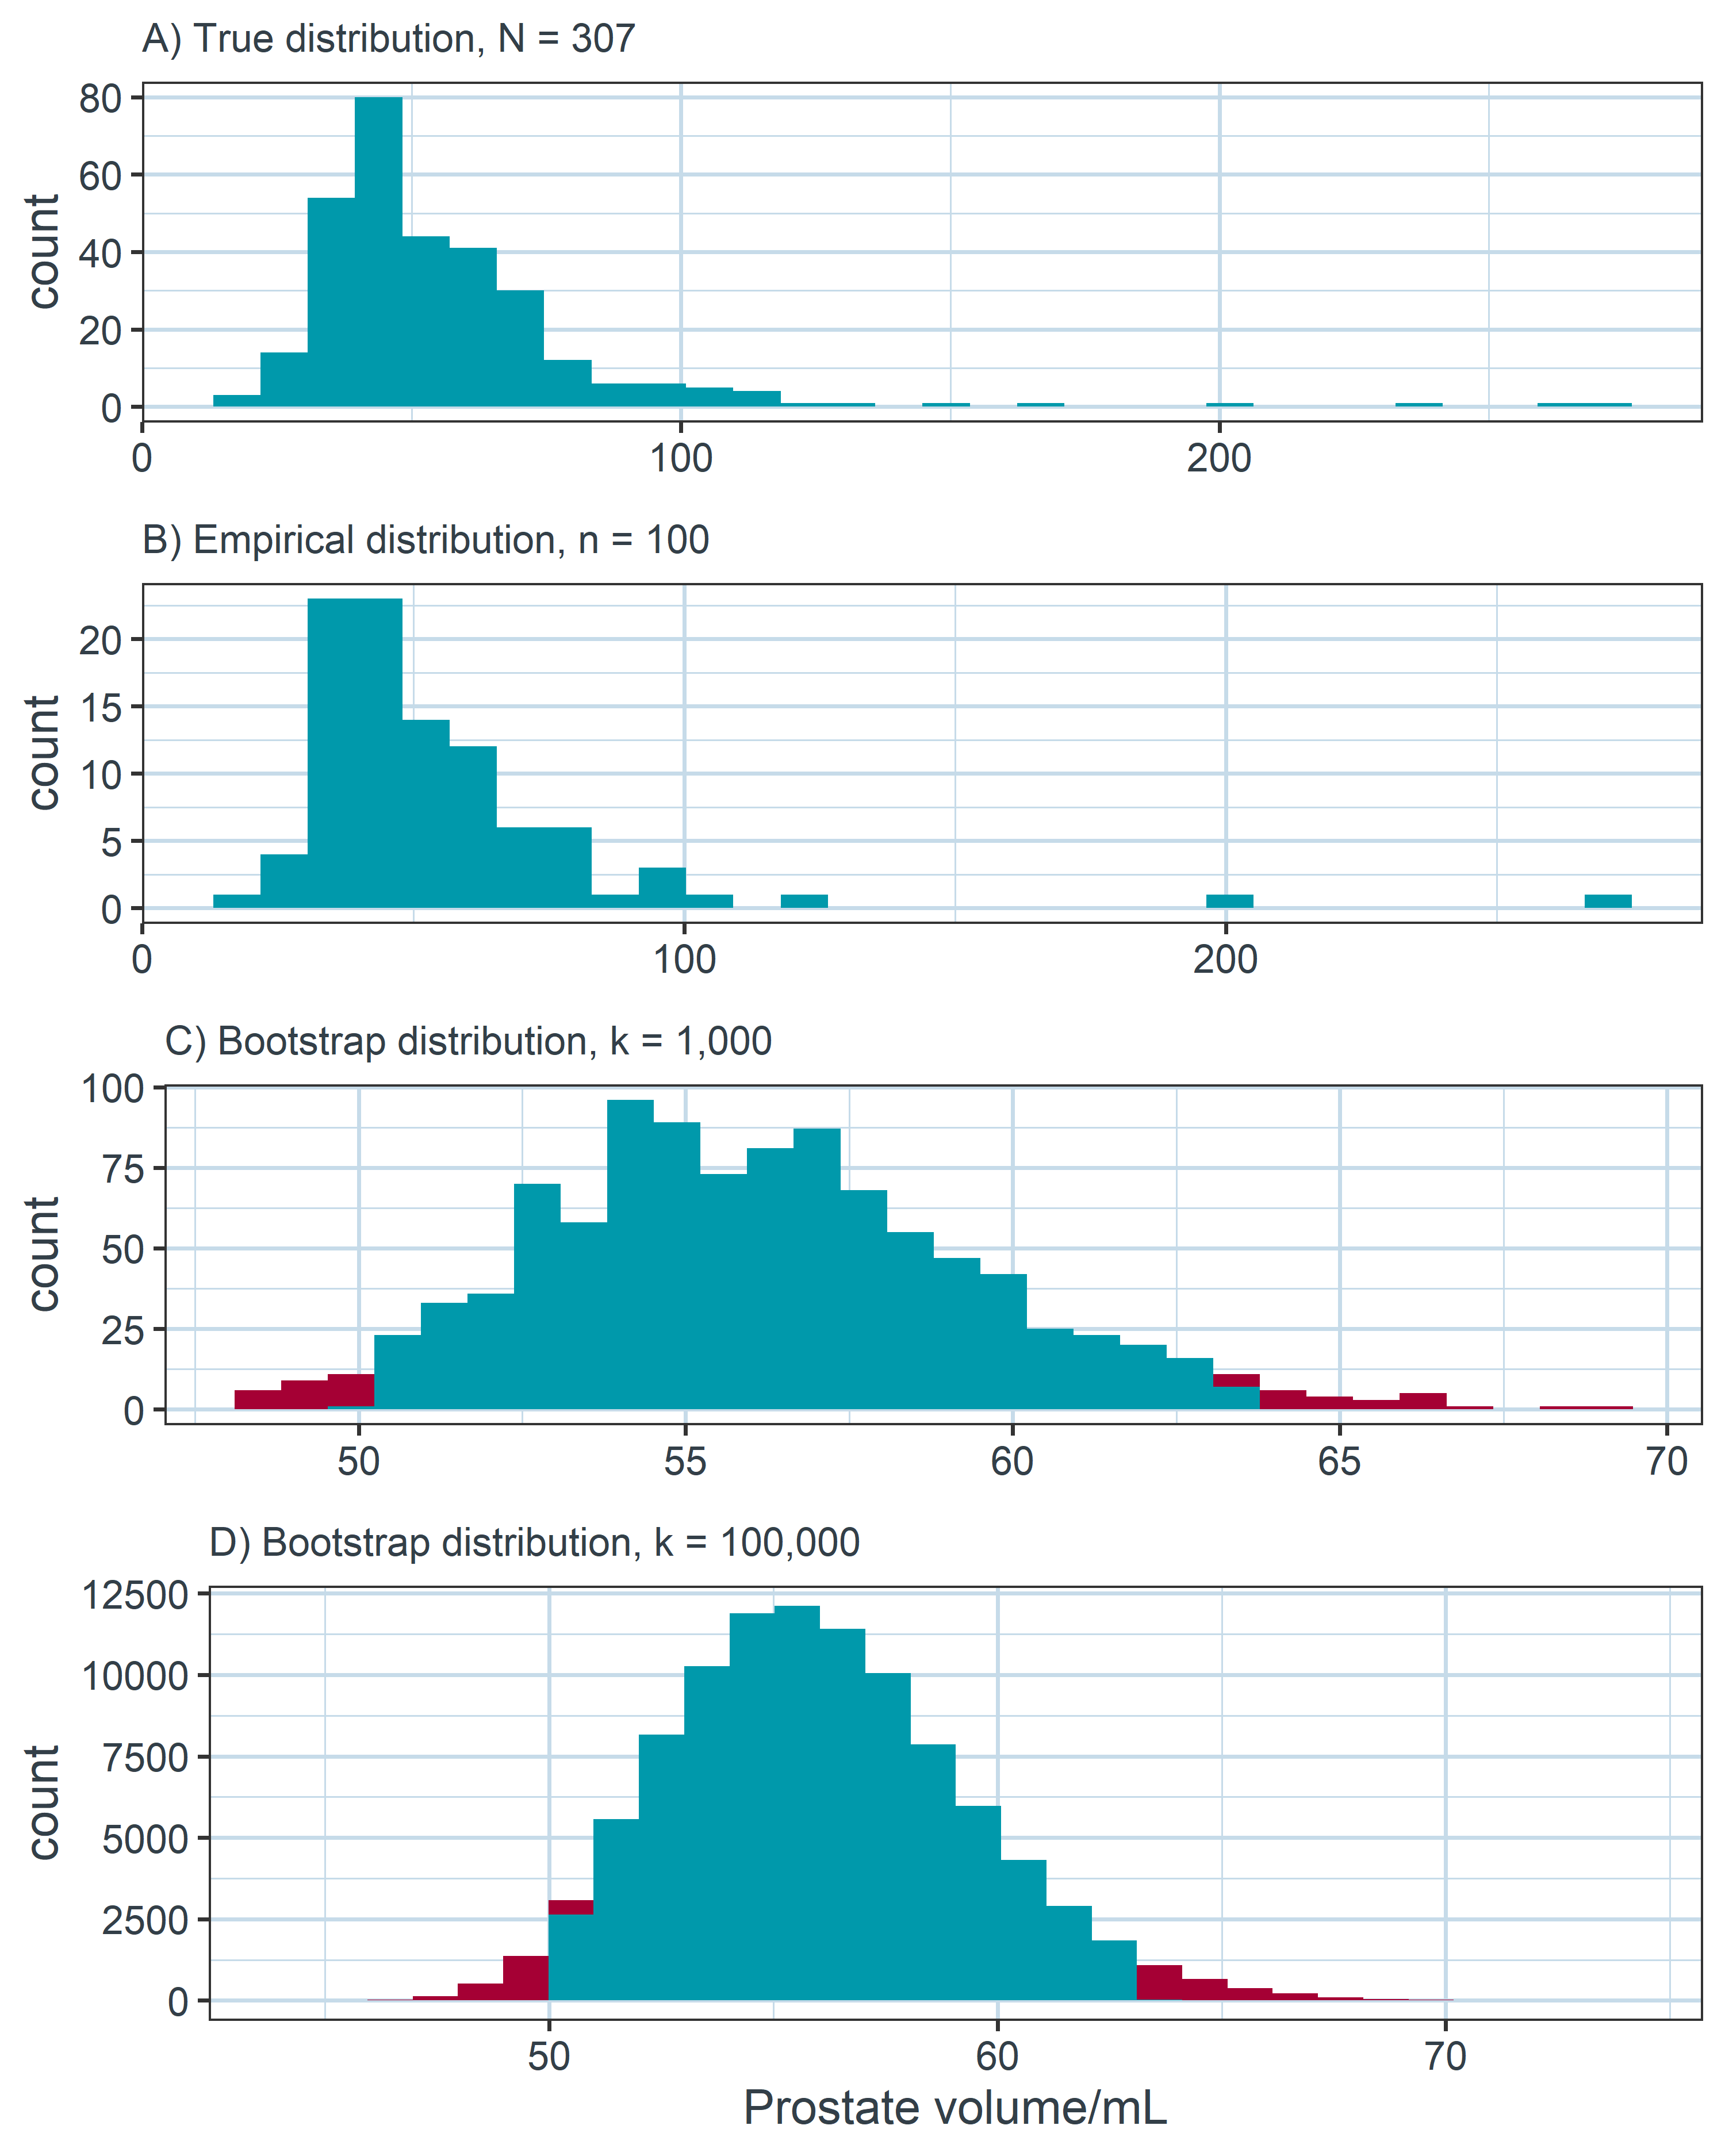
\includegraphics[keepaspectratio]{MSc_Thesis_Bookdown_files/figure-latex/prostate-vol-1.png}}
\caption{\label{fig:prostate-vol}Histograms demonstrating distribution of prostate volumes in patients with prostatic cancer, taken from Cata et al 2011\textsuperscript{\citeproc{ref-cata_blood_2011}{43}} via the R package \texttt{medicaldata}\textsuperscript{\citeproc{ref-medicaldata}{44}}. A) Distribution from whole study population of 307 patients with non-missing data, exhibiting right-skew. B) Distribution from random sample of 100 patients, still exhibiting right-skew. C) Bootstrap distribution generated by re-sampling 1,000 bootstrap samples from the original sample of 100 patients, right-skew less apparent. D) Bootstrap distribution generated by re-sampling 100,000 bootstrap samples from the original sample of 100 patients, approaching normality. 95\% confidence intervals are demonstrated in plots C and D by marking the 2.5th and 97.5th centiles.}
\end{figure}

\newpage

\subsection{Bootstrapping - Relevance to WME}\label{bootstrapping---relevance-to-wme}

In current implementations of \hyperref[acronyms_WME]{WME}, the \hyperref[acronyms_WME]{WME} estimate of the causal effect (\(\hat{\beta}_{WME}\)) is calculated as described in Bowden et al\textsuperscript{\citeproc{ref-bowden_consistent_2016}{8}}, and the 95\% \hyperref[acronyms_CI]{CI} is generated separately using bootstrapping, though notably not using the method described above.

The bootstrapping process begins similarly, with re-sampling undertaken (a default of \(k = 1000\) times) to generate \(k\) bootstrap samples \(x^{*1}, x^{*2},...x^{*k}\). Each individual bootstrap sample \(x^{*i}\) is used to estimate the causal effect using the \hyperref[acronyms_WME]{WME} method \(\hat{\beta}^{*i}_{WME}\), and thus a bootstrap distribution of \(k\) values of \hyperref[acronyms_WME]{WME} is created, \(\hat{\beta}^{*1}_{WME},  \hat{\beta}^{*2}_{WME}....\hat{\beta}^{*k}_{WME}\).

At this stage, however, the bootstrap distribution is then assumed to be approximately normally distributed without verifying this assumption. The 95\% \hyperref[acronyms_CI]{CI} of the bootstrap estimate is then calculated as 1.96 \hyperref[acronyms_SD]{SD}s of the bootstrap distribution either side of the mean estimate, i.e.~\(\hat{\beta}_{WME} \pm 1.96  \times SE\). This approach may be problematic for several reasons.

Although \hyperref[acronyms_CLT]{CLT} leads us to expect that the bootstrap distribution will approach normality as the number of bootstrap iterations \(k\) increases, the extent to which this occurs for a given \(k\) may depend on the inital distribution of values in the population \(X\), and so also on the distribution in the sample/bootstrap population \(x\). If the true distribution of values is very non-normal, as may be the case for traits determined by complex genetic and environmental influences, it may take relatively more bootstrap iterations for the bootstrap distribution to become sufficiently normal to assume mean and \hyperref[acronyms_SD]{SD} accurately describe it.

Additionally, the bootstrap \hyperref[acronyms_SE]{SE} is inversely proportional to the number of bootstrap iterations \(k\), as opposed to the usual standard error (given by \(SE = \frac{SD}{\sqrt{n}}\)), which is inversely proportional to the square root of the sample size \(n\). It is therefore possible to generate smaller \hyperref[acronyms_SE]{SE}s by increasing the number of bootstrap samples obtained. This may lead to false confidence in estimates generated despite potential issues with initial sample \(x\), e.g.~if it too small, or sampled in such a way that it is not representative of the underlying population \(X\). Although such issues are inherent to any bootstrapping approaches, the usual method of generating bootstrapped \hyperref[acronyms_CI]{CI}s detailed above uses more information (i.e.~using the entire bootstrap distribution) to generate these values than the parameter-based \(estimate \pm 1.96 \times SE\) method (i.e.~using approximate summary statistics to represent the distribution). The usual method of bootstrap \hyperref[acronyms_CI]{CI} generation may therefore be expected to highlight any variation or uncertainty present more readily than the parameter-based approach; this would be represented as wider \hyperref[acronyms_CI]{CI}s.

\newpage

\section{Appendix: Simulation Code}\label{appendix-sim}

\subsection{Generating Data and Models}\label{appendix-sim-gen}

The data generating model used was from Appendix 3 of Bowden et al\textsuperscript{\citeproc{ref-bowden_consistent_2016}{8}}; the relevant section describing their model is reproduced below:

\begin{quote}
\emph{``\ldots{}}
\end{quote}

\begin{quote}
\begin{equation} 
U_i = \sum^J_{j=1} \phi_jG_{ij} + \epsilon_i^U
\end{equation}
\end{quote}

\begin{quote}
\begin{equation} 
X_i = \sum^J_{j=1} \gamma_jG_{ij} + U_i + \epsilon_i^X
\end{equation}
\end{quote}

\begin{quote}
\begin{equation} 
Y_i = \sum^J_{j=1} \alpha_jG_{ij} + \beta X_i + U_i + \epsilon_i^Y
\end{equation}
\end{quote}

\begin{quote}
\emph{for participants indexed by \(i = 1, . . . , N\), and genetic instruments indexed by \(j = 1, . . . , J\).}
\end{quote}

\begin{quote}
\emph{The error terms \(\epsilon_i^U , \epsilon_i^X\) and \(\epsilon_i^Y\) were each drawn independently from standard normal distributions. The genetic effects on the exposure γj are drawn from a uniform distribution between 0.03 and 0.1. Pleiotropic effects \(\alpha_j\) and \(\phi_j\) were set to zero if the genetic instrument was a valid instrumental variable. Otherwise (with probability 0.1, 0.2, or 0.3):}
\end{quote}

\begin{quote}
\emph{1. In Scenario 1 (balanced pleiotropy, InSIDE satisfied), the \(\alpha_j\) parameter was drawn from a uniform distribution between −0.2 and 0.2.}
\end{quote}

\begin{quote}
\emph{2. In Scenario 2 (directional pleiotropy, InSIDE satisfied), the \(\alpha_j\) parameter was drawn from a uniform distribution between 0 and 0.2.}
\end{quote}

\begin{quote}
\emph{3. In Scenario 3 (directional pleiotropy, InSIDE not satisfied), the \(\phi_j\) parameter was drawn from a uniform distribution between −0.2 and 0.2.}
\end{quote}

\begin{quote}
\emph{The causal effect of the exposure on the outcome was either \(\beta X = 0\) (null causal effect) or \(\beta X = 0.1\) (positive causal effect). A total of 10 000 simulated datasets were generated for sample sizes of N = 10 000 and 20 {[}sic{]} participants. Only the summary data, that is genetic associations with the exposure and with the outcome and their standard errors as estimated by univariate regression on the genetic instruments in turn, were used by the analysis methods. In the two-sample setting, data were generated on 2N participants, and genetic associations with the exposure were estimated in the first N participants, and genetic associations with the outcome in the second N participants.''}\textsuperscript{\citeproc{ref-bowden_consistent_2016}{8}}
\end{quote}

To reproduce this model, code was written in R to generate the relevant participant level data. First, a function (\texttt{get\_simulated\_MR\_data}) was written which included parameters specified by Bowden et al, and also to allow testing of data simulation:

This initial simulation function generated data in the following format:

\begin{Shaded}
\begin{Highlighting}[]
\CommentTok{\# Check data produced in expected format}
\CommentTok{\#set.seed(1701)}
\NormalTok{test\_data\_sim }\OtherTok{\textless{}{-}} \FunctionTok{get\_simulated\_MR\_data}\NormalTok{(}\AttributeTok{n\_participants =} \DecValTok{1000}\NormalTok{,}
                                       \AttributeTok{n\_instruments =} \DecValTok{25}\NormalTok{,}
                                       \AttributeTok{n\_datasets =} \DecValTok{2}\NormalTok{,}
                                       \AttributeTok{prop\_invalid =} \FloatTok{0.3}\NormalTok{,}
                                       \AttributeTok{rand\_error =} \ConstantTok{FALSE}\NormalTok{,}
                                       \AttributeTok{causal\_effect =} \ConstantTok{TRUE}\NormalTok{,}
                                       \AttributeTok{balanced\_pleio =} \ConstantTok{TRUE}\NormalTok{,}
                                       \AttributeTok{InSIDE\_satisfied =} \ConstantTok{TRUE}\NormalTok{)}

\FunctionTok{str}\NormalTok{(test\_data\_sim)}
\end{Highlighting}
\end{Shaded}

\begin{verbatim}
## List of 12
##  $ U             :List of 2
##   ..$ : num [1:2000, 1] 0 0 0 0 0 0 0 0 0 0 ...
##   ..$ : num [1:2000, 1] 0 0 0 0 0 0 0 0 0 0 ...
##  $ X             :List of 2
##   ..$ : num [1:1000, 1] 1.59 1.29 1.02 1.89 1.49 ...
##   ..$ : num [1:1000, 1] 1.85 1.84 2.18 1.16 1.44 ...
##  $ Y             :List of 2
##   ..$ : num [1:1000, 1] 0.0704 0.1351 0.1589 0.0944 0.0161 ...
##   ..$ : num [1:1000, 1] 0.59017 0.10039 0.00743 0.27896 0.27746 ...
##  $ G_X           :List of 2
##   ..$ : int [1:1000, 1:25] 2 0 1 2 1 0 1 0 0 2 ...
##   ..$ : int [1:1000, 1:25] 0 1 2 1 1 1 0 2 0 2 ...
##  $ G_Y           :List of 2
##   ..$ : int [1:1000, 1:25] 1 1 0 1 2 0 1 0 1 2 ...
##   ..$ : int [1:1000, 1:25] 1 1 1 1 0 1 2 0 2 0 ...
##  $ alpha         :List of 2
##   ..$ : num [1:25] 0 0 0.1157 0 -0.0634 ...
##   ..$ : num [1:25] 0 0 0.1157 0 -0.0634 ...
##  $ gamma         :List of 2
##   ..$ : num [1:25] 0.0938 0.0808 0.0755 0.0342 0.0443 ...
##   ..$ : num [1:25] 0.0938 0.0808 0.0755 0.0342 0.0443 ...
##  $ phi           :List of 2
##   ..$ : num [1:25] 0 0 0 0 0 0 0 0 0 0 ...
##   ..$ : num [1:25] 0 0 0 0 0 0 0 0 0 0 ...
##  $ n_participants:List of 2
##   ..$ : num 1000
##   ..$ : num 1000
##  $ n_instruments :List of 2
##   ..$ : num 25
##   ..$ : num 25
##  $ prop_invalid  :List of 2
##   ..$ : num 0.3
##   ..$ : num 0.3
##  $ beta_val      :List of 2
##   ..$ : num 0.1
##   ..$ : num 0.1
\end{verbatim}

A function (\texttt{get\_models}) was then written to create linear models from each dataset generated as per Bowden et al:

These models generated estimates of the coefficient of gene-exposure association (\texttt{coeff\_G\_X}), coefficient of gene-outcome association (\texttt{coeff\_G\_Y}), and the relevant standard errors of these estimates. The values of parameters inputted were also returned to aid in further testing of data/model generation, i.e.~actual gene-exposure associations (\texttt{gamma}), pleiotropic effects of invalid instruments (\texttt{alpha}), additional pleiotropic effects when \hyperref[acronyms_InSIDE]{InSIDE} assumption not satified (\texttt{phi}), causal effect of exposure on outcome (\texttt{beta}) and the proportion of invalid genetic instruments with pleiotropic effects on the outcome (\texttt{prop\_invalid}).

\begin{Shaded}
\begin{Highlighting}[]
\NormalTok{test\_extract\_model }\OtherTok{\textless{}{-}} \FunctionTok{get\_models}\NormalTok{(test\_data\_sim)}

\FunctionTok{summary}\NormalTok{(test\_extract\_model[[}\DecValTok{1}\NormalTok{]])}
\end{Highlighting}
\end{Shaded}

\begin{verbatim}
##     dataset    Instrument   coeff_G_X        coeff_G_X_SE      
##  Min.   :1   Min.   : 1   Min.   :0.03419   Min.   :6.659e-17  
##  1st Qu.:1   1st Qu.: 7   1st Qu.:0.05645   1st Qu.:6.807e-17  
##  Median :1   Median :13   Median :0.06823   Median :6.873e-17  
##  Mean   :1   Mean   :13   Mean   :0.06791   Mean   :6.889e-17  
##  3rd Qu.:1   3rd Qu.:19   3rd Qu.:0.08594   3rd Qu.:6.935e-17  
##  Max.   :1   Max.   :25   Max.   :0.09379   Max.   :7.313e-17  
##      gamma             F_stat             R2_stat    coeff_G_Y        
##  Min.   :0.03419   Min.   :6.224e+27   Min.   :1   Min.   :-0.109067  
##  1st Qu.:0.05645   1st Qu.:6.224e+27   1st Qu.:1   1st Qu.: 0.004951  
##  Median :0.06823   Median :6.224e+27   Median :1   Median : 0.006555  
##  Mean   :0.06791   Mean   :6.224e+27   Mean   :1   Mean   : 0.013297  
##  3rd Qu.:0.08594   3rd Qu.:6.224e+27   3rd Qu.:1   3rd Qu.: 0.008890  
##  Max.   :0.09379   Max.   :6.224e+27   Max.   :1   Max.   : 0.162629  
##   coeff_G_Y_SE          alpha                phi         beta    
##  Min.   :0.001550   Min.   :-0.115363   Min.   :0   Min.   :0.1  
##  1st Qu.:0.001579   1st Qu.: 0.000000   1st Qu.:0   1st Qu.:0.1  
##  Median :0.001591   Median : 0.000000   Median :0   Median :0.1  
##  Mean   :0.001598   Mean   : 0.006717   Mean   :0   Mean   :0.1  
##  3rd Qu.:0.001624   3rd Qu.: 0.000000   3rd Qu.:0   3rd Qu.:0.1  
##  Max.   :0.001653   Max.   : 0.156224   Max.   :0   Max.   :0.1  
##   prop_invalid n_instruments n_participants
##  Min.   :0.3   Min.   :25    Min.   :1000  
##  1st Qu.:0.3   1st Qu.:25    1st Qu.:1000  
##  Median :0.3   Median :25    Median :1000  
##  Mean   :0.3   Mean   :25    Mean   :1000  
##  3rd Qu.:0.3   3rd Qu.:25    3rd Qu.:1000  
##  Max.   :0.3   Max.   :25    Max.   :1000
\end{verbatim}

\newpage

\subsection{Testing Generation of Data and Models}\label{appendix-sim-test}

A series of test plots were used to verify that data were simulated as intended under the various conditions specified by input parameters. Test plots were not created for the parameters \texttt{n\_participants}, \texttt{n\_instruments} or \texttt{n\_datasets}, as the functioning of these parameters could be readily inferred from the structure of the datasets outputted, as above.

\subsubsection{Proportion of Invalid Instruments}\label{proportion-of-invalid-instruments}

\leavevmode\newline The \texttt{prop\_invalid} parameter specifies the proportion of invalid genetic instruments simulated, i.e.~the proportion of genetic instruments affecting the outcome via direct/pleiotropic effects, and thus not solely via the exposure of interest. If simulated correctly, increasing the value of \texttt{prop\_invalid} should increase the number of instruments with pleiotropic effects, i.e.~instruments with \texttt{alpha} \(\ne\) 0. With random error terms set to 0 and no causal effect present (i.e.~\texttt{rand\_error\ =\ FALSE} and \texttt{causal\_effect\ =\ FALSE}), the estimated gene-outcome coefficient estimated using any given instrument will equal the pleiotropic effects of that instrument (i.e.~\texttt{coeff\_G\_Y\ =\ alpha}), and therefore will only be non-zero for invalid instruments with non-zero pleiotropic effects on the outcome . Plotting \texttt{coeff\_G\_Y} against \texttt{alpha} for simulated data with no causal effect or random error should therefore yield a graph where

\begin{itemize}
\tightlist
\item
  For valid instruments: gene-outcome coefficient = alpha = 0
\item
  For invalid instruments: gene-outcome coefficient = alpha \(\ne\) 0, with values spread uniformly between \texttt{alpha\_min} and \texttt{alpha\_max}
\end{itemize}

\pandocbounded{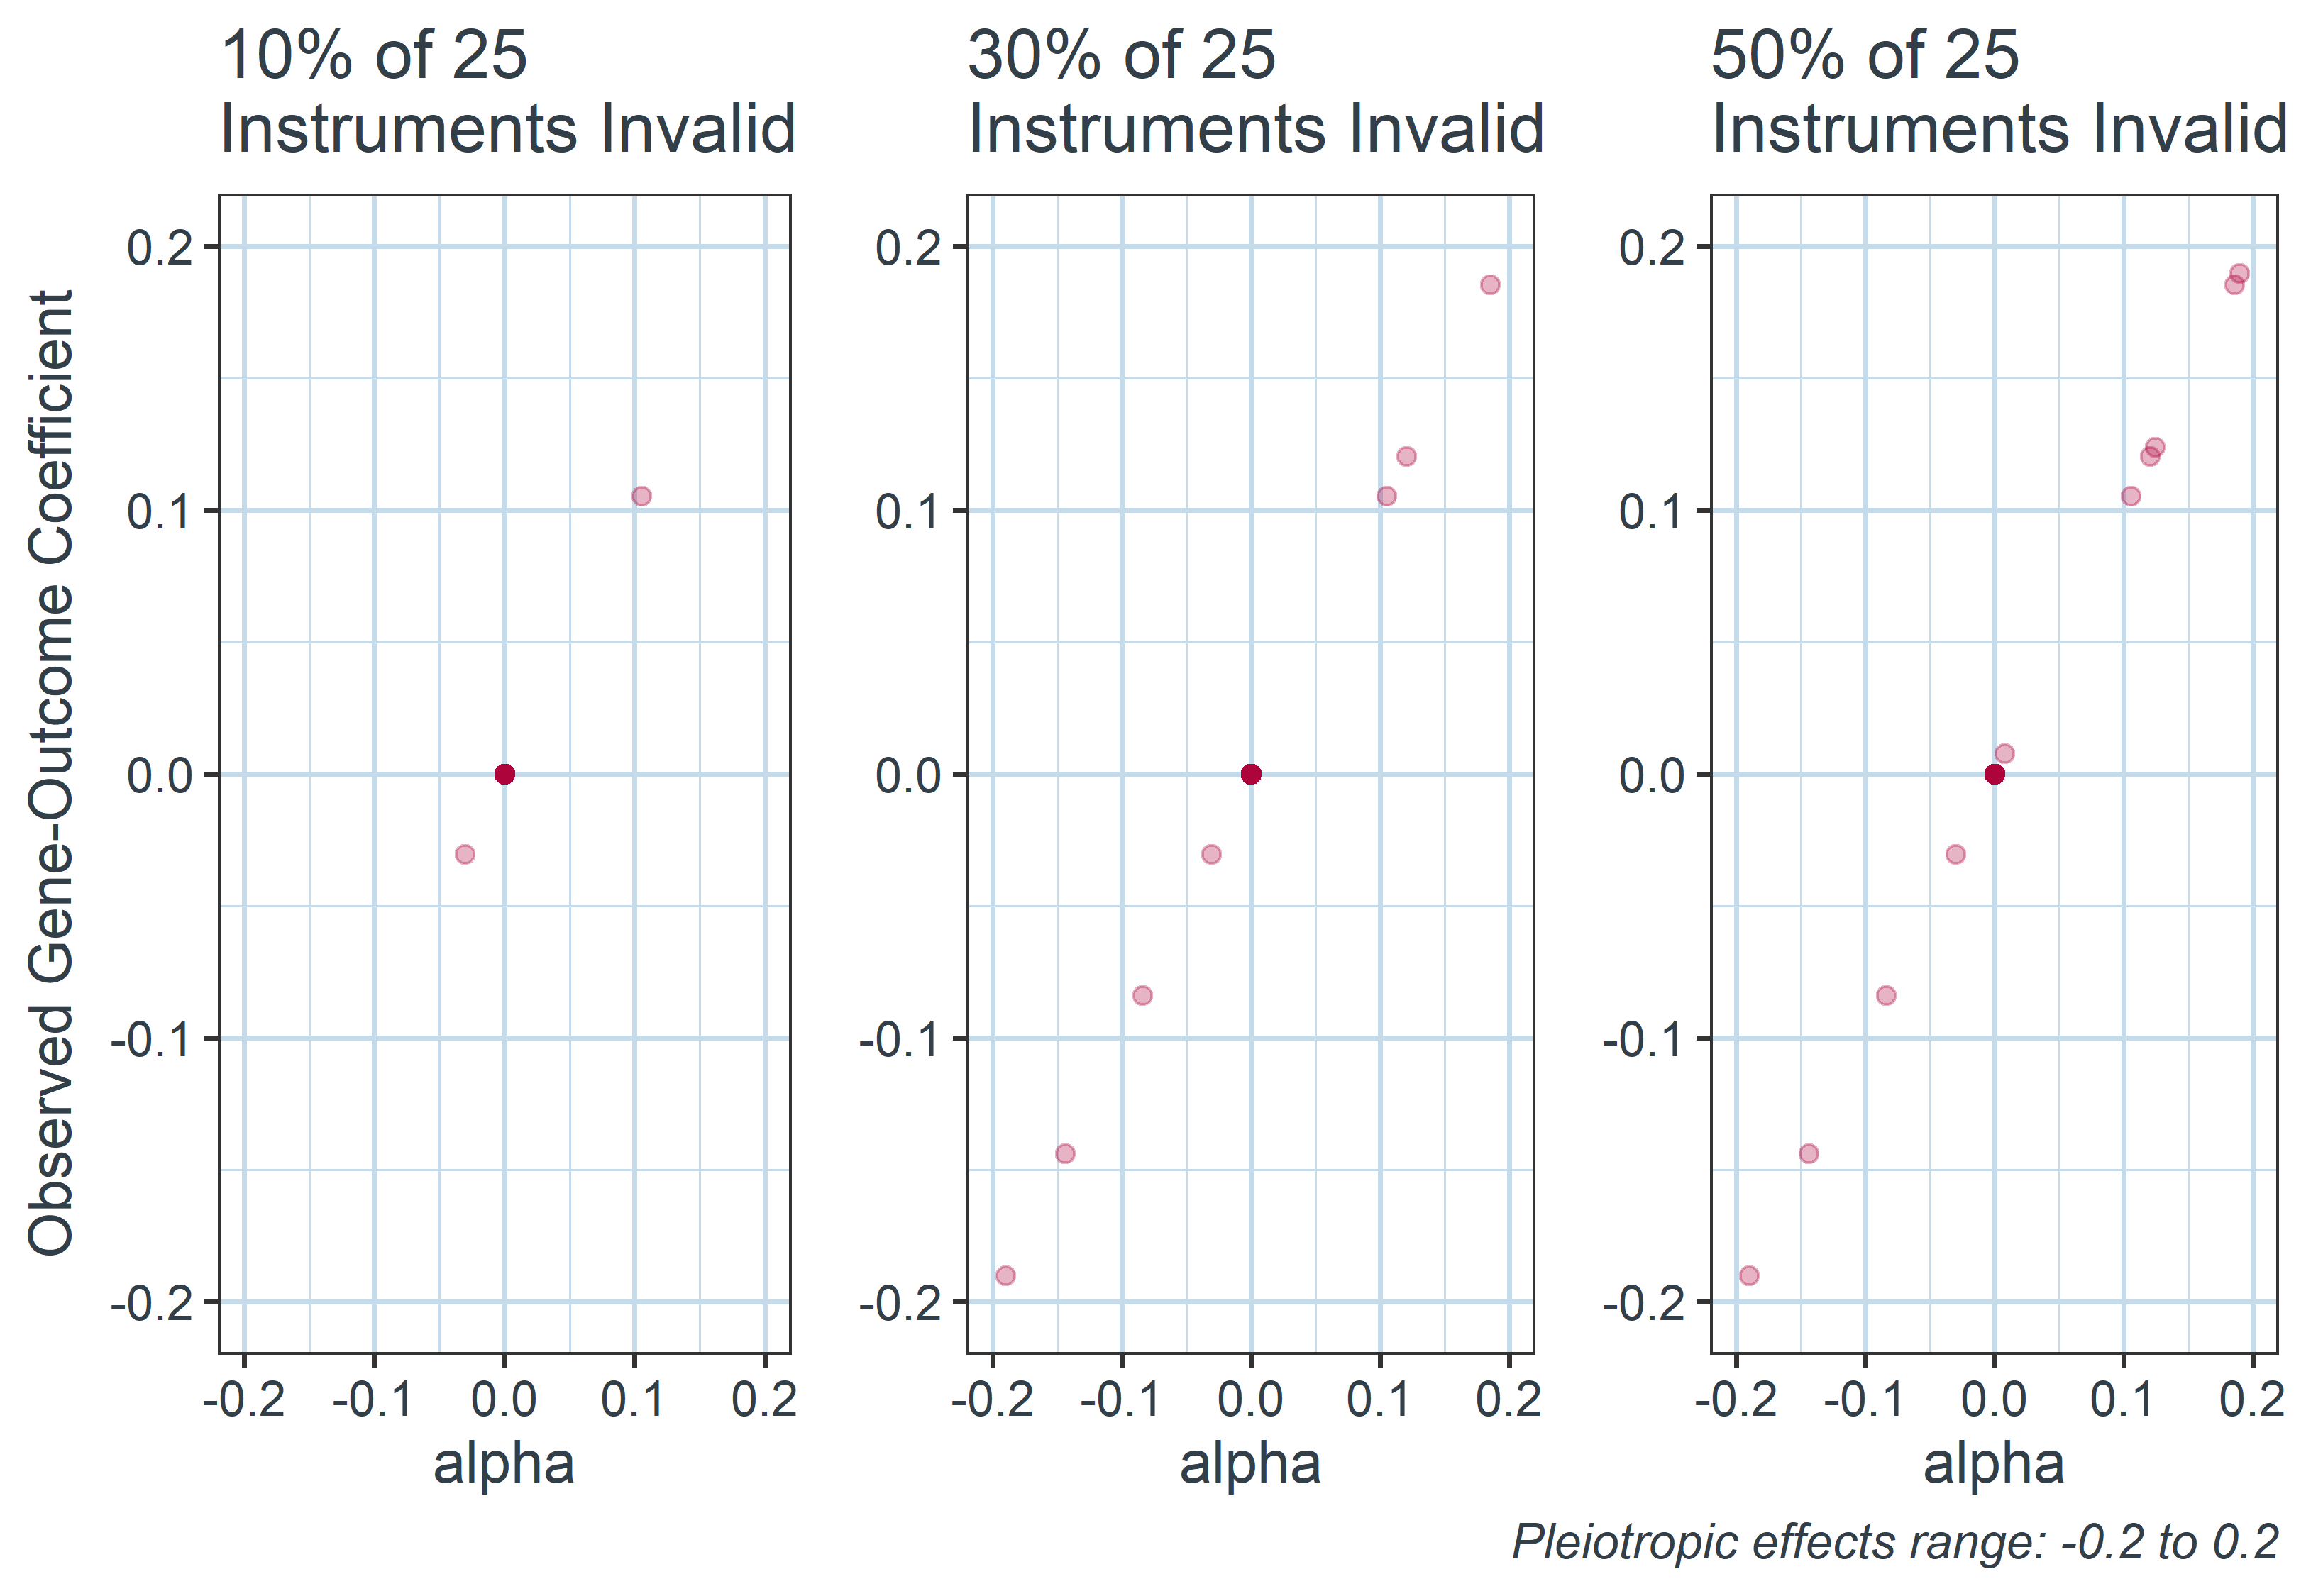
\includegraphics[keepaspectratio]{MSc_Thesis_Bookdown_files/figure-latex/test-plot-prop-invalid-1.png}}

\newpage

Similarly, with random error terms set to 0 (\texttt{rand\_error\ =\ FALSE}) and no causal effect present (\texttt{causal\_effect\ =\ FALSE}), gene-exposure coefficients estimated for each instrument should exactly match the actual values simulated, i.e.~\texttt{coeff\_G\_X\ =\ gamma} for all instruments:

\pandocbounded{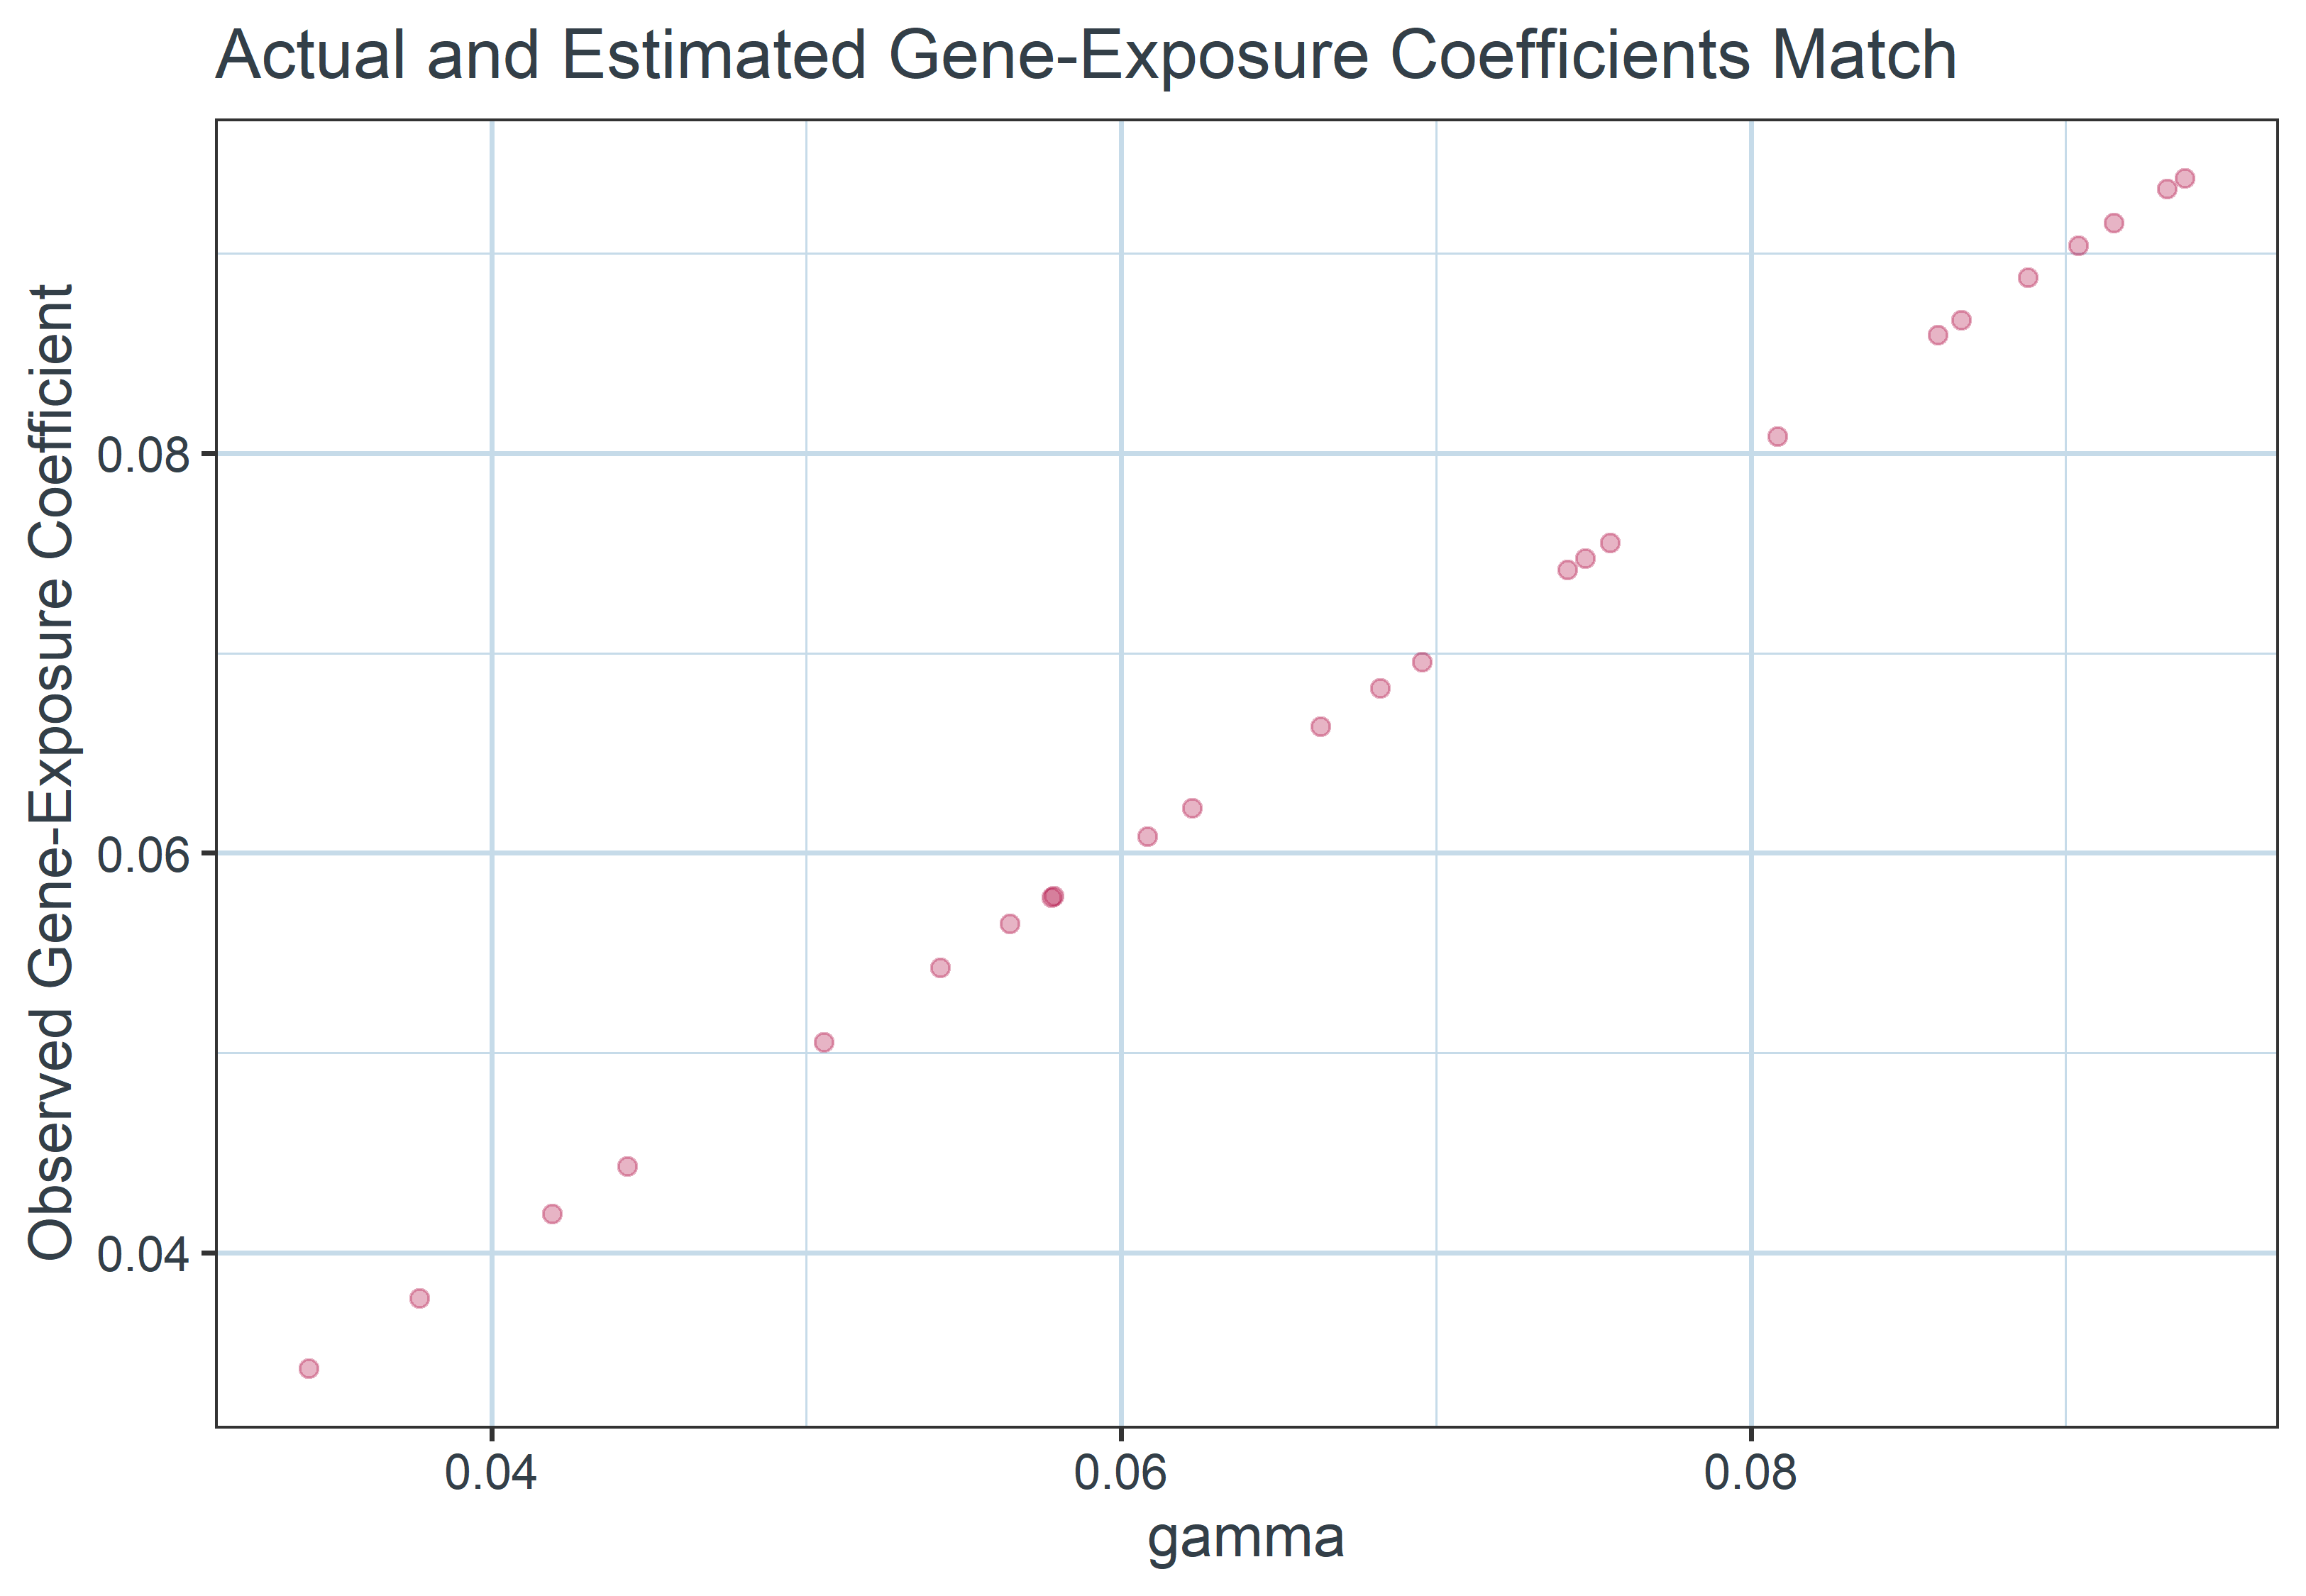
\includegraphics[keepaspectratio]{MSc_Thesis_Bookdown_files/figure-latex/test-plot-gamma-1-1.png}}

\newpage

\subsubsection{Gene-Exposure Coefficient Versus Gene-Outcome Coefficient Plots}\label{gene-exposure-coefficient-versus-gene-outcome-coefficient-plots}

\leavevmode\newline For the next phase of testing, a function (\texttt{plot\_GY\_GX}) was written to plot the coefficients for gene-exposure versus gene-outcome as estimated using the previously created linear models:

\begin{Shaded}
\begin{Highlighting}[]
\NormalTok{plot\_GY\_GX }\OtherTok{\textless{}{-}} \ControlFlowTok{function}\NormalTok{(model\_tib, }
                       \AttributeTok{plot\_title =} \FunctionTok{as.character}\NormalTok{(}\ConstantTok{NA}\NormalTok{),}
                       \AttributeTok{x\_min =} \DecValTok{0}\NormalTok{,                     }\CommentTok{\# set x{-}axis limits}
                       \AttributeTok{x\_max =} \FloatTok{0.1}\NormalTok{,}
                       \AttributeTok{y\_min =} \SpecialCharTok{{-}}\FloatTok{0.05}\NormalTok{,                 }\CommentTok{\# set x{-}axis limits}
                       \AttributeTok{y\_max =} \FloatTok{0.06}\NormalTok{,}
                       \AttributeTok{beta\_x =} \FloatTok{0.075}\NormalTok{,                }\CommentTok{\# set beta{-}hat position}
                       \AttributeTok{beta\_y =} \FloatTok{0.05}\NormalTok{,}
                       \AttributeTok{hat\_offset =} \FloatTok{0.003}
\NormalTok{)}
\NormalTok{\{}
  
\NormalTok{  model\_tib }\SpecialCharTok{\%\textgreater{}\%} 
    \FunctionTok{mutate}\NormalTok{(}\AttributeTok{Gradient =} \FunctionTok{round}\NormalTok{(}\FunctionTok{coefficients}\NormalTok{(}\FunctionTok{lm}\NormalTok{(coeff\_G\_Y }\SpecialCharTok{\textasciitilde{}} \DecValTok{0} \SpecialCharTok{+}\NormalTok{ coeff\_G\_X)[}\DecValTok{1}\NormalTok{], }\DecValTok{5}\NormalTok{), }
                            \AttributeTok{digits =} \DecValTok{2}\NormalTok{)) }\SpecialCharTok{\%\textgreater{}\%}
    \FunctionTok{plot\_template}\NormalTok{() }\SpecialCharTok{+} \CommentTok{\# pre{-}formatted plot template {-} call to ggplot with UoE colours}
    \FunctionTok{aes}\NormalTok{(}\AttributeTok{x =}\NormalTok{ coeff\_G\_X, }\AttributeTok{y =}\NormalTok{ coeff\_G\_Y) }\SpecialCharTok{+}
    \FunctionTok{geom\_point}\NormalTok{(}\AttributeTok{colour =}\NormalTok{ edin\_bright\_red\_hex, }\AttributeTok{alpha =} \FloatTok{0.3}\NormalTok{) }\SpecialCharTok{+}
    \FunctionTok{geom\_abline}\NormalTok{(}\FunctionTok{aes}\NormalTok{(}\AttributeTok{intercept =} \DecValTok{0}\NormalTok{, }
                    \AttributeTok{slope =}\NormalTok{ Gradient),}
                \AttributeTok{size =} \DecValTok{1}\NormalTok{,}
                \AttributeTok{colour =}\NormalTok{ edin\_uni\_blue\_hex) }\SpecialCharTok{+}
    \FunctionTok{geom\_text}\NormalTok{(}\FunctionTok{aes}\NormalTok{(}\AttributeTok{label =} \FunctionTok{paste0}\NormalTok{(}\StringTok{"\textbackslash{}U03B2 = "}\NormalTok{, }\FunctionTok{as.character}\NormalTok{(Gradient))), }\CommentTok{\#beta}
              \AttributeTok{x =}\NormalTok{ beta\_x, }\CommentTok{\# labels with gradient (causal effect estimate)}
              \AttributeTok{y =}\NormalTok{ beta\_y,}
              \AttributeTok{colour =}\NormalTok{ edin\_uni\_blue\_hex, }
              \AttributeTok{hjust =} \DecValTok{0}\NormalTok{, }
              \AttributeTok{data =}\NormalTok{ . }\SpecialCharTok{\%\textgreater{}\%} \FunctionTok{slice\_head}\NormalTok{()}\CommentTok{\# prevent over{-}printing}
\NormalTok{    ) }\SpecialCharTok{+}
    \CommentTok{\#label = expression("True" \textasciitilde{} hat(beta)\textasciitilde{} "= 0.25"),}
    \FunctionTok{annotate}\NormalTok{(}\StringTok{"text"}\NormalTok{,}
             \AttributeTok{x =}\NormalTok{ beta\_x,      }\CommentTok{\# add hat to beta}
             \AttributeTok{y =}\NormalTok{ beta\_y }\SpecialCharTok{+}\NormalTok{ hat\_offset,}
             \AttributeTok{label =} \FunctionTok{paste}\NormalTok{(}\StringTok{"\textbackslash{}U02C6"}\NormalTok{),}
             \AttributeTok{colour =}\NormalTok{ edin\_uni\_blue\_hex, }
             \AttributeTok{hjust =} \SpecialCharTok{{-}}\FloatTok{0.4}\NormalTok{,}
             \AttributeTok{vjust =} \FloatTok{0.9}
\NormalTok{    ) }\SpecialCharTok{+}
    \FunctionTok{labs}\NormalTok{(}\AttributeTok{title =}\NormalTok{ plot\_title,}
         \AttributeTok{x =} \StringTok{"Gene{-}Exposure Coefficient"}\NormalTok{,}
         \AttributeTok{y =} \StringTok{"Gene{-}Outcome Coefficient"}\NormalTok{) }\SpecialCharTok{+}
    \FunctionTok{xlim}\NormalTok{(x\_min, x\_max) }\SpecialCharTok{+}
    \FunctionTok{ylim}\NormalTok{(y\_min, y\_max)}
  
\NormalTok{\}}
\end{Highlighting}
\end{Shaded}

\newpage

With random error terms set to 0 (\texttt{rand\_error\ =\ FALSE}) and no causal effect present, a graph of gene-exposure coefficients versus gene-outcome coefficients should be a straight line through the origin with gradient = 0; causal effect of \(\beta\) = 0.1 present (\texttt{beta\_val\ =\ 0.1}, \texttt{causal\_effect\ =\ TRUE}), the slope of a graph of gene-exposure coefficients versus gene-outcome coefficients from the same sample should be a straight line through the origin with gradient = 0.1:

\pandocbounded{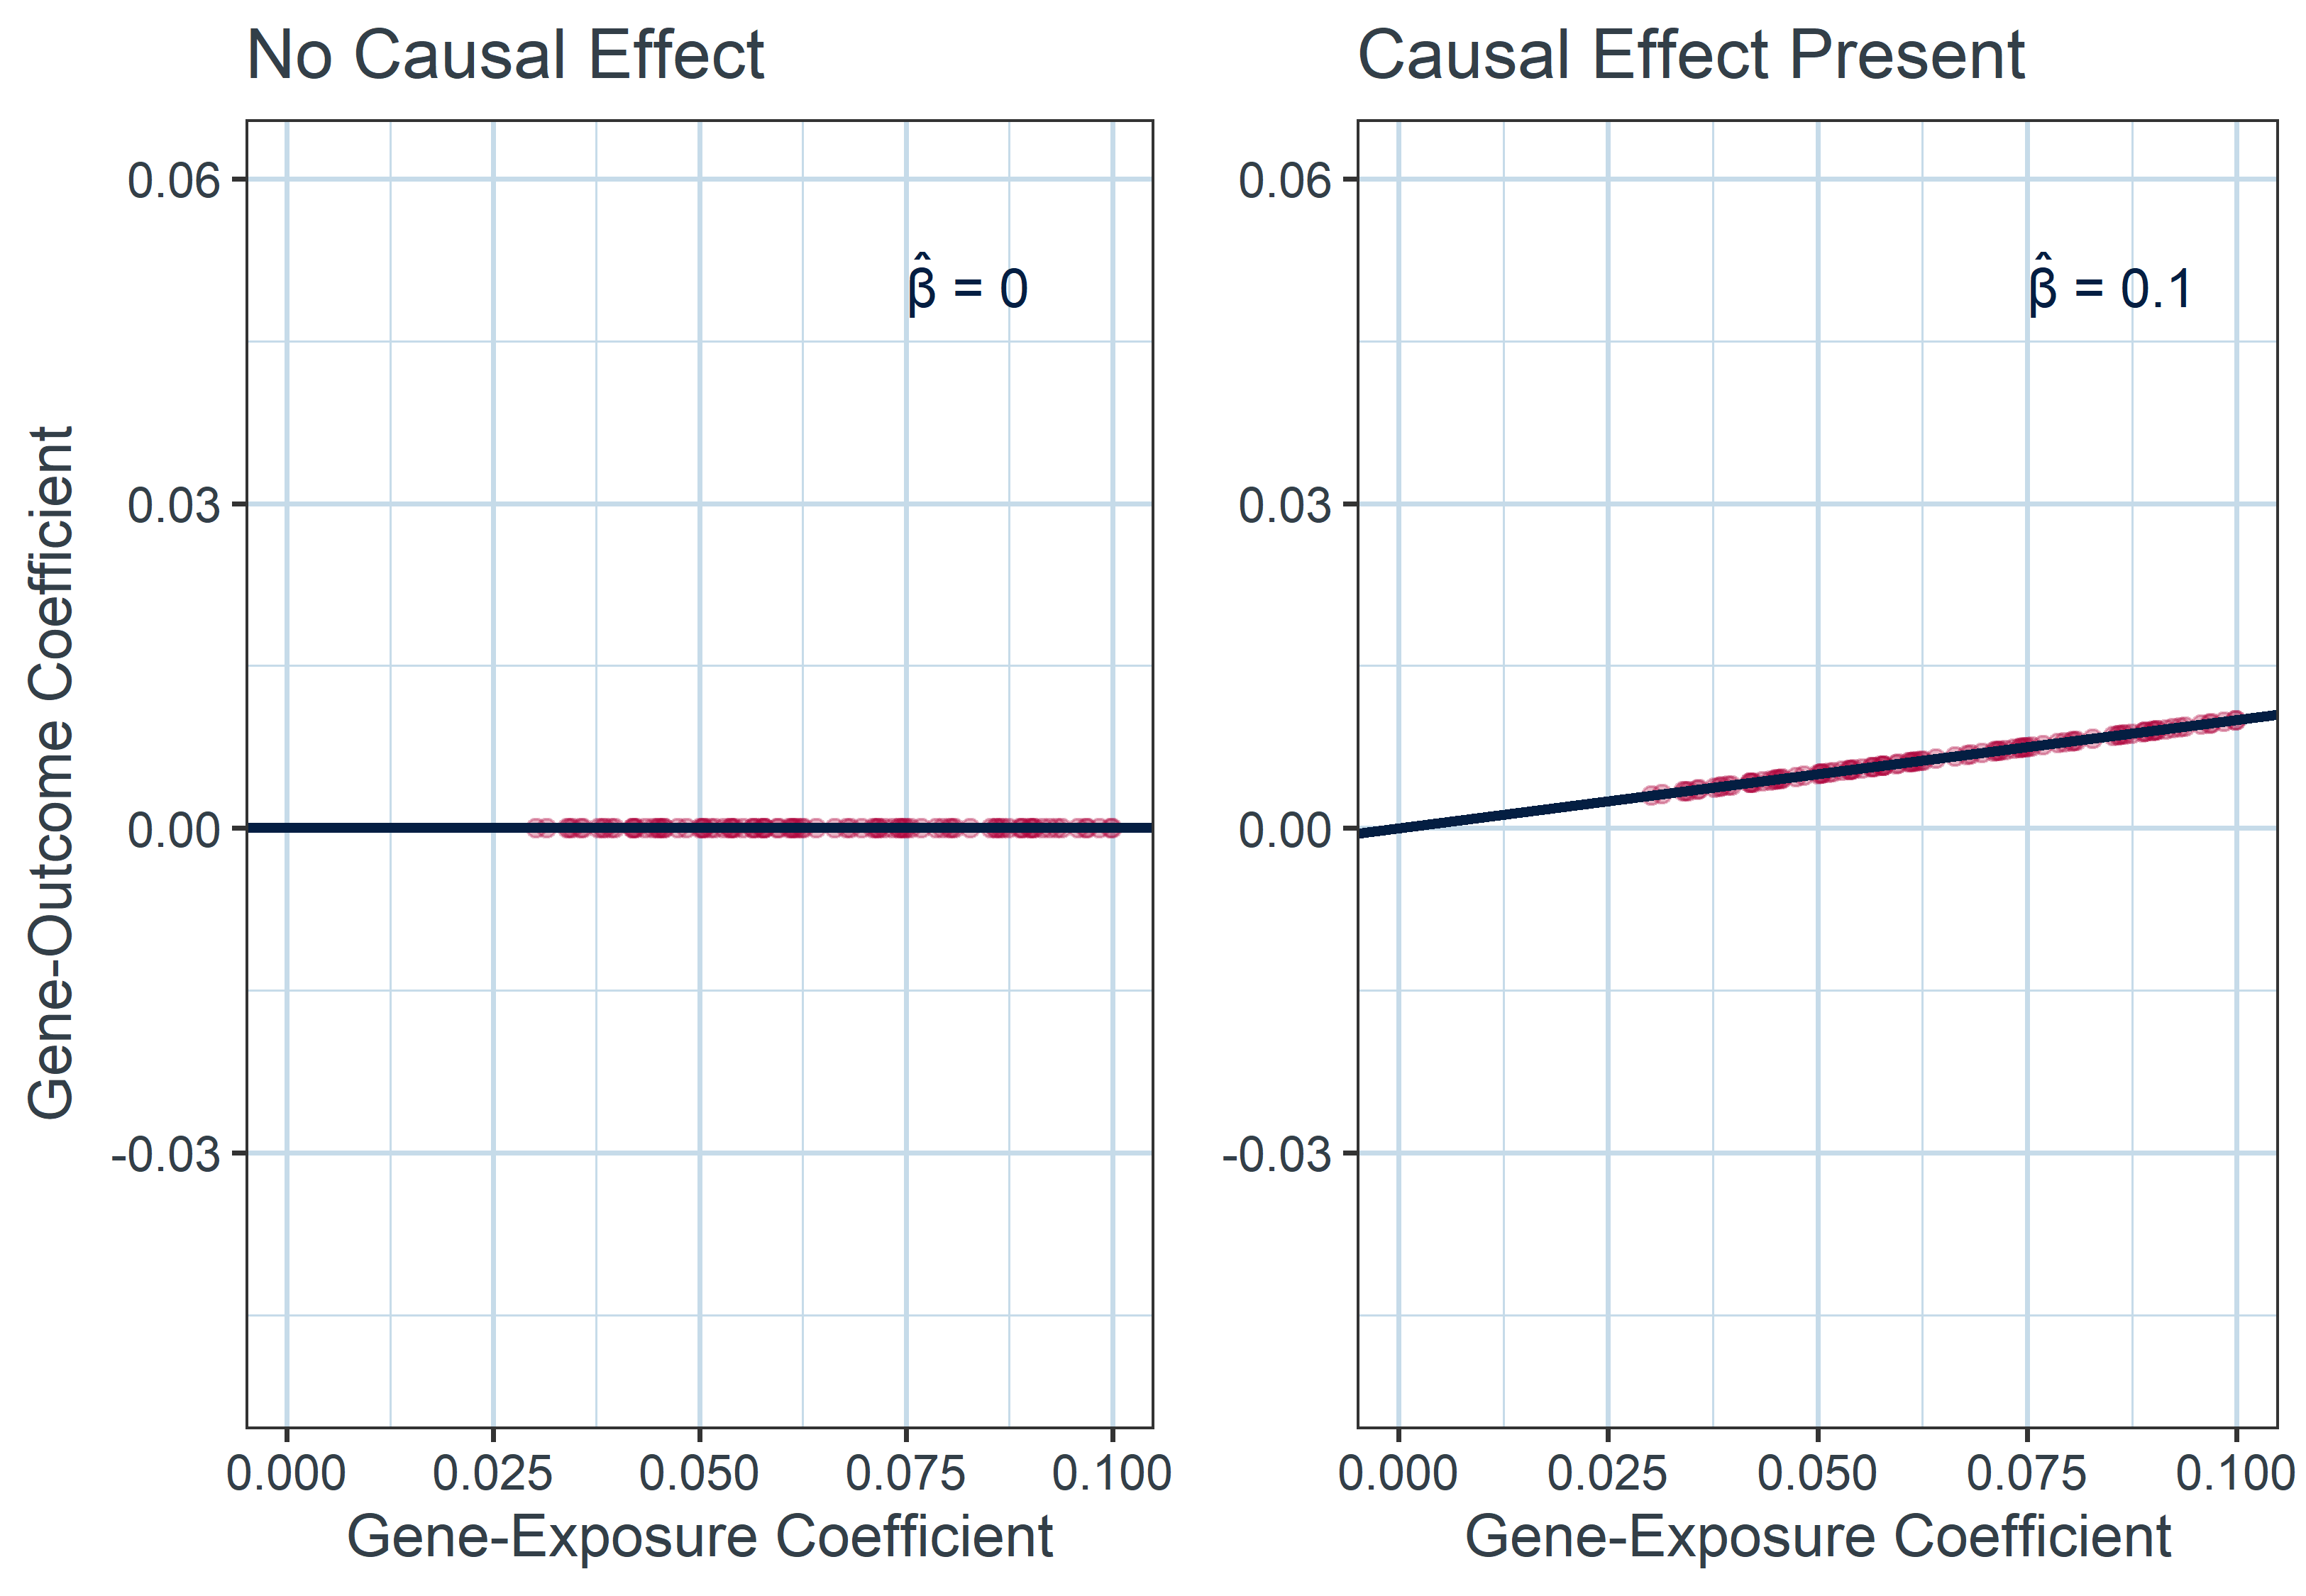
\includegraphics[keepaspectratio]{MSc_Thesis_Bookdown_files/figure-latex/test-plot-causal-1.png}}

\newpage

\subsubsection{Random Errors}\label{random-errors}

\leavevmode\newline Re-plotting the same graphs with non-zero random error terms (\texttt{rand\_error\ =\ TRUE}) should produce similar graphs with Gaussian spread around lines passing through the origin with gradients of 0 and 0.1 for no causal effect and causal effect, respectively:

\pandocbounded{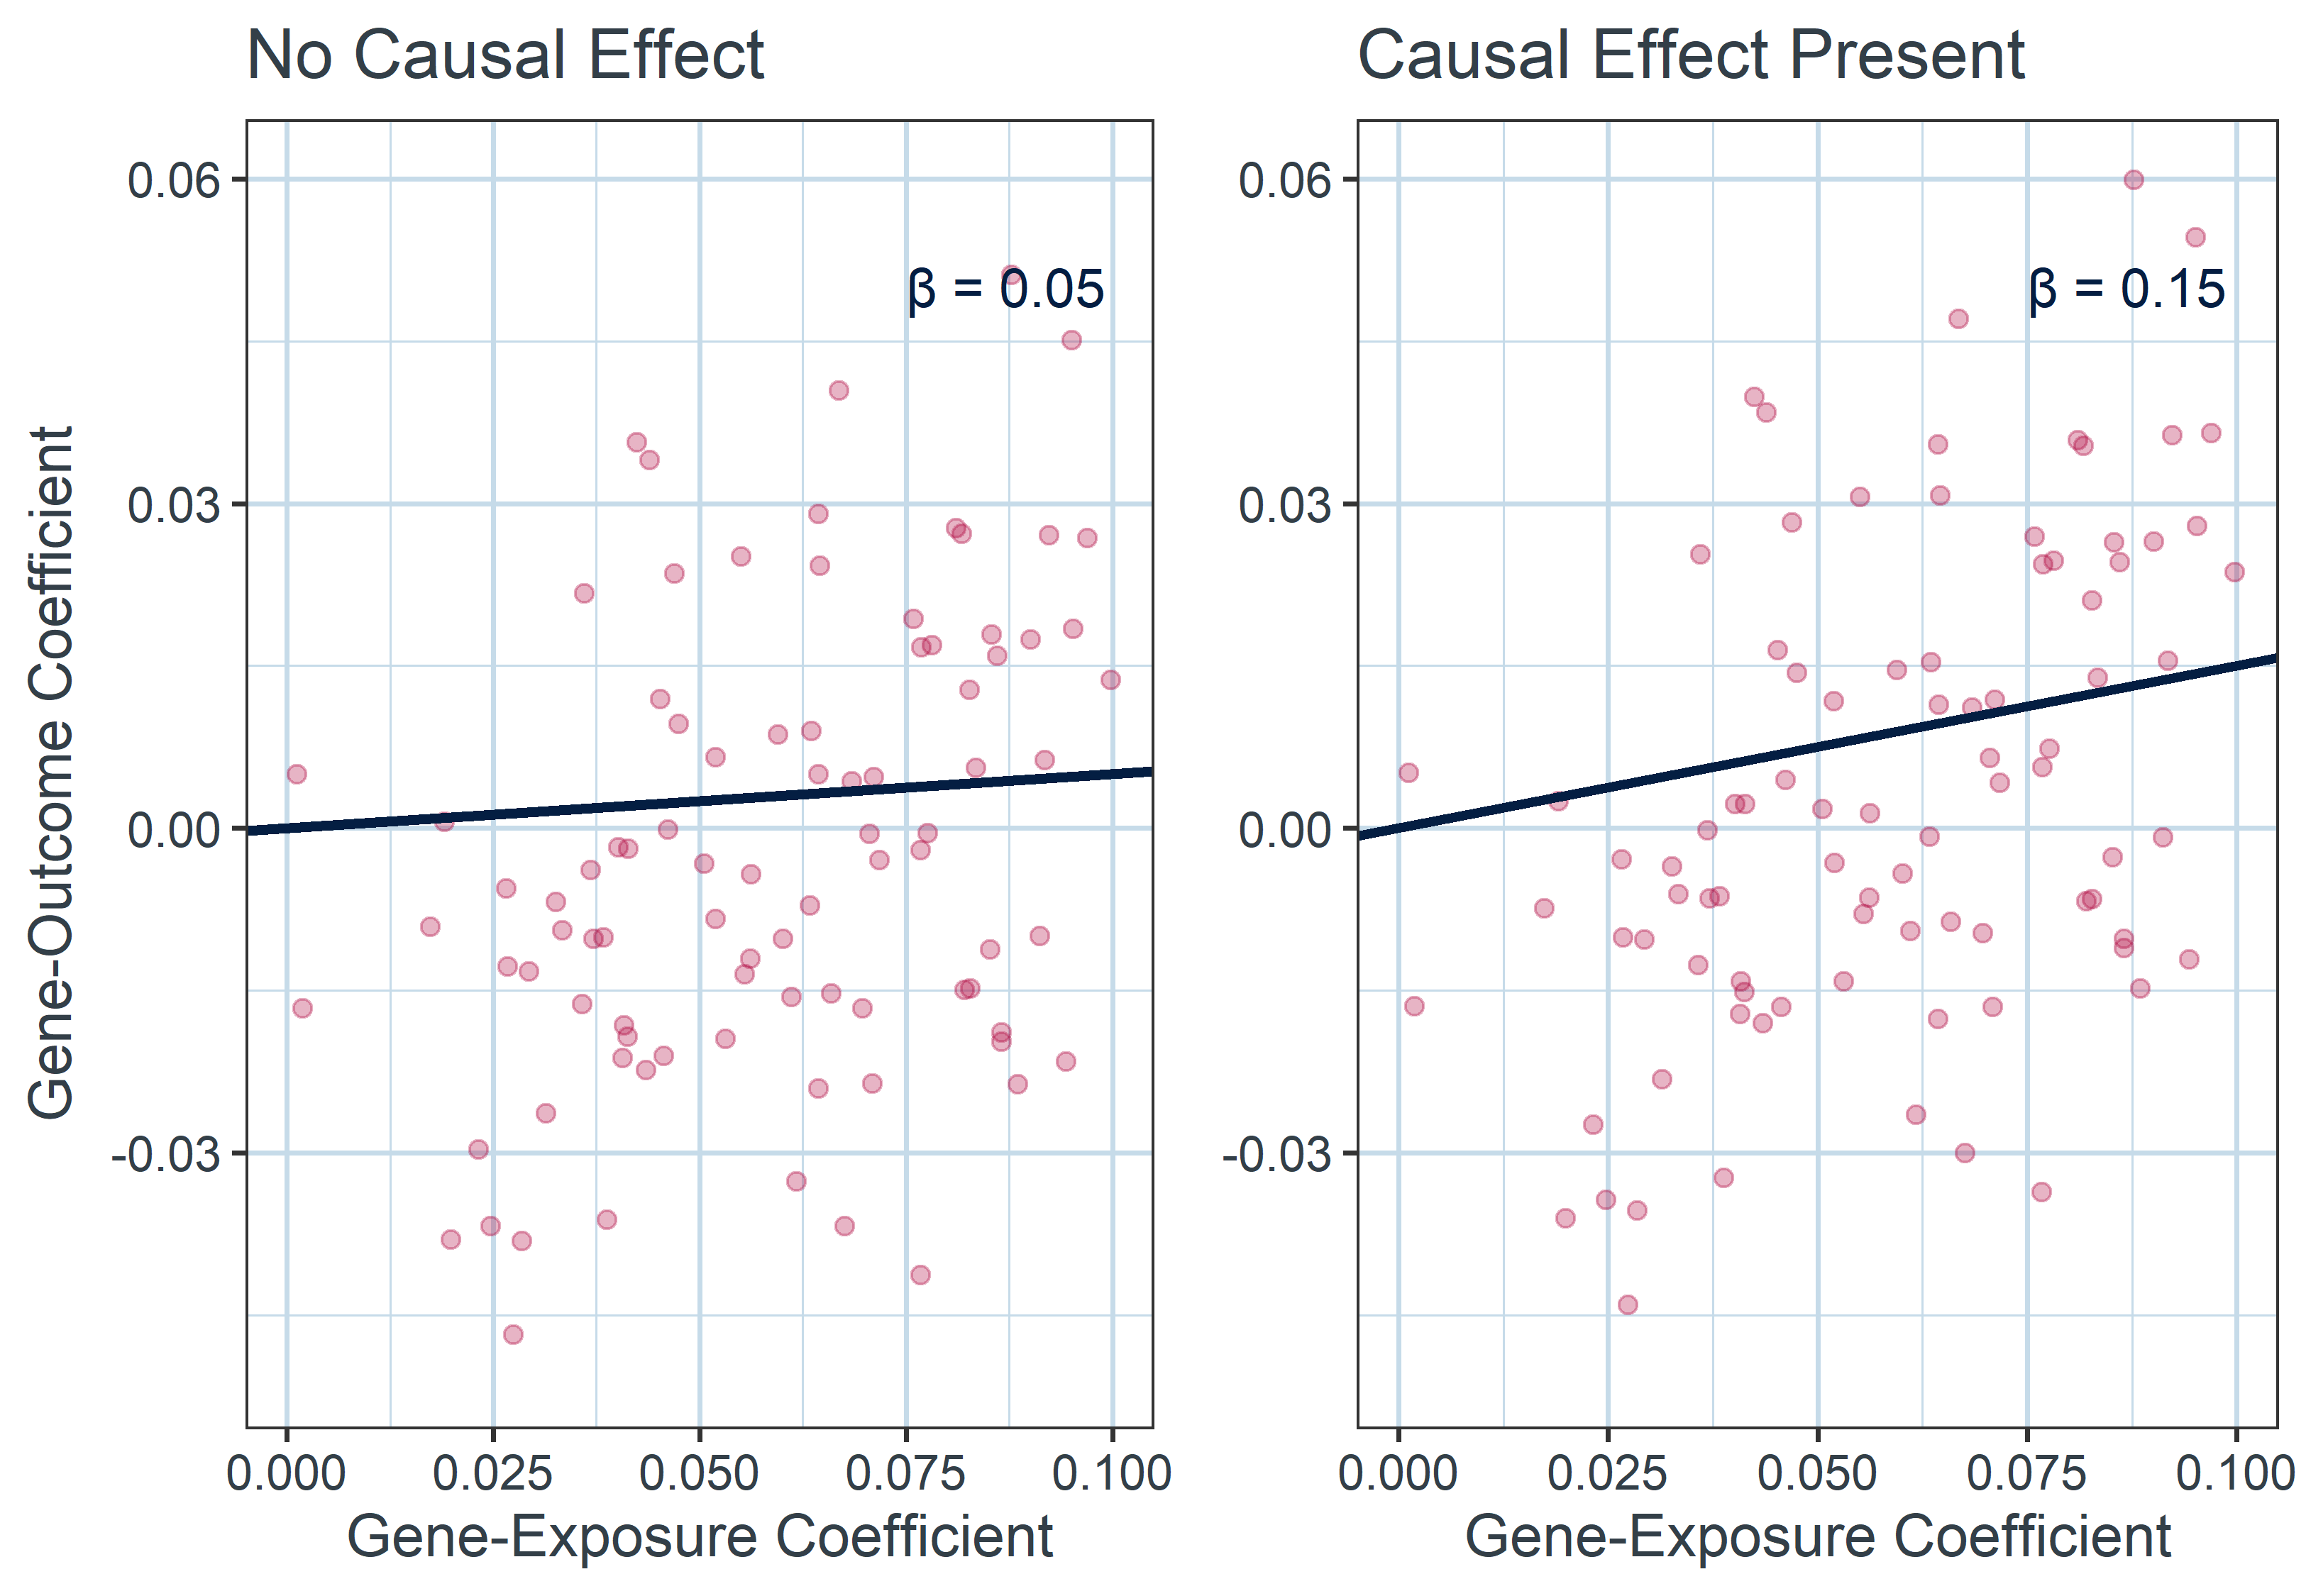
\includegraphics[keepaspectratio]{MSc_Thesis_Bookdown_files/figure-latex/test-plot-causal-errors-1.png}}

\newpage

\subsubsection{One versus Two Sample MR}\label{one-versus-two-sample-mr}

\leavevmode\newline Where gene-exposure coefficients and gene-outcome coefficients are estimated from two separate samples rather than one (i.e.~\texttt{two\_sample\ =\ TRUE}, simulating 2 sample MR), even with random error terms set to zero, error will be introduced into causal effect estimation through random sampling of different combinations of effect alleles. However, where a causal effect is not present, the effect estimated will consistently be zero regardless of the combinations of alleles sampled, so random error should not be introduced:

\pandocbounded{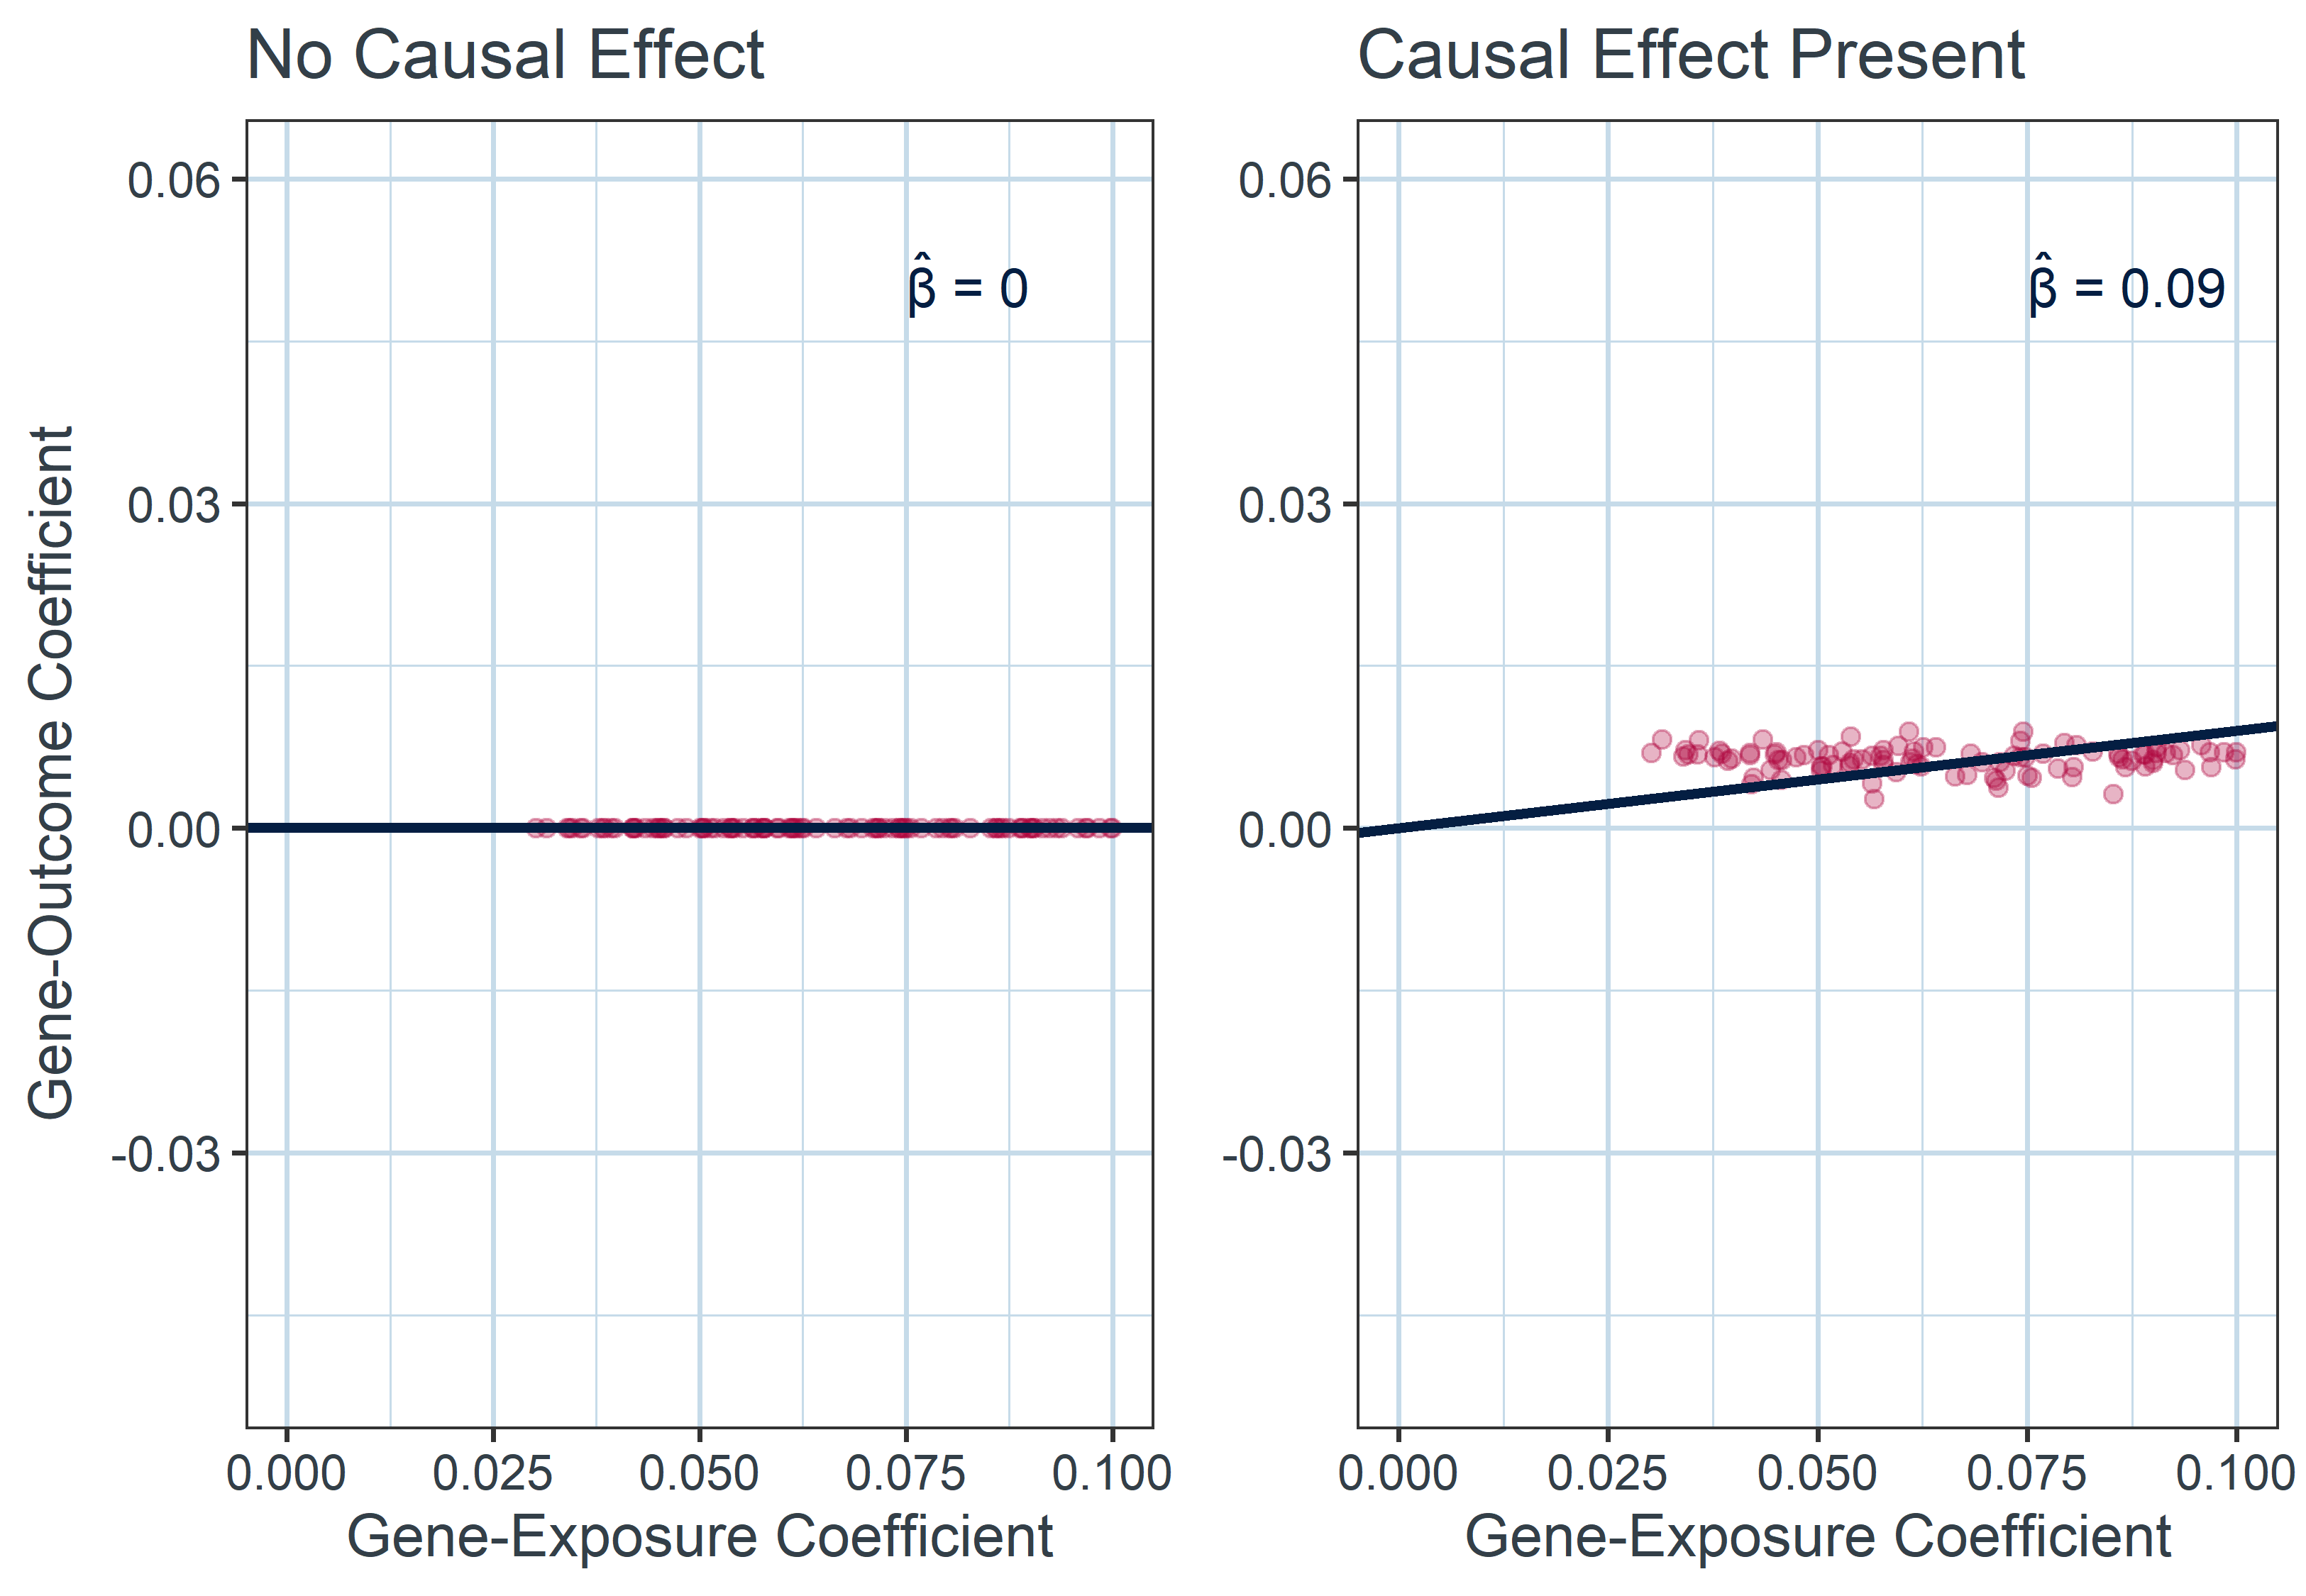
\includegraphics[keepaspectratio]{MSc_Thesis_Bookdown_files/figure-latex/test-plot-causal-2SMR-1.png}}

\newpage

\subsubsection{Invalid Instruments}\label{invalid-instruments}

\leavevmode\newline Where invalid instruments are present (i.e.~\texttt{prop\_invalid} \(\ne\) \texttt{0}) and random error terms are set to 0, graphs of gene-exposure coefficients versus gene-outcome coefficients should be straight lines through the origin and all points representing valid instruments; the invalid instruments should appear as outliers to this line:

\pandocbounded{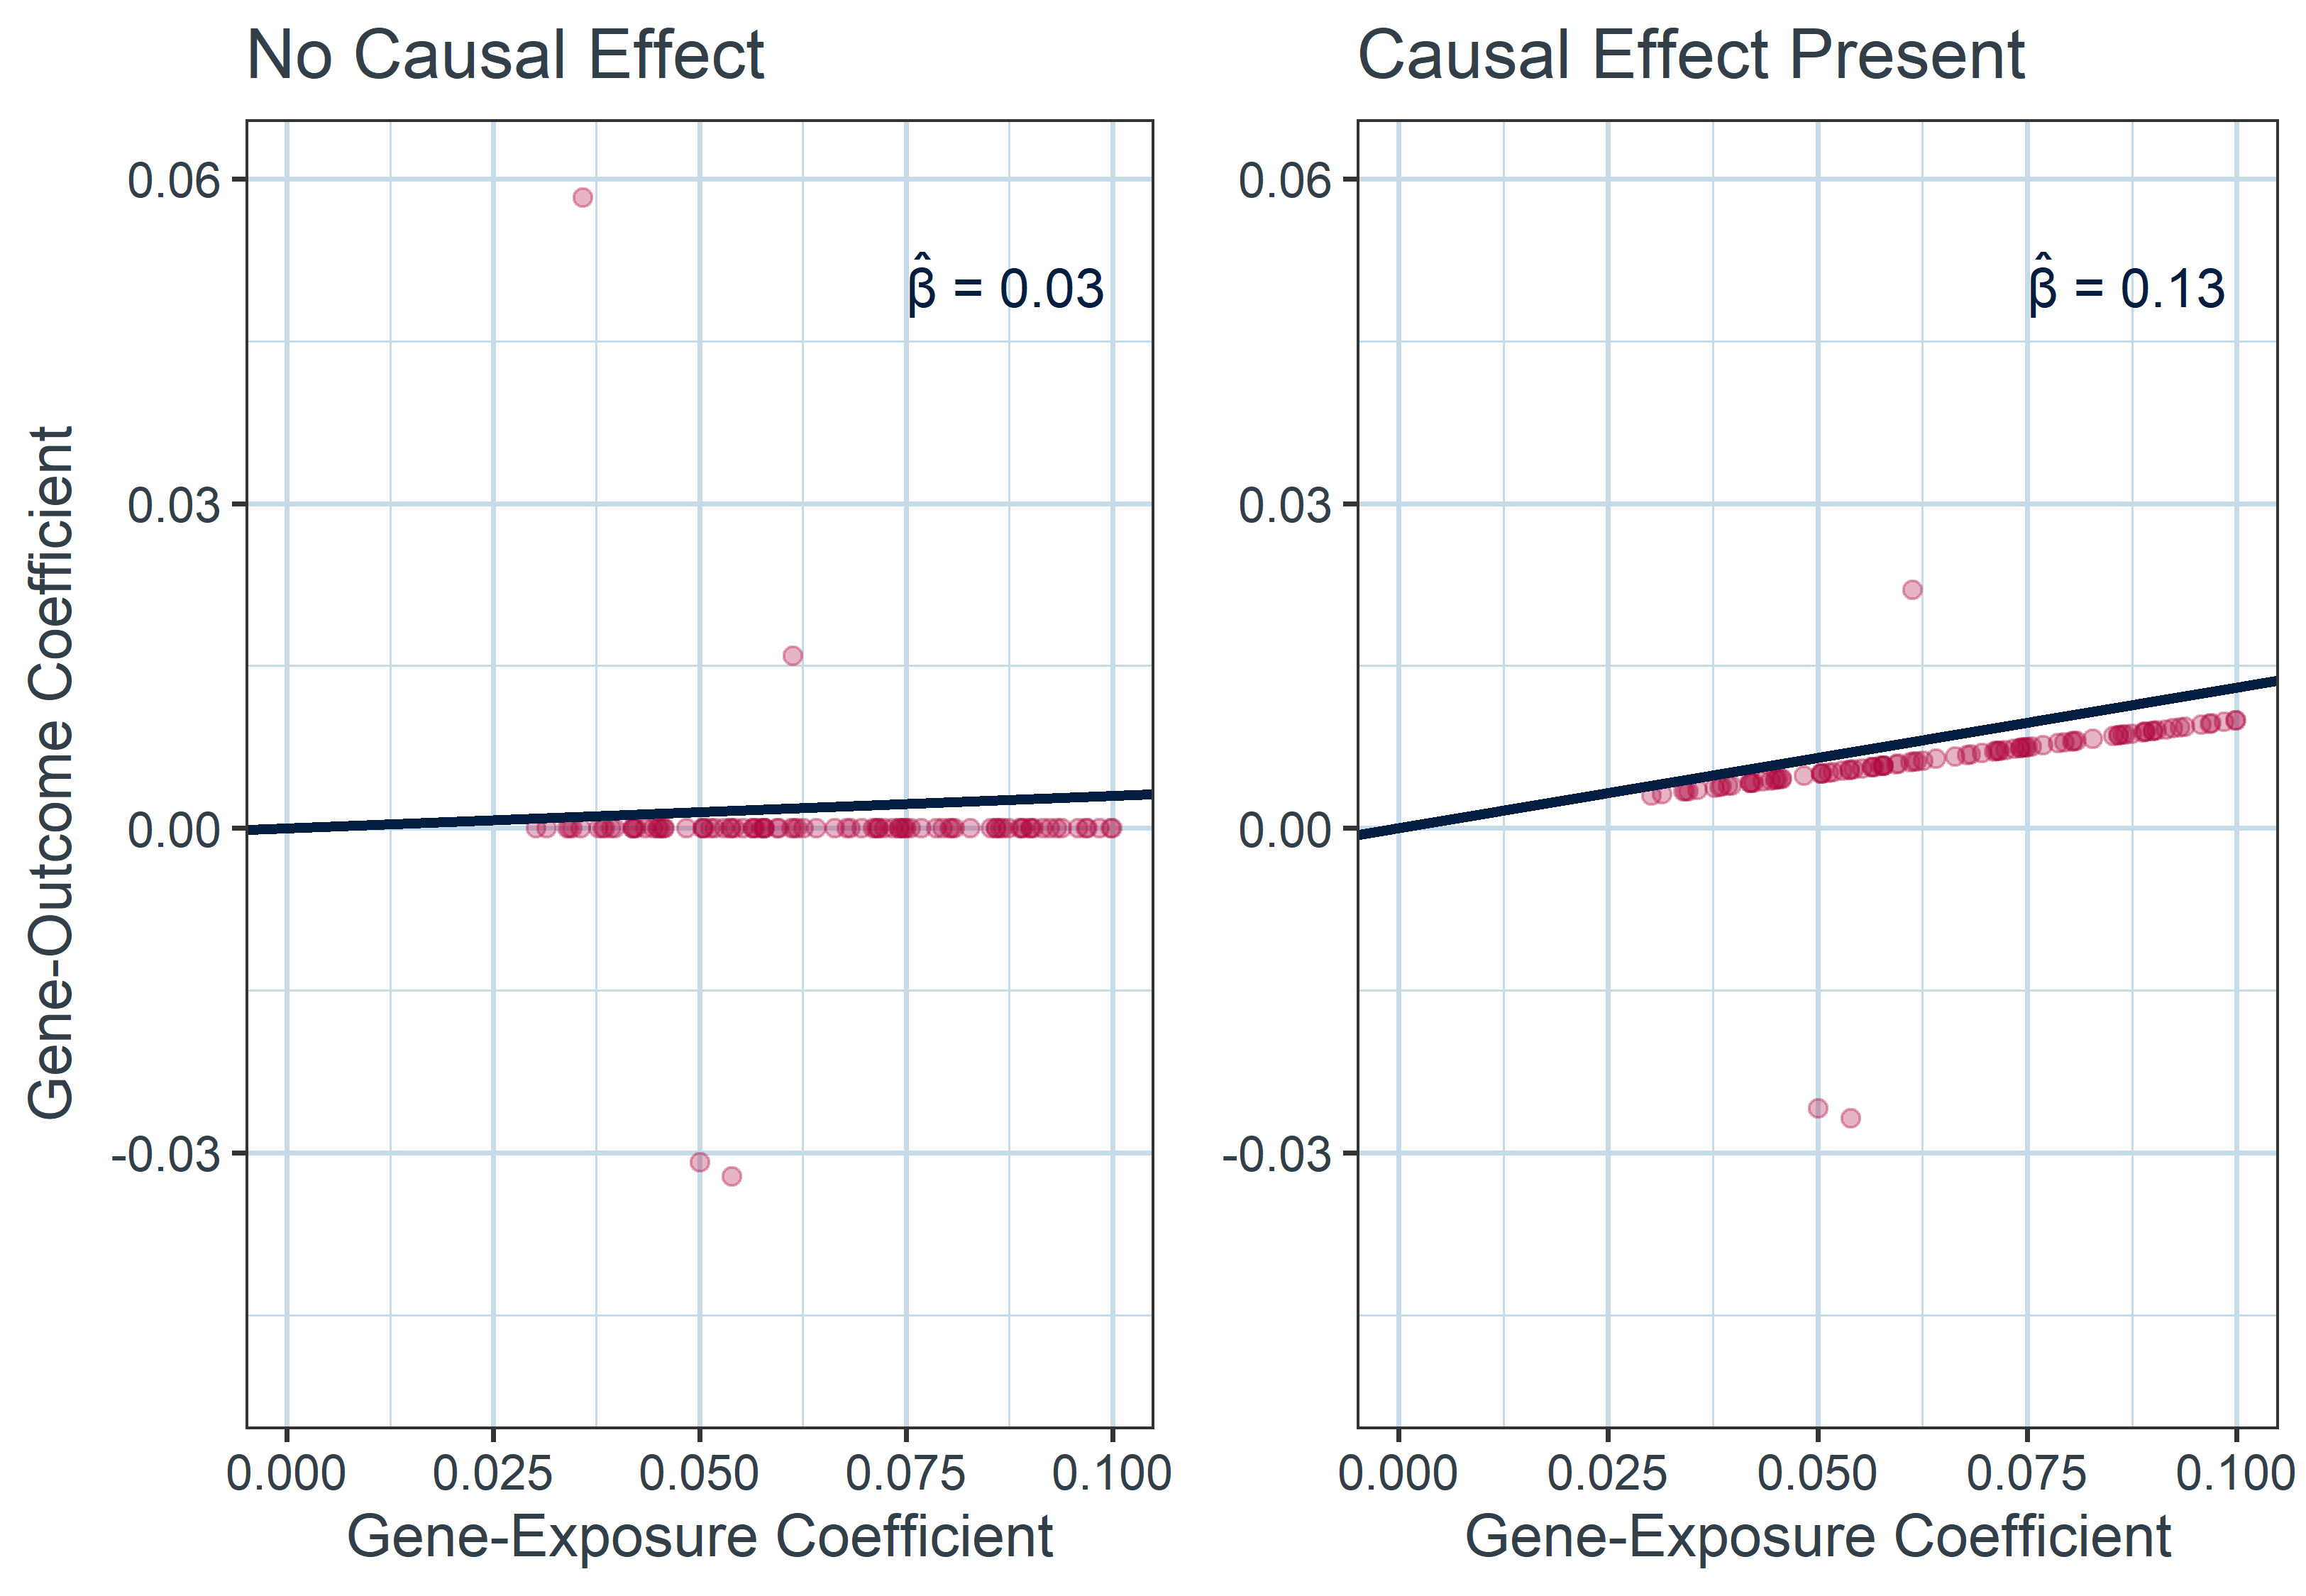
\includegraphics[keepaspectratio]{MSc_Thesis_Bookdown_files/figure-latex/test-plot-causal-inval-1.png}}

\newpage

\subsubsection{Balanced Versus Directional Pleiotropy}\label{balanced-versus-directional-pleiotropy}

\leavevmode\newline Replotting the above with unbalanced pleiotropy present (\texttt{balanced\_pleio\ =\ FALSE}), the invalid instruments should all appear as outliers in the positive direction, i.e.~steepening the line of best fit and leading to overestimation of the causal effect:

\pandocbounded{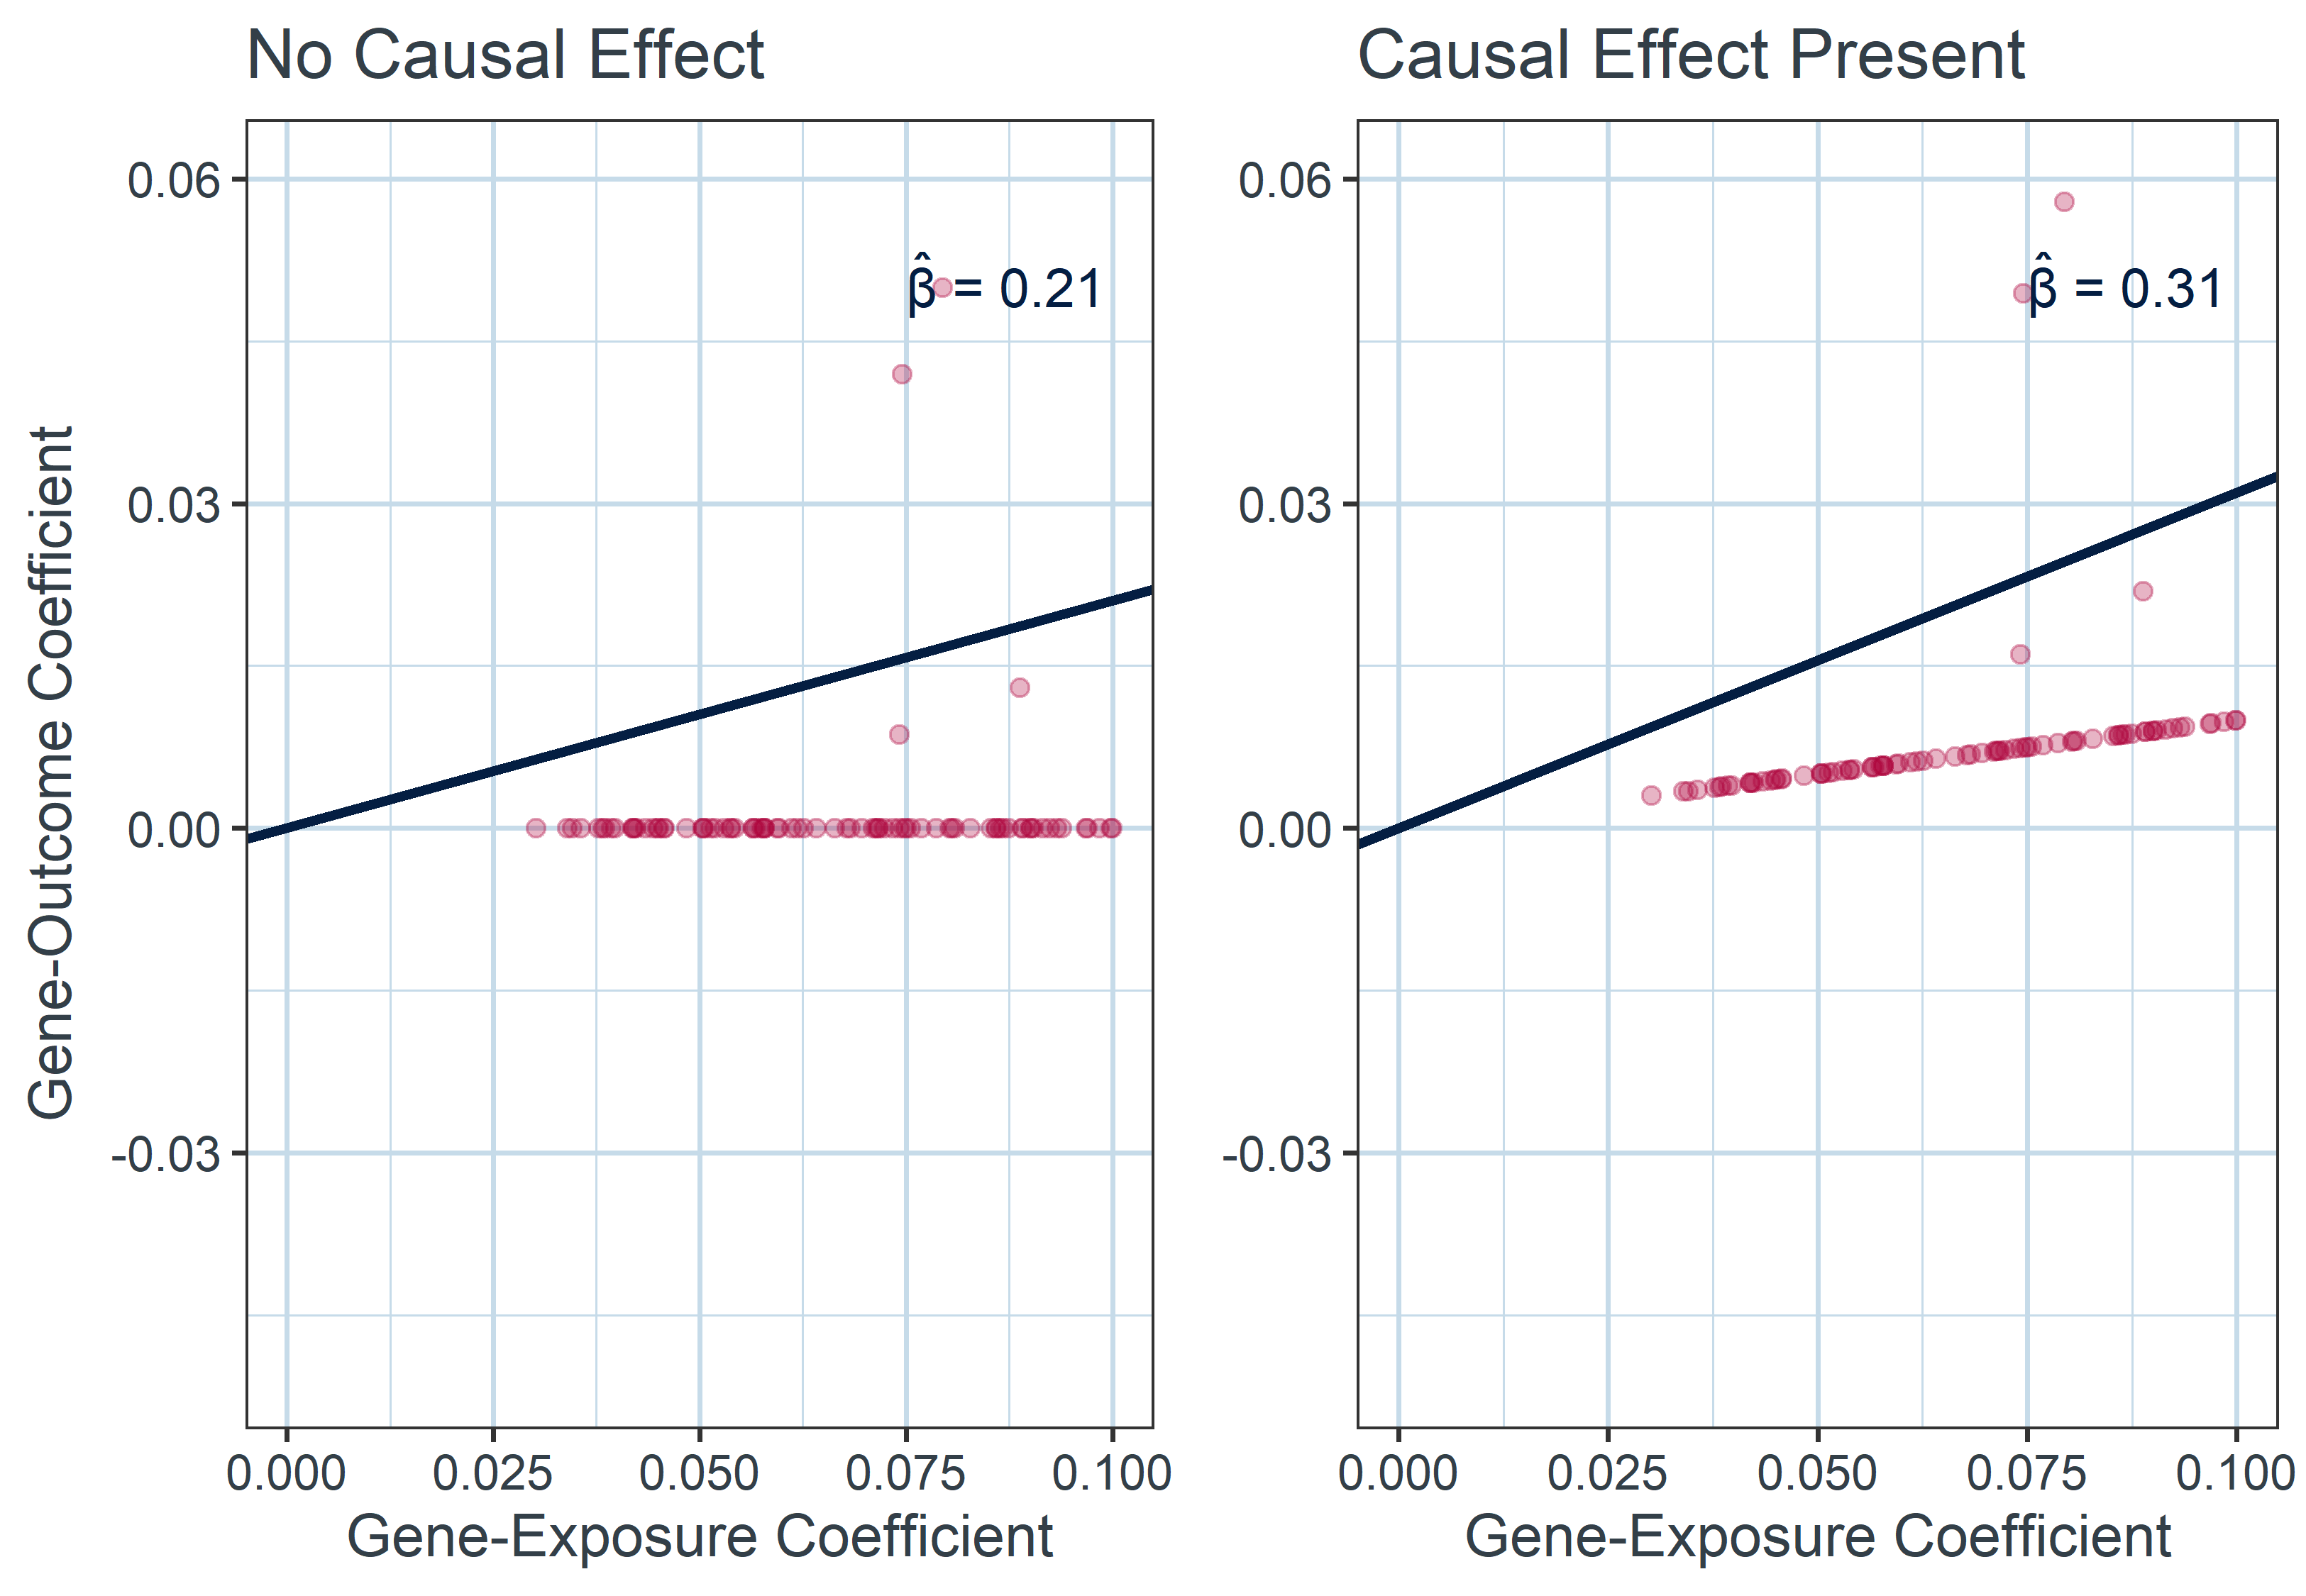
\includegraphics[keepaspectratio]{MSc_Thesis_Bookdown_files/figure-latex/test-plot-causal-unbal-1.png}}

\newpage

\subsubsection{InSIDE Assumption and Phi}\label{inside-assumption-and-phi}

\leavevmode\newline The variable phi represents additional pleiotropic effects of each invalid instrument when the \hyperref[acronyms_InSIDE]{InSIDE} assumption is not satisfied. The \hyperref[acronyms_InSIDE]{InSIDE} assumption states that the gene-exposure association is not correlated with the pleiotropic path gene-outcome path of any invalid genetic instruments. This assumption can be violated if e.g.:

\begin{itemize}
\item
  several invalid genetic instruments influence the outcome via the same pleiotropic path
\item
  several invalid genetic instruments are related to the same (unmeasured) confounders of the exposure:outcome relationship, aka correlated pleiotropy.
\end{itemize}

As such, when the \hyperref[acronyms_InSIDE]{InSIDE} assumption is violated, even ``strong'' instruments (i.e.~those with a strong gene-exposure relationship) may not allow accurate estimation of the true causal effect, as pleiotropic effects may scale with instrument strength. If pleiotropic effects are balanced, InSIDE assumption violation may lead to greater imprecision in causal effect estimation; if pleiotropic effects are directional, \hyperref[acronyms_InSIDE]{InSIDE} assumption violation may lead to bias.

Bowden et al\textsuperscript{\citeproc{ref-bowden_consistent_2016}{8}} modeled phi as the pleiotropic effects of unmeasured genetic confounders of the exposure:outcome relationship. Phi adds additional error to causal effect estimation in scenarios with directional pleiotropic effects (\texttt{0\ \textless{}\ alpha\ \textless{}\ 0.2}) and \hyperref[acronyms_InSIDE]{InSIDE} assumption violation. As such, switching \texttt{InSIDE\_satisfied} from \texttt{TRUE} to \texttt{FALSE} should add scatter to the linear association expected when plotting alpha versus gene-outcome coefficients with random error terms set to zero:

\pandocbounded{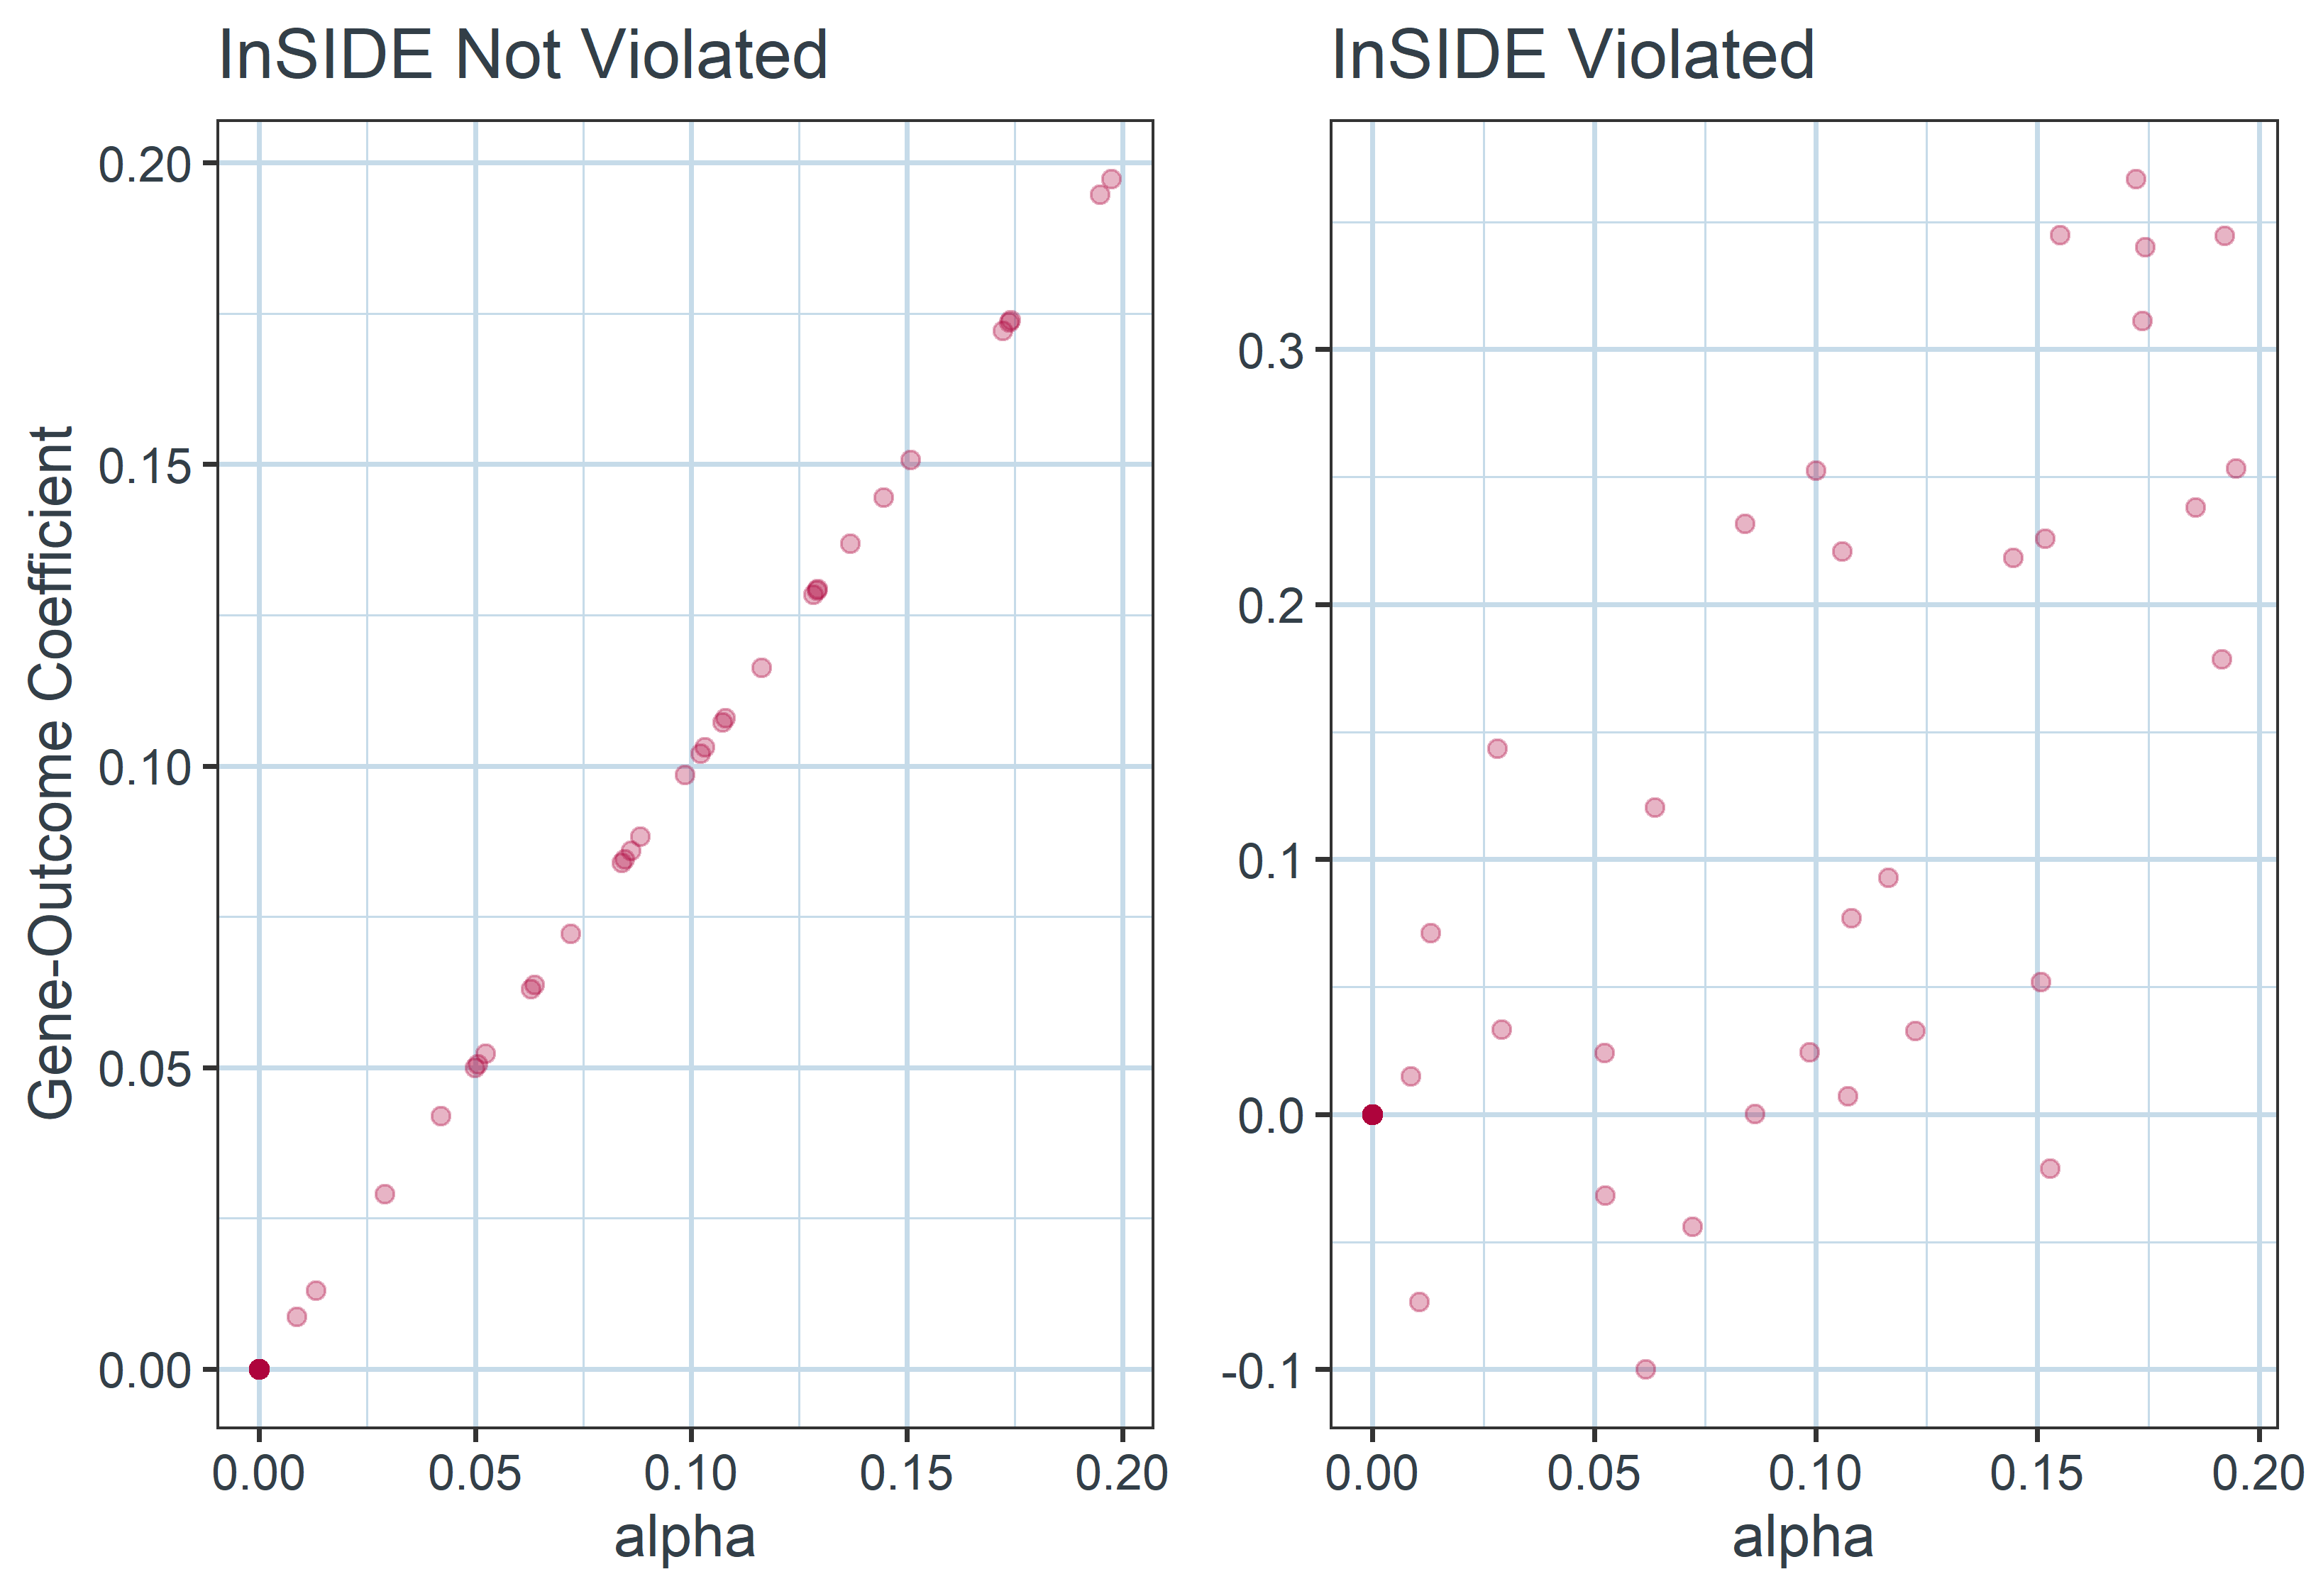
\includegraphics[keepaspectratio]{MSc_Thesis_Bookdown_files/figure-latex/test-plot-phi-1.png}}

\newpage

Setting \texttt{InSIDE\_satisfied\ =\ TRUE} should mean \texttt{phi\ =\ 0}; \texttt{InSIDE\_satisfied=FALSE} should result in \texttt{phi} \(\propto\) gene-outcome coefficient, with scatter only in the positive direction of gene-outcome coefficients given the model also requires directional pleiotropy before \texttt{phi} is used:

\pandocbounded{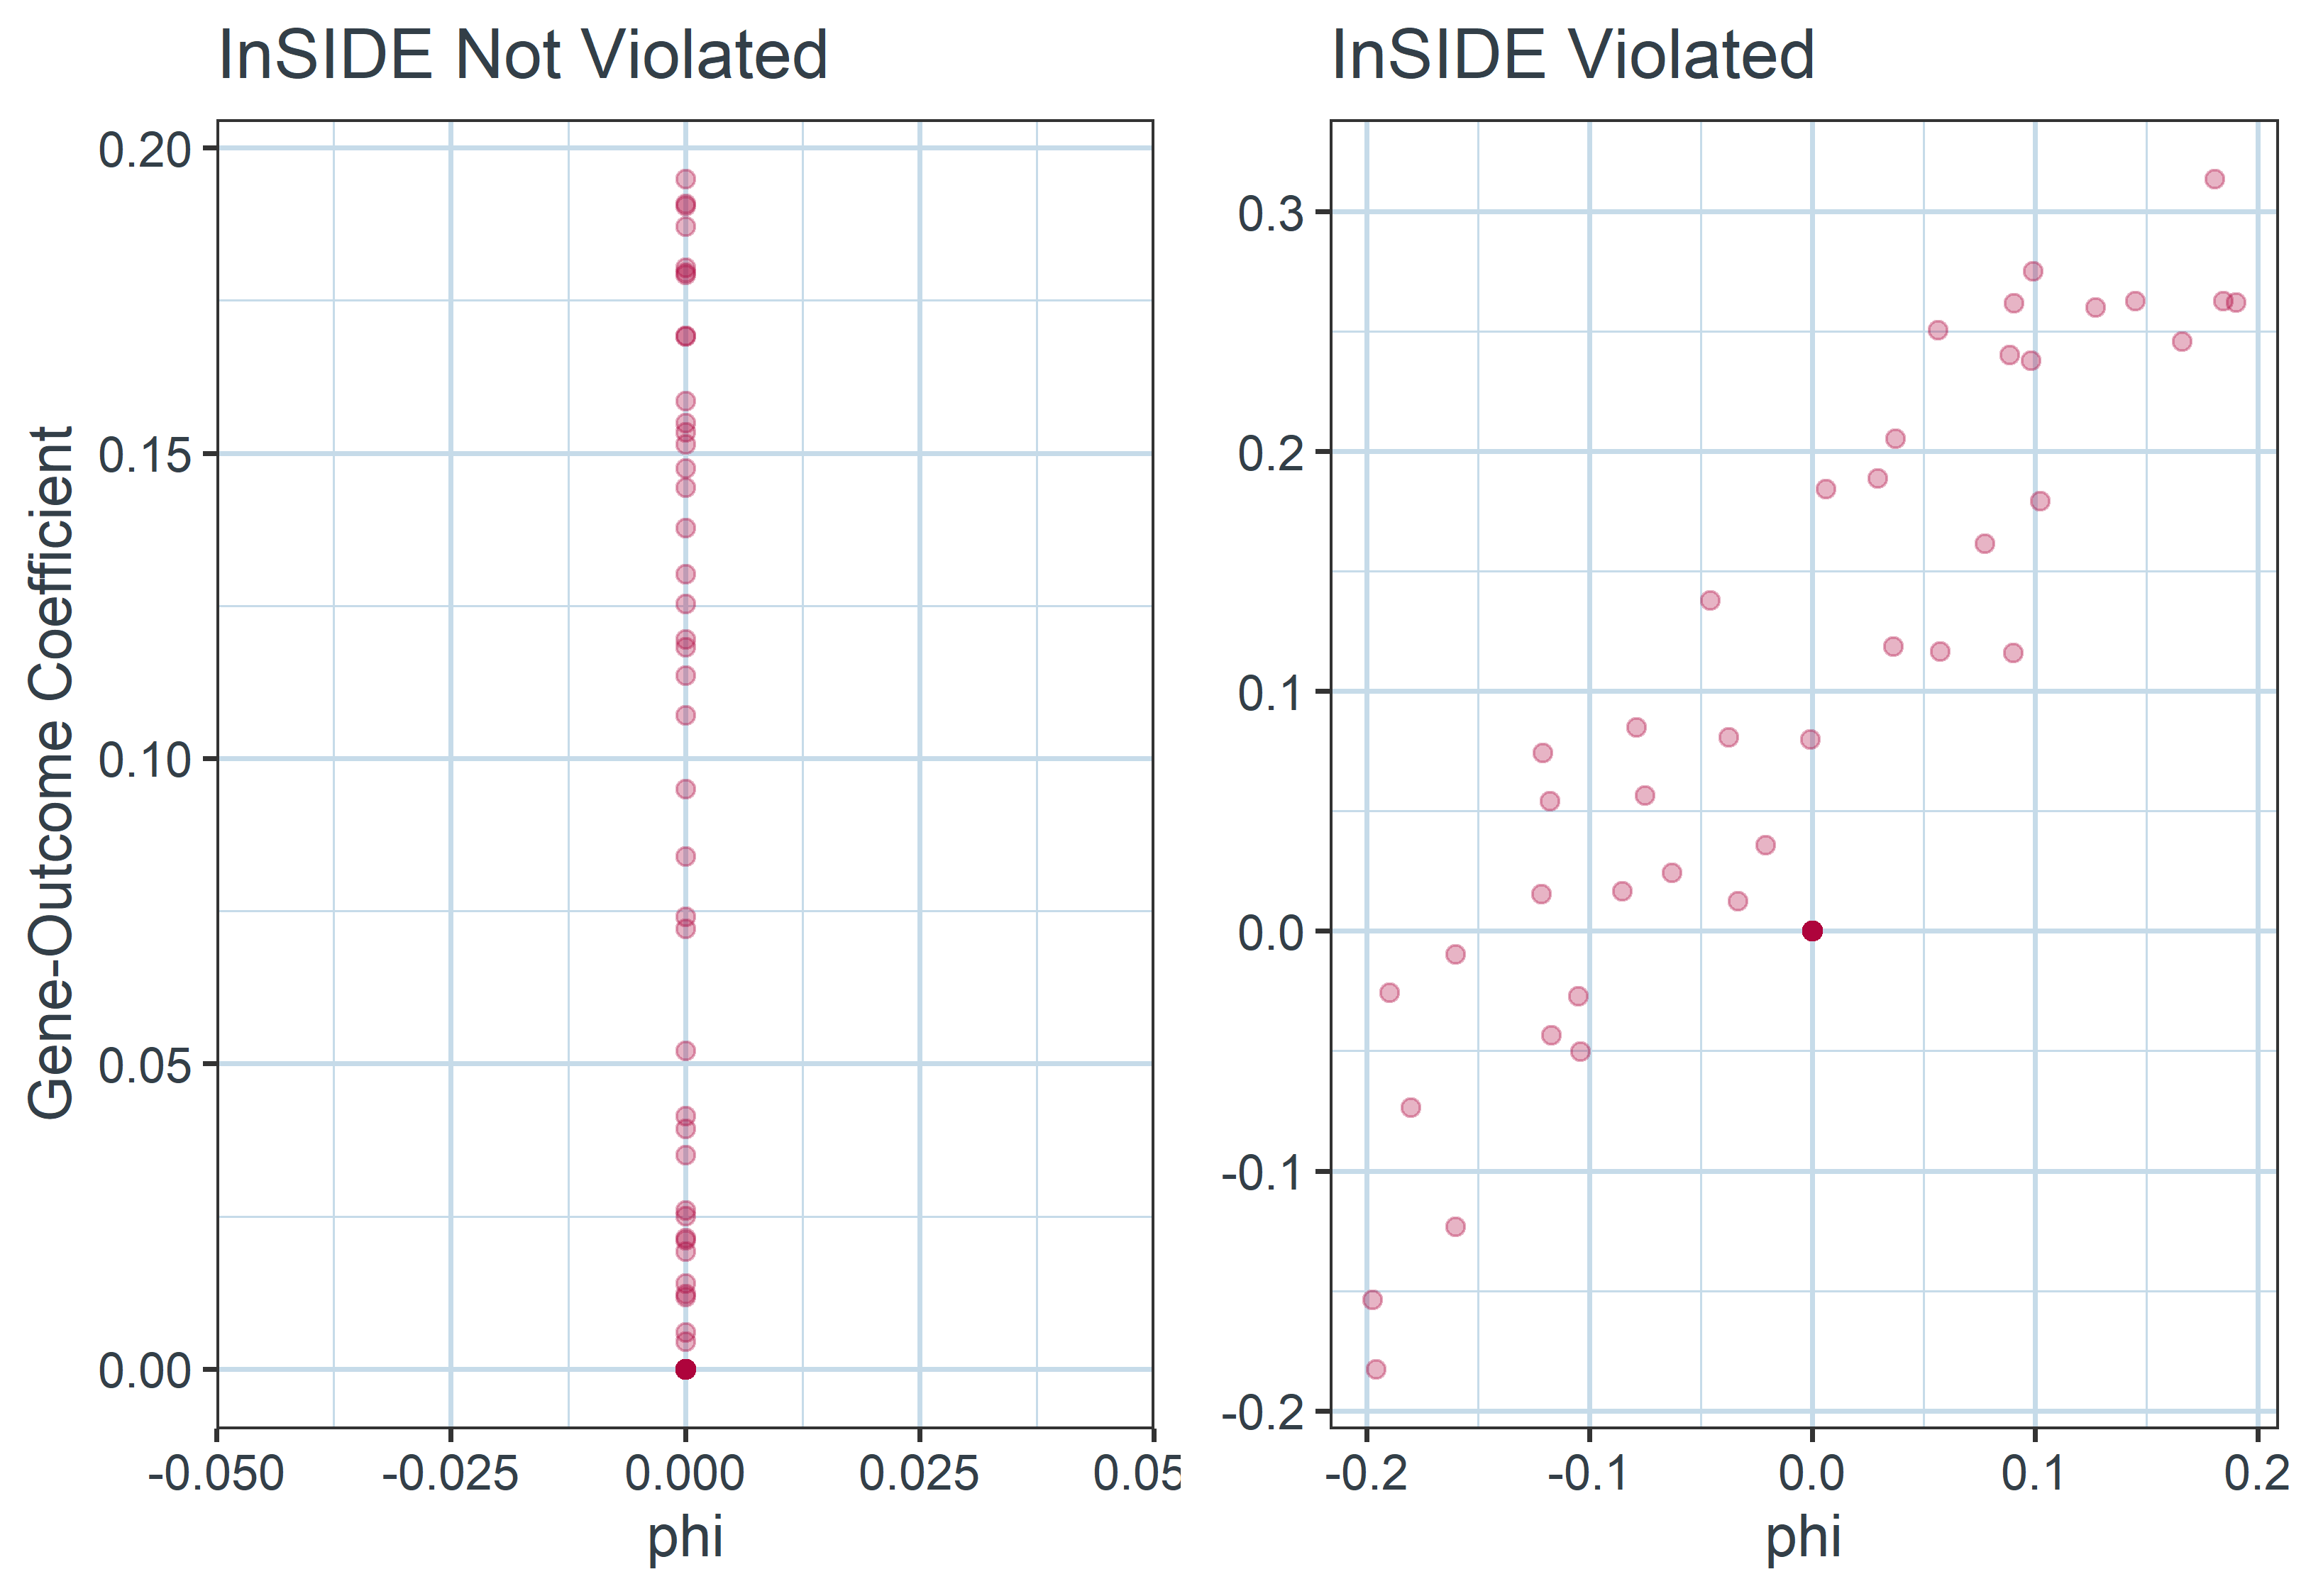
\includegraphics[keepaspectratio]{MSc_Thesis_Bookdown_files/figure-latex/test-plot-phi-2-1.png}}

\newpage

\subsection{Summary Table}\label{appendix-sim-summ}

A function (\texttt{get\_summary\_MR\_tib\_row}) was written to take models generated from each simulated dataset, estimate causal effect using both weighted median and MR-Hevo methodologies, then output a summary formatted as per Tables 2 \& 3 in Bowden et al\textsuperscript{\citeproc{ref-bowden_consistent_2016}{8}}:

\begin{Shaded}
\begin{Highlighting}[]
\CommentTok{\# Load WME functions}
\FunctionTok{library}\NormalTok{(TwoSampleMR)}

\CommentTok{\# Load RStan {-} needed for MR{-}Hevo}
\FunctionTok{library}\NormalTok{(rstan)}


\CommentTok{\# Run local copy of MR{-}Hevo functions}
\CommentTok{\# Not using full package due to conflicts with Windows}
\FunctionTok{source}\NormalTok{(here}\SpecialCharTok{::}\FunctionTok{here}\NormalTok{(}\StringTok{"Script"}\NormalTok{, }\StringTok{"Hevo"}\NormalTok{, }\StringTok{"functions.mrhevo.R"}\NormalTok{))}

\CommentTok{\# Standard set{-}up for RStan}
\FunctionTok{options}\NormalTok{(}\AttributeTok{mc.cores =}\NormalTok{ parallel}\SpecialCharTok{::}\FunctionTok{detectCores}\NormalTok{())}
\FunctionTok{rstan\_options}\NormalTok{(}\AttributeTok{auto\_write =} \ConstantTok{TRUE}\NormalTok{, }\AttributeTok{save\_dso =} \ConstantTok{TRUE}\NormalTok{)}


\CommentTok{\# Compile model for MR{-}Hevo}
\NormalTok{mr.stanmodel }\OtherTok{\textless{}{-}} \FunctionTok{stan\_model}\NormalTok{(}\AttributeTok{file=}\NormalTok{ here}\SpecialCharTok{::}\FunctionTok{here}\NormalTok{(}\StringTok{"Script"}\NormalTok{, }
                                      \StringTok{"Hevo"}\NormalTok{, }
                                      \StringTok{"MRHevo\_summarystats.stan"}\NormalTok{),}
                           \AttributeTok{model\_name=}\StringTok{"MRHevo.summarystats"}\NormalTok{, }
                           \AttributeTok{verbose=}\ConstantTok{FALSE}\NormalTok{,}
                           \AttributeTok{save\_dso =} \ConstantTok{TRUE}\NormalTok{,}
                           \AttributeTok{auto\_write =} \ConstantTok{TRUE}\NormalTok{)}

\NormalTok{get\_summary\_MR\_tib\_row }\OtherTok{\textless{}{-}} \ControlFlowTok{function}\NormalTok{(model\_list)\{}
  
  
  \CommentTok{\# Create output tibble in same format as Table 2/3 from}
  \CommentTok{\# Bowden et al}
\NormalTok{  output\_tib\_row }\OtherTok{\textless{}{-}} \FunctionTok{tibble}\NormalTok{(}\AttributeTok{N =} \FunctionTok{as.integer}\NormalTok{(),}
                           \AttributeTok{Prop\_Invalid =} \FunctionTok{as.double}\NormalTok{(),}
                           \AttributeTok{F\_stat =} \FunctionTok{as.double}\NormalTok{(),}
                           \AttributeTok{R2\_stat =} \FunctionTok{as.double}\NormalTok{(),}
                           \AttributeTok{WME\_Av =} \FunctionTok{as.double}\NormalTok{(),}
                           \AttributeTok{WME\_SE =} \FunctionTok{as.double}\NormalTok{(),}
                           \AttributeTok{WME\_Pos\_Rate =} \FunctionTok{as.double}\NormalTok{(),}
                           \AttributeTok{Hevo\_Av =} \FunctionTok{as.double}\NormalTok{(),}
                           \AttributeTok{Hevo\_SE =} \FunctionTok{as.double}\NormalTok{(),}
                           \AttributeTok{Hevo\_Pos\_Rate =} \FunctionTok{as.double}\NormalTok{())}
  
\NormalTok{  n\_datasets }\OtherTok{\textless{}{-}} \FunctionTok{length}\NormalTok{(model\_list)}
  
  \CommentTok{\# Create blank tibble to receive results of Weighted}
  \CommentTok{\# Median Estimator function from MR{-}Base}
  
\NormalTok{  results\_tib }\OtherTok{\textless{}{-}}  \FunctionTok{tibble}\NormalTok{(}\AttributeTok{WME\_est =} \FunctionTok{as.double}\NormalTok{(),}
                         \AttributeTok{WME\_se =} \FunctionTok{as.double}\NormalTok{(),}
                         \AttributeTok{WME\_pval =} \FunctionTok{as.double}\NormalTok{(),}
                         \AttributeTok{WME\_nsnp =} \FunctionTok{as.integer}\NormalTok{(),}
                         \AttributeTok{Hevo\_est =} \FunctionTok{as.double}\NormalTok{(),}
                         \AttributeTok{Hevo\_se =} \FunctionTok{as.double}\NormalTok{(),}
                         \AttributeTok{Hevo\_sd =} \FunctionTok{as.double}\NormalTok{(),}
                         \AttributeTok{Hevo\_est\_lower\_CI =} \FunctionTok{as.double}\NormalTok{(),}
                         \AttributeTok{Hevo\_est\_upper\_CI =} \FunctionTok{as.double}\NormalTok{(),}
                         \AttributeTok{Hevo\_causal\_detected =} \FunctionTok{as.logical}\NormalTok{()}
\NormalTok{  )}
  
  
  \CommentTok{\# Run WME and MR{-}Hevo for each dataset }
  \ControlFlowTok{for}\NormalTok{(dataset }\ControlFlowTok{in} \DecValTok{1}\SpecialCharTok{:}\NormalTok{n\_datasets)\{}
    
    \CommentTok{\# Stored as individual vectors for MR{-}Hevo/RStan {-} not}
    \CommentTok{\# Tidyverse compatible}
\NormalTok{    coeff\_G\_X\_vect }\OtherTok{\textless{}{-}}\NormalTok{ model\_list[[dataset]]}\SpecialCharTok{$}\NormalTok{coeff\_G\_X}
\NormalTok{    coeff\_G\_Y\_vect }\OtherTok{\textless{}{-}}\NormalTok{ model\_list[[dataset]]}\SpecialCharTok{$}\NormalTok{coeff\_G\_Y}
\NormalTok{    coeff\_G\_X\_SE\_vect }\OtherTok{\textless{}{-}}\NormalTok{ model\_list[[dataset]]}\SpecialCharTok{$}\NormalTok{coeff\_G\_X\_SE}
\NormalTok{    coeff\_G\_Y\_SE\_vect }\OtherTok{\textless{}{-}}\NormalTok{ model\_list[[dataset]]}\SpecialCharTok{$}\NormalTok{coeff\_G\_Y\_SE}
\NormalTok{    prop\_invalid }\OtherTok{\textless{}{-}} \FunctionTok{min}\NormalTok{(model\_list[[dataset]]}\SpecialCharTok{$}\NormalTok{prop\_invalid)}
\NormalTok{    F\_stat }\OtherTok{\textless{}{-}} \FunctionTok{min}\NormalTok{(model\_list[[dataset]]}\SpecialCharTok{$}\NormalTok{F\_stat)}
\NormalTok{    R2\_stat }\OtherTok{\textless{}{-}} \FunctionTok{min}\NormalTok{(model\_list[[dataset]]}\SpecialCharTok{$}\NormalTok{R2\_stat)}
\NormalTok{    n\_instruments }\OtherTok{\textless{}{-}} \FunctionTok{max}\NormalTok{(model\_list[[dataset]]}\SpecialCharTok{$}\NormalTok{Instrument)}
\NormalTok{    n\_participants }\OtherTok{\textless{}{-}} \FunctionTok{min}\NormalTok{(model\_list[[dataset]]}\SpecialCharTok{$}\NormalTok{n\_participants)}
    
    
    \CommentTok{\# N.B. MR{-}Hevo terminology vs WME paper/other code:}
    \CommentTok{\# alpha = effects of instruments on exposure, i.e. coeff\_G\_X}
    \CommentTok{\# beta = pleiotropic effects of instruments on outcome, i.e. alpha in WME}
    \CommentTok{\# gamma = effects of instruments on outcome, i.e. coeff\_G\_Y}
    \CommentTok{\# theta = causal effect X on Y, i.e. b}
    
    \CommentTok{\# Results from weighted median estimator method}
\NormalTok{    WME\_results }\OtherTok{\textless{}{-}} \FunctionTok{mr\_weighted\_median}\NormalTok{(}\AttributeTok{b\_exp =}\NormalTok{ coeff\_G\_X\_vect,}
                                      \AttributeTok{b\_out =}\NormalTok{ coeff\_G\_Y\_vect,}
                                      \AttributeTok{se\_exp =}\NormalTok{ coeff\_G\_X\_SE\_vect,}
                                      \AttributeTok{se\_out =}\NormalTok{ coeff\_G\_Y\_SE\_vect,}
                                      \AttributeTok{parameters =} \FunctionTok{list}\NormalTok{(}\AttributeTok{nboot =} \DecValTok{1000}\NormalTok{))}
    
    \CommentTok{\# Results from MR{-}Hevo method}
\NormalTok{    Hevo\_results}\OtherTok{\textless{}{-}} \FunctionTok{run\_mrhevo.sstats}\NormalTok{(}\AttributeTok{alpha\_hat =}\NormalTok{ coeff\_G\_X\_vect,}
                                    \AttributeTok{se.alpha\_hat =}\NormalTok{ coeff\_G\_X\_SE\_vect,}
                                    \AttributeTok{gamma\_hat =}\NormalTok{ coeff\_G\_Y\_vect,}
                                    \AttributeTok{se.gamma\_hat =}\NormalTok{ coeff\_G\_Y\_SE\_vect) }\SpecialCharTok{\%\textgreater{}\%}
     \FunctionTok{summary}\NormalTok{()}
    
    
    \CommentTok{\# Extract WME Results}
\NormalTok{    results\_tib[dataset, ]}\SpecialCharTok{$}\NormalTok{WME\_est }\OtherTok{\textless{}{-}}\NormalTok{ WME\_results}\SpecialCharTok{$}\NormalTok{b}
\NormalTok{    results\_tib[dataset, ]}\SpecialCharTok{$}\NormalTok{WME\_se }\OtherTok{\textless{}{-}}\NormalTok{ WME\_results}\SpecialCharTok{$}\NormalTok{se}
\NormalTok{    results\_tib[dataset, ]}\SpecialCharTok{$}\NormalTok{WME\_pval }\OtherTok{\textless{}{-}}\NormalTok{ WME\_results}\SpecialCharTok{$}\NormalTok{pval}
\NormalTok{    results\_tib[dataset, ]}\SpecialCharTok{$}\NormalTok{WME\_nsnp }\OtherTok{\textless{}{-}}\NormalTok{ WME\_results}\SpecialCharTok{$}\NormalTok{nsnp}
    
    \CommentTok{\# Extract MR{-}Hevo Results}
\NormalTok{    results\_tib[dataset, ]}\SpecialCharTok{$}\NormalTok{Hevo\_est }\OtherTok{\textless{}{-}}\NormalTok{ Hevo\_results}\SpecialCharTok{$}\NormalTok{summary[}\StringTok{"theta"}\NormalTok{,}\StringTok{"mean"}\NormalTok{]}
\NormalTok{    results\_tib[dataset, ]}\SpecialCharTok{$}\NormalTok{Hevo\_se }\OtherTok{\textless{}{-}}\NormalTok{ Hevo\_results}\SpecialCharTok{$}\NormalTok{summary[}\StringTok{"theta"}\NormalTok{,}\StringTok{"se\_mean"}\NormalTok{]}
\NormalTok{    results\_tib[dataset, ]}\SpecialCharTok{$}\NormalTok{Hevo\_sd }\OtherTok{\textless{}{-}}\NormalTok{ Hevo\_results}\SpecialCharTok{$}\NormalTok{summary[}\StringTok{"theta"}\NormalTok{,}\StringTok{"sd"}\NormalTok{]}
\NormalTok{    results\_tib[dataset, ]}\SpecialCharTok{$}\NormalTok{Hevo\_est\_lower\_CI }\OtherTok{\textless{}{-}}\NormalTok{ Hevo\_results}\SpecialCharTok{$}\NormalTok{summary[}\StringTok{"theta"}\NormalTok{,}\StringTok{"2.5\%"}\NormalTok{]}
\NormalTok{    results\_tib[dataset, ]}\SpecialCharTok{$}\NormalTok{Hevo\_est\_upper\_CI }\OtherTok{\textless{}{-}}\NormalTok{ Hevo\_results}\SpecialCharTok{$}\NormalTok{summary[}\StringTok{"theta"}\NormalTok{,}\StringTok{"97.5\%"}\NormalTok{]}
    
\NormalTok{  \}}
  
  \CommentTok{\# Add causality Boolean to MR{-}Hevo}
\NormalTok{  results\_tib }\OtherTok{\textless{}{-}}\NormalTok{ results\_tib }\SpecialCharTok{\%\textgreater{}\%}
   \FunctionTok{mutate}\NormalTok{(}\AttributeTok{Hevo\_est\_causal\_detected =}\NormalTok{ (Hevo\_est\_lower\_CI }\SpecialCharTok{\textgreater{}} \DecValTok{0}  \SpecialCharTok{|}\NormalTok{ Hevo\_est\_upper\_CI }\SpecialCharTok{\textless{}} \DecValTok{0}\NormalTok{))}
  
  
\NormalTok{  output\_tib\_row }\OtherTok{\textless{}{-}}\NormalTok{ results\_tib }\SpecialCharTok{\%\textgreater{}\%} 
    \FunctionTok{summarise}\NormalTok{(}\AttributeTok{N =}\NormalTok{ n\_participants,}
              \AttributeTok{Prop\_Invalid =}\NormalTok{ prop\_invalid,}
              \AttributeTok{F\_stat =} \FunctionTok{mean}\NormalTok{(F\_stat),}
              \AttributeTok{R2\_stat =} \FunctionTok{mean}\NormalTok{(R2\_stat),}
              \AttributeTok{WME\_Av =} \FunctionTok{mean}\NormalTok{(WME\_est),}
              \AttributeTok{WME\_SE =} \FunctionTok{mean}\NormalTok{(WME\_se),}
              \AttributeTok{WME\_Pos\_Rate =} \FunctionTok{length}\NormalTok{(WME\_pval[WME\_pval }\SpecialCharTok{\textless{}} \FloatTok{0.05}\NormalTok{]) }\SpecialCharTok{/}\NormalTok{ n\_datasets,}
              \AttributeTok{Hevo\_Av =} \FunctionTok{mean}\NormalTok{(Hevo\_est),}
              \AttributeTok{Hevo\_SE =} \FunctionTok{mean}\NormalTok{(Hevo\_se),}
              \AttributeTok{Hevo\_Lower\_CI =} \FunctionTok{mean}\NormalTok{(Hevo\_est\_lower\_CI),}
              \AttributeTok{Hevo\_Upper\_CI =} \FunctionTok{mean}\NormalTok{(Hevo\_est\_upper\_CI),}
              \AttributeTok{Hevo\_Pos\_Rate =} \FunctionTok{sum}\NormalTok{(Hevo\_est\_causal\_detected) }\SpecialCharTok{/}\NormalTok{ n\_datasets}
\NormalTok{    ) }\SpecialCharTok{\%\textgreater{}\%} 
    \FunctionTok{mutate}\NormalTok{(}\FunctionTok{across}\NormalTok{(where}\SpecialCharTok{::}\FunctionTok{here}\NormalTok{(is.double), round, }\DecValTok{3}\NormalTok{))}
  
  \FunctionTok{return}\NormalTok{(output\_tib\_row)}
  
\NormalTok{\}}
\end{Highlighting}
\end{Shaded}

\begin{Shaded}
\begin{Highlighting}[]
\NormalTok{test\_tib\_summ\_MR\_data }\OtherTok{\textless{}{-}}  \FunctionTok{get\_simulated\_MR\_data}\NormalTok{(}\AttributeTok{n\_participants =} \DecValTok{10000}\NormalTok{,}
                                                \AttributeTok{n\_instruments =} \DecValTok{25}\NormalTok{,}
                                                \AttributeTok{n\_datasets =} \DecValTok{2}\NormalTok{,}
                                                \AttributeTok{prop\_invalid =} \FloatTok{0.1}\NormalTok{,}
                                                \AttributeTok{beta\_val =} \FloatTok{0.1}\NormalTok{,}
                                                \AttributeTok{causal\_effect =} \ConstantTok{TRUE}\NormalTok{,}
                                                \AttributeTok{rand\_error =} \ConstantTok{TRUE}\NormalTok{,}
                                                \AttributeTok{two\_sample =} \ConstantTok{TRUE}\NormalTok{,}
                                                \AttributeTok{balanced\_pleio =} \ConstantTok{TRUE}\NormalTok{,}
                                                \AttributeTok{InSIDE\_satisfied =} \ConstantTok{TRUE}\NormalTok{)}

\NormalTok{test\_tib\_summ\_MR\_models }\OtherTok{\textless{}{-}} \FunctionTok{get\_models}\NormalTok{(test\_tib\_summ\_MR\_data)}

\NormalTok{test\_tib\_summ\_MR\_row }\OtherTok{\textless{}{-}} \FunctionTok{get\_summary\_MR\_tib\_row}\NormalTok{(test\_tib\_summ\_MR\_models)}
\end{Highlighting}
\end{Shaded}

\begin{verbatim}
## 
## CHECKING DATA AND PREPROCESSING FOR MODEL 'MRHevo.summarystats' NOW.
## 
## COMPILING MODEL 'MRHevo.summarystats' NOW.
## 
## STARTING SAMPLER FOR MODEL 'MRHevo.summarystats' NOW.
\end{verbatim}

\begin{verbatim}
## 
## CHECKING DATA AND PREPROCESSING FOR MODEL 'MRHevo.summarystats' NOW.
## 
## COMPILING MODEL 'MRHevo.summarystats' NOW.
## 
## STARTING SAMPLER FOR MODEL 'MRHevo.summarystats' NOW.
\end{verbatim}

\begin{Shaded}
\begin{Highlighting}[]
\NormalTok{test\_tib\_summ\_MR\_row }\SpecialCharTok{\%\textgreater{}\%} 
  \FunctionTok{kable}\NormalTok{() }\SpecialCharTok{\%\textgreater{}\%} 
  \FunctionTok{kable\_styling}\NormalTok{(}\AttributeTok{latex\_options=}\StringTok{"scale\_down"}\NormalTok{)}
\end{Highlighting}
\end{Shaded}

\begin{table}
\centering
\resizebox{\ifdim\width>\linewidth\linewidth\else\width\fi}{!}{
\begin{tabular}{r|r|r|r|r|r|r|r|r|r|r|r}
\hline
N & Prop\_Invalid & F\_stat & R2\_stat & WME\_Av & WME\_SE & WME\_Pos\_Rate & Hevo\_Av & Hevo\_SE & Hevo\_Lower\_CI & Hevo\_Upper\_CI & Hevo\_Pos\_Rate\\
\hline
10000 & 0.1 & 14.739 & 0.036 & 0.091 & 0.09 & 0.5 & 0.121 & 0.001 & -0.052 & 0.302 & 0\\
\hline
\end{tabular}}
\end{table}

\newpage

\section{Appendix: R Packages Used}\label{appendix-pkg}

\subsection{Package Citations}\label{package-citations}

This work was completed using R version 4.4.1\textsuperscript{\citeproc{ref-base}{21}} with the following R packages: acronymsdown v. 0.11.1\textsuperscript{\citeproc{ref-acronymsdown}{45}}, benchmarkme v. 1.0.8\textsuperscript{\citeproc{ref-benchmarkme}{46}}, biostats101 v. 0.1.1\textsuperscript{\citeproc{ref-biostats101}{47}}, bookdown v. 0.41\textsuperscript{\citeproc{ref-bookdown2016}{48},\citeproc{ref-bookdown2024}{49}}, car v. 3.1.3\textsuperscript{\citeproc{ref-car}{50}}, cowplot v. 1.1.3\textsuperscript{\citeproc{ref-cowplot}{51}}, crayon v. 1.5.3\textsuperscript{\citeproc{ref-crayon}{52}}, devtools v. 2.4.5\textsuperscript{\citeproc{ref-devtools}{53}}, flextable v. 0.9.9\textsuperscript{\citeproc{ref-flextable}{54}}, ftExtra v. 0.6.4\textsuperscript{\citeproc{ref-ftExtra}{55}}, ggdag v. 0.2.13\textsuperscript{\citeproc{ref-ggdag}{56}}, gghighlight v. 0.4.1\textsuperscript{\citeproc{ref-gghighlight}{57}}, gluedown v. 1.0.9\textsuperscript{\citeproc{ref-gluedown}{58}}, grateful v. 0.2.12\textsuperscript{\citeproc{ref-grateful}{59}}, grid v. 4.4.1\textsuperscript{\citeproc{ref-grid}{60}}, here v. 1.0.1\textsuperscript{\citeproc{ref-here}{61}}, infer v. 1.0.8\textsuperscript{\citeproc{ref-infer}{62}}, kableExtra v. 1.4.0\textsuperscript{\citeproc{ref-kableExtra}{63}}, knitr v. 1.50\textsuperscript{\citeproc{ref-knitr2014}{64}--\citeproc{ref-knitr2025}{66}}, matrixStats v. 1.4.1\textsuperscript{\citeproc{ref-matrixStats}{67}}, medicaldata v. 0.2.0\textsuperscript{\citeproc{ref-medicaldata}{44}}, officer v. 0.6.10\textsuperscript{\citeproc{ref-officer}{68}}, parallel v. 4.4.1\textsuperscript{\citeproc{ref-parallel}{69}}, rmarkdown v. 2.29\textsuperscript{\citeproc{ref-rmarkdown2018}{70}--\citeproc{ref-rmarkdown2024}{72}}, rstan v. 2.32.6\textsuperscript{\citeproc{ref-rstan}{73}}, tables v. 0.9.31\textsuperscript{\citeproc{ref-tables}{74}}, tidyverse v. 2.0.0\textsuperscript{\citeproc{ref-tidyverse}{23}}, TwoSampleMR v. 0.6.8\textsuperscript{\citeproc{ref-TwoSampleMR2017}{75},\citeproc{ref-TwoSampleMR2018}{76}}, where v. 1.0.0\textsuperscript{\citeproc{ref-where}{77}}, wordcountaddin v. 0.3.0.9000\textsuperscript{\citeproc{ref-wordcountaddin}{78}}.

\subsection{Session Information}\label{Session-Information}

CPU: 13th Gen Intel(R) Core(TM) i7-13700H, 20 cores \newline
RAM: 16.9 GB

\begin{verbatim}
##  setting  value
##  version  R version 4.4.3 (2025-02-28 ucrt)
##  os       Windows 11 x64 (build 26100)
##  system   x86_64, mingw32
##  ui       RStudio
##  language (EN)
##  collate  English_United Kingdom.utf8
##  ctype    English_United Kingdom.utf8
##  tz       Europe/London
##  date     2025-06-08
##  rstudio  2025.05.0+496 Mariposa Orchid (desktop)
##  pandoc   3.4 @ C:/Program Files/RStudio/resources/app/bin/quarto/bin/tools/ (via rmarkdown)
##  quarto   ERROR: Unknown command "TMPDIR=C:/Users/timol/AppData/Local/Temp/RtmpoL0HFL/file4d9c24bb4b5d". Did you mean command "remove"? @ C:\\PROGRA~1\\RStudio\\resources\\app\\bin\\quarto\\bin\\quarto.exe
\end{verbatim}

\begin{verbatim}
## # A tibble: 33 x 5
##    package     ondiskversion loadedversion date  source
##    <chr>       <chr>         <chr>         <chr> <chr> 
##  1 acronymsdo~ 0.11.1        0.11.1        2025~ Githu~
##  2 bookdown    0.43          0.43          2025~ CRAN ~
##  3 cowplot     1.1.3         1.1.3         2024~ CRAN ~
##  4 dplyr       1.1.4         1.1.4         2023~ CRAN ~
##  5 flextable   0.9.9         0.9.9         2025~ CRAN ~
##  6 forcats     1.0.0         1.0.0         2023~ CRAN ~
##  7 ftExtra     0.6.4         0.6.4         2024~ CRAN ~
##  8 ggdag       0.2.13        0.2.13        2024~ CRAN ~
##  9 gghighlight 0.4.1         0.4.1         2023~ CRAN ~
## 10 ggplot2     3.5.2         3.5.2         2025~ CRAN ~
## 11 gluedown    1.0.9         1.0.9         2024~ CRAN ~
## 12 grateful    0.2.12        0.2.12        2025~ CRAN ~
## 13 here        1.0.1         1.0.1         2020~ CRAN ~
## 14 infer       1.0.8         1.0.8         2025~ CRAN ~
## 15 kableExtra  1.4.0         1.4.0         2024~ CRAN ~
## 16 knitr       1.50          1.50          2025~ CRAN ~
## 17 koRpus      0.13.8        0.13-8        2021~ CRAN ~
## 18 koRpus.lan~ 0.1.4         0.1-4         2020~ CRAN ~
## 19 lubridate   1.9.4         1.9.4         2024~ CRAN ~
## 20 magrittr    2.0.3         2.0.3         2022~ CRAN ~
## 21 medicaldata 0.2.0         0.2.0         2021~ CRAN ~
## 22 officer     0.6.10        0.6.10        2025~ CRAN ~
## 23 purrr       1.0.4         1.0.4         2025~ CRAN ~
## 24 readr       2.1.5         2.1.5         2024~ CRAN ~
## 25 rstan       2.32.7        2.32.7        2025~ CRAN ~
## 26 StanHeaders 2.32.10       2.32.10       2024~ CRAN ~
## 27 stringr     1.5.1         1.5.1         2023~ CRAN ~
## 28 sylly       0.1.6         0.1-6         2020~ CRAN ~
## 29 tables      0.9.31        0.9.31        2024~ CRAN ~
## 30 tibble      3.2.1         3.2.1         2023~ CRAN ~
## 31 tidyr       1.3.1         1.3.1         2024~ CRAN ~
## 32 tidyverse   2.0.0         2.0.0         2023~ CRAN ~
## 33 TwoSampleMR 0.6.16        0.6.16        2025~ https~
\end{verbatim}

\newpage

\end{document}
